% ------------------------------------------------------------------------------
% ATLAS document header
% ------------------------------------------------------------------------------

\documentclass[11pt,twoside]{book}
\usepackage[paperwidth=17cm,paperheight=24cm,inner=25mm,outer=14mm,top=22mm,bottom=18mm]{geometry} % Marcos
\usepackage{fancyhdr}
\fancyhf{}
\fancyhead[LE]{\thepage}
\fancyhead[RE]{\textsl{E. Valiente Moreno}}
\fancyhead[RO]{\thepage}
\fancyhead[LO]{\nouppercase\leftmark}
\renewcommand{\headrulewidth}{0pt}
\renewcommand{\chaptermark}[1]{\markboth{\textsl{\thechapter.\ #1}}{}}

% List of acronyms
\usepackage[acronym]{glossaries}

% ------------------------------------------------------------------------------
% Packages
% ------------------------------------------------------------------------------

% Figure paths
\usepackage{amssymb}
\usepackage{placeins} % en el preámbulo
\usepackage[percent]{overpic} % en el preámbulo
\usepackage{pdflscape}  % en el preámbulo
\usepackage{rotating}
\usepackage[utf8]{inputenc}
\usepackage{graphicx}
\graphicspath{{images/}}
\usepackage[spanish,english]{babel}
\usepackage{subcaption}
\usepackage{adjustbox}
\usepackage{cite}
\usepackage{appendix}
\usepackage{lipsum}
\usepackage{booktabs}
\usepackage{xcolor}
\usepackage[makeroom]{cancel}
\usepackage{dsfont}
\usepackage{slashed}
\usepackage{xspace}
\usepackage[most]{tcolorbox}
\usepackage{tikz-feynman}
\usepackage{textcomp} % For writing symbols in normal text mode (not math mode)
\usepackage{multirow}
\usepackage{array}
\newcolumntype{P}[1]{>{\centering\arraybackslash}p{#1}}
\usepackage{bm}
\usepackage[pagebackref=true]{hyperref} % Golden rule: import this package the last one in the preamble
\hypersetup{
  colorlinks=true,
  citecolor=blue,  % color of links to bibliography
  urlcolor=blue,    % color of external links
}
\usepackage[font=small]{caption}

\renewcommand*{\backref}[1]{}
\renewcommand*{\backrefalt}[4]{(cit. on p. #2)}


%|||||||||||||||||||||||DEFINITIONS|||||||||||||||||||||||||||||||||||||||||
\newcommand*{\tauhadvis}{\ensuremath{\tau_{\text{had-vis}}}\xspace}
\newcommand*{\mmc}{\ensuremath{m^\text{MMC}_{\tau\tau}}\xspace}
\newcommand*{\ttbar}{\ensuremath{t\overline{t}}\xspace}
\newcommand*{\ttHtt}{\ensuremath{t\overline{t}H(\tau\tau)}\xspace}
\newcommand*{\ttH}{\ensuremath{t\overline{t}H}\xspace}
\newcommand*{\tH}{\ensuremath{tH}\xspace}
\newcommand*{\Ztau}{\ensuremath{Z(\tau\tau)}\xspace}
\newcommand*{\tauh}{\ensuremath{\tauhad}\xspace}
\newcommand*{\crt}{\ensuremath{CR$_{t\overline{t}}$}\xspace}  
\newcommand*{\crz}{\ensuremath{CR$_{Z}$}\xspace}
\newcommand*{\thtth}{\ensuremath{tH+t\overline{t}H}\xspace}
\newcommand*{\thtthtt}{\ensuremath{(tH+t\overline{t}H)(\tau\tau)}\xspace}
\newcommand*{\thqb}{\ensuremath{tHqb}\xspace}
\newcommand*{\thtt}{\ensuremath{tH(\tau\tau)qb}\xspace}

%||||||||||||||||||||||||||||||||||||||||||||||||||||||||||||||||||||||||||||

\setcounter{secnumdepth}{4}
\setcounter{tocdepth}{4}

%-------------------------------------------------------------------------------
% Content
%-------------------------------------------------------------------------------

\begin{document}
\pagestyle{empty}
\newgeometry{margin=2cm}

% Title
\begin{titlepage}
    \begin{center}
        \vspace*{1cm} 
        
\includegraphics[width=0.8\textwidth]{metadata/logoUV}\\[15mm]

        {\Large{\textbf{Measurement of the Higgs boson produced in association with top quarks and decaying to tau leptons with the ATLAS detector}}}\\[15mm]

        Tesis Doctoral\\
        {\large{\textbf{Enrique Valiente Moreno}}}\\[15mm]

        Institut de Física Corpuscular (Universitat de València - CSIC)\\
        Departament de Física Atòmica, Molecular i Nuclear\\
        Programa de Doctorat en Física - 3126\\[15mm]

        Supervisor:\\
        Dr. Joaquín Poveda Torres\\[15mm]

        València, Novembre de 2025
    \end{center}

\end{titlepage}
\cleardoublepage

\pagestyle{fancy}

% First page with the abstract

% Index
\hypersetup{linkcolor=black}
\pagenumbering{roman}
\tableofcontents
\clearpage
\hypersetup{linkcolor=blue}
\pagenumbering{arabic}


\clearpage



\newpage

\setlength{\parindent}{15pt} % Indentation of the first line of a paragraph
\setlength{\parskip}{1.2mm plus 0.1mm} % Space between paragraphs

%-------------------------------------------------------------------------------
\chapter*{Preface}
\label{chap:preface}
The work presented in this thesis has been carried out within the framework of the ATLAS experiment at the CERN Large Hadron Collider (LHC), during my doctoral studies at the Instituto de Física Corpuscular (IFIC, CSIC–Universitat de València). Its aim is to advance both the understanding of the Standard Model and the development of experimental techniques that enable precision measurements of the Higgs boson sector.

The thesis is structured around two complementary lines of research. The first concerns the identification of electrons in the ATLAS detector. This project began as part of my qualification task in the collaboration, with the dual purpose of becoming an ATLAS author and gaining familiarity with the ATLAS software environment and working dynamics. As the project evolved, it proved highly promising and became a major focus of my doctoral research. This led me to devote increasing effort to the development of new strategies for electron identification, in particular through the use of machine learning techniques. The work culminated in the refinement, training, and optimisation of a deep neural network for electron identification, studied in detail against the likelihood-based method traditionally employed by ATLAS. This effort not only resulted in improved performance in terms of background rejection, but also fostered my broader interest in the role of advanced machine learning in high energy physics analyses.

The second line of research is devoted to the study of Higgs boson production in association with top quarks through the $H\to\tau\tau$ decay channel. The $t\bar{t}H$ process provides direct sensitivity to the top Yukawa coupling, the strongest fermionic interaction in the Standard Model, and plays a central role in testing the dynamics of electroweak symmetry breaking and the stability of the Higgs potential. The analysis was originally based on the full Run-2 dataset collected by ATLAS in proton-proton collisions at a centre-of-mass energy of $\sqrt{s} = 13$~TeV, corresponding to an integrated luminosity of $139~\mathrm{fb}^{-1}$. It employs a multivariate strategy to discriminate signal from the overwhelming backgrounds, and the results are interpreted in the Simplified Template Cross-Section (STXS) framework, allowing for measurements in dedicated kinematic regions and providing input for global Higgs coupling fits. Furthermore, an extension of this analysis is presented also including the early Run-3 dataset (2022–2024), which coincides with the years of my doctoral studiesm combined to the reprocessed Run-2 data with a new ATLAS software release, corresponding to approximately $166~\mathrm{fb}^{-1}$ of $pp$ collisions at $\sqrt{s} = 13.6$~TeV plus $140~\mathrm{fb}^{-1}$ at $\sqrt{s} = 13.6$~TeV. In this context, in addition to the $t\bar{t}H$ process, the associated production of a Higgs boson with a single top quark ($tH$) is also studied, for which the $H \to \tau\tau$ channel shows promising sensitivity.

The thesis is organised as follows. Chapter~1 reviews the theoretical framework of the Standard Model and the Higgs mechanism, with emphasis on the phenomenology of the top quark and the Higgs boson at the LHC. Chapter~2 introduces the LHC and the ATLAS detector, while Chapter~3 describes the data and simulated samples used in the analyses. The reconstruction of physics objects is detailed in Chapter~4. Chapter~5 presents an overview of the machine learning techniques employed, followed in Chapter~6 by the development of the deep neural network for electron identification and its performance evaluation. Chapter~7 is devoted to the $t\bar{t}H$ analysis in the $H\to\tau\tau$ channel during Run-2, including the event selection, background estimation, systematic uncertainties, and final results. Chapter~8 extends this analysis to the early Run-3 dataset and incorporates, for the first time, a study of the $tH$ production mode in $H \to \tau\tau$ decays. Finally, Chapter~9 summarises the main conclusions and perspectives.

This thesis reflects both methodological developments in particle identification and their application to precision Higgs boson measurements, highlighting the interplay between advanced analysis techniques and the exploration of fundamental physics at the LHC.

%-------------------------------------------------------------------------------

\addcontentsline{toc}{section}{Preface}

\clearpage
%-------------------------------------------------------------------------------
\chapter{Standard Model and Higgs Boson Physics}
\label{chap:intro}
The present chapter describes the theoretical framework needed to understand and motivate the physical contents of this thesis. 
It firstly introduces the Standard Model of particle physics, a theory that describes the foundations that rule the subatomic world, and it focuses later on the top quark and the Higgs boson physics at the LHC.

%++++++++++++++++++++++++++++++++++++++++++++++
\section{The Standard Model of Particle Physics}
\label{sec:SM_intro}
%++++++++++++++++++++++++++++++++++++++++++++++
The Standard Model (SM) of particle physics~\cite{Glashow,Weinberg,Salam} is one of the most successful and rigorously tested theories in modern science. Matured through the second half of the 20th century, it provides a unified quantum field theoretical description of three of the four known fundamental interactions of nature: the electromagnetic, weak, and strong forces. Gravity could not be included in this theoretical framework, as a consistent quantum theory of gravity remains elusive. 
At its core, the SM is a gauge theory, meaning that the Lagrangian which describes the dynamics and kinematics of the underlying fields is invariant under local gauge transformations (a so-called Yang-Mills theory~\cite{YMills}). The group of these gauge transformations is known as gauge symmetry group, that in the case of the SM it is represented by the Lie's symmetry group:
\begin{equation}
    SU(3)_C \times SU(2)_L \times U(1)_Y,
\end{equation}
where $C$ is the ``colour'' charge, $L$ is the weak isospin and $Y$ is the so-called hypercharge. Each component corresponds to one of the interactions: the strong interaction is governed by the non-Abelian $SU(3)_C$ gauge group, known as Quantum Chromodynamics (QCD), while the electroweak interaction unifies electromagnetism and the weak force under the $SU(2)_L \times U(1)_Y$ symmetry.

The fundamental constituents of matter in the SM are the fermions, which are spin-$\frac{1}{2}$ particles following Fermi-Dirac statistics. These particles, summarized in Table~\ref{tab:fermions}, are organized into three families, each consisting of two quarks and two leptons: 
\begin{equation}
\text{1st: } \left( \begin{matrix} u \\ d \end{matrix} \right),\ \left( \begin{matrix} \nu_e \\ e \end{matrix} \right) \qquad
\text{2nd: } \left( \begin{matrix} c \\ s \end{matrix} \right),\ \left( \begin{matrix} \nu_\mu \\ \mu \end{matrix} \right) \qquad
\text{3rd: } \left( \begin{matrix} t \\ b \end{matrix} \right),\ \left( \begin{matrix} \nu_\tau \\ \tau \end{matrix} \right)
\end{equation}

Each generation mirrors the same quantum numbers and gauge charges, but differs in mass. Each lepton generation doublet includes an electrically charged particle ($\ell$) and a corresponding neutral particle ($\nu_{\ell}$). Leptons are assigned a leptonic quantum number, $+1$ for leptons and $-1$ for anti-leptons. Excluding the phenomenon of neutrino oscillations~\cite{neutrino1,neutrino2}, quantum numbers are conserved and therefore the total number of leptons of the same family must remain equal in any particle interaction. It means that leptons can only be created in lepton/anti-lepton pairs of the same family. 

\begin{table}[htbp]
    \centering
    \caption{Fundamental fermions in the SM, grouped by generation (Gen.). Leptons and quarks are listed with their electric charge and approximate mass values, taken from Ref.~\cite{PhysRevD.98.030001}. Neutrino masses are extremely small and not precisely determined.}
    \small % Reduce font size
    \renewcommand{\arraystretch}{1.2} % Reduce row height slightly
    \setlength{\tabcolsep}{6pt} % Adjust column spacing
    \begin{tabular}{cccc|ccc}
    \multicolumn{7}{c}{\textbf{Fermions (Spin 1/2)}} \\
    \toprule
     & \multicolumn{3}{c|}{\textbf{Leptons}} & \multicolumn{3}{c}{\textbf{Quarks}} \\
    \midrule
    \textbf{Gen.} & \textbf{Flavour} & \textbf{Charge (e)} & \textbf{Mass} & 
                   \textbf{Flavour} & \textbf{Charge (e)} & \textbf{Mass} \\
    \midrule
    1st & $e$ & $-1$ & $0.511$ MeV & $d$ & $-1/3$ & $4.7$ MeV \\
        & $\nu_e$ & $0$ & $<2$ eV & $u$ & $+2/3$ & $2.2$ MeV \\
    2nd & $\mu$ & $-1$ & $105.7$ MeV & $s$ & $-1/3$ & $96$ MeV \\
        & $\nu_\mu$ & $0$ & $<0.19$ MeV & $c$ & $+2/3$ & $1.28$ GeV \\
    3rd & $\tau$ & $-1$ & $1776.9$ MeV & $b$ & $-1/3$ & $4.18$ GeV \\
        & $\nu_\tau$ & $0$ & $<18.2$ MeV & $t$ & $+2/3$ & $173.1$ GeV \\
    \bottomrule
    \end{tabular}
    \label{tab:fermions}
\end{table}


Quarks have fractional electric charge, each doublet is formed by a $+2/3$ electric charged up-type quark and a $-1/3$ electric charged down-type quark. The six different types of quarks are referred to as flavours, and these particles have assigned a ``colour'' quantum number that can be understood as a conserved charge, analogous to the electric charge. Each flavour of quarks can have any of the three different colours;
red ($R$), green ($G$) and blue ($B$), so that there are actually triple the number of quarks
shown in Table~\ref{tab:fermions}. Quarks also have their antiparticle, so-called antiquark ($\bar{q}$) carrying
the anticolours $\bar{R}$, $\bar{G}$, $\bar{B}$.

The force carriers, or gauge bosons, arise in the SM as a consequence of gauge symmetries of the theory. For QCD, eight massless gluons mediate the strong force between the coloured particles. The electroweak interaction is mediated by $W^\pm$, $Z$, and the photon ($\gamma$), which result from the mixing of the $SU(2)_L$ and $U(1)_Y$ gauge fields after electroweak symmetry breaking (EWSB). This mechanism, and the associated generation of particle masses, will be discussed in Section~\ref{subsec:higgs_mech}. The properties of gauge bosons and the Higgs boson are presented in Table~\ref{tab:bosons}, although for the Higgs boson has not yet been introduced and will be discussed in the following subsection.

\begin{table}[htbp]
\centering
\caption{Gauge bosons and the Higgs boson in the SM, with their spin, electric charge, mass, associated fundamental interaction (when applicable), and relative interaction strengths. Mass values from Ref.~\cite{PhysRevD.98.030001}.}
\small
\renewcommand{\arraystretch}{1.2}
\setlength{\tabcolsep}{6pt}
\begin{tabular}{cccccc}
\multicolumn{6}{c}{\textbf{Bosons (Spin 0 or 1)}} \\
\toprule
\textbf{Name} & \textbf{Spin} & \textbf{Charge (e)} & \textbf{Mass (GeV)} & \textbf{Force} & \textbf{Rel. strength} \\
\midrule
Gluon ($g$)     & 1 & 0        & 0       & Strong         & $1$ \\
Photon ($\gamma$) & 1 & 0        & 0       & Electromagnetic & $10^{-2}$ \\
$W^{\pm}$       & 1 & $\pm 1$  & 80.385  & Weak           & $10^{-13}$ \\
$Z$             & 1 & 0        & 91.188  & Weak           & $10^{-13}$ \\
$H$             & 0 & 0        & 125.09  & —              & — \\
\bottomrule
\end{tabular}
\label{tab:bosons}
\end{table}



%++++++++++++++++++++++++++++++++++++++++++++++++++++++++++++++++++++++++++++++++++++++++
\section{The Structure of the Standard Model and the Higgs Mechanism}
\label{sec:sm_higgs_mech}
%++++++++++++++++++++++++++++++++++++++++++++++++++++++++++++++++++++++++++++++++++++++++


This section reviews the essential elements of Quantum Chromodynamics, the proton structure relevant for hadron collider physics, the Electroweak Theory, and the Spontaneous Symmetry Breaking mechanism responsible for generating masses via the Higgs field.


%----------------------------------------------
\subsection{Quantum Chromodynamics}
\label{subsec:QCD}
%----------------------------------------------

Quantum Chromodynamics (QCD) governs the dynamics of quarks and gluons, the fundamental constituents carrying colour charge. Unlike photons in Quantum Electrodynamics (QED), gluons themselves carry colour, leading to self-interactions and a rich non-linear structure.

The QCD Lagrangian is given by:
\begin{equation}
\mathcal{L}_{\mathrm{QCD}} = -\frac{1}{4} G^{a}_{\mu\nu} G^{a\,\mu\nu} + \sum_{f} \bar{\psi}_f \left( i \gamma^\mu D_\mu - m_f \right) \psi_f,
\end{equation}
where \(\psi_f\) denotes the Dirac field for quarks of flavour \(f\), and \(G^a_{\mu\nu}\) is the gluon field strength tensor defined as:
\begin{equation}
G^a_{\mu\nu} = \partial_\mu G^a_\nu - \partial_\nu G^a_\mu + g_s f^{abc} G^b_\mu G^c_\nu,
\end{equation}
with \(f^{abc}\) the structure constants of the \(SU(3)\) algebra and the coupling constant between quarks and gluons is parametrized by \(g_s\).

One of the most remarkable features of QCD is the running of the strong coupling constant. At leading order, its energy dependence is given by $\alpha_s(Q^2) \propto \ln\!\left({Q^2}/{\Lambda_{\mathrm{QCD}}^2}\right)^{-1}$,
where \(Q\) denotes the momentum transfer of the interaction, and \(\Lambda_{\mathrm{QCD}}\) is the QCD scale parameter (a reference energy scale at which the strong coupling becomes large, typically of the order of a few hundred MeV). This logarithmic running encodes the fact that the coupling decreases at large \(Q^2\) (short distances), while it increases at small \(Q^2\) (long distances).  

From this behaviour arise two of the most striking properties of QCD: asymptotic freedom and colour confinement. At high energies, where \(\alpha_s\) becomes small, quarks and gluons behave as quasi-free particles, enabling perturbative calculations. Conversely, at low energies, the coupling grows, preventing colour-charged particles from existing as free states. This phenomenon, known as confinement, forces quarks and gluons to be bound into colour-singlet hadrons.

%----------------------------------------------
\subsubsection*{Hadron structure and partons description}
\label{subsec:proton}
%----------------------------------------------

In high-energy hadron colliders, the relevant degrees of freedom are not the hadrons themselves but their constituent quarks (either valence or sea quarks) and gluons, collectively referred to as partons. Due to the aforementioned confinement, these partons cannot be observed as free particles, but can be probed in hard-scattering processes when the momentum transfer is high enough.

The internal structure of the proton is encoded in the parton distribution functions (PDFs), \(f_i(x, Q^2)\), which represent the probability density of finding a parton of type \(i\) (quark, antiquark, or gluon) carrying a fraction \(x\) of the proton's longitudinal momentum when probed at a scale \(Q^2\). The evolution of the PDFs with energy scale $Q^2$ is given by the Dokshitzer–Gribov–Lipatov–Altarelli–\\Parisi (DGLAP) equations ~\cite{Gribov, ALTARELLI, Dokshitzer}. Figure~\ref{fig:pdfs} shows as an example the momentum distributions $xf(x,Q^2)$ of partons in protons. Protons contain two valence $up$-quark and one $down$-quark, which carry significant momentum fractions as visible in the figure. The contributions from sea quarks decreases at higher $x$.
\begin{figure}[htbp]
  \centering
  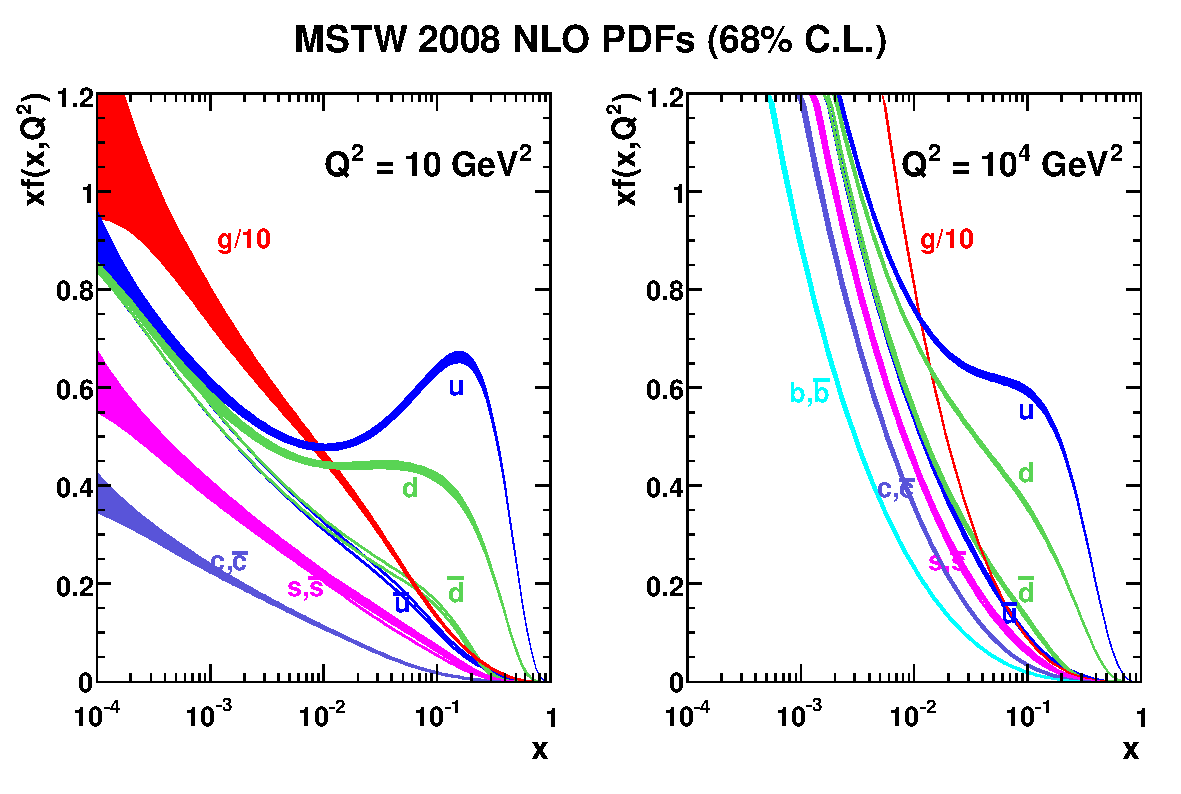
\includegraphics[width=0.9\textwidth]{images/pdfs.pdf}
  \caption{Typical momentum fraction distributions of partons inside the proton at a factorisation scale of \(Q^2 = 10\,\text{GeV}^2\) (left) and \(Q^2 = 10\,\text{GeV}^2\) (right). The plot shows the gluon and the first two generations of quarks, including valence $up$-quark and $down$-quark components~\cite{Martin_2009}.}
  \label{fig:pdfs}
\end{figure}

\subsubsection*{Parton-parton scattering}
\label{subsubsec:proton}
From these principles, the production cross-sections for the processes that unfold at hadron colliders can be factorized into two contributions. The PDFs describe the colliding partons $a$, $b$, within the colliding hadrons $H_{A}$, $H_{B}$. In the collision, the hard scattering process of interest corresponds to the short-distance interaction between both partons, each carrying a fraction of the parent hadrons's momentum. These interactions are characterised by a large momentum transfer and are described within the framework of perturbative QCD. However, the collision environment also includes soft interactions with low momentum transfer, collectively referred to as the underlying event (UE), which encompasses remnants of the hadron-hadron system as well as potential multi-parton interactions (MPI), which are cases where more than one partonic interaction occurs within a single event.

Radiative processes such as Bremsstrahlung are inherent to high-energy collisions due to the acceleration of colour and electric charges. Initial State Radiation (ISR) arises from the incoming partons before the hard interaction, while Final State Radiation (FSR) originates from the outgoing partons. Following the hard interaction, partons undergo hadronisation, a non-perturbative QCD process in which coloured partons are confined into colour-singlet hadrons. These hadrons are typically collimated into jets, observable in the detector.

Hence, the total production cross-section for a given final state $X$ in a $pp$ collision is obtained via the factorisation theorem~\cite{fact_them,collins2004factorizationhardprocessesqcd}:
\begin{equation}
\sigma_{AB \to X} = \sum_{a,b} \int \mathrm{d}x_a \, \mathrm{d}x_b \, f_{a/A}(x_a, \mu_F^2) \, f_{b/B}(x_b, \mu_F^2) \, \hat{\sigma}_{ab \to X}(\hat{s}, \mu_R^2),
\end{equation}
where $f_{a/A}$ and $f_{b/B}$ are the PDFs containing the non-perturbative component of the soft interaction, $\mu_F$ is the factorisation scale, and $\mu_R$ the renormalisation scale associated with the running of $\alpha_s$. The partonic production cross-section $\hat{\sigma}$ is computed as a perturbative expansion in $\alpha_s(\mu_R)$:
\begin{equation}
\hat{\sigma}_{ab \to X} = \hat{\sigma}_0 + \alpha_s(\mu_R^2)\, \hat{\sigma}_1 + \alpha_s^2(\mu_R^2)\, \hat{\sigma}_2 + \cdots.
\label{running}
\end{equation}

While leading order (LO) calculations offer basic estimates, they suffer from large theoretical uncertainties due to strong dependence on $\mu_F$ and $\mu_R$. Higher-order corrections at next-to leading order (NLO) or next-to-next-to leading order (NNLO) reduce this dependence and yield more accurate predictions. The impact of these corrections is often quantified via the $K$-factor, defined as the ratio of the production cross-sections computed at higher orders in QCD with respect to the LO cross-section.

%----------------------------------------------
\subsection{Electroweak Theory and Gauge Unification}
\label{subsec:ew_theory}
%----------------------------------------------

The electroweak (EW) theory unifies the weak and electromagnetic interactions within a single gauge framework. It is formulated as a non-Abelian gauge theory based on the symmetry group $SU(2)_L \times U(1)_Y$, where $SU(2)_L$ accounts for weak isospin and $U(1)_Y$ for weak hypercharge. The theory was developed independently by Glashow, Weinberg, and Salam~\cite{Glashow,Weinberg,Salam}, and constitutes a central component of the SM. The electroweak Lagrangian can be written as:

\begin{equation}
\begin{split}
\mathcal{L}_{\text{EW}} = 
&\sum_{flavours} i(\bar{L}\gamma^\mu D_\mu L +\bar{Q}\gamma^\mu D_\mu Q + \bar{l}_{R}\gamma^\mu D_\mu l_{R} + \bar{u}_{R}\gamma^\mu D_\mu u_{R} + \bar{d}_{R}\gamma^\mu D_\mu d_{R}) \\
&- \frac{1}{4} W_{\mu\nu}^a W^{a\,\mu\nu} - \frac{1}{4} B_{\mu\nu} B^{\mu\nu}
\end{split}
\label{eq:ew_lagrangian}
\end{equation}

The gauge fields associated with $SU(2)_L$ are denoted by $\vec{W}_\mu = (W_\mu^1, W_\mu^2, W_\mu^3)$, while the gauge field corresponding to $U(1)_Y$ is $B_\mu$. The corresponding gauge couplings are $g$ and $g'$, respectively. The covariant derivative acting on fermion fields is given by:
\begin{equation}
D_\mu = \partial_\mu - i \, g \, \frac{\vec{\tau}}{2} \cdot \vec{W}_\mu - i \, g' \, \frac{Y}{2} B_\mu,
\end{equation}
where $\vec{\tau}$ are the Pauli matrices and $Y$ is the weak hypercharge of the field.

Left-handed fermions are arranged in $SU(2)_L$ doublets, while right-handed fermions transform as singlets. For instance, the first-generation leptons are written as:
\begin{equation}
L_e =
\begin{pmatrix}
\nu_e \\
e
\end{pmatrix}_L, \qquad e_R,
\end{equation}
with $L_e$ transforming as a doublet under $SU(2)_L$ and $e_R$ as a singlet. It similarly applies to left-handed quark doublets, $Q$, and singlets, $u$ and $d$. The weak hypercharges are assigned such that the electric charge $Q$ of each field is given by the Gell-Mann–Nishijima relation:
\begin{equation}
Q = T_3 + \frac{Y}{2},
\end{equation}
where $T_3$ is the third component of weak isospin.

The kinetic term of the gauge fields is given by:
\begin{equation}
\mathcal{L}_{\text{gauge}} = -\frac{1}{4} \, \vec{W}_{\mu\nu} \cdot \vec{W}^{\mu\nu} - \frac{1}{4} \, B_{\mu\nu} B^{\mu\nu},
\end{equation}
where the field strength tensors are defined as:
\begin{align}
W_{\mu\nu}^i &= \partial_\mu W_\nu^i - \partial_\nu W_\mu^i + g \, \epsilon^{ijk} W_\mu^j W_\nu^k, \\
B_{\mu\nu} &= \partial_\mu B_\nu - \partial_\nu B_\mu.
\end{align}

Fermion interactions with the gauge bosons arise from the kinetic term of the fermion fields:
\begin{equation}
\mathcal{L}_{\text{fermion}} = \sum_{\psi} \bar{\psi} \, i \slashed{D} \, \psi,
\end{equation}
leading to charged and neutral current interactions. The charged currents couple only to left-handed fermions via $W^\pm$ bosons (linear combinations of $W^1$ and $W^2$), while neutral currents arise from couplings to $W^3$ and $B$.

At this stage, all gauge bosons and fermions are massless. Mass terms are forbidden by gauge invariance, and it is only through spontaneous symmetry breaking that physical masses are generated, as discussed in Section~\ref{subsec:higgs_mech}. Additionally, the structure of the theory prior to breaking ensures parity violation in weak interactions due to the chiral nature of the $SU(2)_L$ coupling.

This unbroken EW theory thus describes the fundamental structure of weak and electromagnetic interactions prior to the introduction of the Higgs field, which provides masses to the gauge bosons and fermions while preserving gauge invariance through the Higgs mechanism.

%----------------------------------------------
\subsection{Spontaneous Symmetry Breaking and the Higgs Mechanism}
\label{subsec:higgs_mech}
%----------------------------------------------

In order to generate the mass of weak vector bosons and fermions while preserving renormalizability and unitarity, the SM introduces a Spontaneous Symmetry Breaking mechanism in the electroweak theory. 
This mechanism is referred to as the Brout–Englert–Higgs (BEH) mechanism~\cite{Brout,HiggsSpontan}, and it introduces a complex scalar field doublet $\phi$ with hypercharge $Y=+1$, whose dynamics are governed by the gauge-invariant Lagrangian:
\begin{equation}
\mathcal{L}_\phi = (D_\mu \phi)^\dagger(D^\mu \phi) - V(\phi),
\end{equation}
where $V(\phi)$ is the scalar potential:
\begin{equation}
V(\phi) = \mu^2 \phi^\dagger \phi + \lambda(\phi^\dagger \phi)^2,
\label{eq:higgs_potential}
\end{equation}
with $\lambda > 0$ ensuring the potential is bounded from below. The sign of $\mu^2$ determines the nature of the vacuum: for $\mu^2 > 0$, the potential has a single minimum at $\phi = 0$, preserving the gauge symmetry. However, for $\mu^2 < 0$, the potential takes the shape of a “Mexican hat”, as illustrated in Figure~\ref{fig:mexican_hat}, with a continuous set of degenerate minima.

Since the Lagrangian is gauge invariant, the Higgs field can be described using an exponential decomposition:
\begin{equation}
\phi(x) = \frac{1}{\sqrt{2}} \, e^{i \tau_{a} \theta^a(x)/f} \begin{pmatrix}
0 \\
\rho(x)
\end{pmatrix},
\label{eq:higgs_param}
\end{equation}
where $\theta^a(x)$ and $\rho(x)$ are real fields, $\tau_{a}$ are the SU(2) generators\footnote{Elements of the group that generate the group when combined with themselves using the group's operations}, and $f$ is a normalisation constant.

One of the degenerate minima can be chosen without loss of generality as:
\begin{equation}
\langle \phi \rangle = \frac{1}{\sqrt{2}} \begin{pmatrix}
0 \\
v
\end{pmatrix},
\end{equation}
which spontaneously breaks the $SU(2)_L \times U(1)_Y$ gauge symmetry down to the electromagnetic subgroup $U(1)_{\text{EM}}$.

\begin{figure}[htbp]
  \centering
  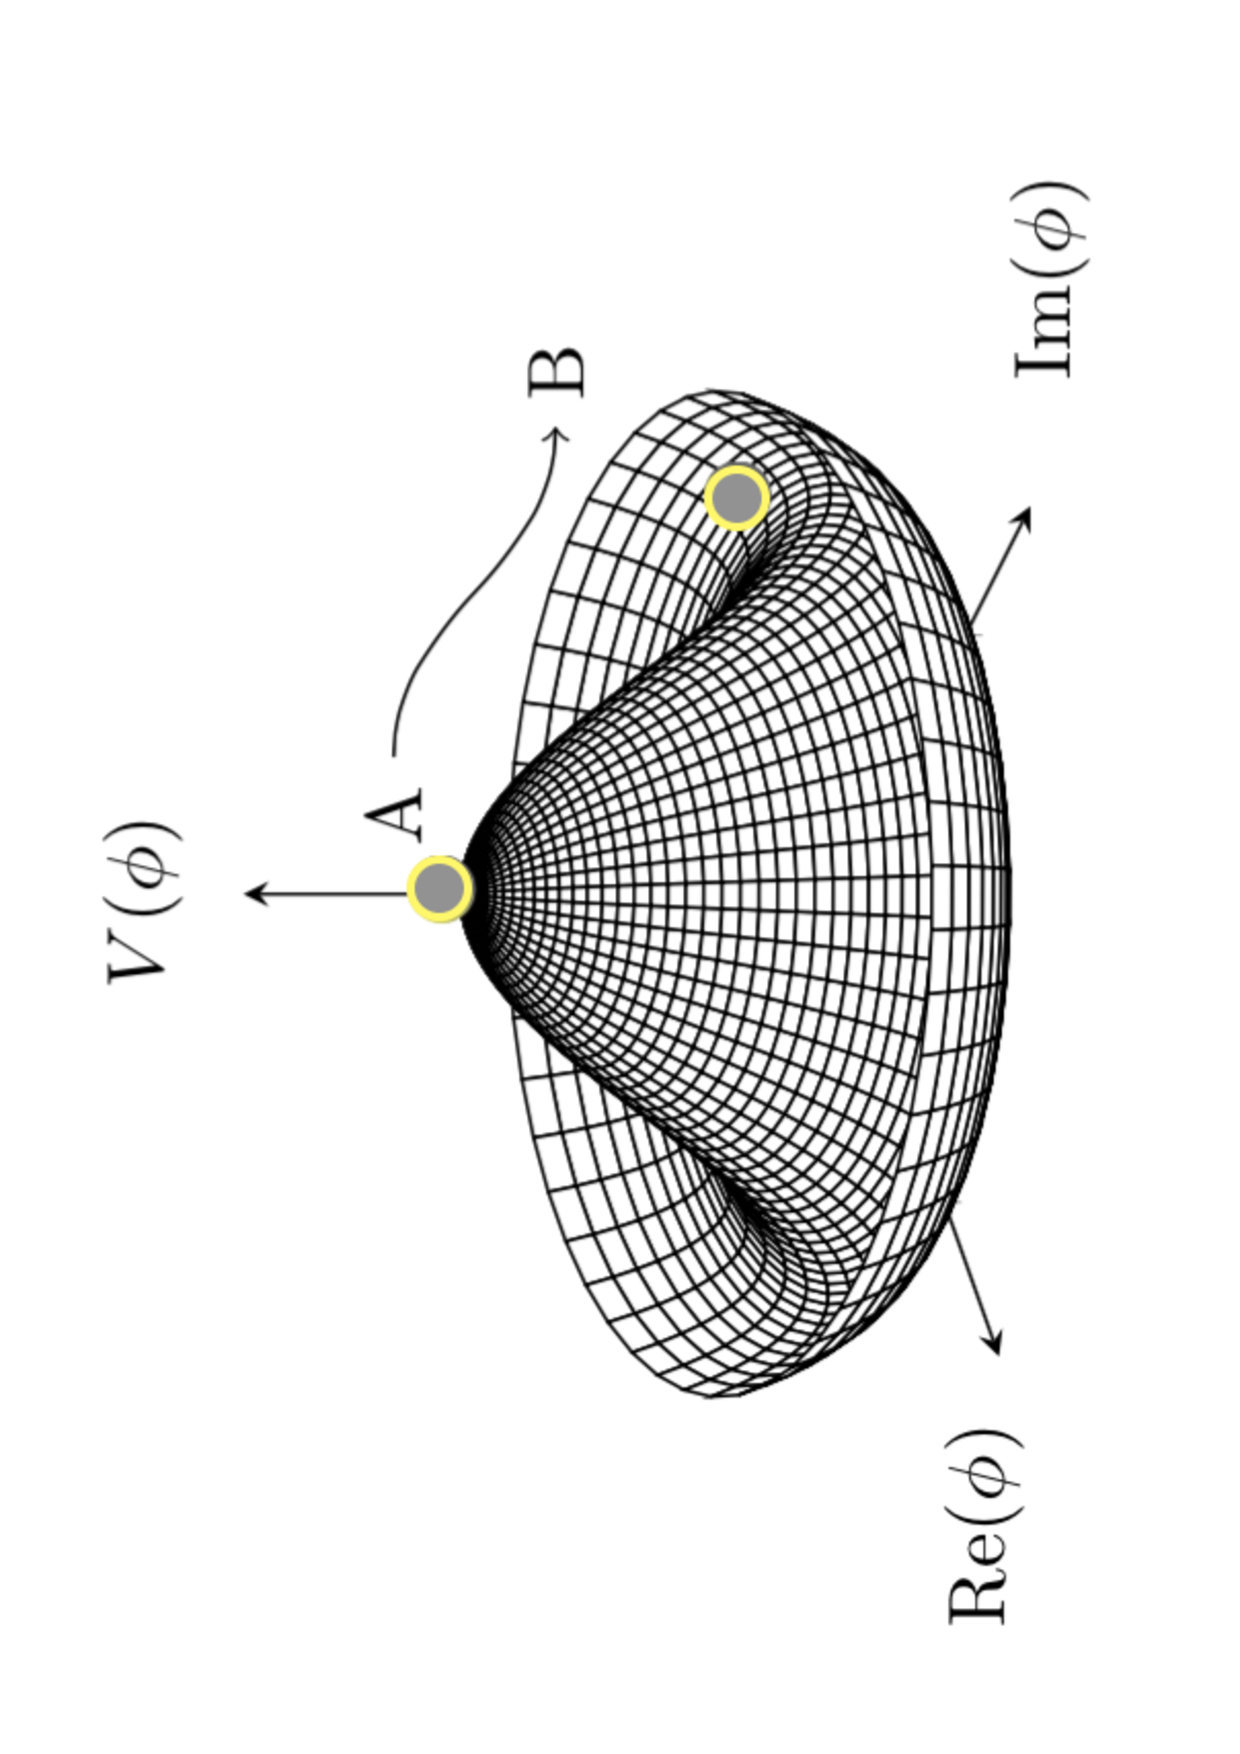
\includegraphics[angle=-90,width=0.7\textwidth]{images/mexican_hat.pdf}
  \caption{Illustration of the shape of the Higgs complex scalar potential with vacuum expectation value $v$. The symmetry is spontaneously broken when a singular ground state is chosen (A $\rightarrow$ B).}
  \label{fig:mexican_hat}
\end{figure}

The simplest way to expand the Higgs field is to keep the minimum number of degrees of freedom, so replacing $v\rightarrow v+h(x)$ in the previous equation and substituing in the potential Lagrangian (Eq.~\ref{eq:higgs_potential}): 
\begin{equation}
\begin{split}
\mathcal{L}_{H} = 
&\frac{1}{2}(\partial_{\mu}h)(\partial^{\mu}h) + \frac{1}{2}(2\mu^2)h^2\\  
& + \frac{1}{2}\frac{g^2_{W}v^2}{4}(W_{\mu}^1W^{1\mu}+W_{\mu}^2W^{2\mu})\\
& +\frac{1}{8}v^2(g_{W}W^{3\mu}-g_{B}B^{\mu})\\ 
& + \mathcal{O}(h^2)
\end{split} 
\label{eq:ew_broken}
\end{equation}

This expression contains quadratic terms interpreted as the mass terms of the particles associated to the fields. Since gauge boson terms here are not linearly independent, they cannot be interpreted as observables. Physical bosons can be obtained diagonalizing this sector, resulting in:
\begin{align}
W^\pm_\mu &= \frac{1}{\sqrt{2}} \left( W^1_\mu \mp i W^2_\mu \right), \\
Z_\mu &= \cos\theta_W W^3_\mu - \sin\theta_W B_\mu, \\
A_\mu &= \sin\theta_W W^3_\mu + \cos\theta_W B_\mu,
\end{align}
where $\theta_W$ is the weak mixing angle defined by $\tan \theta_W = g_B /g_W$.
Using these definitions, the corresponding masses of the gauge bosons can be obtained from the Lagrangian as follows:
\begin{align}
m^{\pm}_W &= \frac{1}{2} g v, \\
m_Z &= \frac{1}{2} \sqrt{g^2 + g'^2} \, v, \\
m_\gamma &= 0,
\end{align}
where $v = 246 \text{  GeV}$ is the Higgs field vacuum expectation value and $g$ is the weak isospin coupling constant. 
This mechanism results in two massive vector bosons $W^{\pm}$ which corresponds to the weak charged current, and other massive boson $Z$, carrier of the neutral weak current. It also remains a massless gauge boson, $A_{\mu}$, which corresponds to the photon and is consistent with the unbroken QED symmetry $U(1)$.

From Eq.~\ref{eq:ew_broken}, the mass term for the scalar field $H$ turns to be:
\begin{equation}
m_H^2 = 2 \mu^2,
\end{equation}
where it depends on the free parameter $\mu^2$, that can be experimentally measured, and it has been found to be close to $125$~GeV.
Actually, this Lagrangian can also be expressed in the following way after the spontaneous symmetry breaking: 
\begin{align}
\mathcal{L}_{H} &= m_W^2 W^-_{\mu} W^{+\mu} \left( 1 + \frac{h}{v} \right)^2
+ \frac{1}{2} m_Z^2 Z_{\mu} Z^{\mu} \left( 1 + \frac{h}{v} \right)^2 \notag \\
&\quad + \frac{1}{2} (\partial_{\mu} h)^2 - V(h).
\label{allterms}
\end{align}
with
\begin{equation}
    V(h) = -\frac{\mu^{4}}{4\lambda} - \mu^2h^2 + \lambda v h^3 + \frac{\lambda}{4}h^4
\label{hcoupl}
\end{equation}
where apart from the aforementioned mass term for the Higgs field, this equation also contains the Higgs self-interaction terms $h^3$ and $h^4$. 

Moreover, the BEH mechanism can also be used to provide mass terms for the fermions preserving the gauge invariance of the theory.
Adding the Yukawa terms~\cite{Peskin} describing fermion couplings to the Higgs field into the EW Lagrangian, one gets:
\begin{equation}
\mathcal{L}_{\text{Yukawa}} = 
\sum_{\text{flavours}} \left( 
- \lambda_\ell \, \bar{L} \phi \ell_R 
- \lambda_d \, \bar{Q} \phi d_R 
- \lambda_u \, \epsilon^{ab} \, \bar{Q}_a \phi_b^{\dagger} u_R 
+ \text{h.c.} 
\right)
\end{equation}
where $\lambda_{e}$, $\lambda_{d}$ and $\lambda_{u}$ are arbitrary parameters and $\epsilon^{ab}$ is the two dimensional total anti-symmetric tensor with $\epsilon^{12}=1$. After symmetry breaking we get the following mass terms for the fermion fields after proper diagonialization: 
\begin{equation}
m_{\ell}=\lambda_{\ell}\frac{v}{\sqrt{2}}, \ m_{d}=\lambda_{d}\frac{v}{\sqrt{2}}, \ m_{u}=\lambda_{u}\frac{v}{\sqrt{2}},
\end{equation}
from where the Yukawa coupling strength of fermions to the Higgs field can be defined as
\begin{equation}
\label{yukawa}
y_{f}=\sqrt{2}\frac{m_{f}}{v}
\end{equation}
Moreover, these fermion mass eigenstates and the weak eigenstates are related via the $3\times3$ unitary Cabibbo-Kobayashi-Maskawa (CKM) matrix, $V_{CKM}$,
\begin{equation}
\begin{pmatrix}
d^0 \\
s^0 \\
b^0
\end{pmatrix}
= V_{\text{CKM}}
\begin{pmatrix}
d \\
s \\
b
\end{pmatrix}
=\begin{pmatrix}
V_{ud} & V_{us} & V_{ub} \\
V_{cd} & V_{cs} & V_{cb} \\
V_{td} & V_{ts} & V_{tb}
\end{pmatrix}
\begin{pmatrix}
d \\
s \\
b
\end{pmatrix},
\end{equation}
where the off-diagonal elements cause flavour changing weak charged current interactions of quarks with their transition probabilities being proportional to $|V_{nm}|^2$.

%++++++++++++++++++++++++++++++++++++++++++++++
\section{Success and limitations of the SM}
\label{sec:BSM}
%++++++++++++++++++++++++++++++++++++++++++++++
After integrating all the essential elements forming the SM, the theory is characterized by 19 undetermined parameters:
\begin{itemize}
  \item a total of nine Yukawa couplings corresponding to the three charged leptons and six quarks;
  \item three gauge coupling constants governing the strengths of the interactions: \( g_s \), \( g \), and \( g' \);
  \item two parameters characterizing the Higgs potential: the vacuum expectation value \(\nu\) and the Higgs boson mass \(m_H\);
  \item four resulting mixing angles defining the structure of the CKM matrix;
  \item a single strong $CP$-violating phase \(\theta_{CP}\), which is conventionally assumed to be zero, implying the absence of $CP$ violation in strong interactions.
\end{itemize}
Despite being defined by 19 free parameters, the SM has demonstrated extraordinary predictive power, with theoretical predictions consistently matching experimental results over several decades. This success is exemplified in Figure~\ref{fig:totalxsect}, which presents the production cross-sections measured by the ATLAS experiment for a variety of processes occurring across multiple orders of magnitude.
\begin{figure}[htbp]
  \centering
  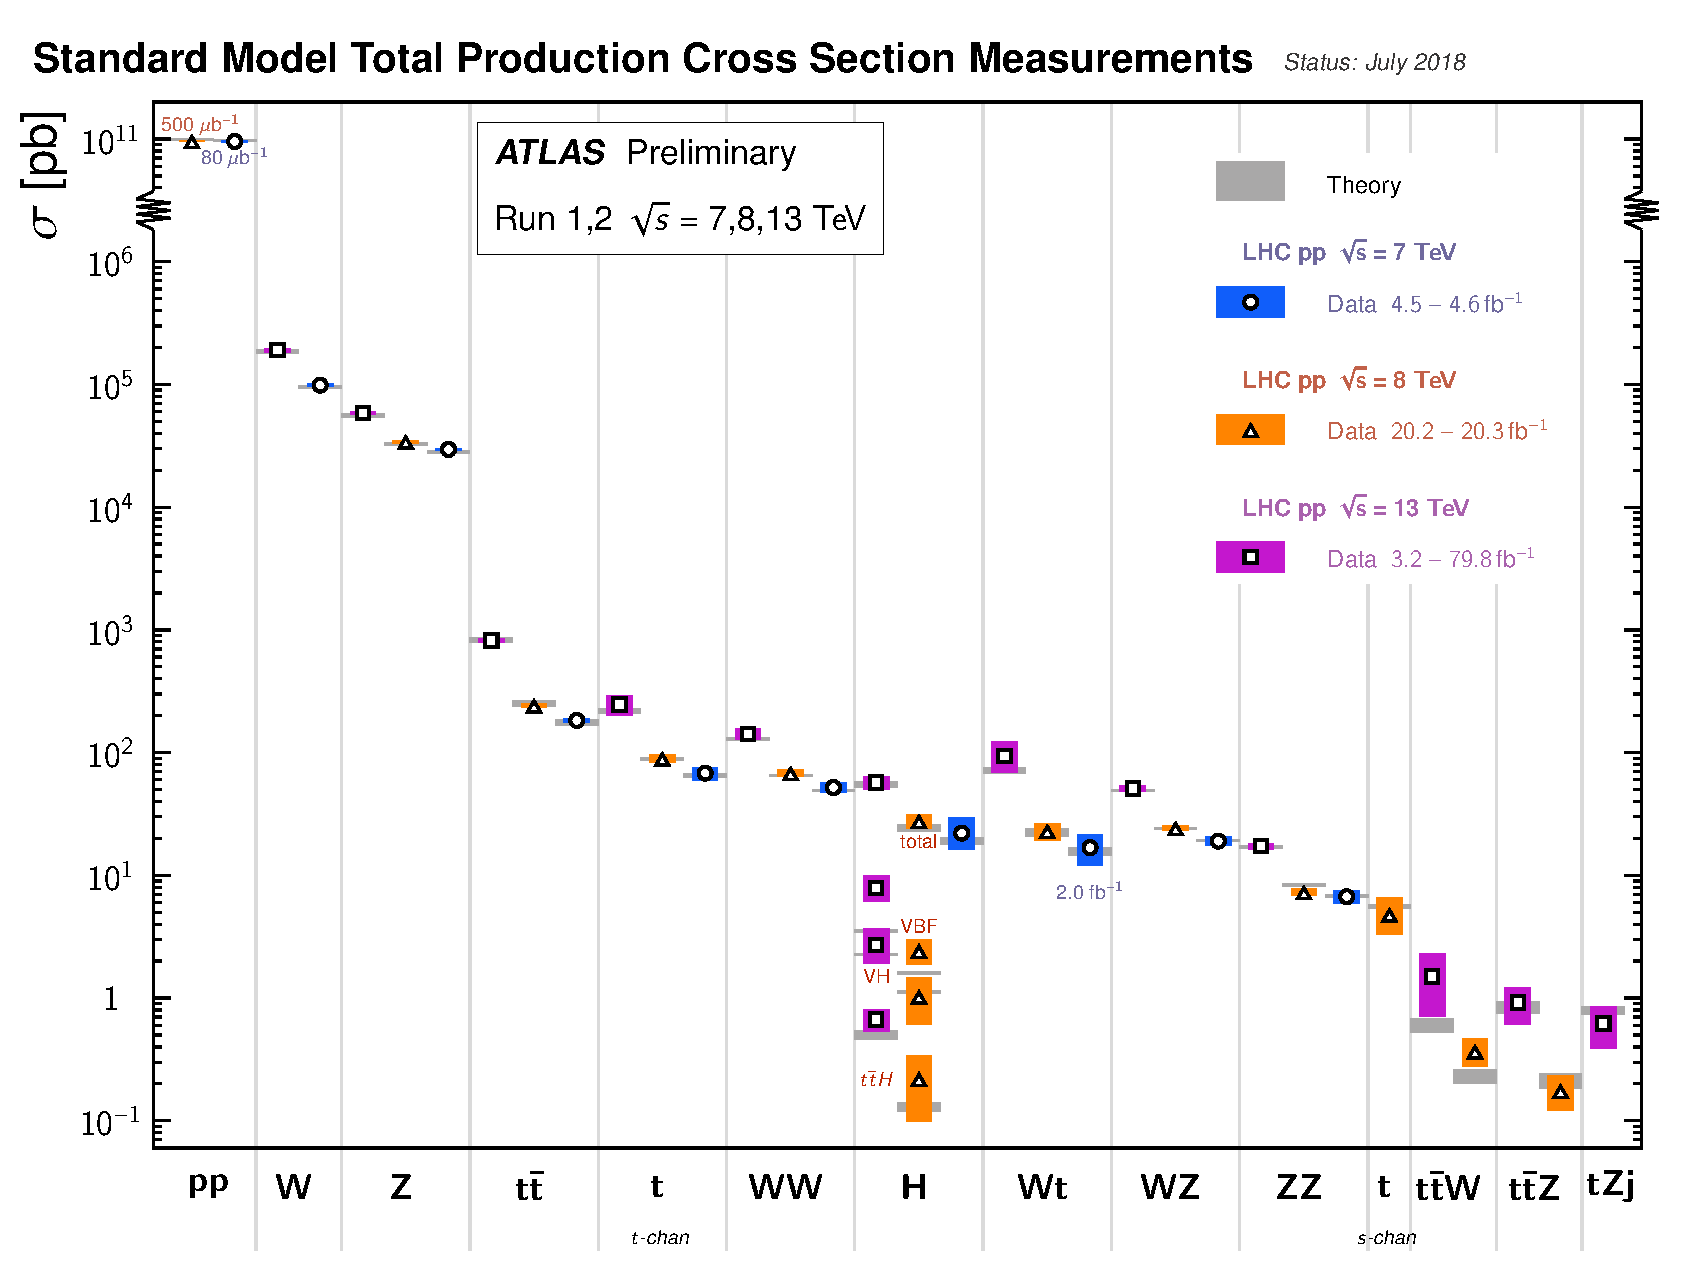
\includegraphics[width=0.8\textwidth]{images/totalxsect.pdf}
  \caption{Summary of several SM total production cross-section measurements, compared to the corresponding theoretical expectations. All theoretical expectations were calculated at NLO or higher~\cite{ATL-PHYS-PUB-2024-011}.}
  \label{fig:totalxsect}
\end{figure}

Despite its remarkable success, the SM is not considered a complete theory of fundamental interactions. Some of the most relevant issues not addressed by this theory are:
\subsubsection*{Dark Matter}

Astrophysical and cosmological observations provide compelling evidence for the existence of dark matter (DM), a form of non-luminous matter not accounted for in the SM. Measurements of galactic rotation curves, gravitational lensing in galaxy clusters (e.g., the Bullet Cluster~\cite{Clowe_2006}), and the cosmic microwave background anisotropies consistently indicate that approximately 85\% of the matter content of the universe is non-baryonic~\cite{Planck}. While several extensions of the SM propose viable DM candidates, such as weakly interacting massive particles or axions, the SM itself does not provide a suitable particle to explain these phenomena.

\subsubsection*{Neutrino Masses and Oscillations}

Experimental evidence from solar, atmospheric, reactor, and accelerator neutrino experiments has firmly established that neutrinos undergo flavor oscillations, implying they have non-zero masses and mixings~\cite{PhysRevD.98.030001}. This observation requires the existence of mass terms beyond the SM original framework, which assumes massless neutrinos. Mechanisms such as the seesaw model, introducing right-handed neutrinos or Majorana mass terms, are common in theories beyond the SM (BSM), but are not present in its minimal formulation.

\subsubsection*{Matter-Antimatter Asymmetry}

The observed universe is dominated by matter over antimatter, a phenomenon known as baryon asymmetry. While the SM includes a source of $CP$ violation through the complex phase in the CKM matrix, it is insufficient to account for the observed phenomena. Additional sources of $CP$ violation and new physics at high energy scales are required to explain this asymmetry.

\subsubsection*{Hierarchy Problem}

The mass of the Higgs boson receives large quantum corrections proportional to the square of the energy cutoff scale of the theory. Stabilizing the Higgs boson mass at the electroweak scale without unnatural fine-tuning requires a mechanism to cancel these divergences~\cite{Weinberg:1975gm,Gildener:1976ai,Weinberg:1979bn,Susskind:1978ms}. Supersymmetry~\cite{Dimopoulos:1981zb,Witten:1981nf,Dine:1981za,Dimopoulos:1981au,Sakai:1981gr,Kaul:1981hi}, composite Higgs models, and extra-dimensional theories have been proposed as potential solutions, but no evidence of such physics has been observed.

\subsubsection*{Gravity and the Lack of Unification}

The SM does not incorporate gravity, which is described by General Relativity. Moreover, the gauge couplings of the SM do not unify at a single energy scale, unless new physics is introduced. A complete theory of fundamental interactions would require a quantum theory of gravity and a framework capable of unifying all known forces, such as string theory or grand unified theories (GUTs).

\subsubsection*{Vacuum Stability and the Top-Quark Yukawa Coupling}

The stability of the EW vacuum is governed by the behaviour of the Higgs field self-coupling $\lambda$ under renormalization group (RG) evolution. In this context, the $\beta$-function encodes the scale dependence of $\lambda$ as
$\beta_\lambda \equiv d\lambda/ d \ln Q$, and determines whether the scalar potential remains stable at very high energies. At tree level, the potential in Eq.~\ref{hcoupl} is stable provided that $\lambda>0$. However, radiative corrections can alter this behaviour, driving $\lambda(Q)$ to negative values for sufficiently large $Q$. In such a case, the EW vacuum is only metastable, with a deeper minimum appearing at large field values.

Among all SM parameters, the Higgs boson mass $m_H$, the strong coupling $\alpha_s$, and especially the top-quark mass $m_t$ play the most significant roles. The value of $m_H$ sets the boundary condition for $\lambda$ at the electroweak scale, while $m_t$ determines the size of the top-quark Yukawa coupling $y_t$. Being the largest Yukawa coupling, $y_t$ provides a dominant and negative contribution to $\beta_\lambda$, effectively lowering $\lambda$ at high scales. As a consequence, the question of whether the SM vacuum is stable, metastable, or unstable is extremely sensitive to the precise value of $y_t$. Even small shifts in $m_t$ can qualitatively change the fate of the vacuum. This stability issue arises in the absence of new physics at higher energies, whereas possible effects from BSM physics could alter the running of $\lambda$ and prevent the development of such an instability.

This behaviour is illustrated in Figure~\ref{fig:vacuum_stability}. The left panel shows the full phase diagram of the SM in the $(m_t,m_H)$ plane, with regions of absolute stability, metastability, instability, and non-perturbativity. The right panel zooms into the phenomenologically relevant region around the experimentally measured values of $m_t$ and $m_H$. The figure highlights that these values lie very close to the critical boundary separating stability and metastability, suggesting that the Universe likely resides in a long-lived but metastable vacuum~\cite{Degrassi_2012}.

The importance of these considerations goes beyond a purely theoretical curiosity. Since the top-quark Yukawa coupling is the key player in determining the high-scale behaviour of $\lambda$, precision measurements of processes such as associated $t\bar{t}H$ production are essential. They not only test the SM at the electroweak scale but also probe the structure of the Higgs potential up to the Planck scale.

\begin{figure}[htbp]
    \centering
    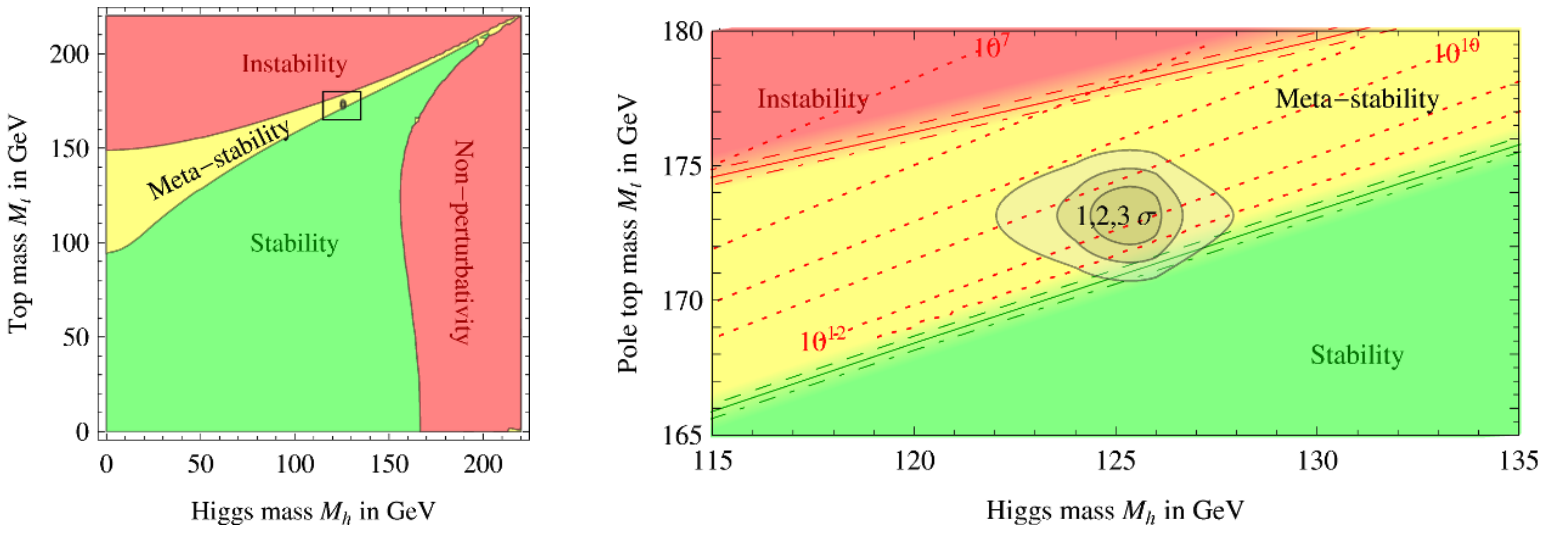
\includegraphics[width=0.9\textwidth]{images/vacuum.png}
    \caption{
        Regions of absolute stability, metastability and instability of the SM vacuum in the $(m_t, m_H)$ plane. 
        Left: full phase diagram including the region of non-perturbativity at large Higgs mass. 
        Right: zoom into the region of phenomenological interest, around the experimentally measured values of $m_t$ and $m_H$, where the Universe appears to lie close to the boundary between stability and metastability. 
        Adapted from Ref.~\cite{Degrassi_2012}.
    }
    \label{fig:vacuum_stability}
\end{figure}
%++++++++++++++++++++++++++++++++++++++++++++++
\section{Phenomenology of the Top Quark and the Higgs Boson at the LHC}
\label{sec:top_higgs_lhc}
%++++++++++++++++++++++++++++++++++++++++++++++
The top quark and the Higgs boson play a central role in the SM and in the exploration of physics beyond it. Their large masses, unique interactions, and profound implications for EWSB and vacuum stability make them particularly interesting from both theoretical and experimental perspectives. 

%xxxxxxxxxxxxxxxxxxxxxxxxxxxxxxxxxxxxxxxxxxxxxxxxxxxxxx
\subsection{The Top quark}
\label{sec:top_quark}
%xxxxxxxxxxxxxxxxxxxxxxxxxxxxxxxxxxxxxxxxxxxxxxxxxxxxxx

The top quark, initially proposed by Kobayashi and Maskawa in 1973~\cite{10.1143/PTP.49.652} and discovered at the Tevatron in 1995~\cite{PhysRevLett.74.2626,PhysRevLett.74.2632}, is the heaviest known elementary particle, with a mass of about $173$~GeV. Its extremely short lifetime causes it to decay before hadronization can occur, predominantly into a $W$ boson and a $b$ quark. Although decays into other down-type quarks are possible in principle, they are strongly suppressed by the structure of the CKM matrix and therefore negligible. Owing to its large mass, the top quark also possesses a Yukawa coupling close to unity.

\subsubsection*{Top quark production}
\label{subsec:top_quark_prod}
At hadron colliders such as the LHC, the top quark production mostly ocurrs in pairs ($t\bar{t}$) through the strong interaction. At LO, the two leading subprocesses are gluon-gluon fusion (ggF) and $q\bar{q}$ annihilation, as represented in Figure~\ref{fig:tt-production}. Gluon fusion accounts for roughly $90\%$ of the total $t\bar{t}$ production cross-section at a centre-of-mass energy of 13 TeV.
\begin{figure}[htbp]
    \centering
    \subfloat[]{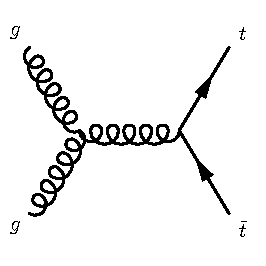
\includegraphics[width=0.3\textwidth]{feyn_gg_ttbar_1.pdf}}
    \hfill
    \subfloat[]{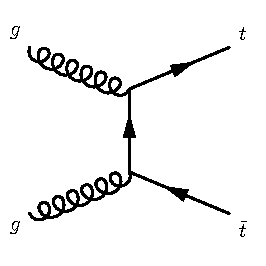
\includegraphics[width=0.3\textwidth]{feyn_gg_ttbar_2.pdf}}
    \hfill
    \subfloat[]{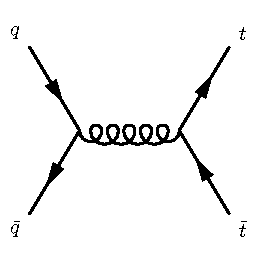
\includegraphics[width=0.3\textwidth]{feyn_qq_ttbar.pdf}}
    \caption{Leading-order Feynman diagrams contributing to top quark pair production in hadron colliders: (a) and (b) gluon-gluon fusion, which is the dominant process at the LHC, and (c) quark-antiquark annihilation, which dominates at lower center-of-mass energies such as at the Tevatron.}
    \label{fig:tt-production}
\end{figure}


Nevertheless, top quarks can also be produced singly via the electroweak interaction, either alone or in association with other particles. Single-top has a much smaller production cross-section, but processes like $tW$ or \tH encapsulate important complementary information.
Among all of them, \tH and \ttH play a central role in this thesis by forming the signal processes that are discussed in the last chapters of the thesis. They will be futher covered in more detail at the end of this chapter.

\subsubsection*{Top-antitop system decay}
\label{subsec:top_quark_decay}

Given that the top quark decays nearly the $100\%$ of cases as $t\rightarrow Wb$, the properties of $t\bar{t}$ final states mainly depend on how the $W$ boson decays, as it is shown in Figure~\ref{fig:diagram-top}.
\begin{figure}[htbp]
    \centering
    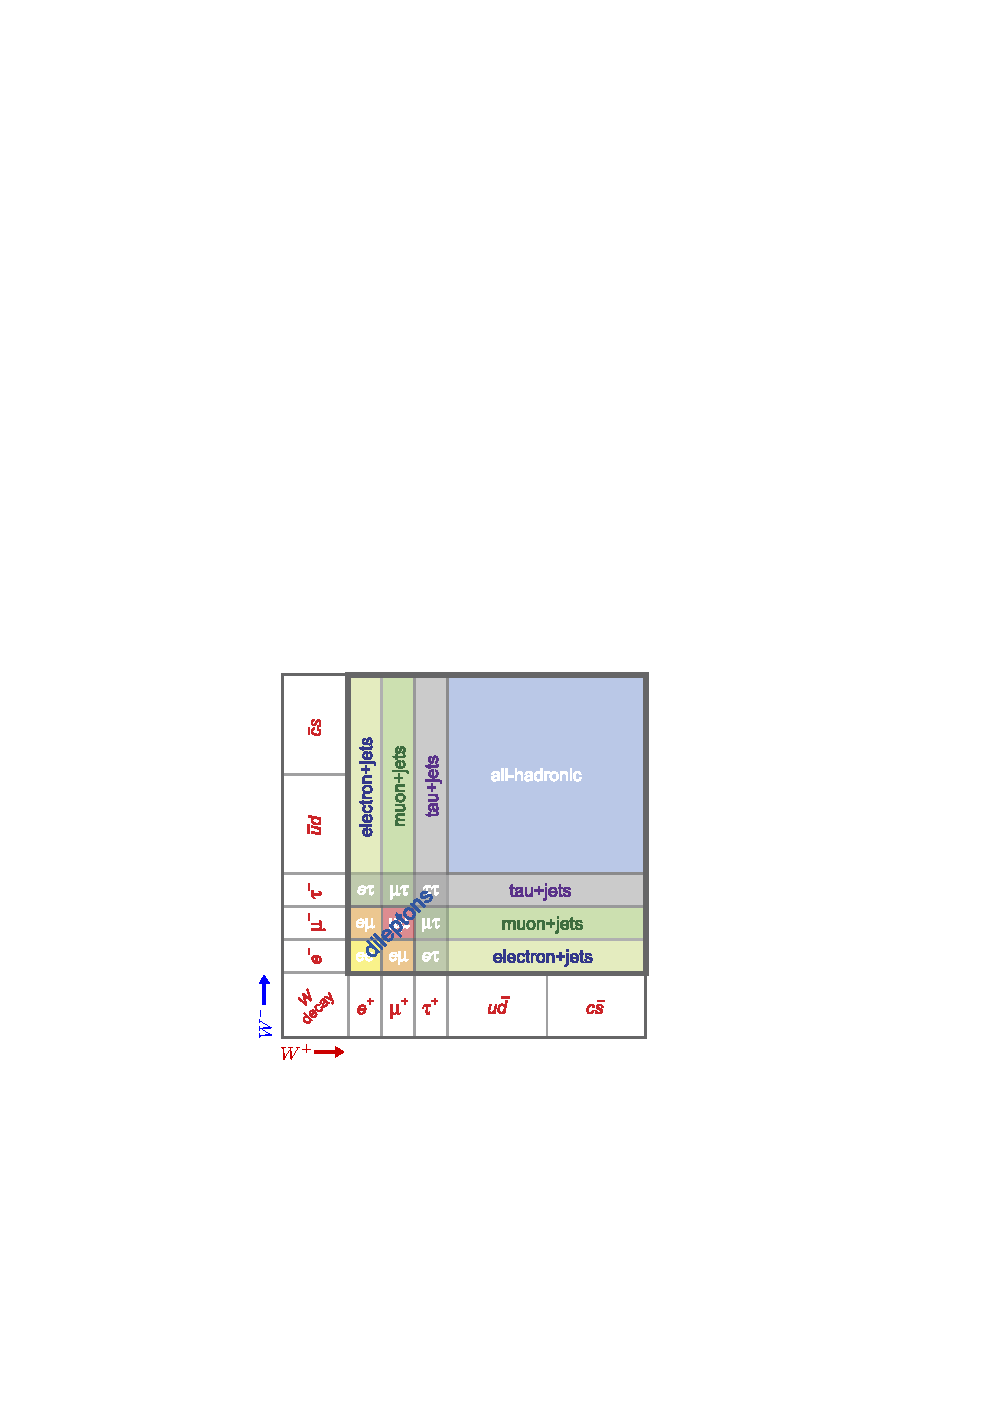
\includegraphics[width=0.5\textwidth]{tt_decay_channels.pdf}
    \caption{Classification of $t\bar{t}$ decay channels based on the $W$ decay modes~\cite{Lannon_2012}.}
    \label{fig:diagram-top}
\end{figure}

The fully hadronic final state corresponds to the case where both $W$ bosons decay into quark-antiquark pairs. This is the most frequent decay mode. An smaller fraction of events corresponds to the semileptonic final state, in which one of the bosons decays hadronically, while the other decays leptonically producing a charged lepton and a neutrino. In the case of the dileptonic final state, both $W$ bosons decay into leptons.

The table in Figure~\ref{fig:diagram-top} considers $\tau$-leptons within the general category of leptons. However, in the context of physics analysis, it is common for the term ``leptonic decay'' to be used only to refer to decays into ``light leptons'', i.e. electrons and muons, including those from the decay of $\tau$-leptons. For experimental reasons, hadronic decays of $\tau$-leptons are treated differently, as discussed in Section~\ref{sec:ttH}.

%xxxxxxxxxxxxxxxxxxxxxxxxxxxxxxxxxxxxxxxxxxxxxxxxxxxxxx
\subsection{The Higgs Boson in the LHC Physics Program}
\label{sec:higgs_program}
%xxxxxxxxxxxxxxxxxxxxxxxxxxxxxxxxxxxxxxxxxxxxxxxxxxxxxx

Since its discovery in 2012 by ATLAS and CMS~\cite{ATLAS:2012yve,CMS:2012qbp}, the Higgs boson has become a central component of the LHC physics program. Its role in providing masses to the $W$ and $Z$ bosons through the Brout–Englert–Higgs mechanism, and subsequently to all fermions in nature, is a cornerstone of the SM. Studying its properties in detail allows stringent tests of the SM and provides sensitivity to BSM scenarios.

The ATLAS and CMS experiments have undertaken a comprehensive program of Higgs boson measurements. These include the determination of its mass, spin and $CP$ properties, as well as its couplings to fermions and bosons. The precision of these measurements continues to improve with each LHC run, with new production and decay channels also being explored.

%xxxxxxxxxxxxxxxxxxxxxxxxxxxxxxxxxxxxxxxxxxxxxxxxxxxxxx
\subsubsection*{Higgs boson production mechanisms}
\label{sec:higgs_production}
%xxxxxxxxxxxxxxxxxxxxxxxxxxxxxxxxxxxxxxxxxxxxxxxxxxxxxx
The main modes at tree level in which the Higgs boson can be produced at proton-proton collisions are presented in Figure~\ref{fig:higgs_production}. Figure~\ref{fig:higgs_comb:prod} shows their respective production cross-section as a function of the centre-of-mass energy for a Higgs boson with mass $m_{H}=125$ GeV.

% Begin the figure
\begin{figure}[htbp]
    \centering
    % Primera fila: 3 imágenes centradas
    \begin{tabular}{ccc}
        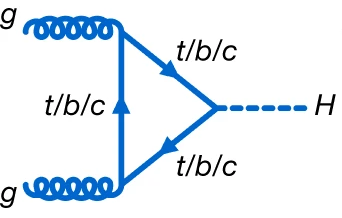
\includegraphics[width=0.3\linewidth]{images/ggF.png}  &
        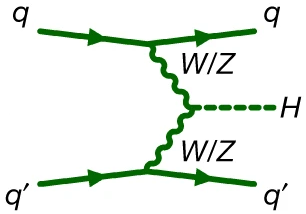
\includegraphics[width=0.3\linewidth]{images/VBF.png}  &
        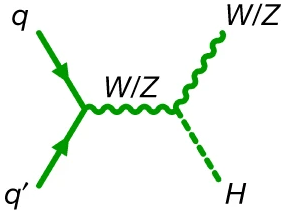
\includegraphics[width=0.3\linewidth]{images/VH.png}   \\
        (a) $ggF$ & (b) $VBF$ & (c) $VH$ \\
    \end{tabular}
    \vspace{0.5em} % Espacio entre filas
    % Segunda fila: 2 imágenes centradas bajo las 3 primeras
    \makebox[\textwidth][c]{%
        \begin{tabular}{cc}
            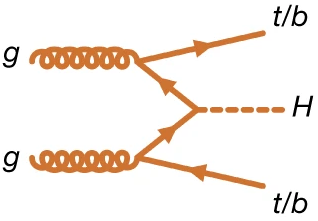
\includegraphics[width=0.3\linewidth]{images/ttH.png} &
            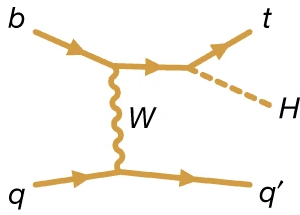
\includegraphics[width=0.3\linewidth]{images/tH.png} \\
            (d) $t\bar{t}(b\bar{b})H$ & (e) $tH$ \\
        \end{tabular}%
    }
    \caption{
    Examples of leading order Feynman diagrams for Higgs-boson production modes at the LHC~\cite{Nature_ATLAS}.}
    \label{fig:higgs_production}
\end{figure}

\begin{figure}[htbp]
    \centering
    
    \begin{subfigure}[b]{0.46\textwidth}
        \centering
        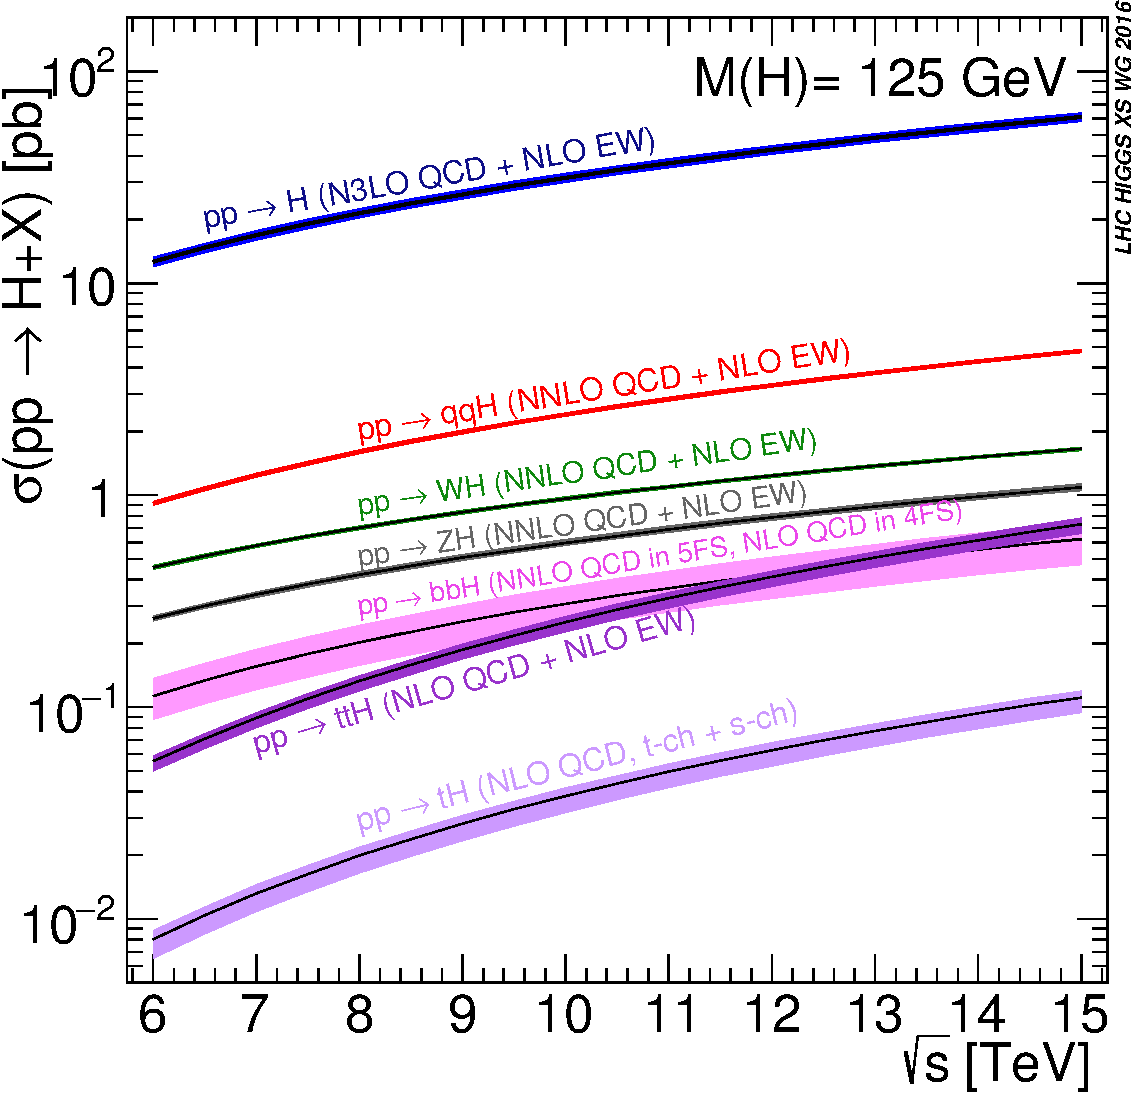
\includegraphics[width=\linewidth]{images/higgs_prod.pdf}
        \caption{}
        \label{fig:higgs_comb:prod}
    \end{subfigure}
    \hfill
    \begin{subfigure}[b]{0.46\textwidth}
        \centering
        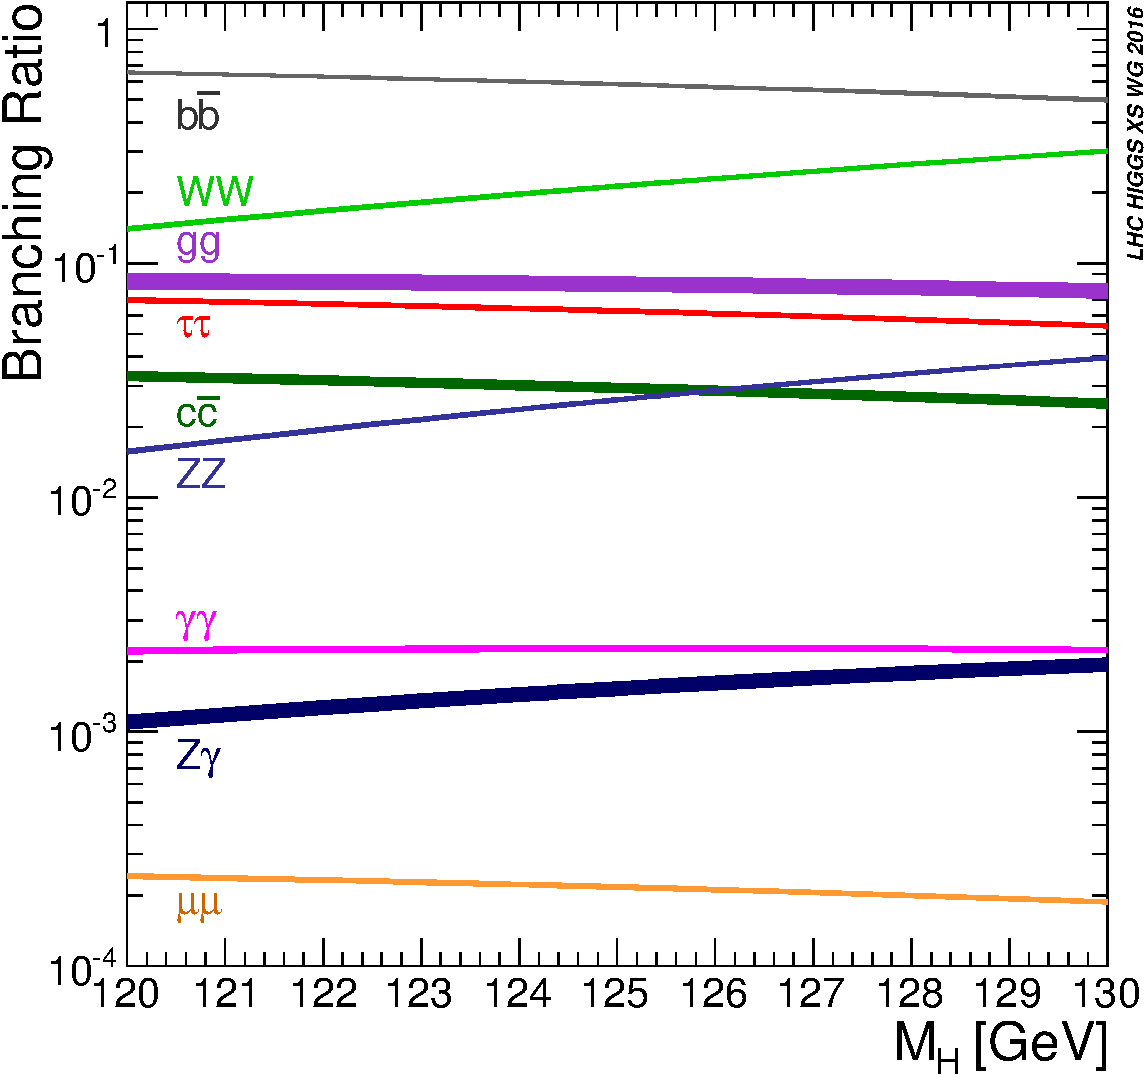
\includegraphics[width=\linewidth]{images/higgs_dec.pdf}
        \caption{}
        \label{fig:higgs_comb:dec}
    \end{subfigure}

    \caption{(a) Cross-sections measured for Higgs boson production as a function of the center of mass energy in proton-proton collisions. (b) Branching ratios for the different Higgs boson decay modes as a function of the Higgs boson mass~\cite{Nature_ATLAS}.}    \label{fig:higgs_comb}
\end{figure}



The dominant production mode is gluon-gluon fusion (ggF), where two gluons from the colliding protons interact via a heavy quark loop, primarily involving the top quark, to produce a Higgs boson. This process accounts for about 90\% of the total Higgs boson production cross-section at the LHC energies, due to the high gluon density within the proton.

Another important channel is vector boson fusion (VBF), responsible approximately $7\%$ of the total production cross-section. The Higgs boson is produced via a $t$-channel exchange of two weak bosons radiated from the incoming quarks. This mechanism is characterized by the presence of two high-momentum hard jets emitted at small angles from the colliding protons, while the Higgs boson is tipically produced between them in the central region, offering a clean and efficient experimental signature. 

Associated production with a vector boson ($VH$), where the Higgs boson is produced alongside a $W$ or $Z$ boson, is particularly useful in final states with leptons, providing strong handles for background discrimination in a hadronic environment. It provides around the $4\%$ of the Higgs boson production cross-section.

Finally, the associated production with a pair of top quarks ($t\bar{t}H$) provides a direct probe of the Yukawa coupling between the Higgs boson and the top quark, the strongest coupling in the SM. Although its production cross-section is significantly lower than other channels, around $1\%$ of the total, it plays a strategic role in testing the interaction responsible for the top-quark mass generation, which will be discussed in the following.
The rarest considered production mode is the associated production with a single top quark, accouting for approximately $0.2\%$. This process could also contribute to the direct determination of the top-quark Yukawa coupling. However, its production cross-section is significantly smaller than \( t\bar{t}H \) production. Furthermore, additional LO diagrams for $tH$ production involve the $WH$ coupling, which already blurs the measurement.

Additionally, there are other production modes that remain experimentally challenging, such as Higgs boson production in association with bottom quark pairs, \( b\bar{b}H \). While this mode has a production cross-section comparable to that of \( t\bar{t}H \), it suffers from a much less clean experimental signature due to the large background contribution from multijet production.

%xxxxxxxxxxxxxxxxxxxxxxxxxxxxxxxxxxxxxxxxxxxxxxxxxxxxxx
\subsubsection*{Higgs boson decay modes}
\label{sec:higgs_decay}
%xxxxxxxxxxxxxxxxxxxxxxxxxxxxxxxxxxxxxxxxxxxxxxxxxxxxxx

The SM Higgs boson, with a lifetime of approximately \(10^{-22}\) seconds, decays into a wide range of experimentally accessible final states that enable its observation, as its extremely short existence precludes direct detection.

As mentioned in Section~\ref{subsec:higgs_mech}, the coupling of the Higgs boson to fermions is proportional to the fermion mass, while for gauge bosons the coupling is proportional to \(m_Z^2\) and \(m_W^2\) in the \(HZZ\) and \(HWW\) vertices, respectively. Consequently, the Higgs boson decays preferentially into the heaviest particles kinematically allowed.

Figure~\ref{fig:higgs_comb:dec} shows the predicted branching ratios for the decay of the SM Higgs boson as a function of its mass. Representative Feynman diagrams for the dominant decay modes are shown in Figure~\ref{fig:h_decays}.
\begin{figure}[htbp]
    \centering
    
    % Primera fila
    \begin{subfigure}[b]{0.3\linewidth}
        \centering
        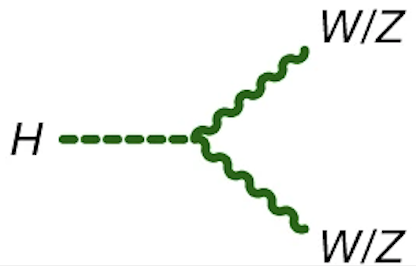
\includegraphics[width=\linewidth]{images/HVV.png}
        \caption{}
        \label{fig:h_decays:VV}
    \end{subfigure}
    \hfill
    \begin{subfigure}[b]{0.3\linewidth}
        \centering
        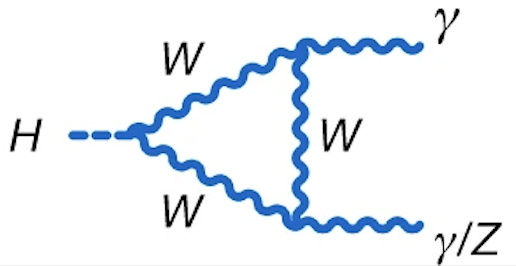
\includegraphics[width=\linewidth]{images/Hgg.png}
        \caption{}
        \label{fig:h_decays:gg}
    \end{subfigure}
    \hfill
    \begin{subfigure}[b]{0.3\linewidth}
        \centering
        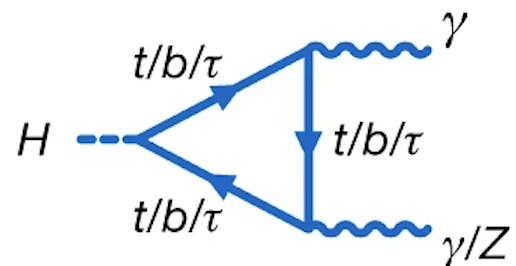
\includegraphics[width=\linewidth]{images/Hgg_loop.png}
        \caption{}
        \label{fig:h_decays:Zg}
    \end{subfigure}
    
    \vspace{0.7em} % Espacio entre filas
    
    % Segunda fila
    \begin{subfigure}[b]{0.3\linewidth}
        \centering
        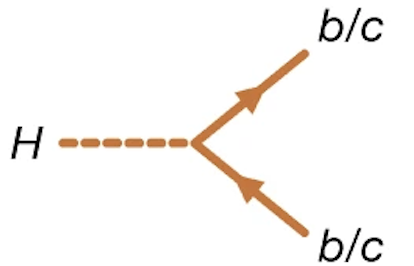
\includegraphics[width=\linewidth]{images/Hbb.png}
        \caption{}
        \label{fig:h_decays:bb}
    \end{subfigure}
    \hspace{0.1\linewidth}
    \begin{subfigure}[b]{0.3\linewidth}
        \centering
        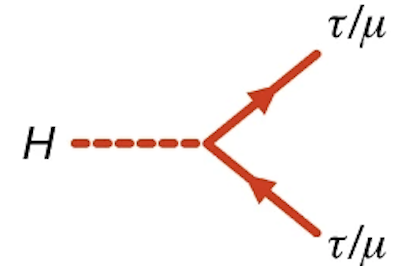
\includegraphics[width=\linewidth]{images/Htt.png}
        \caption{}
        \label{fig:h_decays:tautau}
    \end{subfigure}
    
    \caption{Representative LO Feynman diagrams for the main decay modes of a Higgs boson of 125 GeV to (a) a pair of vector bosons, (b),(c) a pair of photons or a $Z$ boson and a photon, (d) a pair of quarks, and (e) a pair of charged leptons~\cite{Nature_ATLAS}.}
    \label{fig:h_decays}
\end{figure}

The Higgs boson predominantly decays into a pair of bottom quarks, \( H \rightarrow b\bar{b} \), with a branching ratio ($\mathcal{B}$) of approximately \( \mathcal{B}(H \rightarrow b\bar{b}) \approx 0.581 \). However, the measurement of this decay mode at the LHC is challenging due to the overwhelming background from multijet production. Despite this, its large branching ratio motivates dedicated studies, especially in channels involving the associated production of a Higgs boson with a vector boson, which enhances the analysis sensitivity.

Decays into pairs of gauge bosons are suppressed, since at least one of the two bosons must be produced off-shell due to the mass of the Higgs boson. The corresponding branching ratios are approximately \( \mathcal{B}(H \rightarrow WW^*) \approx 0.22 \) and \( \mathcal{B}(H \rightarrow ZZ^*) \approx 0.03 \). Among these, the \( H \rightarrow ZZ^* \) decay mode stands out due to its clean experimental signature and high resolution, as the $Z$ bosons can decay fully leptonically into pairs of electrons or muons that are efficiently reconstructed and identified in the detector. 
In contrast, the \( H \rightarrow WW^* \) channel is experimentally more challenging: while the $W$ bosons may decay hadronically, producing jets that are difficult to distinguish from the overwhelming QCD background, their leptonic decays unavoidably involve neutrinos that escape detection, leading to missing energy and degrading the mass resolution. This makes the reconstruction of the Higgs boson in this channel substantially more difficult compared to the four-lepton final state of \( H \rightarrow ZZ^* \).

The Higgs boson can also decay into a pair of photons, \( H \rightarrow \gamma\gamma \), via a one-loop radiative process involving virtual top quarks, as can be seen in Figure~\ref{fig:h_decays:Zg}, or $W$ boson loops, as shown in Figure~\ref{fig:h_decays:gg}. Although this decay has one of the lowest branching ratios, with \( \mathcal{B}(H \rightarrow \gamma\gamma) \approx 0.227\% \), it plays a key role in Higgs boson studies at the LHC due to its excellent signal-to-background ratio. This leads to a very clean experimental signature with high resolution, especially when compared to the background from prompt photon pair production.

The decay into a pair of $\tau$-leptons is also possible for the Higgs boson, with a branching ratio of approximately \( \mathcal{B}(H \rightarrow b\bar{b}) \approx 6\% \). This decay mode plays a central role in this thesis. From the experimental point of view, the $H \rightarrow \tau\tau$ decay presents several challenges. First, the presence of neutrinos in $\tau$-lepton decays prevents a full reconstruction of the di-$\tau$ final state, complicating the determination of the Higgs boson mass. To overcome this limitation, advanced reconstruction techniques must be employed to estimate the mass of the di-$\tau$ system.

In addition, the $H \rightarrow \tau\tau$ decay is affected by a significant irreducible background from $Z \rightarrow \tau\tau$ events, whose production cross-section is several orders of magnitude larger than that of the Higgs boson. Despite these difficulties, this decay channel offers an unique opportunity to probe the Yukawa interaction between the Higgs boson and the $\tau$-lepton, providing the most precise measurement of a fermionic coupling to date due to its relatively large branching ratio. Furthermore, it allows for the study of the $CP$ properties of the Higgs boson, both in its production mechanisms and decay, and offers good sensitivity to the VBF production mode.

In the context of the Yukawa sector, the SM also predicts Higgs boson decays to fermions of the first and second generation. The decay into muons, \( H \rightarrow \mu\mu \), although having a very small branching ratio of about 0.02\%, presents a clean experimental signature with two well-reconstructed muons in the final state. However, its measurement is significantly affected by the large background from the Drell--Yan production ($Z/\gamma* \to \mu \mu$). On the other hand, the \( H \rightarrow c\bar{c} \) decay has a larger branching ratio of approximately 2.9\%, but its measurement at the LHC is challenged by the large multijet background. In addition, the identification of charm quarks remains a difficult task in the environment of a hadron collider. Decays of the Higgs boson to lighter fermions have exceedingly small branching fractions, rendering their direct observation unfeasible with current experimental sensitivity~\cite{https://doi.org/10.23731/cyrm-2017-002}.

%xxxxxxxxxxxxxxxxxxxxxxxxxxxxxxxxxxxxxxxxxxxxxxxxxxxxxx
\subsection{The \ttH process: a gateway to the Yukawa sector}
\label{sec:ttH}
%xxxxxxxxxxxxxxxxxxxxxxxxxxxxxxxxxxxxxxxxxxxxxxxxxxxxxx
As already highlighted in previous sections, the top-quark Yukawa coupling, $y_t$, is the strongest among all SM fermions, owing to the large mass of the top quark. This makes $y_t$ particularly sensitive to possible BSM contributions and an essential parameter to explore the nature of electroweak symmetry breaking~\cite{Englert:2014uua,Dobrescu:1997nm,Chivukula:1998wd,Delepine:1995qs}. Moreover, direct access to $y_t$ is crucial for probing the $CP$ structure of the Higgs sector~\cite{Bernreuther:2002uj,Brod:2013cka}, and plays an indirect role in constraining the Higgs field self-coupling~\cite{Buttazzo:2013uya,Degrassi:2016wml}.

While a direct measurement via the $H\to t\bar{t}$ decay is not accessible due to kinematic suppression due to the large mass of the top quarks, $t\bar{t}H$ offers an unique and direct probe of $y_t$. Contrary to ggF, where the coupling appears in a quantum loop that may receive BSM contributions, the \ttH process provides tree-level sensitivity to $y_t$, being the production cross-section proportional to the coupling. This complementarity is particularly useful when comparing indirect constraints from loop-induced processes to direct measurements~\cite{Ng:1983jm,Kunszt:1984ri,Beenakker:2001rj}.

The \ttH production mode was first observed in 2018 by the ATLAS and CMS collaborations~\cite{ATLAS:2018mme,CMS:2018uxb}, following the combination of multiple analyses targeting different Higgs boson decay channels. Among these channels, the $H\to b \bar{b}$ and $H\to \gamma \gamma$ analyses provided the first hints due to their high branching ratio or clean experimental signature, respectively. However, both channels come with significant limitations: the former suffers from large backgrounds with $b$-jets and sizeable modeling uncertainties, while the latter is constrained by its low branching fraction.

In addition, the so-called ``multilepton analysis'' (\ttH(ML)) constitutes another powerful probe of $t\bar{t}H$ production, targeting final states with multiple light leptons (electrons and muons) and hadronically decaying $\tau$-leptons. These signatures arise predominantly from Higgs decays into $WW^*$ or $ZZ^*$, as well as from leptonic decays of $\tau$-leptons, leading to complex final states with high lepton multiplicity. The multilepton channel benefits from relatively clean experimental signatures and good background suppression, although it is statistically limited due to the small branching fractions of these decays. Within ATLAS, the $t\bar{t}H$(ML) analysis has become one of the most sensitive channels in the overall $t\bar{t}H$ combination.

Among the Higgs boson decay modes, the $H\to\tau\tau$ channel offers an alternative strategy that strikes a balance between statistical power and experimental cleanliness. Its branching ratio is significantly larger than that of $H\to \gamma \gamma$, and although $\tau$-leptons are more challenging to reconstruct than electrons or muons, they lead to final states with relatively low backgrounds and good experimental sensitivity.

The analysis of $t\bar{t}H$ production with $H\to\tau\tau$ decays is often grouped with other multilepton channels ($H\to WW^*, ZZ^*$) due to similarities in event topology. However, the main analysis presented in this thesis focuses on the specific case where both $\tau$-leptons decay hadronically. This channel is not included within the leptonic or semileptonic categories of the $t\bar{t}H$(ML) analysis. Instead, it is treated as part of the dedicated $H\to\tau\tau$ analysis. In Chapter~\ref{chap:htautau}, the distinctive experimental signature and the potential of this process will be exploited.
%xxxxxxxxxxxxxxxxxxxxxxxxxxxxxxxxxxxxxxxxxxxxxxxxxxxxxx
\subsection{Measurements of production cross-section and branching ratios: the STXS framework}
\label{sec:stxs_yukawa}
%xxxxxxxxxxxxxxxxxxxxxxxxxxxxxxxxxxxxxxxxxxxxxxxxxxxxxx
Measurements targeting a Higgs boson signal commonly focus on determining a signal strength modifier, denoted as $\mu$. This parameter is defined as the ratio of the measured production cross-section times the branching ratio to the corresponding SM prediction:
\begin{equation}
\label{signal_strength}
    \mu = \frac{\sigma \times \mathcal{B}}{\sigma_{\mathrm{SM}} \times \mathcal{B}_{\mathrm{SM}}},
\end{equation}
where $\sigma$ denotes the production cross-section and \mathcal{B} the decay branching ratio.

Such measurements aim to maximize sensitivity to the Higgs boson signal by comparing observed event yields in data to the expected yields from the SM for each of the main Higgs boson production modes.

During the Run-2 period of the LHC, all the main Higgs boson production and decay modes have been observed with varying degrees of significance. The latest combined results from the ATLAS experiment for production cross-section and decay branching ratio measurements show a remarkable agreement with SM expectations, as illustrated in Figure~\ref{fig:higgs_mu}, resulting in a measured inclusive signal strength of $\mu = 1.05 \pm 0.06$~\cite{Nature_ATLAS}. Similar value was obtained by the CMS collaboration~\cite{CMS:2022dwd}. Evidence for rare decay modes, such as $H \to Z\gamma$ and $H \to \mu\mu$, has also been reported~\cite{Aad_2024,muon2021}.

\begin{figure}[htbp]
    \centering
    \subfloat[(a)]{
        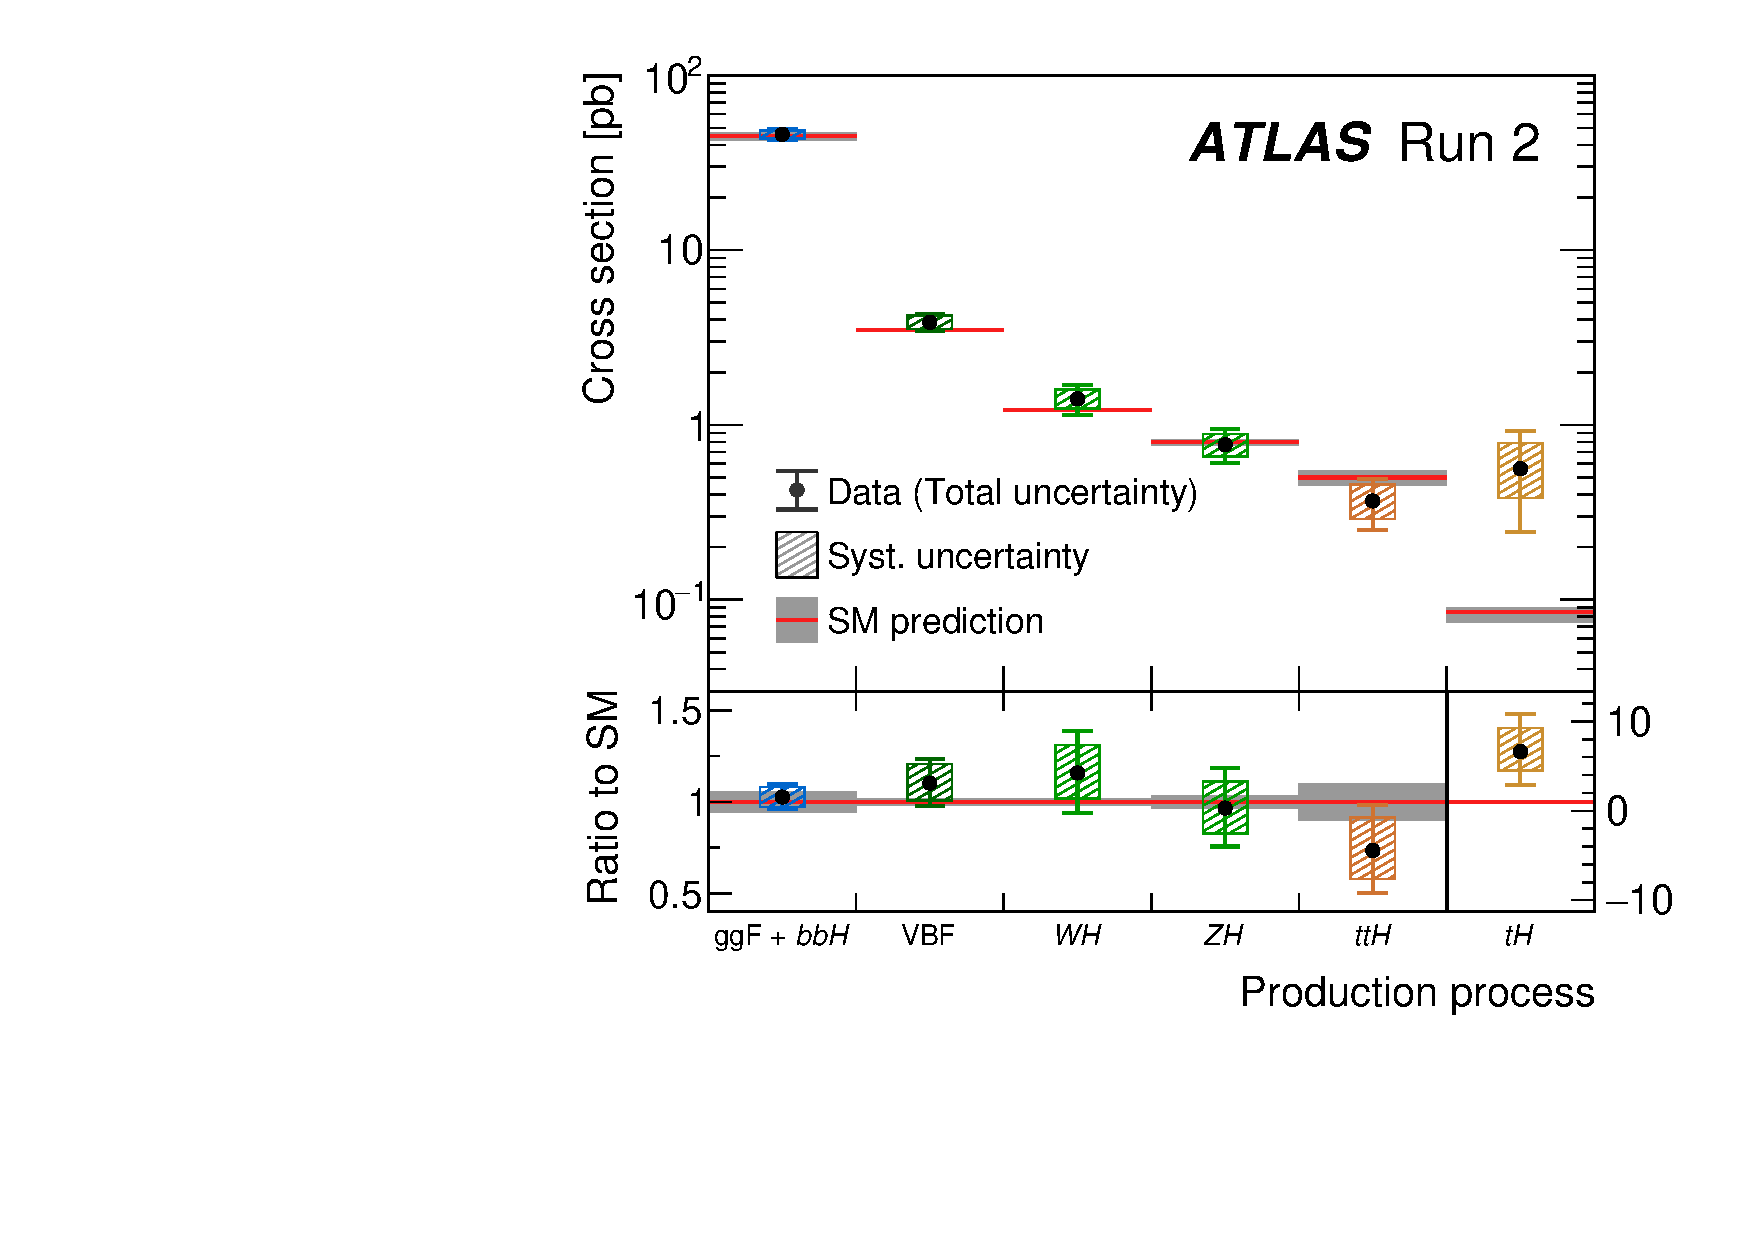
\includegraphics[width=0.46\textwidth]{atlas_combined_xsect.pdf}
    }
    \hfill
    \subfloat[(b)]{
        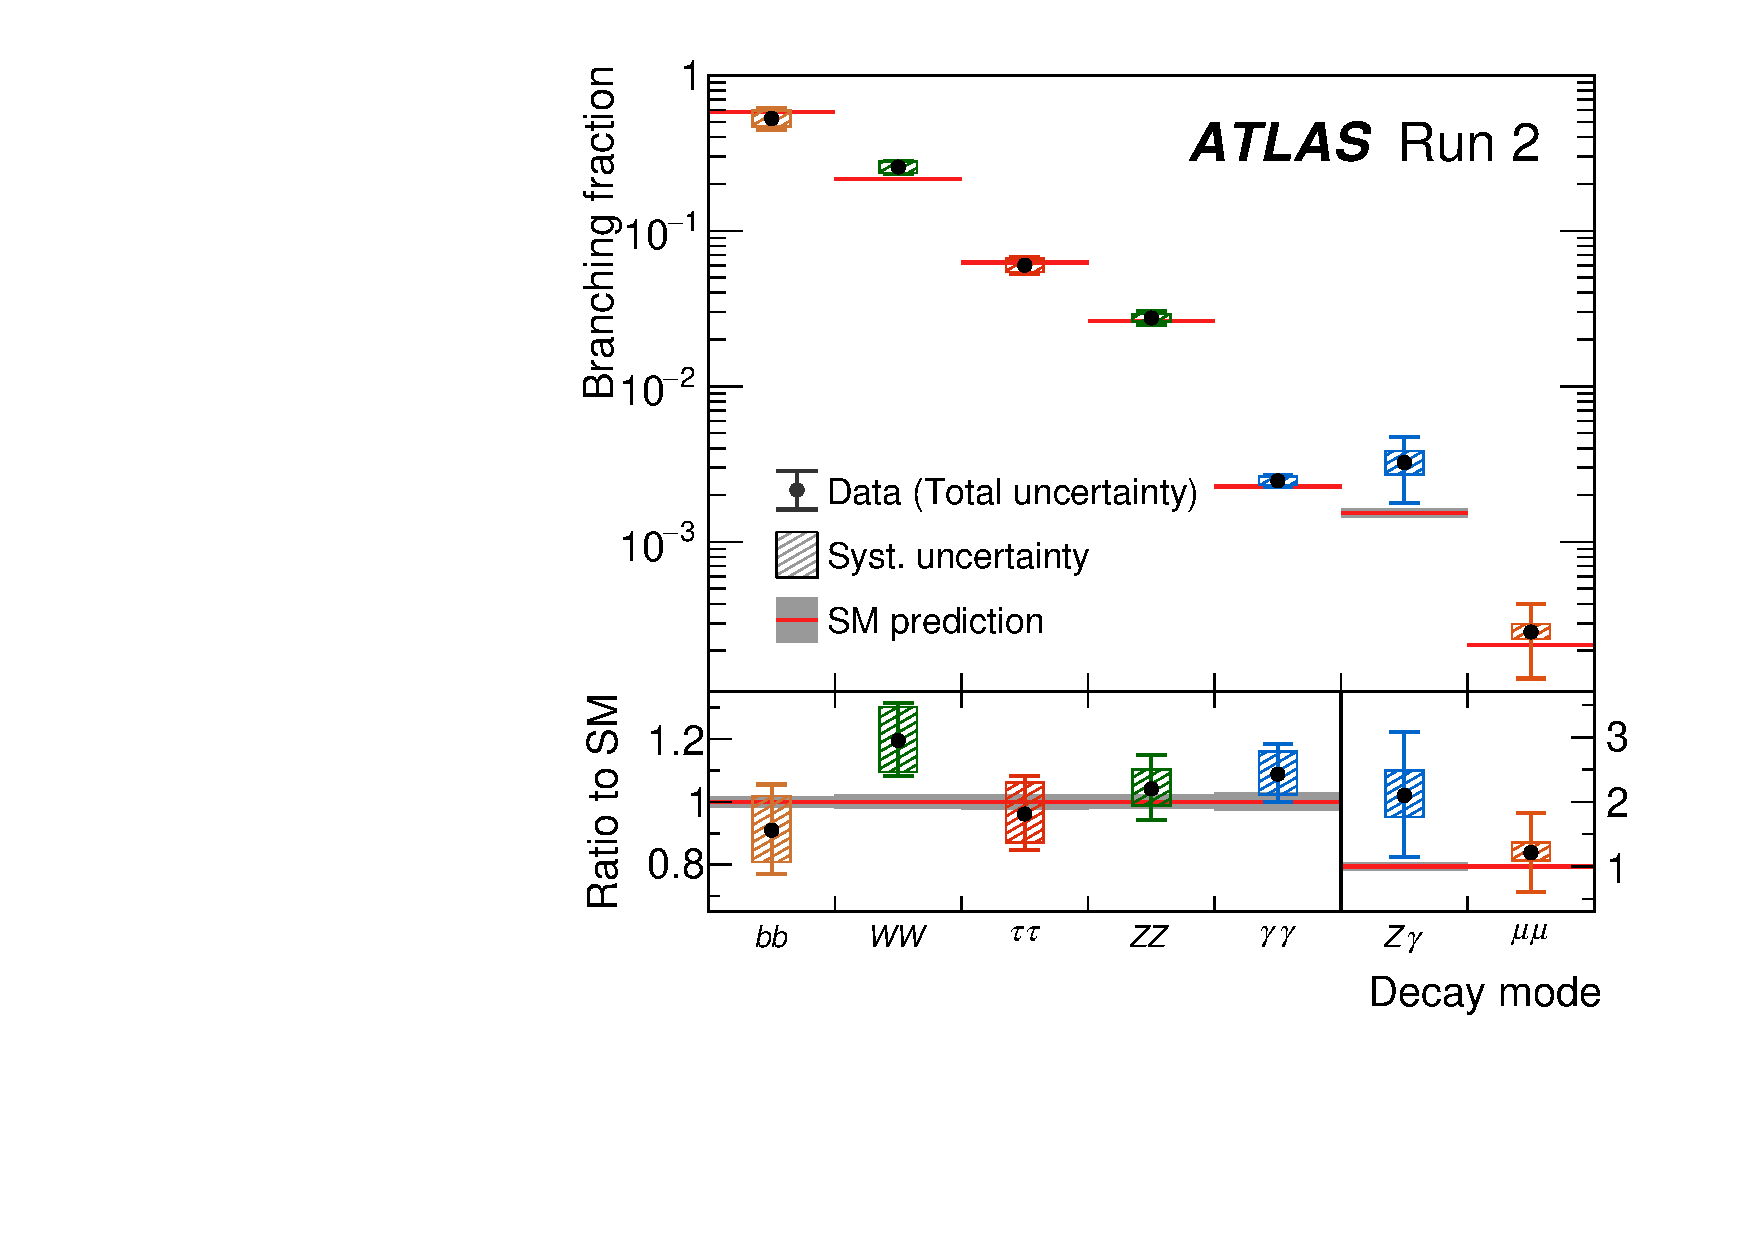
\includegraphics[width=0.46\textwidth]{atlas_combined_br.pdf}
    }
    \caption{(a) Summary of the Higgs boson production cross-sections assuming SM values for the Higgs boson branching ratios. 
    (b) Measurements of the Higgs boson decay branching ratios assuming SM predictions for the production cross-sections. 
    All results are obtained using ATLAS Run-2 data, combining different analyses, and are consistent with the SM predictions within uncertainties~\cite{Nature_ATLAS}.}
    \label{fig:higgs_mu}
\end{figure}


Despite their overall success, these inclusive measurements exhibit limited sensitivity to BSM effects that could manifest in specific phase space regions where few signal events are expected. Furthermore, these inclusive analyses depend heavily on theoretical predictions, as the uncertainty in the global signal strength $\mu$ is directly influenced by the uncertainties in the SM production cross-section and branching ratio calculations that are assumed. Additionally, analysis strategies and event selection criteria typically assume SM kinematics for the expected signal, which may reduce sensitivity to BSM scenarios.

An alternative approach to reduce the dependence on SM theoretical extrapolations is the measurement of fiducial production cross-sections. In these analyses, a fiducial phase space is defined at particle level\footnote{The particle level indicates the level in which all the physical objects are defined using stable particles in their final states, after parton shower and hadronisation, but without any interaction with the detector.}, designed to closely resemble the reconstructed event selections to minimize the extrapolation from the measured phase space. Detector effects are corrected using simulations, allowing a direct comparison of the measured fiducial production cross-section with theoretical predictions. However, the requirement of similar selections at particle and detector levels often necessitates simplified event selections, which might not be optimal for signal-to-background discrimination. The use of multivariate techniques is typically limited in fiducial measurements due to the complexity of mapping reconstructed variables to particle-level definitions.

Fiducial production cross-section measurements can be further extended to differential production cross-section measurements, where the production rates are measured as functions of relevant kinematic observables. These measurements provide richer information on the Higgs boson production dynamics and possible deviations from SM predictions.

To find a balance between inclusive and fiducial differential measurements, the Simplified Template production cross-section (STXS) framework was developed~\cite{badger2016leshouches2015physics}. The STXS framework partitions the Higgs boson production phase space into multiple exclusive regions or bins, each defined by kinematic criteria involving the Higgs boson and associated objects in the final states such as jets or vector bosons. This binning scheme is optimized to enhance sensitivity to possible BSM effects while keeping a reasonable independence and control over theoretical uncertainties.

STXS measurements offer differential information about Higgs boson production, allowing the use of complex multivariate analysis techniques in event selections. This is particularly advantageous for decay channels with challenging final-state reconstruction, such as $H \to \tau\tau$ or $H \to b\bar{b}$, where detector resolution and background contamination are more significant compared to cleaner channels like $H \to \gamma\gamma$ or $H \to ZZ^*$.

The STXS framework also facilitates the combination of results from analyses targeting different Higgs boson decay modes, maximizing the overall experimental sensitivity. The current binning scheme, referred to as Stage 1.2~\cite{STXS11} and shown in Figure~\ref{fig:STXSbins}, refines the granularity introduced in earlier stages (so-called Stage 1.1~\cite{STXS11}) to better exploit the available data. 

\begin{figure}[htbp]
    \centering
    \begin{overpic}[width=0.6\linewidth]{images/STXSbins_ggF}
        \put(95,5){\small (a)}
    \end{overpic}\\[0.3cm]
    \begin{overpic}[width=0.6\linewidth]{images/STXSbins_VBF_VqqH}
        \put(98,5){\small (b)}
    \end{overpic}\\[0.3cm]
    \begin{overpic}[width=0.6\linewidth]{images/STXSbins_VlepH}
        \put(98,5){\small (c)}
    \end{overpic}\\[0.3cm]
    \begin{overpic}[width=0.25\linewidth]{images/STXSbins_ttH}
        \put(95,5){\small (d)}
    \end{overpic}
    \caption{STXS stage 1.2 bin definition for (a) ggF production, 
    (b) VBF production and associated production with a hadronically decaying vector boson, 
    (c) associated production with a leptonically-decaying vector boson and 
    (d) \ttH. The representation of $tH$ is omitted as it only consists of one bin~\cite{STXS11}.}
    \label{fig:STXSbins}
\end{figure}

Higgs boson production modes are classified into categories within the STXS scheme, based on the production mechanism and associated particles:

\begin{itemize}
    \item \textbf{Gluon-gluon fusion ($gg \to H$)}: including the dominant ggF process and gluon-induced associated production with a $Z$ boson decaying hadronically, $gg \to ZH \to q\bar{q}H$. Production of $b\bar{b}H$ is also included here.
    \item \textbf{EWK $qq'\to qq'H$}: it includes the Higgs boson production via VBF and the quark-initiated associated production of a Higgs boson with a vector boson where the vector boson decays hadronically ($qq'\to VH \to qq'H$).
    \item \textbf{Vector boson associated production ($VH \to (\ell \ell, \ell\nu)H$)}: Higgs boson produced in association with a $W$ or $Z$ boson decaying leptonically.
    \item \textbf{Top-associated production ($t\bar{t}H$ and $tH$)}: Higgs boson produced with a top quark pair or single top quark.
\end{itemize}

Within each category, the STXS bins are further subdivided based on key variables such as the transverse momentum of the Higgs boson ($p^H_\{\text{T}}$) or vector boson ($p^V_{\text{T}}$), the number of jets, and the dijet invariant mass. The binning scheme is flexible and can be adapted to the experimental sensitivity: bins with insufficient data can be merged, and finer bins can be introduced as more data becomes available.

The latest combination of ATLAS Run-2 data using the STXS framework has produced measurements of the Higgs boson production cross-section in 36 exclusive kinematic regions~\cite{Nature_ATLAS}. The results are consistent with SM predictions, providing stringent constraints on BSM scenarios. Figure~\ref{fig:atlas-stxs-results} summarizes these measurements.

\begin{figure}[htbp]
    \centering
    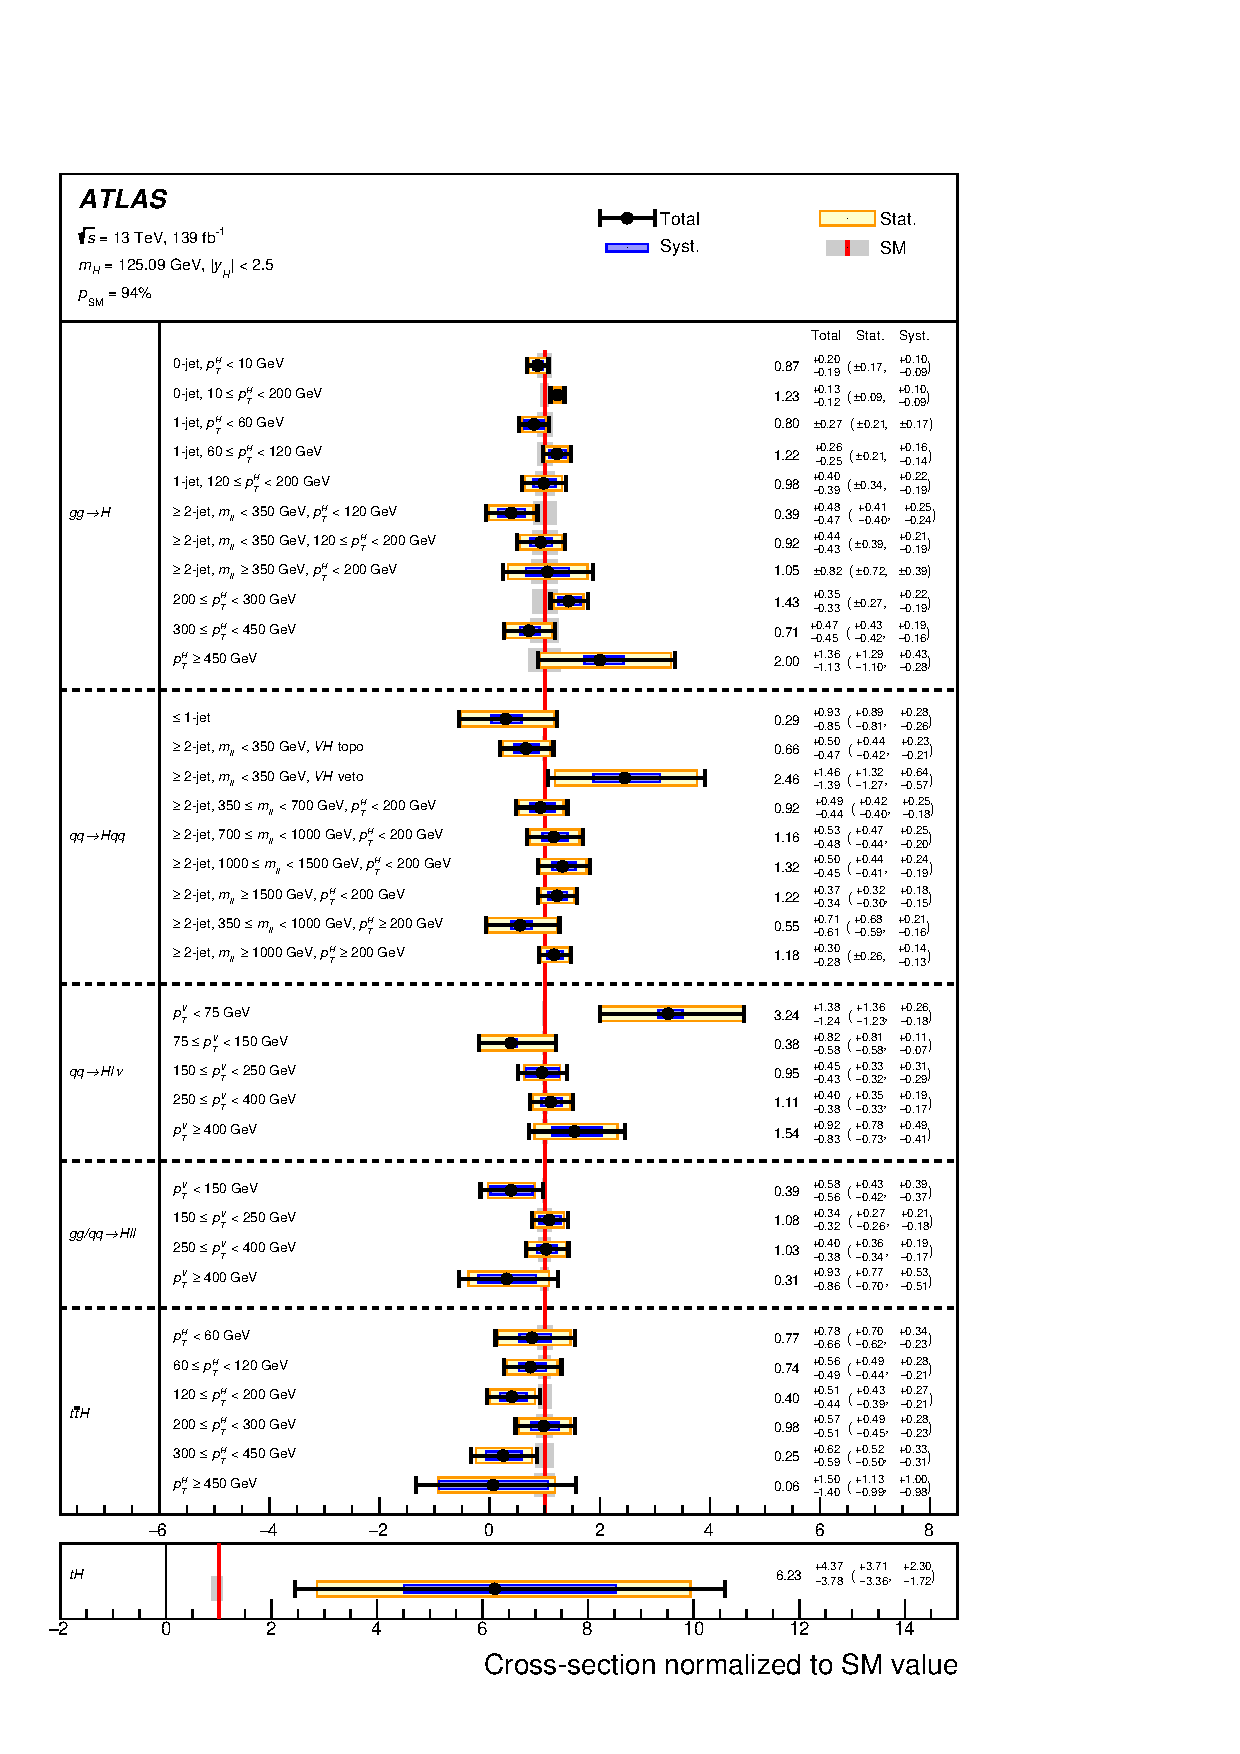
\includegraphics[width=0.75\textwidth]{atlas_stxs_results.pdf}
    \caption{Measurement of the Higgs boson production cross-section normalized to the SM predictions in 36 exclusive STXS regions using ATLAS Run-2 data. All these results are obtained assuming SM branching ratios for the Higgs boson decays. The error bars represent the total uncertainty in the measurement (in black), the statistical uncertainty (in yellow) and the systematic uncertainty (in blue)~\cite{Nature_ATLAS}.}
    \label{fig:atlas-stxs-results}
\end{figure}

This thesis contributes to extending the STXS measurements in the $H \to \tau \tau$ decay channel, with particular emphasis on the $t\bar{t}H$ production mode. The analysis strategy and detailed results are presented in Chapter~\ref{chap:htautau}. Note that the results shown in Figure~\ref{fig:atlas-stxs-results} do not yet include the $H \to \tau \tau$ channel measurements presented in this document.


%-------------------------------------------------------------------------------

%-------------------------------------------------------------------------------
\chapter{The LHC and the ATLAS Experiment}
\label{chap:ATLAS}
This chapter presents the experimental setup that has made possible the studies discussed throughout this thesis. It introduces the Large Hadron Collider (\acrshort{lhc}), a proton--proton collider located at the research complex of the Conseil Européen pour la Recherche Nucléaire (\acrshort{cern}). Subsequently, a description of the ATLAS (A Toroidal LHC ApparatuS) detector is provided, as it is the experiment from which the data used in this analysis have been collected.

%++++++++++++++++++++++++++++++++++++++++++++++
\section{The Large Hadron Collider}
\label{sec:LHC}
%++++++++++++++++++++++++++++++++++++++++++++++

The Large Hadron Collider (\acrshort{lhc}) is the world's largest and most powerful particle accelerator, situated at the \acrshort{cern} laboratory near Geneva, on the border between Switzerland and France. Founded in 1954, CERN is a European intergovernmental organization with the primary mission of advancing fundamental research in high-energy physics. It has become a global hub for scientific collaboration, involving over 20 member states and thousands of scientists and engineers from across the world.

The \acrshort{lhc} is the flagship project of \acrshort{cern}'s accelerator complex, and represents one of the most ambitious scientific endeavours in history. Its primary goals include performing precision measurements of \acrshort{sm} processes in order to be sensitive to any possible deviation, and searching for signs of new physics phenomena beyond the current theoretical framework, such as supersymmetry, extra dimensions, or dark matter candidates, as discussed in Section~\ref{sec:BSM}. The LHC's predecessor in the energy frontier was the Tevatron collider at Fermilab (USA), which operated at a centre-of-mass energy of 1.96~TeV. With its design energy of up to 14~TeV, the LHC has dramatically extended the discovery potential in the high-energy frontier, culminating in landmark achievements such as the discovery of the Higgs boson in 2012~\cite{ATLAS:2012yve,CMS:2012qbp}.

%xxxxxxxxxxxxxxxxxxxxxxxxxxxxxxxxxxxxxxxxxxxxxxxxxxxxxx
\subsection*{Overview and layout of the LHC}
%xxxxxxxxxxxxxxxxxxxxxxxxxxxxxxxxxxxxxxxxxxxxxxxxxxxxxx

The \acrshort{lhc} is a nearly circular accelerator with a circumference of 27~km, located about 100~m underground~\cite{Lyndon:Evans_2008}. It consists of two counter-rotating beam pipes, each containing a beam of protons (or heavy ions in some cases), which are accelerated to ultra-relativistic energies and made to collide at specific interaction points. These collision points are surrounded by four main detectors: \acrshort{atlas}, \acrshort{cms}, \acrshort{alice}, and \acrshort{lhcb}, each optimized for different types of physics analyses. While \acrshort{atlas}~\cite{ATLAS:exp} and \acrshort{cms}~\cite{CMS:exp} are general-purpose detectors designed to explore a broad range of physics topics, \acrshort{alice}~\cite{ALICE:exp} focuses on the beforehand mentioned heavy-ion collisions to study the quark–gluon plasma, and \acrshort{lhcb}~\cite{LHCb:exp} specializes in flavour physics and CP violation in the decays of heavy-flavour hadrons.

Protons are injected into the \acrshort{lhc} via a complex chain of smaller accelerators. Firstly, hydrogen atoms are ionized and resulting protons are accelerated up to 50~MeV by the linear accelerator, the LINAC2. They are then injected in the Proton Synchrotron Booster (PSB), which is followed by the Proton Synchrotron (PS) and the Super Proton Synchrotron (SPS), ending with the beams of protons reaching energies of 1.4~GeV, 26~GeV and 450~GeV, respectively. All these stages are represented in Figure~\ref{LHC:chain}. The PS and SPS pack protons to the LHC ring in bunches, which in nominal conditions are separated by 25 ns and a total of 2808 bunches can be finally delivered. Each of these bunches, containing around $10^{11}$ protons, are kept circulating inside the \acrshort{lhc} using superconducting magnets (mainly dipoles and quadrupoles) cooled to 1.9~K with liquid helium. Bending and focusing of the proton beams is needed since, as mentioned, the \acrshort{lhc} ring is not really circular, 
but composed of eight arcs and eight straight sections between them, 520 meters long each. This straight sections connects to the surface installations by lifts, where the main experiments mentioned above are located.

\begin{figure}[htbp]
    \centering
    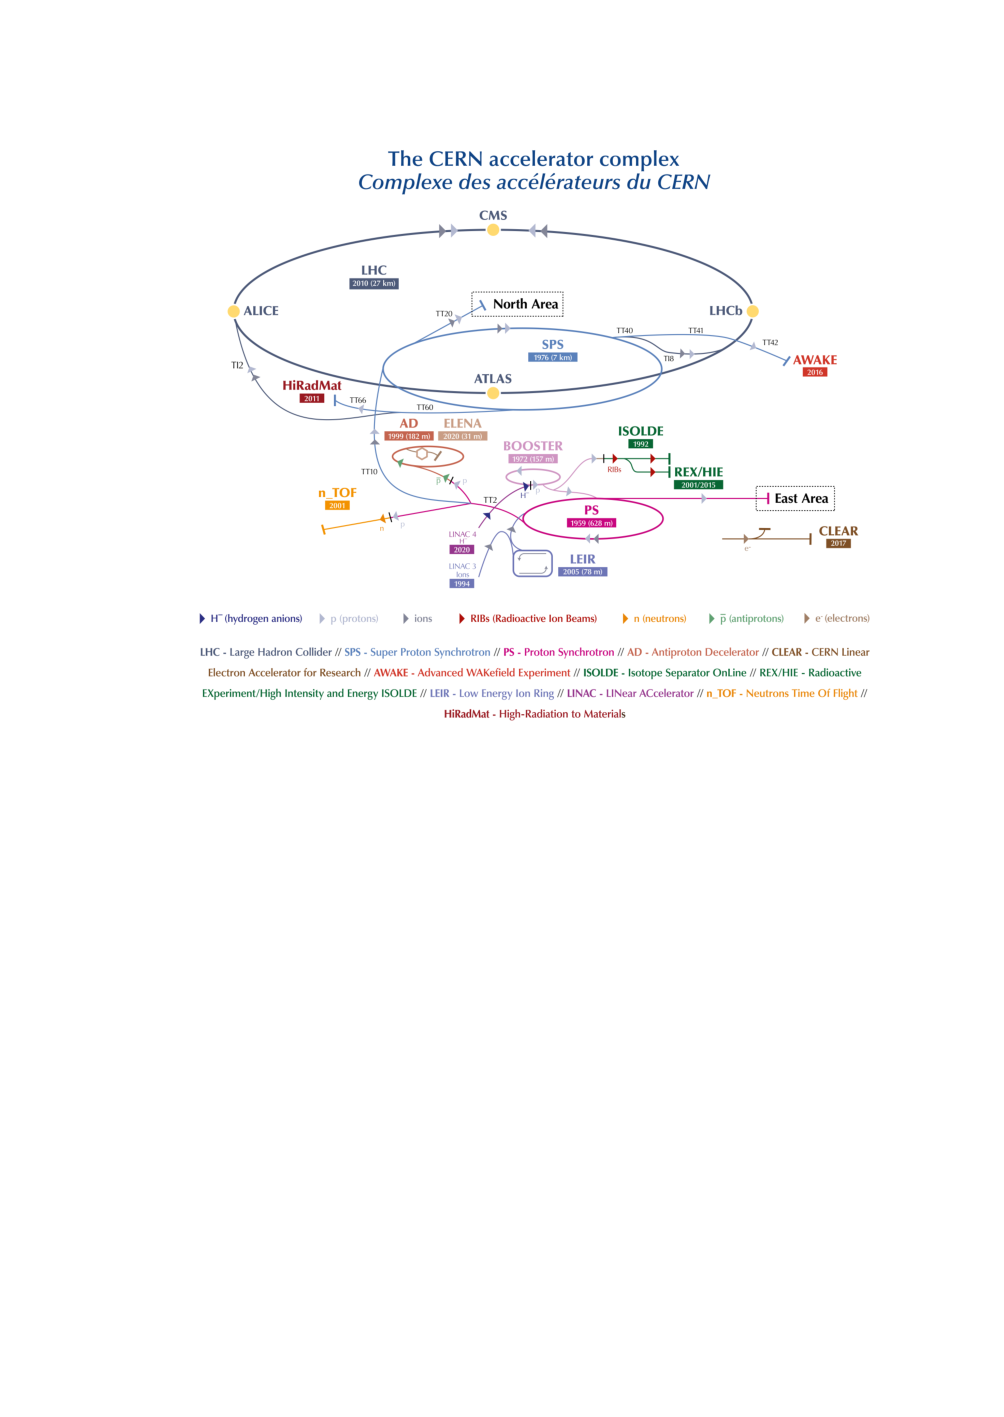
\includegraphics[width=1\linewidth]{images/CCC-v2022}\\
    \caption{Schematic overview of the CERN accelerator complex: the Large Hadron Collider, its injection chain and the four main experiments that record the collisions~\cite{Lopienska:2800984}}
    \label{LHC:chain}
\end{figure}


%xxxxxxxxxxxxxxxxxxxxxxxxxxxxxxxxxxxxxxxxxxxxxxxxxxxxxx
\subsection*{Beam conditions and luminosity}
%xxxxxxxxxxxxxxxxxxxxxxxxxxxxxxxxxxxxxxxxxxxxxxxxxxxxxx

Besides the energy that LHC can deliver to the colliding protons, another important performance characteristic of the accelerator is the number of events it is capable of producing. If one considers the instantaneous luminosity as a measure of the particle flux, then in a scattering process such as proton--proton collisions, the number of collisions can be expressed as:

\begin{equation}
  N_\text{{events}} = \sigma_{\text{event}} \int L\text{d}t = \sigma_{\text{event}}\mathcal{L},
\end{equation}
which is proportional to the cross-section representing the underlying physics of the process of interest, $\sigma_{\text{event}}$, such as Higgs boson production. The time integral over the instantaneous luminosity is referred to as the integrated luminosity, $\mathcal{L}$. The instantaneous luminosity depends on the properties of the beams and can be expressed as follows~\cite{Aad_2023}:
\begin{equation}
    L = f_{\text{rev}}\frac{N_1 N_2 N_b}{4\pi \sigma_x \sigma_y},
\end{equation}
where $N_b$ is the number of bunches per beam, $N_1$ and $N_2$ are the number of protons per bunch and $f_{\text{rev}}$ is the revolution frequency. In practice not all bunches are filled with electrons, and moreover these proton packs have extensions in both two directions perpendicular to the beam propagation direction assuming an effective gaussian shape with area $4\pi\sigma_{x}\sigma{y}$, being $\sigma_{x}$ and $\sigma_{y}$ the horizontal and vertical gaussian widths respectively.  

The integrated luminosity is typically expressed in units of inverse femtobarns (fb$^{-1}$), where $1~\text{fb}^{-1} = 10^{39}~\text{cm}^{-2}$. Figure~\ref{figure:Run3lumi}(a) shows the integrated luminosity delivered to ATLAS for each year of data taking from 2011 to 2025. Figure~\ref{figure:Run3lumi}(b) displays a comparison between the cumulative luminosity delivered and recorded by the ATLAS detector during Run~2, the data-taking period from 2015 to 2018, which constitutes the main dataset analysed in this thesis, along with the early years of Run~3.

\acrshort{atlas} collected approximately 147~fb$^{-1}$ of proton--proton collision data at a center-of-mass energy of 13~TeV during Run~2. However, not all delivered data are suitable for physics analysis. The dataset certified for physics-quality analyses, i.e.\ the one included in the Good Run List (GRL)~\cite{Aad_2020}, is slightly smaller due to quality and detector performance criteria. Specifically, ATLAS recorded a total of $140 \pm 1.2$~fb$^{-1}$ of high-quality data during Run~2, and approximately 166~fb$^{-1}$ during the years 2022--2024 of Run~3.

\begin{figure}[htbp]
\centering
\begin{tabular}{cc}
    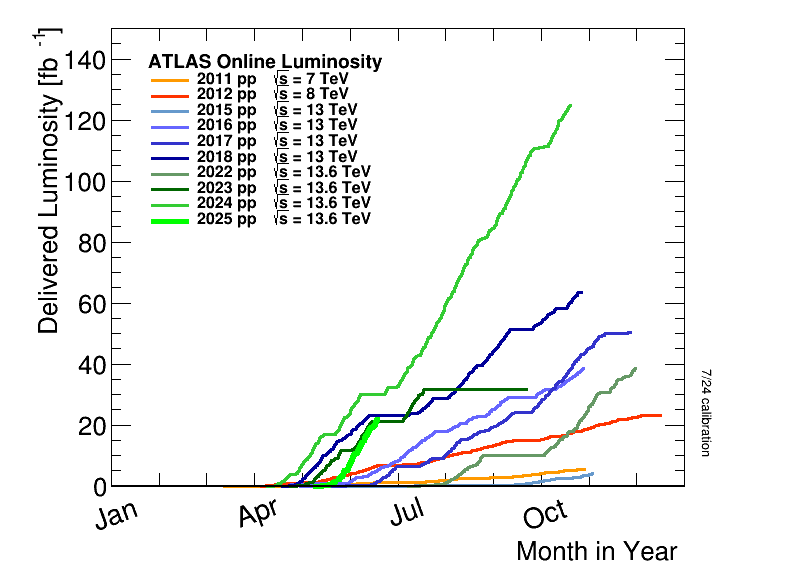
\includegraphics[width=0.5\linewidth]{images/intlumivsyear.png} &
    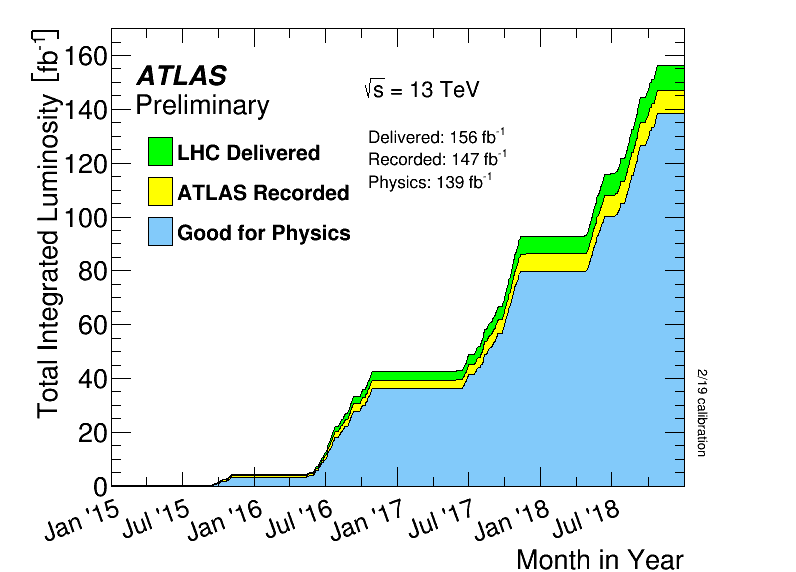
\includegraphics[width=0.5\linewidth]{images/intlumivstimeRun2DQall.png} \\
    (a) & (b)  \\
\end{tabular}
\caption{(a) Cumulative pp collision luminosity delivered to the ATLAS detector versus month
of the year, separately for years between 2011 and 2024~\cite{atlas:Run3lumi} and (b) cumulative luminosity versus
time delivered by the LHC (green), recorded by ATLAS (yellow) and used for physics (blue)
during stable beams for pp collisions at 13 TeV centre-of-mass energy in years 2015-2018~\cite{atlas:Run2lumi}}
\label{figure:Run3lumi}
\end{figure}

%xxxxxxxxxxxxxxxxxxxxxxxxxxxxxxxxxxxxxxxxxxxxxxxxxxxxxx
\subsection*{Pile-up and its challenges}
%xxxxxxxxxxxxxxxxxxxxxxxxxxxxxxxxxxxxxxxxxxxxxxxxxxxxxx

As previously mentioned, the proton bunches that collide at the various interaction points (IPs) of the \acrshort{lhc} contain a large number of protons. As a consequence, it is common for more than one hard proton--proton scattering to occur in a single bunch crossing. This phenomenon is known as pile-up.

More precisely, we refer to the average number of proton--proton interactions per bunch crossing to quantify this effect, since the number of interactions can vary depending on the beam conditions. Pile-up can be classified into two categories: in-time pile-up, which refers to multiple interactions occurring within the same bunch crossing, and out-of-time pile-up, which originates from proton--proton interactions taking place in neighboring bunch crossings. The latter can affect the measurements when the readout times of the detector systems exceed the time interval between consecutive bunches, complicating the identification of the primary vertex and the correct association of final-state particles to it.

The number of interactions per bunch crossing follows a Poisson distribution, with a mean value $\mu$ proportional to the product of the total inelastic proton--proton cross-section $\sigma_{\text{inel}}$ and the instantaneous luminosity~\cite{pileup}
\begin{equation}
    \mu = \frac{\text{L}_{\text{bunch}}\sigma_{\text{inel}}}{f_{\text{rev}}}.
\end{equation}
Figure~\ref{fig:pileup} shows the distribution of this mean number of interactions per bunch crossing during both Run 2 and Run 3 data-taking periods of \acrshort{atlas}.
Increasingly efforts are being devoted to develop mitigation strategies for this effect, especially thinking about future scenarios as the HL-LHC, including advanced pile-up suppression techniques, such as vertex association, pile-up subtraction in jets and missing energy, and the use of machine learning algorithms to distinguish primary vertices from pile-up vertices~\cite{ATL-PHYS-PUB-2023-011,ATLAS:2017pfq,Soyez_2019}.
\begin{figure}[htbp]
    \centering
    \begin{tabular}{cc}
        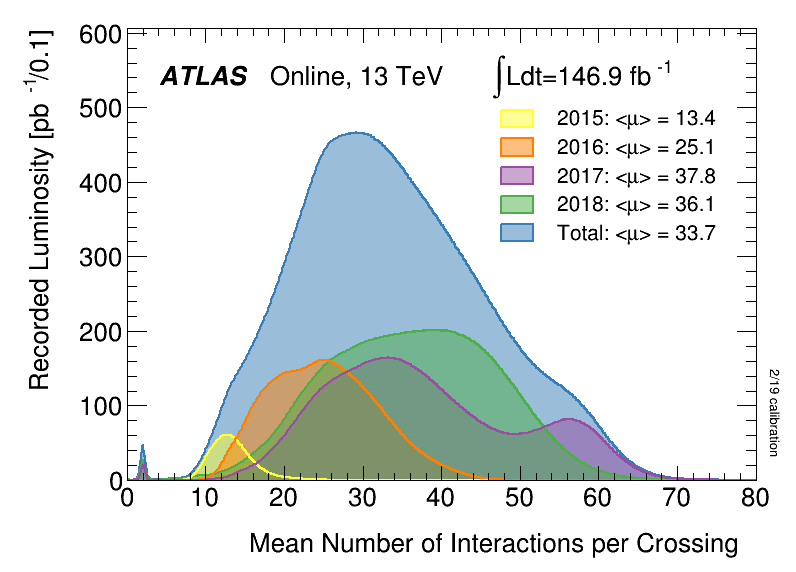
\includegraphics[width=0.5\linewidth]{images/mu_2015_2018.png} &
        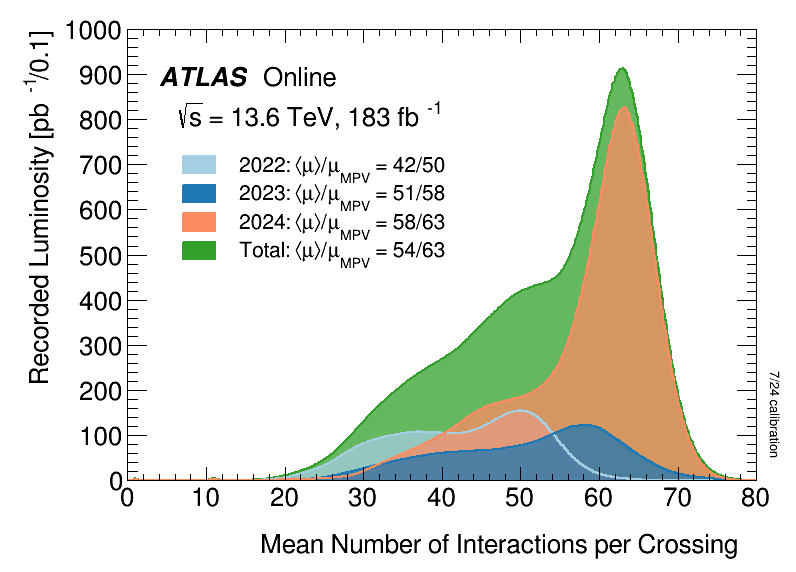
\includegraphics[width=0.5\linewidth]{images/mu_2022_2024.png} \\
        (a) & (b)  \\
    \end{tabular}
    \caption{(a) Distribution of mean number of interactions per bunch crossing in data recorded by the \acrshort{atlas} experiment at 13~TeV during Run 2~\cite{atlas:Run2lumi} and  (b) at 13.6~TeV during Run 3~\cite{atlas:Run2lumi} data-taking periods.}
    \label{fig:pileup}
    \end{figure}
%xxxxxxxxxxxxxxxxxxxxxxxxxxxxxxxxxxxxxxxxxxxxxxxxxxxxxx
\subsection*{LHC upgrade plans}
%xxxxxxxxxxxxxxxxxxxxxxxxxxxxxxxxxxxxxxxxxxxxxxxxxxxxxx

To further push the frontiers of high-energy physics and enhance the physics reach of the LHC programme, a major upgrade of the collider and its experiments is underway. The High-Luminosity LHC (HL-LHC) project~\cite{HLLHC} aims to increase the integrated luminosity delivered to the experiments by more than an order of magnitude, targeting up to 3000~fb$^{-1}$ of proton--proton collision data by the end of the next decade.

This increase in data volume will significantly improve the statistical precision of measurements of rare processes and enable detailed studies of the Higgs boson properties, electroweak interactions, and potential signals of physics beyond the Standard Model. In particular, the HL-LHC will allow for precise measurements of Higgs boson couplings, self-interactions, and rare decays, as well as the potential observation of extremely suppressed processes such as flavour-violating decays or double Higgs production.

Achieving the HL-LHC goals requires a broad range of upgrades to the accelerator complex and its associated infrastructure. Key improvements include the installation of new high-field superconducting quadrupole magnets near the interaction points, based on advanced Nb$_3$Sn technology~\cite{Mangiarotti:2770766}, which will allow for a reduction in the beams width, and consequently, an increase in luminosity. Additionally, new cryogenic and collimation systems will be implemented to handle the increased beam power and radiation levels.

On the experiment side, all main LHC experiments, including ATLAS, are undergoing substantial upgrades to handle the harsher conditions of HL-LHC operation. These include the development of new inner trackers with extended radiation hardness and granularity, the replacement of calorimeter and muon chamber readout electronics to support higher data rates, and a completely redesigned trigger and data acquisition system. The upgraded detectors must be capable of maintaining excellent performance in the presence of average pile-up levels exceeding $\langle\mu\rangle \sim 140$, more than a factor of two higher than those typically encountered during Run~3.

The HL-LHC project is expected to start operations by 2029, following the completion of the Long Shutdown 3 (LS3). It represents the next major milestone in the LHC physics programme, with the potential to open a new era of precision measurements and exploration of the unknown.


%++++++++++++++++++++++++++++++++++++++++++++++
\section{The ATLAS detector}
\label{sec:ATLAS}
%++++++++++++++++++++++++++++++++++++++++++++++

Having already outlined the design, physics programme and scientific goals of the LHC experiment, this section presents in detail each of the main components that make up the ATLAS detector.

ATLAS (A Toroidal LHC ApparatuS)~\cite{ATLAS:exp,ATLAS:1999uwa} is a general-purpose detector designed to explore a wide spectrum of physics phenomena, ranging from precision tests of the Standard Model to searches for new particles and interactions beyond it. It is the largest 
detector ever constructed for a collider experiment, with a cylindrical geometry approximately 44~m long, 25~m diameter, and weighing over 7000~tons. Its conception, design and construction were carried out by a global collaboration of more than 3000 scientists and engineers from around 180 institutions in nearly 40 countries.

Data-taking with ATLAS began in 2009, when the LHC first delivered proton-proton collisions. Since then, the detector has been instrumental in several landmark achievements, most notably the discovery of the Higgs boson in 2012. The ATLAS detector is composed of multiple subdetectors arranged in concentric layers 
around the interaction point. The cylindrical structure is closed by two end-caps, providing almost $4\pi$ coverage of the solid angle. An illustration of the ATLAS detector can be found in Figure~\ref{fig:ATLASdet}.

The different ATLAS subsystems are designed to measure the properties of different types of particles. In the innermost region, closest to the interaction point, the inner detector is built to record the properties of charged particles produced in the collisions. Their trajectories 
are bent by a 2~T magnetic fields produced by a superconducting solenoid. Then, the inner detector is surrounded by the calorimeter system which is in charge of measuring the energy of particles that can produce electromagnetic and hadronic showers in the detector. It is striped in a liquid argon electromagnetic calorimeter and a hadronic calorimeter composed by a scintillating barrel and liquid argon end-caps.
In the outermost region of the detector it is placed the muon spectrometer, devoted to the measurement of muons produced in the collision and which are bent by a 4~T magnetic field produced in this case by a toroidal magnet system.
The following sections describe the purpose and operating principles of these components in detail, as well as the forward detectors and the trigger and data acquisition system.

\begin{figure}[htbp]
    \centering
        \includegraphics[width=1\linewidth]{ATLAS-Experiment-Schematic-2022-Labels-People.png}
    \caption{Cut-away view of the Run~3 configuration of the \acrshort{ATLAS} detector indicating the locations of the larger detector sub-systems~\cite{Bianchi:2837191}.}
    \label{fig:ATLASdet}
\end{figure}

%xxxxxxxxxxxxxxxxxxxxxxxxxxxxxxxxxxxxxxxxxxxxxxxxxxxxxx
\subsection{Reference frames and coordinate system}
\label{sec:coordinates}
%xxxxxxxxxxxxxxxxxxxxxxxxxxxxxxxxxxxxxxxxxxxxxxxxxxxxxx

The ATLAS experiment adopts a right-handed coordinate system, centered at the nominal interaction point (IP) where the proton--proton collisions take place. The origin of the coordinate system lies at the geometrical center of the detector. The $z$-axis is defined along the beam pipe, pointing in the direction of the anti-clockwise beam. The $x$-axis points from the IP towards the center of the LHC ring, while the $y$-axis points upwards, 
completing a right-handed coordinate system. The transverse plane defined by $x$ and $y$ directions locate important observables like the transverse momentum ($p_{T}$) and the so-called missing transverse momentum ($E^{miss}_{T}$).

In addition to the Cartesian coordinates $(x, y, z)$, a cylindrical coordinate system is often used due to the symmetry of the detector. In this system, the transverse plane is defined by the coordinates $(r, \phi)$, where $r$ is the radial distance from the $z$-axis and $\phi$ is the azimuthal angle measured around the beam pipe. The longitudinal direction remains aligned with the $z$-axis.

To describe the polar angle of a particle’s trajectory, defining deviations from the beam direction, the rapidity $y$ is preferred over the polar angle $\theta$, as it is invariant under Lorentz boosts along the $z$-axis:
\begin{equation}
    y = \frac{1}{2}\ln{\frac{E+p_{Z}}{E-{p_{Z}}}},
\end{equation}
where E is the particle's energy and $p_{Z}$ the longitudinal component of its momentum. In the ultra-relativistic limit, this variable can be approximated by the so-called pseudorapidity, $\eta$, since the mass of most of final-state particles is mostly negligible against their momenta:
\begin{equation}
\eta = -\ln \tan \left( \frac{\theta}{2} \right).
\end{equation}
In this frame, if a particle is emmitted in the beam direction, $\theta \rightarrow 0º$, it would have assigned $\eta \rightarrow \infty$, while if it follows a direction perpendicular to the beam, $\theta = 90º$ corresponds to $\eta = 0$.
The angular distance between two objects in the detector is typically measured using the $\Delta R$ metric in the $(\eta, \phi)$ plane:
\begin{equation}
\Delta R = \sqrt{(\Delta \eta)^2 + (\Delta \phi)^2}.
\end{equation}

This coordinate convention is used throughout the analysis and the design of the detector subcomponents, as well as in reconstruction and identification algorithms for physics objects such as jets, leptons, and missing transverse energy. It is illustrated in Figure~\ref{fig:coord}.
\begin{figure}[htbp]
    \centering
        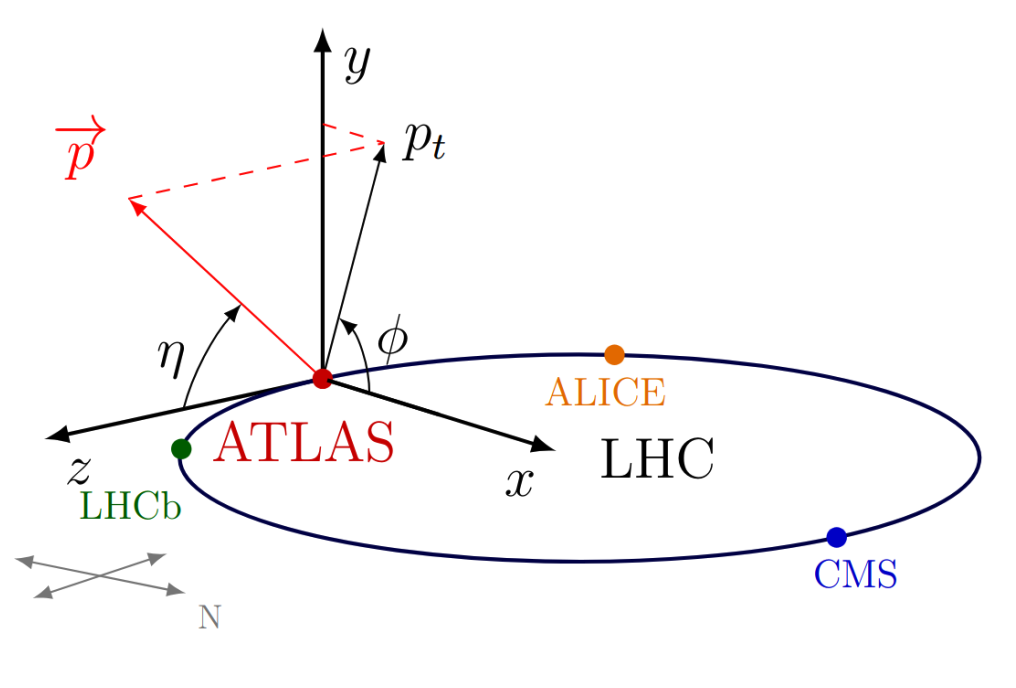
\includegraphics[width=0.7\linewidth]{ATLAS_coordinates.png}
    \caption{Illustration of the ATLAS coordinate system. Image obtained from Ref.~\cite{coordinates}.}
    \label{fig:coord}
\end{figure}

%xxxxxxxxxxxxxxxxxxxxxxxxxxxxxxxxxxxxxxxxxxxxxxxxxxxxxx
\subsection{Inner detector}
\label{sec:ID}
%xxxxxxxxxxxxxxxxxxxxxxxxxxxxxxxxxxxxxxxxxxxxxxxxxxxxxx


The Inner Detector (ID)~\cite{id1,id2} is the central tracking system of the ATLAS experiment and plays a fundamental role in the reconstruction of charged particles emerging from proton-proton collisions. It is the innermost component of the detector, positioned directly around the interaction point, and it is enclosed within a thin superconducting solenoid that generates a 2~T magnetic field parallel to the beam axis. This magnetic field bends the trajectory of charged particles in the $\phi$ direction, which allows the determination of their charge and momentum due to this curvature.

The ID is composed of three complementary subdetectors arranged in layers from the innermost to the outermost radii: the Pixel Detector, the Semiconductor Tracker (SCT), and the Transition Radiation Tracker (TRT). The Pixel and SCT systems are based on silicon technologies and are optimized for high spatial resolution and precision tracking, particularly near the primary vertex, which is the measured spatial location where the hard scattering of partons of interest in a given event took place. In contrast, the TRT is a gaseous detector made of straw tubes and is designed to extend the tracking capabilities at higher radii while also enhancing electron identification through the detection of transition radiation.

Together, these three subdetectors span a cylindrical volume of approximately 6.2~m in length and 2.1~m in diameter, and provide tracking coverage in the pseudorapidity range of $|\eta| < 2.5$. The layout of the ID is divided into a central barrel region ($|\eta| < 1.4$) and two symmetric endcap sections ($1.4 < |\eta| < 2.5$). As charged particles traverse the ID, they produce hits in the different layers, which are then used to reconstruct their trajectories with high efficiency and resolution. This track information is vital for identifying not only primary vertices, but other vertices that are displaced from the primary one and could originate from the decay of heavy-flavour hadrons that travels enough before decaying. This is clearly essential for tagging of these jets, and supporting particle identification algorithms throughout the ATLAS reconstruction chain, as will be explained in Chapter~\ref{chap:object_rec}.
An schematic view of the barrel section of the ID can be found in Figure~\ref{fig:id}.
\begin{figure}[htbp]
    \centering
        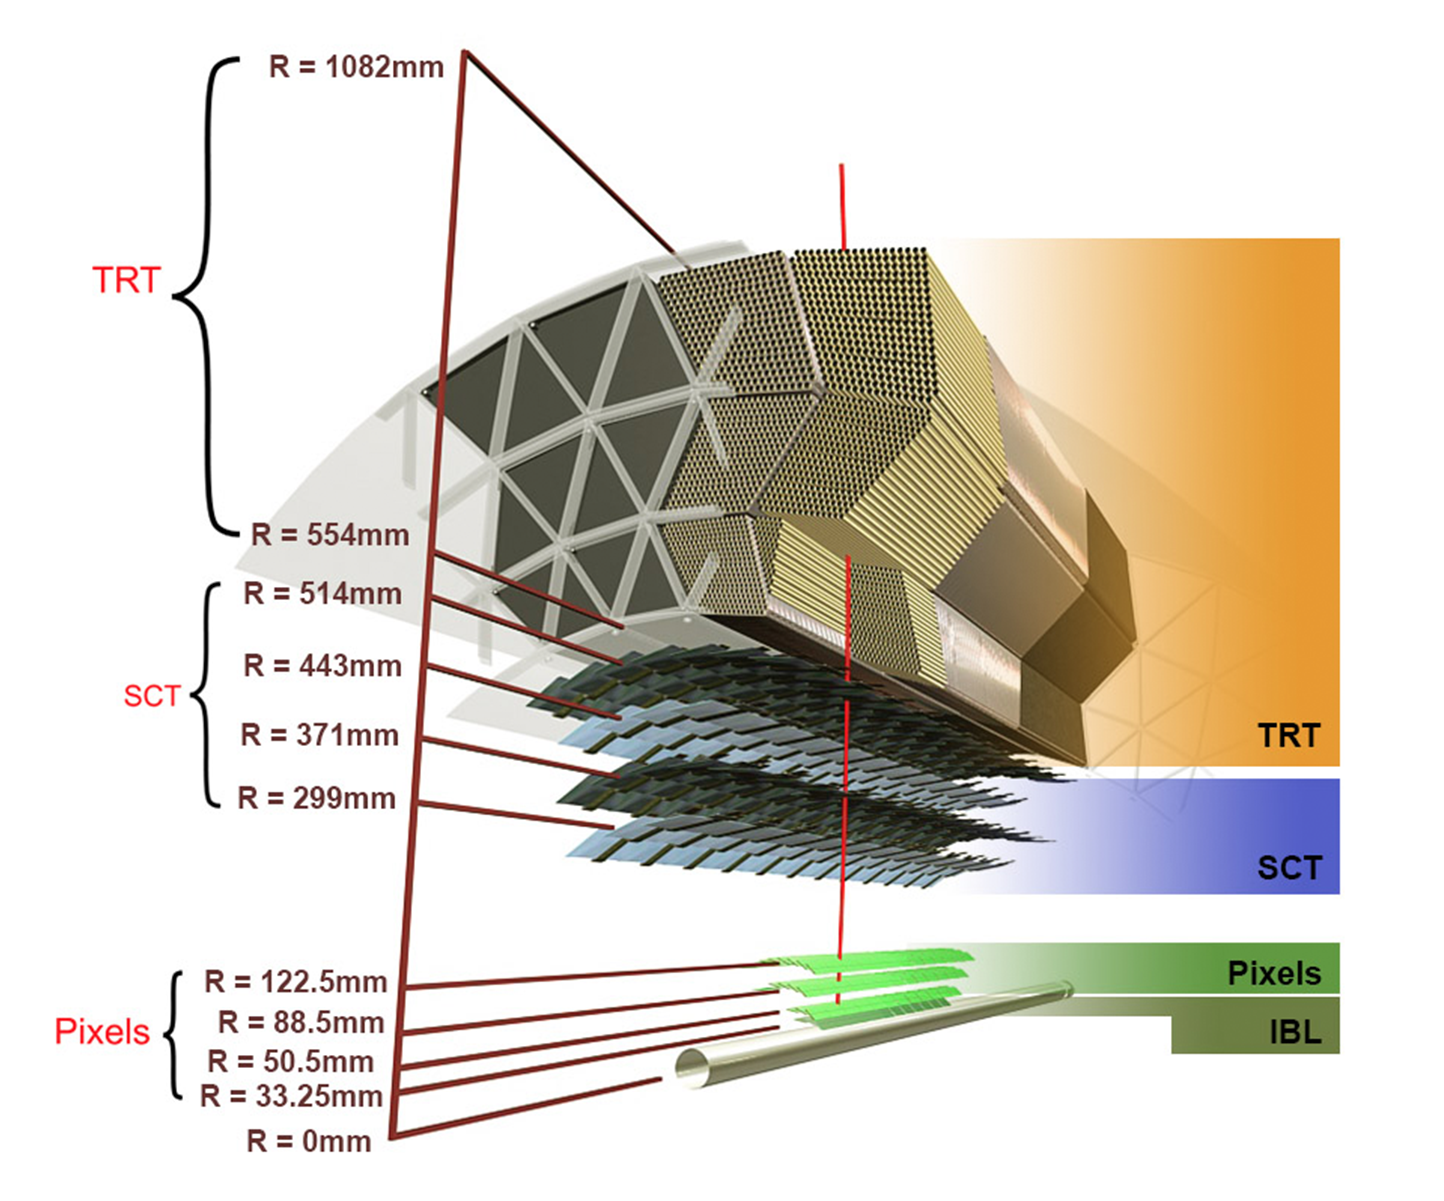
\includegraphics[width=0.7\linewidth]{ATLAS_id.png}
    \caption{Cutaway representation of the barrel section of the ATLAS inner detector. From the innermost to the outermost layers, it shows the pixel detector, the four cylindrical an concentrical layer of the SCR and the straw tubes characteristic of the TRT~\cite{Collaboration:2723878}.}
    \label{fig:id}
\end{figure}

\subsubsection*{Pixel detector}

The Pixel Detector is the innermost and most granular component of the ID. Its layout consists of three cylindrical layers of silicon pixel sensors in the barrel region, positioned at radial distances of 50.5, 88.5, and 122.5~mm, and three disks per endcap located at $z = \pm$495, 580, and 650~mm. The sensors in these layers have pixel sizes of $50 \times 400~\mu\text{m}^2$ and a thickness of 250~$\mu$m. This geometry yields a spatial resolution of about $10~\mu$m in the $r\text{--}\phi$ plane and $115~\mu$m in $z$ for the barrel region, and the opposite in the endcaps, where resolution is optimized along $z$.

In preparation for Run~2, an additional innermost layer known as the Insertable B-Layer (IBL)~\cite{IBL} was installed at a radius of 33.25~mm. The IBL significantly improved the impact parameter resolution, particularly for low-$p_{\mathrm{T}}$ tracks. It is composed of both planar and 3D silicon sensors with reduced pixel dimensions of $50 \times 250~\mu\text{m}^2$ and sensor thicknesses of 250~$\mu$m and 200~$\mu$m, respectively. The closer proximity of the IBL to the beamline and its finer segmentation improves its ability to separate primary and secondary vertices even under high occupancy conditions, which is crucial for the identification of jets originating from heavy-flavour quarks.

During Run~3, the Pixel Detector has been operating under increasingly harsh radiation environments and elevated levels of pile-up. These conditions challenge the performance and life-time of the system, especially the innermost layers. Dedicated calibration and alignment strategies, as well as enhanced readout electronics, are employed to preserve the resolution and efficiency of tracking throughout this demanding phase of operation.

\subsubsection*{Semiconductor Tracker (SCT)}

Outwards, the SCT subdetector follows the pixel one, consisting of four barrel layers and nine disks in each endcap, built with silicon microstrip modules. Each module includes two sensors, mounted back-to-back at a small stereo angle of 40 mrad, enabling precise 3D position reconstruction of $17$~$\mu$m resolution in the transverse plane and $580$~$\mu$m in the longitudinal direction. 
The SCT contains around 6 million readout channels.

\subsubsection*{Transition Radiation Tracker (TRT)}

The TRT is the outermost component of the Inner Detector and extends tracking capabilities up to $|\eta| < 2.0$, complementing the precise position measurements from the inner silicon detectors with additional points along the track path. The TRT also provides particle identification (PID) capabilities, particularly useful for electron-pion discrimination via detection of transition radiation photons.

It consists of a large number of thin straw tubes, 52,544 in the barrel region and 122,880 in the two endcaps, each with a diameter of 4~mm. These tubes are originally filled with a gas mixture of 70\% xenon, 27\% carbon dioxide, and 3\% oxygen. When a charged particle traverses a straw, it ionizes the gas along its path. A high negative voltage applied to the tube walls causes the liberated electrons to drift toward a central anode wire, producing a detectable signal. 

The TRT delivers a spatial resolution of approximately $130~\mu\text{m}$ in the $r\text{--}\phi$ plane and contributes on average about 30 measurement points per track, thus enhancing the momentum resolution and the track reconstruction efficiency, especially for high-$|\eta|$ regions where fewer silicon hits are available. Its ability to identify transition radiation, photons emitted by relativistic electrons crossing dielectric boundaries embedded in the tracker, provides an additional layer of particle identification crucial for several physics analyses.

During Run~3, it has been used an argon-based gas mixture in the entire barrel and part of the end-cap region to minimize xenon loss and ensure gas stability. Although this reduces the barrel's PID performance due to weaker transition radiation photon absorption, it still provides useful electron identification when combined with d$E$/d$x$ information. The end-cap PID performance remains largely preserved~\cite{ATLAS_run3}.

\vspace{-0.3}
At this stage it is worth noting that, ahead of Run 3, an important part of the read-out electronics in several sub-detectors were refurbished and optimised to withstand the higher data rates expected during this period. By the end of Run~3 the existing silicon trackers will be operating close to their radiation-tolerance limits, and the TRT will no longer be able to function under the nominal HL-LHC conditions. To preserve vertex-tagging and track-reconstruction performance, the entire Inner Detector will therefore be superseded by an all-silicon Inner Tracker (ITk). In addition, a High-Granularity Timing Detector will be installed in the forward region in order to match tracks with calorimeter clusters using precise time information, that is an essential tool for mitigating the extreme pile-up foreseen at the HL-LHC \cite{ATLAS:1502664}
%xxxxxxxxxxxxxxxxxxxxxxxxxxxxxxxxxxxxxxxxxxxxxxxxxxxxxx
\subsection{Calorimeters}
\label{sec:calo}
%xxxxxxxxxxxxxxxxxxxxxxxxxxxxxxxxxxxxxxxxxxxxxxxxxxxxxx
Moving outwards again, beyond the solenoid magnet containing the Inner Detector, we find the ATLAS calorimeter system~\cite{lar_tech,tile_tech}, which fully encloses the previously described 
components. Both types of calorimeters, electromagnetic and hadronic, cover a total range up to $|\eta| < 4.9$, allowing for the measurement of the energy of particles traversing them, 
as they are nominally designed to completely absorb the energy of most particles predicted by the \acrshort{sm}, 
except for muons and neutrinos. An schematic illustration of the ATLAS calorimeter system is shown in Figure~\ref{fig:cal}.
\begin{figure}[htbp]
    \centering
        \includegraphics[width=0.9\linewidth]{ATLAS_cal.jpg}
    \caption{Cutaway representation of the ATLAS calorimeter system and its main components~\cite{Collaboration:2723878}.}
    \label{fig:cal}
\end{figure}

%%%%%%%%%%%%%%%%%%%%%%%%%%%%%%%
\subsubsection{LAr electromagnetic calorimeter}
\label{sec:elelar}
%%%%%%%%%%%%%%%%%%%%%%%%%%%%%%%

The electromagnetic calorimeter (EM calorimeter) in the ATLAS detector is designed to precisely measure the energy of electrons and photons. It is based on a sampling technology that uses liquid argon (LAr) as the active medium and different metals (either tungsten, copper or lead) as the absorber material. This choice combines a high level of granularity with excellent linearity and radiation hardness, crucial for operation in the high-luminosity environment of the LHC.

The EM calorimeter is divided into three main regions: a barrel section covering the pseudorapidity range $|\eta| < 1.475$ (EMB), and two end-cap sections (EMEC) that extend the coverage up to $|\eta| = 3.2$. Each region is segmented longitudinally into three layers (plus a presampler), as can be seen in Figure~\ref{fig:LAr_EM}, optimizing the reconstruction of electromagnetic showers. The presampler layer is used to correct for energy loss in the material upstream of the calorimeter. The first layer features fine granularity in the $\eta$ direction ($\Delta\eta = 0.0031$), allowing for precise discrimination between single photons and the two close-by photons resulting from $\pi^0$ decays. The second layer collects most of the energy from electromagnetic showers and provides the primary energy measurement. The third layer corrects for energy leakage at high energies.

\begin{figure}[htbp]
    \centering
        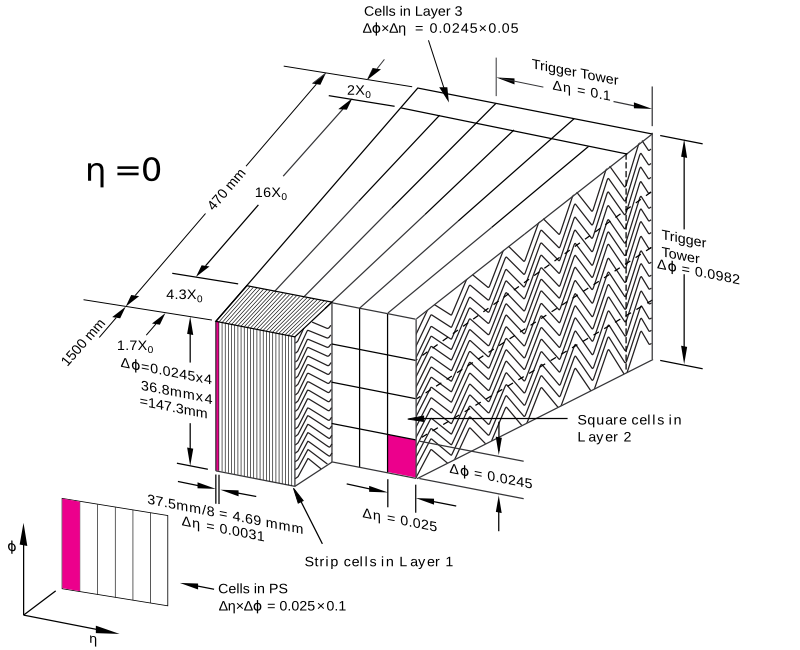
\includegraphics[width=0.8\linewidth]{LAr_EM.png}
    \caption{Schematic diagram of the cross-section of the LAr EM barrel calorimeter, including the presampler. The different granularity in $\eta$ and $\phi$ of the cells of each of the three layers is also shown~\cite{atlas:EM_LAr}}
    \label{fig:LAr_EM}
\end{figure}

The LAr calorimeter employs an accordion-shaped geometry in both the barrel and end-cap regions. This design ensures full azimuthal coverage without projective cracks, while maintaining uniform response and mechanical stability. The calorimeter modules are housed in cryostats filled with liquid argon, operating at a temperature of approximately 87~K. The readout cells are segmented into towers of size $\Delta\eta \times \Delta\phi = 0.025 \times 0.025$ in the second layer, which defines the granularity for standard electromagnetic object reconstruction.

The signal is induced by the ionization of the LAr by charged particles in the shower. Ionization electrons drift under a high-voltage electric field, and the resulting current is read out with high precision using fast, low-noise electronics, used to determine the energy deposited by the original particle that hit the detector. The typical energy resolution of the EM calorimeter is described by the expression:
\begin{equation}
\frac{\sigma_E}{E} = \frac{a}{\sqrt{E}} \oplus b \oplus \frac{c}{E},
\end{equation}
where $a$ represents the stochastic term (about $10\%$), $b$ the constant term (below $0.7\%$), and $c$ the noise term. The excellent resolution is essential for precision measurements such as the $H \rightarrow \gamma\gamma$ and $H \rightarrow ZZ^* \rightarrow 4\ell$ channels.

%%%%%%%%%%%%%%%%%%%%%%%%%%%%%%%
\subsubsection{LAr hadronic calorimeters}
\label{sec:elehad}
%%%%%%%%%%%%%%%%%%%%%%%%%%%%%%%

The hadronic calorimeter system complements the electromagnetic calorimeter by measuring the energy of hadrons. In the end-cap and forward regions, the hadronic calorimetry is provided by these LAr-based detectors: the Hadronic End-Cap Calorimeter (HEC) and the Forward Calorimeter (FCal). These systems are critical for reconstructing jets, missing transverse energy, and for identifying hadronically decaying $\tau$-leptons in the forward regions.

The HEC is positioned directly behind the EMEC and covers the pseudorapidity range $1.5 < |\eta| < 3.2$. It consists of copper plates as absorbers and uses liquid argon as the active medium. The copper-LAr combination ensures a compact structure with good radiation hardness and linearity. The HEC is segmented longitudinally into four layers and provides a depth of about 10 interaction lengths ($\lambda_0$) when combined with the electromagnetic calorimeter, enabling efficient hadronic shower containment. Each end-cap consists of two wheels: a front wheel (HEC1) constituted of 24 copper plates, and a rear wheel (HEC2) made of 16 copper plates.

The Forward Calorimeter (FCal) extends the coverage to $|\eta| < 4.9$ and is composed of three longitudinal modules: the first is electromagnetic, featuring copper absorbers, and the second and third are hadronic, and uses tungsten absorbers in order to reduce the lateral spread of the hadronic showers. The high-density design of the FCal is necessary to withstand the high particle flux and radiation levels encountered in the forward region. Due to its crucial role in reconstructing the forward energy flow, the FCal is also essential for pile-up suppression and missing transverse energy reconstruction.

Both HEC and FCal calorimeters operate within the same LAr cryostats as the electromagnetic sections, benefitting from the same stability and fast response. 

%%%%%%%%%%%%%%%%%%%%%%%%%%%%%%%
\subsubsection{Tile hadronic calorimeter}
\label{sec:tilecal}
%%%%%%%%%%%%%%%%%%%%%%%%%%%%%%%

The Tile Calorimeter (TileCal) is ATLAS's main hadronic calorimeter, constructed as a sampling calorimeter composed of alternating layers of plastic scintillator tiles (active material) and low-carbon steel absorber plates. Positioned around the LAr calorimeter, TileCal provides coverage in the pseudorapidity region $|\eta|<1.7$ and ensures containment of hadronic showers, limiting punch-through to the muon system with a total thickness of approximately 11~$\lambda_0$ at $\eta=0$.

TileCal consists of a central long barrel (LB) section ($|\eta|<1.0$, length of 5.8 m) and two extended barrel (EB) sections (EBA and EBC), each covering $0.8<|\eta|<1.7$ with a length of 2.6 m. Together with other calorimeters (HEC, FCal), TileCal achieves coverage up to $|\eta|<4.9$.

Each barrel segment is divided into 64 modules, featuring alternating 3 mm thick scintillator tiles and 14 mm thick steel absorbers along the beam axis. The scintillator tiles, arranged radially in 11 rows, generate scintillation light upon particle interaction. Wavelength-shifting (WLS) fibers collect and shift this light to longer wavelengths, guiding it to photomultiplier tubes (PMTs) at the module's outer radius, enabling efficient and hermetic readout.

The calorimeter modules are segmented into three longitudinal layers: layers A, BC, and D in the LB (1.5, 4.1, and 1.8 $\lambda_0$, respectively) and layers A, B, and D in the EB (1.5, 2.6, and 3.3 $\lambda_0$, respectively). Cells in these layers have granularity of $\Delta\eta \times \Delta\phi=0.1\times0.1$ for inner layers and $0.2\times0.1$ for outer layers.

Additionally, gap scintillator cells (E1-E4) were installed between TileCal and LAr to correct for energy losses and enhance performance. The Minimum-Bias Trigger Scintillators (MBTs), also read out by TileCal electronics, provide coverage in $2.08<|\eta|<3.86$ for triggering purposes. Overall, TileCal incorporates 9852 readout channels, covering 5182 cells.

Figure~\ref{fig:cal_resum} shows an schematic view of the readout geometry of all the calorimeter systems in the $r$--$z$ space, showing the different $\eta$ ranges covered by them.
\begin{figure}[htbp]
    \centering
        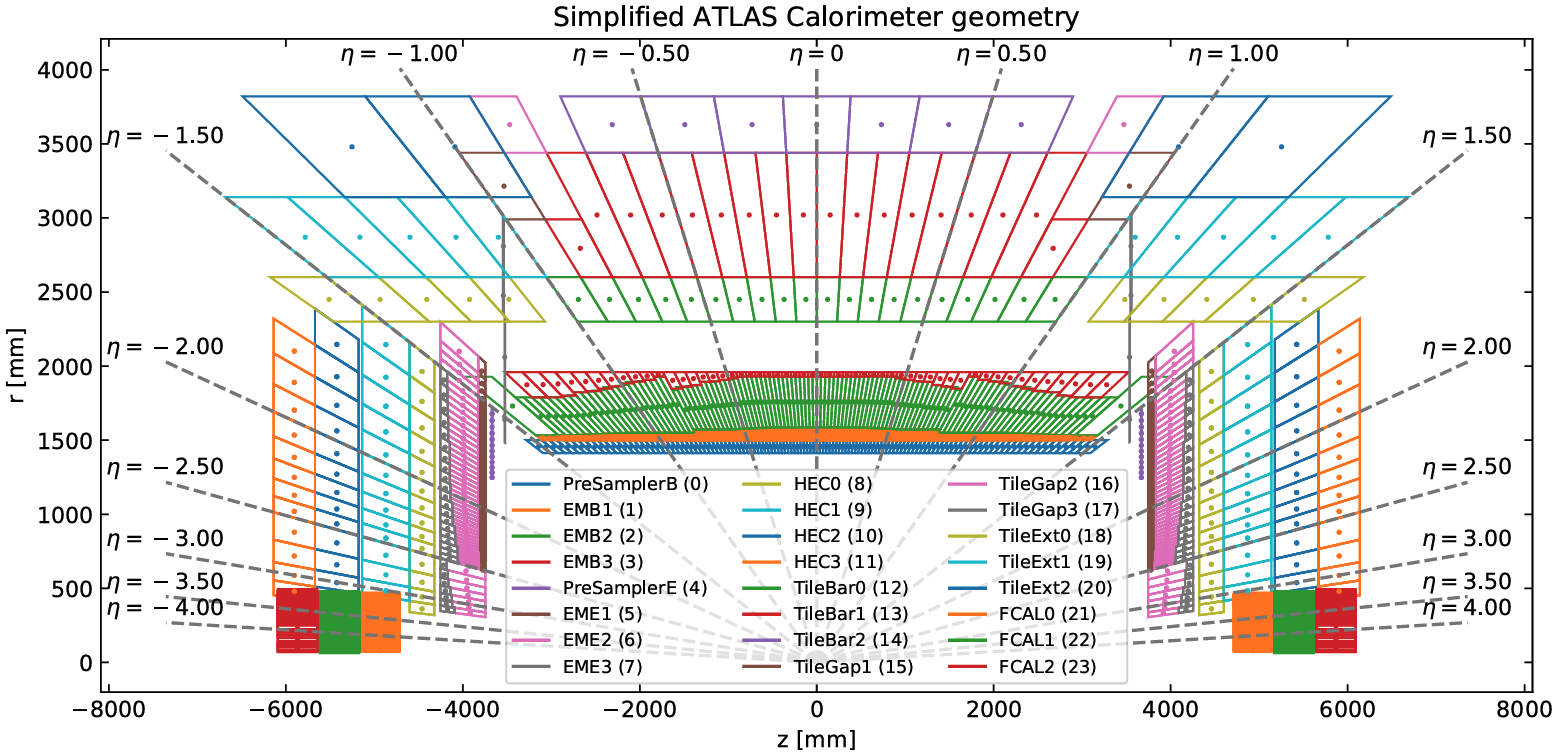
\includegraphics[width=0.9\linewidth]{cal_readout_ATLAS.png}
    \caption{Visualization of the ATLAS calorimeter readout geometry. The three subsystems, Tile, Liquid Argon and the Forward calorimeters, are shown~\cite{Gessinger:2752944}.}
    \label{fig:cal_resum}
\end{figure}

\vspace{-0.3}

Additional upgrades have also been implemented in the ATLAS calorimeter electronics to meet Run-3 conditions and to prepare for the forthcoming HL-LHC era, mirroring the improvements made to the Inner Detector and ensuring compatibility with the new trigger architecture. Both the Liquid-Argon and Tile Calorimeters have refurbished their on-detector and off-detector read-out chains; in TileCal specifically, new scintillating cryostat counters and renewed Minimum-Bias Trigger Scintillators have been installed for Run 3, enhancing electron-energy resolution and improving luminosity monitoring.

%xxxxxxxxxxxxxxxxxxxxxxxxxxxxxxxxxxxxxxxxxxxxxxxxxxxxxx
\subsection{Muon spectrometer}
\label{sec:muon}
%xxxxxxxxxxxxxxxxxxxxxxxxxxxxxxxxxxxxxxxxxxxxxxxxxxxxxx


Figure~\ref{fig:ms_atlas} shows the outermost subsystem of ATLAS, known as the Muon Spectrometer (MS)~\cite{mu_tech}. The MS is responsible for identifying muons, particles capable of traversing the calorimetric system with minimal energy loss. It comprises precision tracking chambers and fast-response trigger detectors embedded in a magnetic field of approximately 0.5~T in the barrel and 1.0~T in the end-cap regions, bending the trajectories of muons and enabling precise momentum measurement.

The MS includes four detector technologies totaling over one million readout channels. A schematic view of the subsystem is shown in Figure~\ref{fig:atlas_muon}, without including the New Small Wheel sector yet, implemented for Run~3. Two separate detector systems facilitate initial trigger decisions. Resistive Plate Chambers (RPCs) are used in the barrel region ($|\eta| < 1.05$), providing measurements with a resolution of about 10~mm in both longitudinal and transverse directions. In the end-cap region ($1.05 < |\eta| < 2.4$), Thin Gap Chambers (TGCs) handle higher background rates with wire separation of 1.8~mm and positional resolution around 5~mm. The RPC and TGC detectors primarily function as triggering components due to their fast response times.

Precision muon tracking relies mainly on Monitored Drift Tubes (MDTs), installed in both barrel and end-cap regions, covering the range $|\eta| < 2.7$ and offering high positional accuracy (approximately 35~µm per chamber). Cathode Strip Chambers (CSCs), multi-wire proportional chambers providing high rate capability and excellent time resolution (4~ns), are employed in the forward region ($2.0 < |\eta| < 2.7$). MDTs and CSCs are critical for accurately reconstructing muon trajectories.

For Run~3, the MS underwent significant upgrades, including the replacement of the forward muon-tracking region (known as the small wheel) with the New Small Wheel (NSW)~\cite{nsw_tech}. The NSW consists of two large 100-tonne detectors located at each end of ATLAS, each 10 metres in diameter and segmented into 16 sectors. The NSW employs advanced detector technologies such as Micromegas (MM) and small-strip Thin Gap Chambers (sTGC), capable of simultaneous precision tracking and triggering. Each wheel contains two layers of MM and sTGC chambers, resulting in four measurement planes for improved tracking accuracy and more than 2 million readout channels.
s
Moreover, despite being primarily designed to detect muons, the MS occasionally detects punch-through jets, hadronic jets that are not entirely absorbed by the calorimeters and reach the MS. The upgraded configuration of the MS, particularly with the addition of the NSW, significantly enhances ATLAS' capabilities in terms of tracking precision and trigger efficiency, essential for the high luminosity and challenging conditions expected during Run-3 and beyond.

Furthermore and aiming HL-LHC era, The Muon detectors will install new chambers in the barrel (RPCs and MDTs), replace the TGCs in the gap between the barrel and the end-caps and upgrade the readout electronics for the already installed RPCs, TGCs and MDTs to make them fully compatible with the trigger architecture.

\begin{figure}[htbp]
    \centering
        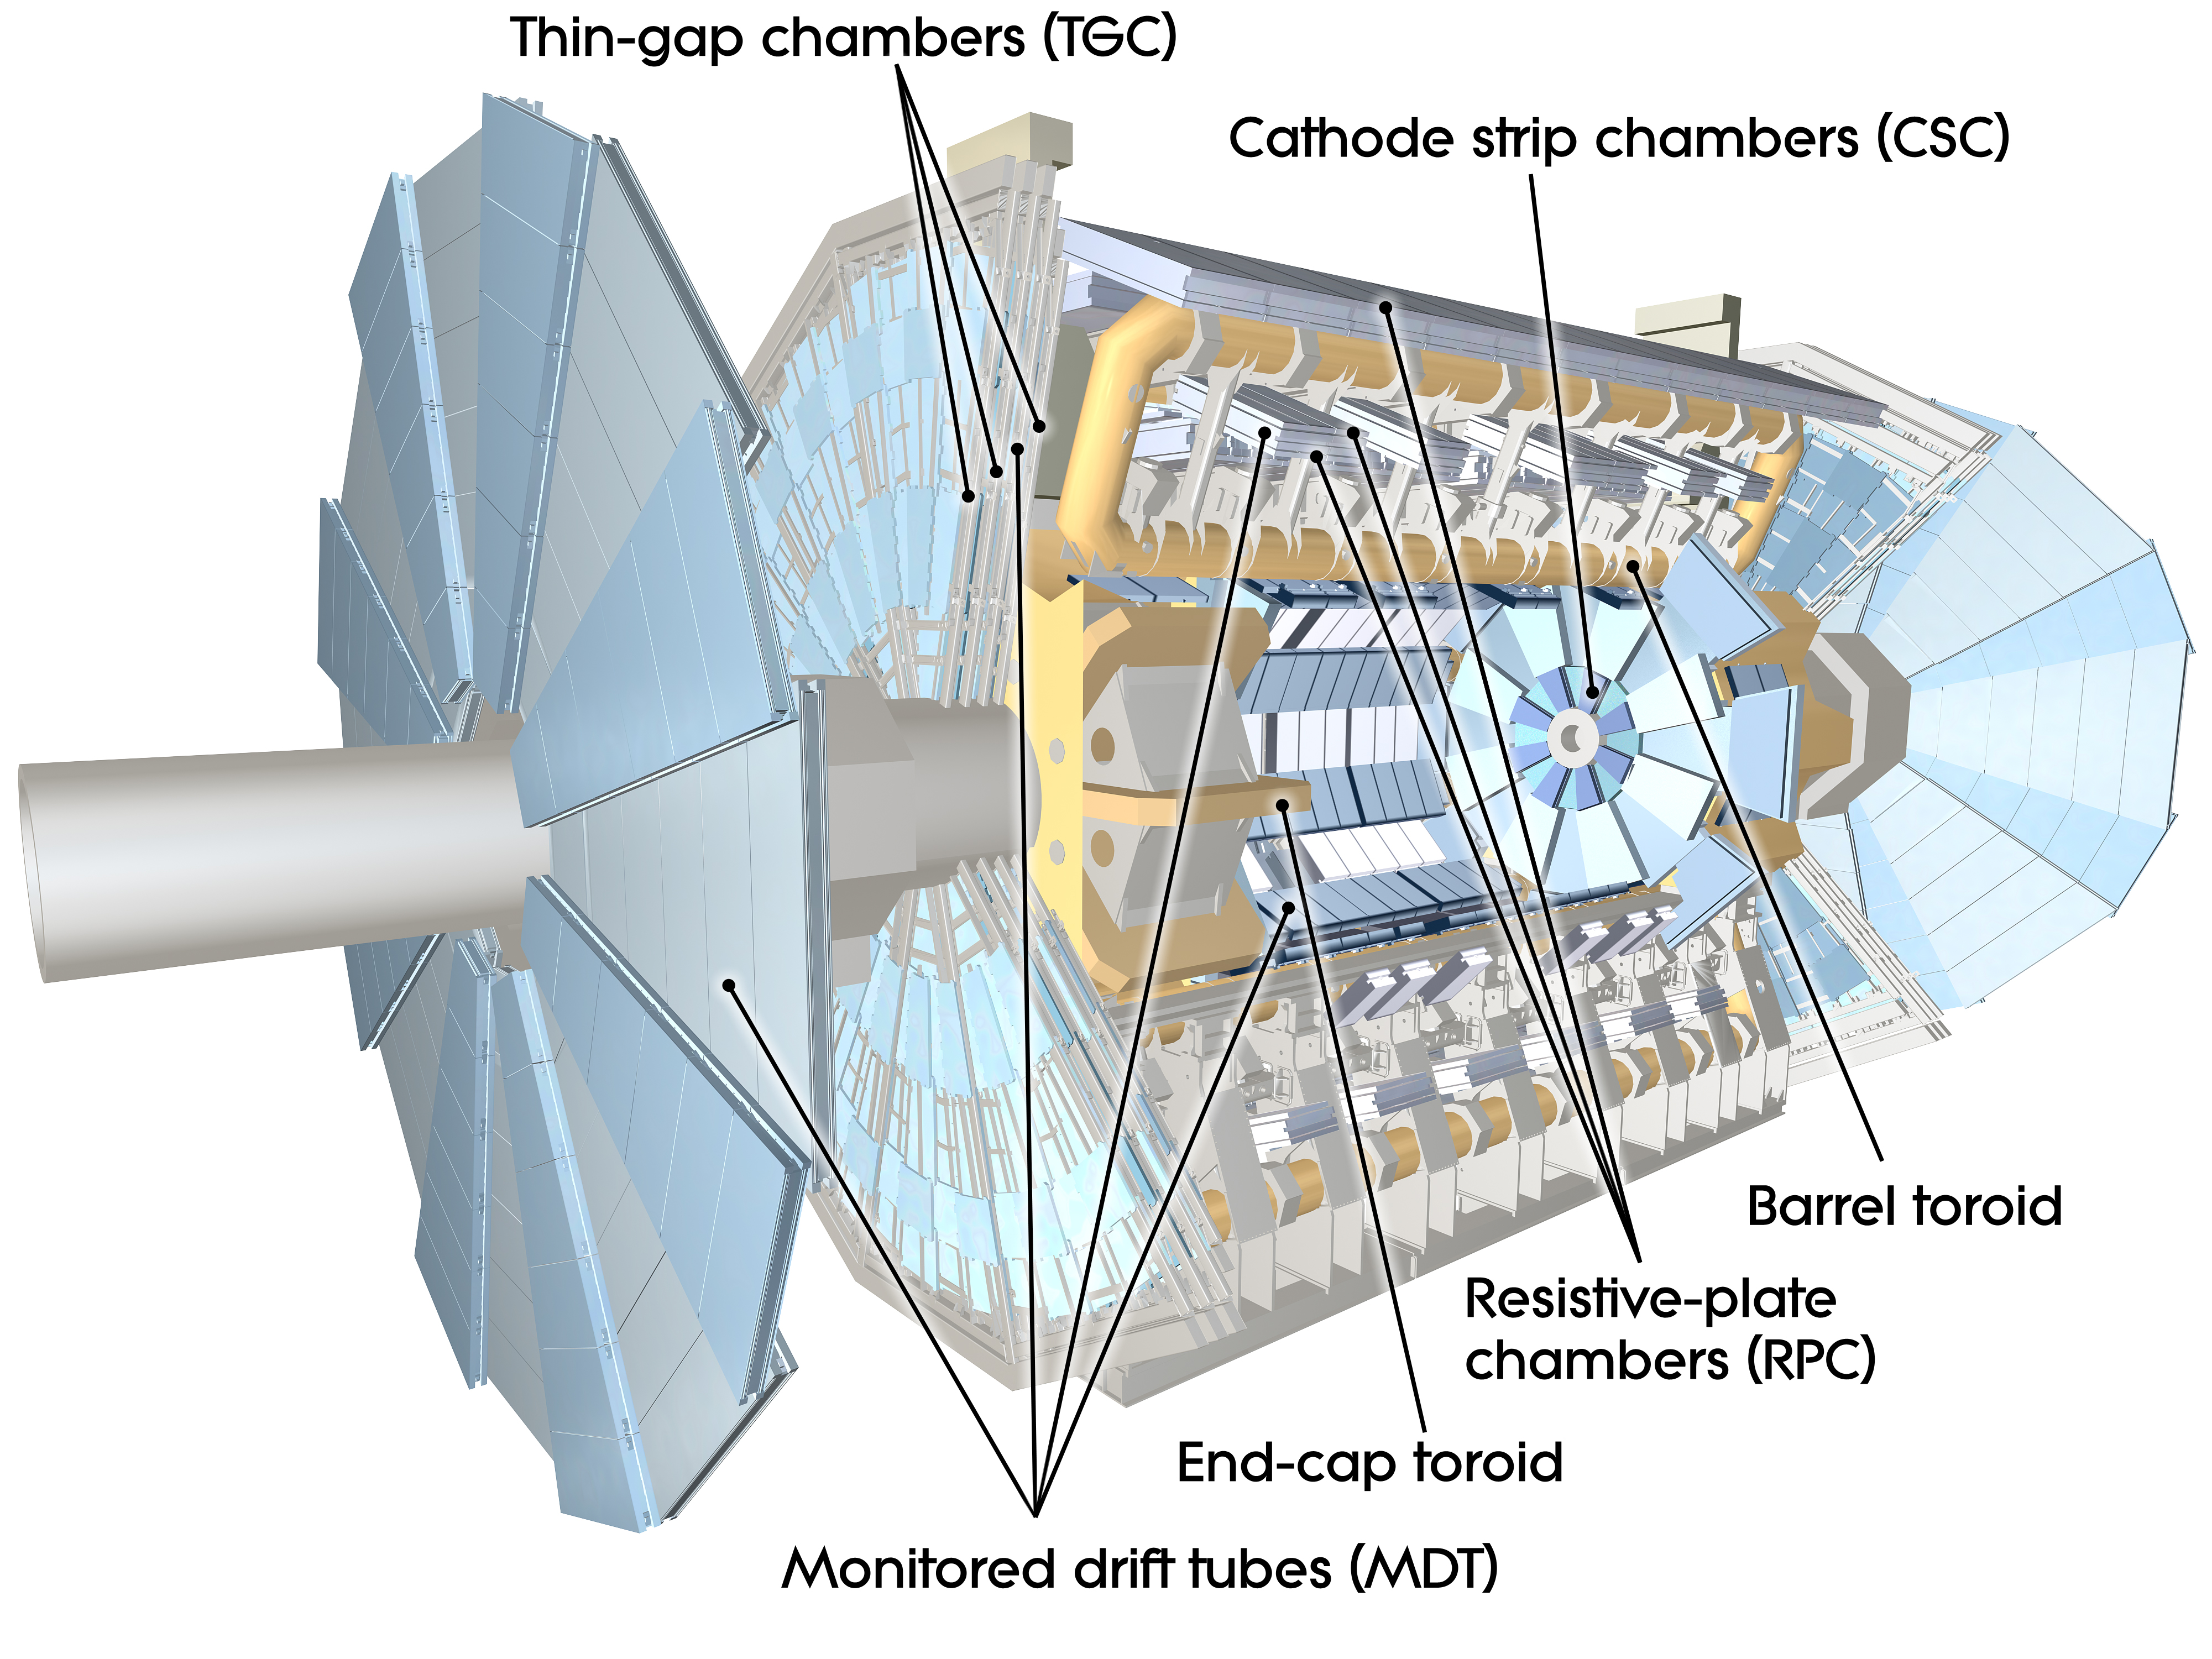
\includegraphics[width=0.9\linewidth]{ms_atlas.jpg}
    \caption{Cutaway representation of the ATLAS Muon Spectrometer~\cite{Bianchi:2837191}.}
    \label{fig:ms_atlas}
\end{figure}

%xxxxxxxxxxxxxxxxxxxxxxxxxxxxxxxxxxxxxxxxxxxxxxxxxxxxxx
\subsection{Forward detectors}
\label{sec:fwd}
%xxxxxxxxxxxxxxxxxxxxxxxxxxxxxxxxxxxxxxxxxxxxxxxxxxxxxx

Beyond the main subsystems listed above, ATLAS employs four compact forward subsystems covering the remaining region of the detector $(|\eta| > 5)$.
LUCID~\cite{Jenni:721908} (LUminosity Cherenkov Integrating Detector), situated $\pm17$ m from the interaction point, samples inelastic proton–proton interactions at very small angles and provides the experiment’s primary online and offline relative-luminosity measurement.  
LUCID is calibrated thanks to ALFA~\cite{Khalek_2016} (Absolute Luminosity For ATLAS), positioned inside Roman-pot stations $\pm240$ m from the IP, consists of scintillating-fibre tracking modules that can approach the beam to within $\sim\!1$ mm, enabling precise absolute-luminosity determinations and studies of elastic scattering.  
The AFP~\cite{Adamczyk:2015cjy} (ATLAS Forward Proton detector) was the last addition, located at 204 and 217 meters from the interaction point of both sides of the detector and aiming to extend the ATLAS physics reach by trying to tag very forward protons and enabling the observation of different processes where one of the two protons remains untouched.
Finally, the Zero Degree Calorimeter (ZDC)~\cite{Jenni:1009649}, installed $\pm140$ m from the IP, is built from alternating tungsten plates and quartz rods.  Covering $|\eta| > 8.3$, it detects neutral particles at zero degrees and is crucial for centrality measurements in heavy-ion collisions.

%xxxxxxxxxxxxxxxxxxxxxxxxxxxxxxxxxxxxxxxxxxxxxxxxxxxxxx
\subsection{Trigger, Data Acquisition and Detector Control Systems}
\label{sec:trigger}
%xxxxxxxxxxxxxxxxxxxxxxxxxxxxxxxxxxxxxxxxxxxxxxxxxxxxxx
One of the most demanding challenges for an experiment such as ATLAS at the LHC is to devise an efficient strategy for handling the enormous volume of data recorded in the tiny interval that follows each proton–proton collision. During routine LHC operation, proton bunches cross every 25 ns, yielding a raw collision rate of 40 MHz. Since each interaction produces thousands of particles,together with their consequent showers, a single fully digitised ATLAS event occupies roughly 1.5 MB, which would translate into a data stream of about 60 TB s$^{-1}$. Practical bandwidth and storage constraints therefore make it impossible to archive every event, and, in any case, the majority are not relevant to the core physics goals of the experiment. To curb this flood while retaining the maximum amount of useful information, ATLAS employs a dedicated trigger system~\cite{trigger_run2}. During Run 2 the trigger chain comprised two levels: a hardware–based Level-1 (L1) trigger, followed by a software–based High-Level Trigger (HLT). A schematic overview of the ATLAS Trigger and Data-Acquisition (TDAQ) system for Run 2 is shown in Figure~\ref{fig:trigger_system}.
\begin{figure}[htbp]
    \centering
        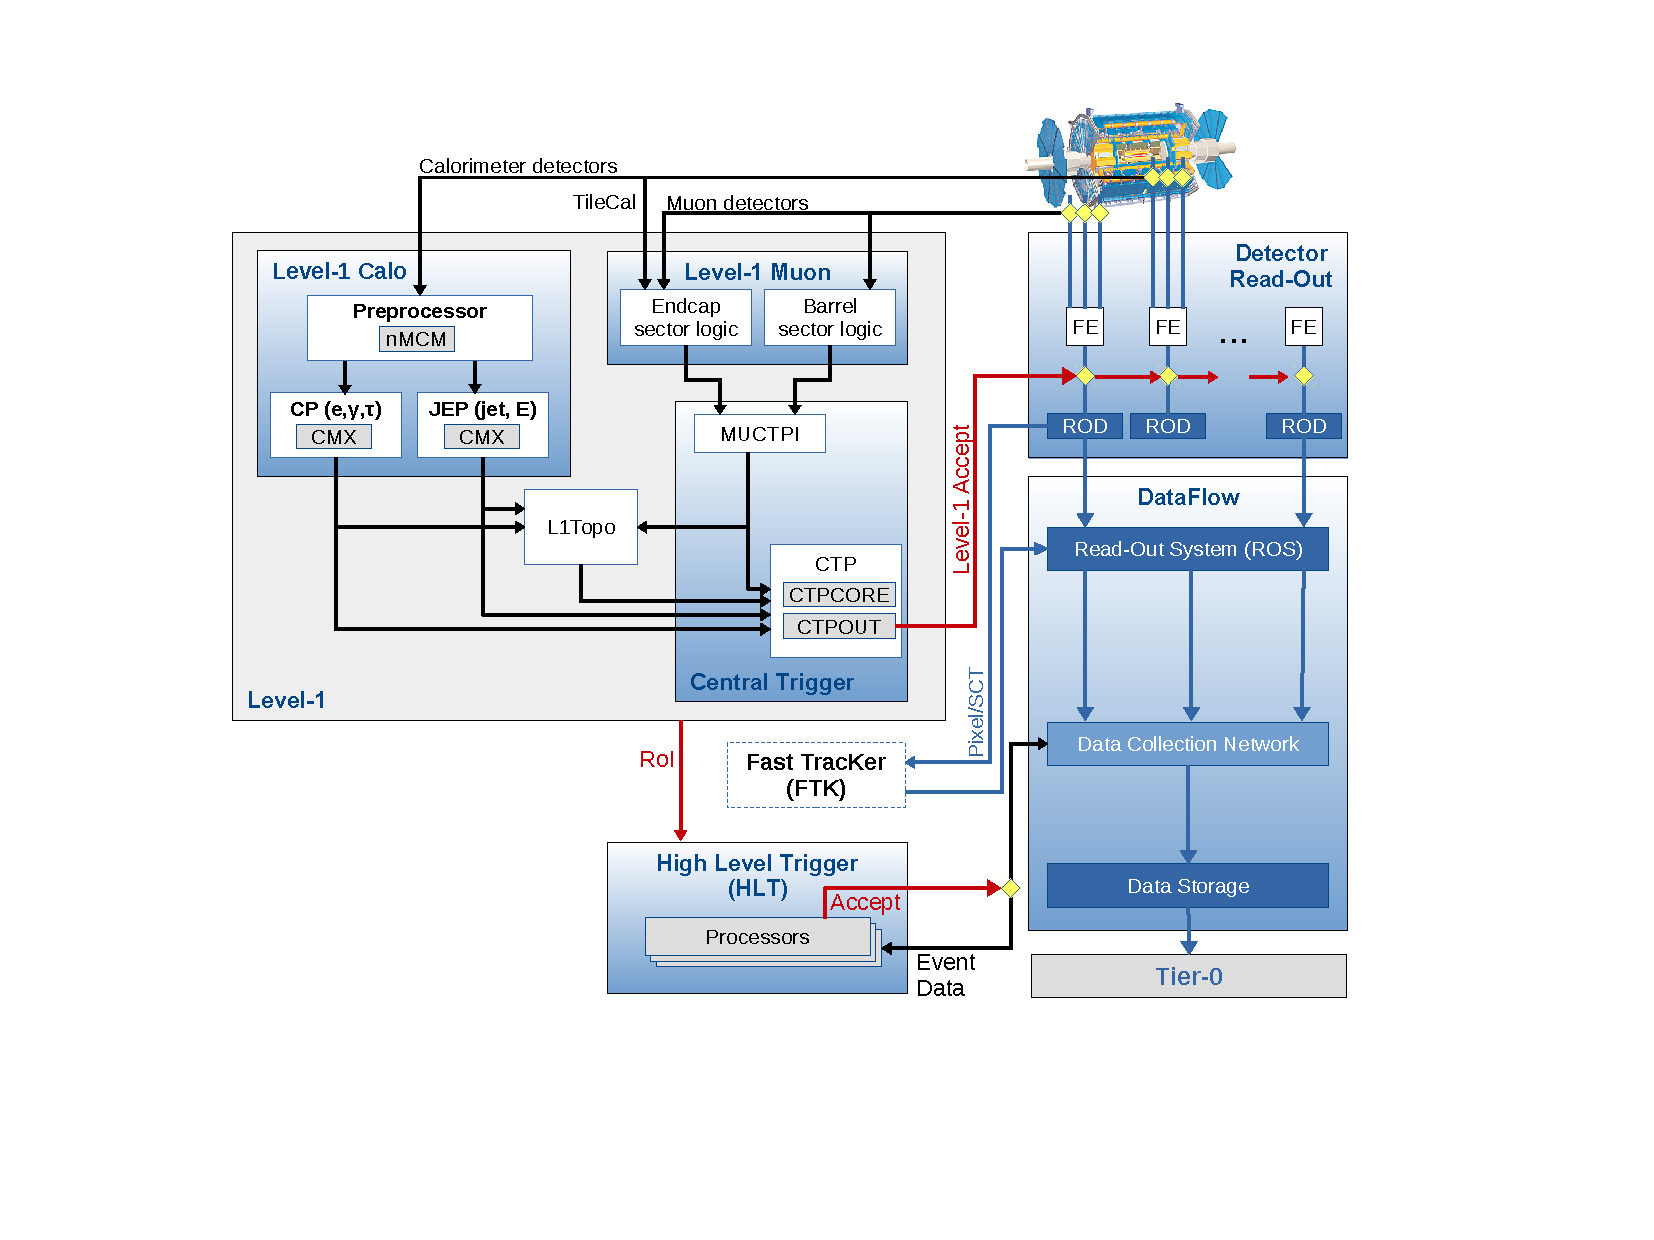
\includegraphics[width=0.9\linewidth]{tdaq-run2.pdf}
    \caption{Schematic of the ATLAS Trigger and Data Acquisition system in Run 2 with specific focus given to the components of the L1 Trigger system~\cite{atlas_daq_run2}.}
    \label{fig:trigger_system}
\end{figure}

The Level-1 trigger is a hardware-based system that cuts the raw 40 MHz collision rate down to about 100 kHz, operating with an exceptionally short latency of roughly 2.5 µs thanks to purpose-built custom and commercial electronics. The front-end electronics of every sub-detector store data in on-chip pipeline memories at the full 40 MHz bunch-crossing frequency. These buffers keep the digitised samples for ∼25 µs, that is the fixed window within which the L1 decision must be issued. That decision relies exclusively on information from the calorimeters and the muon spectrometer.

The L1 Calorimeter (L1Calo) trigger uses coarsened calorimeter read-outs (trigger towers) to locate regions of high energy deposition, i.e.\ regions of interest (RoIs). The L1 Muon (L1Muon) trigger exploits hits in the RPCs and TGCs to flag muon candidates, estimate their transverse momentum, and assign them to the correct bunch crossing. Outputs from L1Calo and L1Muon are merged in the Central Trigger Processor (CTP), which delivers the final verdict. If an event is accepted (an L1-Accept, or L1A), a signal is sent back to the front-end electronics so that the complete data corresponding to that bunch crossing can be read out from the pipeline memories. As noted above, the maximum L1A rate in ATLAS is 100 kHz.

The events accepted at Level-1 are first formatted by the sub-detector Read-Out Drivers (RODs) and then forwarded to the software-based High-Level Trigger (HLT). Running on a large computer farm, the HLT performs a rapid, partial reconstruction—tracking, charged-particle and jet identification (including $b$-jets), and a first estimate of the missing transverse momentum, throttling the event stream from \SI{100}{\kilo\hertz} to roughly \SI{1}{\kilo\hertz}. Events that satisfy these online selections are written to permanent storage and transmitted to CERN’s Tier-0 centre for full offline reconstruction. While awaiting the HLT verdict, the corresponding data fragments remain buffered in the Read-Out System (ROS).

During Long Shutdown 2 (LS2, between Run~2 and Run~3) the Phase-I upgrade preserved the two-level architecture while introducing a suite of crucial improvements. A fully digital L1Calo trigger path now feeds three FPGA-based feature extractors: eFEX for electrons and photons, jFEX for jets and missing transverse energy, and gFEX for global event variables. It uses super-cell granularity as fine as $\Delta\eta\times\Delta\phi = 0.025\times0.025$. In the forward region $(1.3<|\eta|<2.4)$ the newly installed New Small Wheels provide high-resolution muon trigger primitives, tightening transverse-momentum thresholds and cutting fake rates. The refurbished Level-1 Topological Processor exploits the finer calorimeter and muon inputs to impose angular, invariant-mass and transverse-mass selections in hardware. At the second stage, the HLT farm now runs on expanded computing resources, maintaining an output of roughly 3 kHz at an average event size of about 2.1 MB.

The Phase-II TDAQ upgrade, developed for the new conditions that will be delivered by HL-LHC, therefore foresees a two-stage hardware trigger in which an initial Level-0 decision accepts events at roughly \SI{1}{\mega\hertz}, followed by a refined Level-1 selection that throttles the rate to about \SI{400}{\kilo\hertz}. Both stages will exploit full-granularity calorimeter read-outs together with prompt track information from the new ITk. The latency budget will be stretched to $\sim!\SI{10}{\micro\second}$, and a trigger-less streaming DAQ is foreseen, capable of digesting data throughputs in excess of \SI{5}{\tera\byte\per\second}. An enlarged processing farm, augmented with hardware accelerators such as FPGAs and GPUs, will then filter the stream down to a sustainable output of \SIrange{10}{15}{\kilo\hertz} for permanent storage. Collectively, these upgrades will preserve and probably extend the experiment’s physics reach in the demanding high-pile-up environment of the HL-LHC.

\subsubsection*{Detector Control Systems}
A smooth dialogue between all ATLAS subsystems and the technical infrastructure that steers them is essential for reliable detector operation and data flow. This coordination is handled by the Detector Control System (DCS)~\cite{atlas_DCS}, which provides a unified interface for operators and continuously monitors voltages, temperatures, gas flows, and countless other parameters. Whenever an abnormal condition is detected, the DCS automatically issues alarms, attempts corrective actions where possible, and guides shifters through any manual interventions required. In addition, the DCS exchanges status flags with the DAQ so that data taking proceeds only when all components are in a safe, ready state, and it brokers communication among subsystems that are controlled independently.

\subsubsection*{The LHC computer grid}

To explain how the events accepted by the trigger are eventually processed, one must introduce The Worldwide LHC Computing Grid (WLCG)~\cite{Bird:1695401}, which is a global, tiered infrastructure that stores, distributes and processes the multi-petabyte data stream produced by the LHC experiments.  Data first reach Tier-0 at CERN, where the raw 40 MHz detector output is buffered, reconstructed and replicated; CERN then distributes this primary dataset to thirteen Tier-1 centres on three continents for large-scale reprocessing and long-term archival. Roughly 170 Tier-2 sites (university and regional clusters) supply the bulk of CPU for user analyses and Monte-Carlo production, while countless local Tier-3 farms serve individual groups.  
Today the WLCG federates $\sim$1.4 million CPU cores and $\sim$1.5 EB of disk and tape across 42 countries, sustaining average data‐transfer rates above 260 GB s$^{-1}$ and executing in excess of two million grid jobs daily.  This distributed model enables more than 12 000 physicists to access ATLAS data quasi-real-time, making large-scale analysis feasible without centralised super-computing resources.

%-------------------------------------------------------------------------------

%-------------------------------------------------------------------------------
\chapter{Event simulation}
\label{chap:dataset}
\newcommand{\MG}{\textsc{madgraph5}\xspace}
\newcommand{\MCNLO}{\textsc{mc@nlo}\xspace}
\newcommand{\aMCNLO}{\textsc{amc@nlo}\xspace}
\newcommand{\madgraph}{\textsc{madgraph5\_amc@nlo}\xspace}
\newcommand{\sherpa}{\textsc{sherpa}\xspace}
\newcommand{\OPENLOOPS}{\textsc{openloops}\xspace}
\newcommand{\powheg}{\textsc{powheg}\xspace}
\newcommand{\powhegbox}{\textsc{powheg-Box}\xspace}
\newcommand{\pythia}{\textsc{pythia}\xspace}
\newcommand{\herwig}{\textsc{herwig}\xspace}
\newcommand{\FxFx}{\textsc{FxFx}\xspace}
\newcommand{\MEPSNLO}{\textsc{MePs@NLO}\xspace}
\newcommand{\UNLOPS}{\textsc{UNLOPS}\xspace}
\newcommand{\MiNLO}{\textsc{MiNLO}\xspace}
\newcommand{\MADSPIN}{\textsc{MadSpin}\xspace}
\newcommand{\geant}{\textsc{Geant4}\xspace}
\newcommand{\afast}{\textsc{AtlFast-II}\xspace}
\newcommand{\evtgen}{\textsc{EvtGen}\xspace}
\newcommand{\toppp}{\textsc{Top}$_{++}$\xspace}
\newcommand{\COMIX}{\textsc{Comix}\xspace}
\newcommand{\PDFLHC}{\textsc{PDF4LHC}\xspace}
\newcommand{\tth}{\ensuremath{t\bar{t}H}\xspace}
\newcommand{\ctdiez}{\textsc{CT10NLO}\xspace}

\section{Proton-Proton event simulation}
\label{sec:event}

In this section, the modeling of proton-proton collisions occurring at the LHC is presented, which comprises several stages~\cite{BUCKLEY2011145}.
Firstly, the production cross-section for the hard scattering introduced previously in Section~\ref{subsec:proton} is calculated, describing the interactions between the partons that compose the incoming protons.
This is followed by parton showering, where gluon emissions and parton splitting are simulated. The next step involves hadronization, where resulting partons combine to form color-neutral hadrons, which subsequently decay along with other unstable particles. Additionally, the modeling of pile-up and underlying events, originating from multiple simultaneous proton interactions beyond the primary scattering within the same bunch crossing, is included.
Finally, events undergo detector simulation, digitization, and the same reconstruction algorithms used for real data, ensuring a realistic representation of experimental conditions.
Figure~\ref{fig:pdfs} illustrates the aforementioned steps involved in simulating a proton-proton collision.
\begin{figure}[htbp]
    \centering
    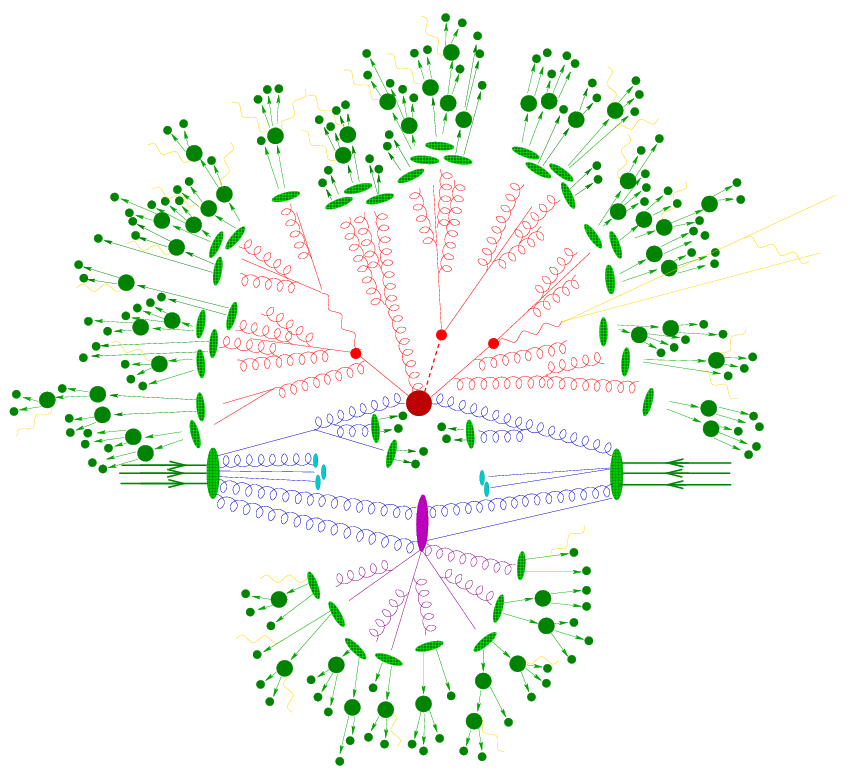
\includegraphics[width=0.9\textwidth]{images/atlas_pp_sim.png}
    \caption{Representation of components relevant for simulating a proton-proton collision event containing all the factorised stages, excluding pile-up~\cite{Gleisberg_2009}. The central red blob represents the hard-scattering of incident protons,
    while in blue it shows the initial partons that contributed. Additional hard QCD radiation, outgoing partons and their decays are also represented in red. In light green ellipses it is represented the hadronization of final state partons, while the decay
    of the resulting hadrons is represented by dark green regions with arrows. The partons that did not participate in the primary interaction conform the underlying event, in purple. In yellow one can find the photon radiation, that can occur at any stage.}
    \label{fig:pdfs}
  \end{figure}

\subsection{Matrix element and parton showers}
\label{subsec:parton_shower}
Given the large momentum transfer involved in the hard scattering processes at the LHC, the partonic cross-sections can be computed using perturbative QCD. In this framework, partons may radiate additional gluons and split into quarks, which in turn can emit yet more radiation both in the initial and final states. Computing the full cross-section ($\hat{\sigma})$ therefore requires summing over all possible quark/gluon emissions, which can be expressed as the perturbative expansion:
\begin{equation}
\hat{\sigma}(ij\rightarrow X) = \sum_{n=0}^{\infty}\int d\Phi_{X+n}\abs{\sum_{k=0}^{\infty}|\mathcal{M}_{X+n}^{^{(k)}}}|^2,
\end{equation}
being $\mathcal{M}_{X+n}^{^{(k)}}$ the matrix element for the process $ij \rightarrow X + n$, with $n$ the number of additional partons produced in the final state, $k$ the number of included virtual loops, and $d\Phi_{X+n}$ the phase space element for this process.
The calculation at LO only includes tree level matrix elements so it would correspond to $n=0$ and $k=0$. If the process involves the production of $N$ partons in the final state, then in this case the LO calculation for the process $ij \rightarrow X+N$ will involve $n=N$ and $k=0$.
In the same way, a matrix element calculation with $k + n = m$ is referred to as a calculation at $\text{N}^{\text{m}}$LO, for $ij \rightarrow X$.

This is how the cross-sections are calculated precisely for such scattering processes. However, when too many partons appear in the final state the computation becomes prohibitively expensive, so the matrix elements are evaluated only up to a certain order in the strong coupling constant
 $\alpha_{s}$ (see Eq.~\ref{running}), and the remainder is approximated via the parton-showering algorithm, where the showering is simulated using approximate matrix elements~\cite{FOX1980285}.

%%Because parton emissions span a wide range of energy scales, the phase space accessible to a parton-shower algorithm inevitably overlaps with that already covered by higher-multiplicity matrix elements. If left untreated, this overlap would double-count contributions and decrease the accuracy of cross-section and jet-multiplicity predictions, especially when an energetic, wide-angle emission converts an n-jet configuration into an (n + 1)-jet one.
%%Matching and merging prescriptions resolve the overlap by defining, event-by-event, which emissions originate from the fixed-order calculation and which from the shower. Slicing techniques introduce a matching scale: high-pT, large-angle partons are described by multi-leg matrix elements, while softer or more collinear radiation is delegated to the shower, preserving leading-logarithmic accuracy without duplication. Widely used implementations include 
%%the geometrical MLM~\cite{MANGANO2002343} algorithm and the CKKW~\cite{Catani_2001} schemes, which re-weight matrix elements and constrain subsequent showering; their next-to-leading-order extension is known as FxFx~\cite{Frederix_2012}. By combining samples of increasing jet multiplicity under these rules, one obtains inclusive event samples that smoothly interpolate between the hard and soft regimes.
Matching and merging schemes prevent double counting between high-multiplicity matrix elements and the parton shower by assigning emissions above a chosen matching scale to fixed-order calculations and relegating softer or collinear radiation to the shower. Widely used approaches, such as the MLM algorithm~\cite{MANGANO2002343} and CKKW schemes~\cite{Catani_2001} with their NLO extension FxFx~\cite{Frederix_2012}, combine tree-level multileg samples
of increasing jet multiplicity with parton showers to produce inclusive event samples that smoothly interpolate between hard, wide-angle emissions and soft, collinear radiation.

\subsection*{Hadronization}
\label{subsec:Hadronization}

Below the perturbative cutoff of order 1 GeV, parton showering hands off to non-perturbative hadronization, during which coloured partons (each carrying definite momentum, flavour and colour) are clustered into colour-neutral hadrons. Phenomenological models such as the Lund string model or the cluster model take over here.

In the Lund string model~\cite{ANDERSSON198331} the colour field between a quark and an antiquark is treated as a relativistic string whose potential energy rises with separation; when that energy exceeds the mass of a new $q\bar{q}$ pair the string breaks, repeatedly creating additional pairs until all energy is exhausted, with hadron momenta drawn from an empirical fragmentation function. 
The cluster model~\cite{Winter_2004} instead splits each final-state gluon into a $q\bar{q}$ pair and groups them into colour-singlet clusters; those clusters then undergo a cascade of decays, or directly fragment, until only stable hadrons remain.

\subsection*{Pile-up and underlying event}
\label{subsec:Pile}

All activity and interactions occurring in a proton-proton collision beyond the primary hard scattering must also be modelled; these are referred to as the underlying event and pile-up backgrounds, as discussed in Section~\ref{sec:LHC}. 
In the case of the underlying event, the soft interactions between partons are mainly described using phenomenological models, given their non-perturbative nature. When considering pile-up, one must simulate the additional proton-proton interactions that occur alongside the hard scattering, arising from nearby bunch crossings or even from protons interacting with beam-pipe or detector components.

Each of these effects is generated separately and then overlaid onto the hard-scattering event before passing the combined event through the full detector simulation.



\section{Detector response simulation}
\label{sec:Detector}

The raw collision data recorded by ATLAS arise solely from the interactions of final-state particles with the various subdetectors (see Section~\ref{sec:ATLAS}). To compare our Monte Carlo predictions with real data, each simulated event is propagated through a detailed detector model and reconstruct it identically to the collision data.  This full detector simulation is performed with the \textsc{Geant4} toolkit~\cite{AGOSTINELLI2003250}, which tracks particles through the precise geometry of every ATLAS subsystem, simulates their electromagnetic and hadronic interactions, and converts energy deposits and tracks into digitized detector signals.

For maximum accuracy one employs the “Full Simulation” procedure in which \textsc{Geant4} processes the complete ATLAS geometry.  However, calorimeter showers dominate the CPU cost, consuming nearly 90\% of the resources.  To speed up large-scale productions, the \textsc{AtlFast-II} fast-simulation simplified framework~\cite{Edmonds:1091969,ATLAS:1300517} applies parametrized responses for both the inner detector and calorimeters, reducing computing time by an order of magnitude.  Lastly, all simulations incorporate the actual detector conditions in force at the time of production: dead channels, electronic noise, alignment shifts, and calibration constants. Therefore the simulated events can always contain some mismatch with the real data, since the conditions of the detector change constantly during the data taking.


\section{Monte Carlo simulation generators}
\label{sec:mc}
Monte Carlo generators are basically software tools that use pseudorandom numbers to reproduce predicted kinematic distributions and event dynamics for a given physics process according to a theoretical model such as the SM.  They fall into two broad classes: general-purpose generators, which reproduce the entire chain of event generation (hard scattering, parton showering, hadronization, etc.), and more specialized codes that excel at specific tasks, for example high-order matrix-element computations or detailed modeling of parton cascades.

To emulate the entire physics process of an event, several MC generators are commonly used. From a more generic approach to a more specialised one, we find \pythia~\cite{SJOSTRAND2015159}, which is a general-purpose generator.
This software uses LO matrix element calculations for $2 \rightarrow n$ events with up to three final-state partons, incorporating a $p_{\text{T}}$-order parton shower, based on the Lund model for hadronisation. Although this approach is capable of modelling the soft and hard interactions of the collision, its purely at LO cross-section is often not sufficient for high-precision analyses, so it must often be combined with other higher-order matrix element generators, and is used only as a parton shower generator.

Another generator with similar capabilities but which focuses on an angular-ordered parton shower is \herwig~\cite{B_hr_2008}. It offers only $2 \rightarrow 2$ LO matrix element calculations and takes into account gluon splitting by incorporating all spin correlations, something that \pythia does not do. This software can simulate 
a wide range of processes with NLO accuracy for the matrix element calculation, but results in many events with negative weight which is problematic at certain stages of the physics analysis such as the one presented in this thesis. It is therefore also interfaced with other software that provides matrix element calculation at higher orders, while this one is used for hadronization, employing a cluster model.

\sherpa~\cite{Bothmann_2019} is another MC generator which uses the CKKW matching procedure~\cite{Lavesson_2008} to move from matrix element calculation, at LO and NLO, to parton showering modelling, operating for processes with multiple partons. It uses the cluster model for hadronization, and produces quite accurate simulations especially for processes with multiple jets or electroweak bosons. 
If interested in more precise high-order matrix element calculations, the most commonly used algorithm is \madgraph~\cite{Alwall_2014}. It uses \textsc{MC@NLO} method to interface with parton showers, using MLM~\cite{MANGANO2002343} and FxFx~\cite{Frederix_2012} matching models. It is usually used in conjuction with \pythia or \herwig.

Finally, the \powhegbox~\cite{Frixione_2007} framework is also widely employed for high-order matrix element calculations, especially consistent for dealing with QCD corrections in both matrix elements and parton showers.

\section{Data and MC simulated samples}
\label{sec:mc_samples}

All studies discussed in this thesis depend critically on comprehensive Monte Carlo simulations of both signal and background processes. These simulated samples provide the expected event yields and model the detector’s response, incorporating the latest fixed-order 
theoretical cross-section calculations, state-of-the-art parton-distribution functions, and full event-generation chains including parton-shower evolution and hadronization. In the Higgs boson analyses presented here, the signal datasets reproduce the dominant production modes, while the background samples cover the SM processes most likely to mimic those signatures.

For the electron-identification performance studies, dedicated simulations are used to model prompt electrons from $Z \rightarrow e^{+}e^{-} $ y $J/\psi \rightarrow e^{+}e^{-}$ decays, as well as non-prompt electrons arising from other heavy-flavor decays or misidentified objects. The following sections describe the choice of generators and specific configuration settings employed
to simulate each signal and background process in these analyses.

\subsection{Simulation samples for electron studies}
\label{subsec:electron_mc}
As mentioned above, studies regarding electron identification presented in this thesis (Chapter~\ref{chap:electrons}) use MC simulation selecting electrons from $Z \rightarrow e^{+}e^{-} $ and $J/\psi \rightarrow e^{+}e^{-}$ processes.
Regarding background samples, we consider both $2 \to 2$ QCD multijet production and $t\bar{t}$ pair decays.

Both the signal and background events are processed through the full ATLAS detector simulation.
The \powhegbox~v1 matrix-element generator\ provides the hard-scattering simulation at NLO accuracy for $Z$-boson production and decay in the electron channel.  Parton showering, hadronisation and underlying-event modelling are handled by \pythia~8.186, employing the \textsc{aznlo} tune. The \textsc{ct10nlo} PDF set is used for the hard scattering, while \textsc{cteq6l1} is adopted for the showering.
Final-state-radiation effects are incorporated with \textsc{photos++}\,3.52~\cite{davidson2015photosinterfacectechnical,Golonka_2006}.  Bottom- and charm-hadron decays are simulated with \textsc{evtgen}1.2.0~\cite{LANGE2001152}.

Prompt $J/\psi\!\to e^{+}e^{-}$ samples are generated with \pythia8.186 using the A14 tune~\cite{A14} together with the \textsc{cteq6l1} PDF set. A tune refers to a specific set of Monte Carlo generator parameters adjusted to produce the data, with the A14 tune being one of the standard ATLAS tunes for underlying-event modelling.

Additional background $2\!\to\!2$ QCD processes that mimic the prompt-electron signature are modelled with \pythia8.186 (A14 tune) and the \textsc{nnpdf}-\\{\small2.3}\textsc{lo} PDF set. 
These samples, commonly referred to as JF17, are obtained by filtering events to reproduce the highly localised energy deposits characteristic of electrons, requiring particles (excluding muons and neutrinos) produced in the hard scatter to have a summed transverse energy exceeding 17~GeV within an area of $\Delta\eta \times \Delta\phi = 0.1 \times 0.1$. 
They cover multijet production, $qg\rightarrow q\gamma$, $q\bar{q}\rightarrow g\gamma$, electroweak $W$ and $Z$ production, and top-quark processes, thereby providing mainly background electrons that imitate prompt signatures.

Top-quark pairs are modelled with \powhegbox v2 at NLO using the \textsc{nnpdf3.0nlo} PDF set, with $h_{\text{damp}}$ $=1.5\,m_{\text{top}}$~\footnote{The $h_{\text{damp}}$ parameter is a resummation damping factor that controls the matching of the matrix element calculation with the parton showering (and consequently the amount of high-pT radiation against the $t\bar{t}$ system recoil)~\cite{hdamp}}.
Parton shower, hadronisation and underlying event are provided by \pythia8.230 (A14 tune, \textsc{nnpdf2.3lo} PDFs), while heavy-flavour decays are handled by \textsc{evtgen}\,1.6.0.  At least one $W$ boson from the $t\bar t$ decay chain is required to decay leptonically.

Multiple $pp$ interactions in the same or neighbouring bunch crossings are simulated by overlaying each hard-scatter event with minimum-bias interactions produced with \pythia~8.186.

\subsection{Higgs boson and backgrounds simulated samples}
\label{subsec:higgs_mc}

\subsubsection*{Simulation of Higgs boson samples}
Apart from electron performance studies, the analysis that will be discussed in this thesis (Chapters~\ref{chap:htautau},~\ref{chap:run3_tth}) consider the main production modes of the Higgs boson in the LHC, already introduced in Section~\ref{sec:higgs_program}. 

In the case of the leading production mode, ggF, the samples are produced at NNLO in QCD using \powheg NNLOPS, and scaled to the cross-sections computed at $\text{N}^{3}$LO in QCD~\cite{PhysRevLett.114.212001,anastasiou2016,Harlander_2009,Harlander,Harlander_2010,Pak_2010}, including NLO electroweak corrections~\cite{Actis_2008,Bonetti_2018}.
These samples are obtained using the \textsc{pdf4lhc15nlo} PDF set~\cite{Butterworth_2016} together with the \textsc{AZNLO} tune for \textsc{pythia8} for the parton showering and hadronization. 

The event samples for VBF production mode are generated at NLO with \powheg interfaced with \pythia~8. The \textsc{AZNLO} tune is also used here for the showering and hadronization and the \textsc{pdf4lhc15nlo} PDF set for the PDFs. Again, the predicted samples are scaled to the cross-section computed at an approximate NNLO in QCD~\cite{Bolzoni_2010}, including EW corrections as well at NLO level~\cite{Ciccolini_2008}.

The Higgs boson production in association with a vector boson is simulated at  NLO with one additional parton using \powheg interfaced with \textsc{pythia8}. Once again, \textsc{AZNLO} tune is used for the parton showering and hadronization,
and the \textsc{pdf4lhc15nlo} PDF set is used for the PDFs. The gluon-induced production of the Higgs boson in association with a vector boson is generated at LO with the same setup. 
For the quark-induced production, a normalization to the NNLO computation in QCD is applied, including NLO electroweak corrections, and to the NLO computation in QCD for the gluon-induced production~\cite{Ciccolini_2003,Denner_2015,Harlander_2014,Altenkamp_2013,Brein_2012, Harlander_2018, Brein_2013}.

For the \tth production mode, the \powhegbox v2 generator at NLO in QCD~\cite{frixione2015,Zhang_2014,Dawson_2003,Beenakker_2003} is used, configured with the \textsc{nnpdf3.0nlo} PDF set~\cite{Martin_2009}, interfaced with A14 tune of \pythia8.230 for the parton shower modeling~\cite{A14}. The simulation of bottom decay is generated using \evtgen v1.6.0~\cite{LANGE2001152}.
In the case of the production associated to a single top quark, it is modeled at NLO using \madgraph, interfaced with \pythia8, with the \textsc{CT10} PDF set and A14 tune. These samples are subsequently normalized to NLO in QCD computed cross-section.

In all these cases, in order to estimate the uncertainties due to the choice of the parton showering and underlying event modeling, an alternative sample is generated using \textsc{Herwig7} for the parton showering and hadronization, 
but keeping the matrix element calculation with \powheg. Similarly, to estimate the uncertainties due to the choice of the generator for the matrix element calculation,
an alternative sample is generated using \madgraph interfaced with \textsc{pythia8}, and \textsc{Herwig7}~\cite{bellm2017herwig71releasenote} for the parton showering and hadronization.
In Table~\ref{tab:MC_samples} a summary of nominal MC generators employed for each process can be found.

As the last step, the branching ratios for the Higgs boson decays are computed using the \textsc{hdecay}~\cite{Djouadi:1997yw,Spira:1997dg,Djouadi:2006bz} and \textsc{prophecy4f}~\cite{Bredenstein:2006ha,Bredenstein:2006rh,Bredenstein:2006nk}.
The full normalization of signal samples integrates the branching ratio of the Higgs boson decays to the pair of $\tau$-leptons considered in this analysis. In order to compute the calculate the cross-sections and branching ratios, the Higgs boson mass is set to 125.09~GeV.

Everything shown above mainly describes the simulations used for the first round of the Run-2 analysis (using the MC16 production campaign in rel.21) presented in this thesis. In order to simulate the physics events produced during in the rel.22 MC20 (Run 2) and MC23 (Run 3) campaigns,
the combinations of MC generators, PDF sets and tunes generally remain the same as those detailed in Table~\ref{tab:MC_samples}, unless otherwise stated.

For this new simulation campaign \powheg is still used together with \pythia for the matrix-element calculation and parton-shower description, but with more up-to-date versions (v6 and later releases of \pythia8), also for Higgs production in association with a single top quark ($tH$), encompassing both $tHqb$ and $tWH$.
Regarding the tune sets for the PDFs, this new round employs A14 together with \textsc{nnpdf2.3lo} for all of them, whereas in the first Run-2 round \textsc{CTEQ6L} and \textsc{AZNLO} tunes were also used for hadronization and showering.

\subsubsection*{Simulation of background samples}

The QCD $W/Z$+jets ($V$+jets) background is modelled with \sherpa v2.2.1 at NLO for up to two extra partons, using the \textsc{nnpdf3.0nnlo} PDF set.  Matrix elements with up to four additional partons are generated at LO via the \textsc{comix}~\cite{Gleisberg_2008} and \textsc{openloops}~\cite{Buccioni_2019,Cascioli_2012,Denner_2017} libraries, and merged with the parton shower using the \textsc{meps@nlo} scheme of \sherpa.  The yields are normalized to NNLO cross-section predictions.  
Electroweak \(V\)+jets samples are produced with the same setup (\textsc{sherpa} v2.2.1 + \textsc{nnpdf3.0nnlo} + \textsc{meps@nlo}).

\(\ttbar\) events are generated in following the same strategy as explained before in Section~\ref{subsec:electron_mc}, with the difference that in this case we do not restrict to events where at least one of the $W$ bosons from the \(\ttbar\) system decays leptonically.

Single-top \(s\)- and \(t\)-channel processes are generated at NLO in QCD with \powheg v2 using \textsc{nnpdf3.0nlo}, in the five- and four-flavour schemes respectively, and parton showers modeled with \textsc{pythia8} 2.30 (A14 + \textsc{nnpdf}2.3\(\text{lo}\)).  Cross-sections are normalized to NLO predictions from \textsc{hathor} 2.1~\cite{Aliev_2011}.  

Diboson (\(WW\), \(WZ\), \(ZZ\)) samples are simulated with \sherpa v2.2.1-2.2.2, with NLO matrix elements for up to one extra parton and LO for up to four.  Gluon-induced \(gg\to VV\) is included at LO (up to one extra parton).  Merging is performed via \textsc{meps@nlo}, using the \textsc{nnpdf}3.0\textsc{nnlo} set, and virtual QCD corrections are provided by \textsc{OpenLoops}.  All diboson samples are normalized to NLO cross-sections.  

In the MC20/MC23 campaigns (rel.22), only the generator versions, merging multiplicities and normalizations have been updated: \sherpa for $V$+jets is now v2.2.14 with NLO up to two and LO up to five extra partons under an improved \textsc{ckkw}-\textsc{meps@nlo} merge; 
\ttbar and single-top remain generated with \powhegbox v2 but are showered with \textsc{pythia}8.308 (A14, \textsc{nnpdf2.3,lo}) and use \textsc{evtgen}2.1.1, with normalization to the NNLO+NNLL cross-section from \textsc{top++,2.0}/\textsc{pdf4lhc21}; dibosons are produced with \sherpa 2.2.14 (NLO up to one, LO up to three extra partons, including \(gg\to VV\) at LO) merged via \textsc{ckkw}-\textsc{meps@nlo} and normalized as before.

\begin{sidewaystable}[p]
  \centering
  \small
  \caption{Summary of the MC generators employed in rel.21 for the primary signal and background samples. Normalization indicates the perturbative order used in the cross-section calculations for each sample.}
  \label{tab:MC_samples}
  \begin{tabular}{l ll ll ll}
    \toprule
    Process & \multicolumn{2}{c}{Generator} & \multicolumn{2}{c}{PDF set} & Tune & Normalization \\
    \cmidrule(lr){2-3} \cmidrule(lr){4-5}
            & ME & PS & ME & PS & & \\
    \midrule
    \multicolumn{7}{l}{\textbf{Higgs boson}} \\
    ggF        & \powhegbox v2       & \pythia 8        & PDF4LHC15\textsc{nnlo} & CTEQ6L1    & AZNLO & N$^3$LO QCD + NLO EW \\
    VBF        & \powhegbox v2       & \pythia 8        & PDF4LHC15\textsc{nnlo} & CTEQ6L1    & AZNLO & NNLO QCD + NLO EW   \\
    $VH$       & \powhegbox v2       & \pythia 8        & PDF4LHC15\textsc{nnlo} & CTEQ6L1    & AZNLO & NNLO QCD + NLO EW   \\
    $t\bar tH$ & \powhegbox v2       & \pythia 8        & NNPDF3.0\textsc{nlo}   & NNPDF2.3\textsc{lo} & A14   & NLO QCD + NLO EW    \\
    $tH$       & MadGraph5\_aMC@NLO & \pythia 8        & CT10          & NNPDF2.3\textsc{lo} & A14   & NLO                 \\
    $b\bar bH$ & \powhegbox v2       & \pythia 8        & NNPDF3.0\textsc{nnlo}  & NNPDF2.3\textsc{lo} & A14   & NLO                 \\
    \midrule
    \multicolumn{7}{l}{\textbf{Background}} \\
    $V$+jets    & \sherpa v2.2.1      & \sherpa         & \multicolumn{2}{c}{NNPDF3.0\textsc{nnlo}} & \sherpa & NNLO (QCD), LO (EW) \\
    $t\bar t$  & \powhegbox v2       & \pythia 8        & NNPDF3.0\textsc{nlo}   & NNPDF2.3\textsc{lo} & A14   & NNLO + NNLL         \\
    Single top & \powhegbox v2       & \pythia 8        & NNPDF3.0\textsc{nlo}   & NNPDF2.3\textsc{lo} & A14   & NLO                 \\
    Diboson  & \sherpa v2.2.1      & \sherpa         & \multicolumn{2}{c}{NNPDF3.0\textsc{nnlo}} & \sherpa & NLO                 \\
    \bottomrule
  \end{tabular}
\end{sidewaystable}
  
  


    
    
%-------------------------------------------------------------------------------

%-------------------------------------------------------------------------------
\chapter{Physics objects reconstruction}
\label{chap:object_rec}
\newcommand*{\antikt}{anti-$\kappa_{t}$\xspace}
\newcommand*{\et}{$E^{\text{miss}}_{\text{T}}$\xspace}
\newcommand*{\tauhadvis}{$\tau_{\text{had-vis}}$\xspace}
\newcommand*{\tauhad}{$\tau_{\text{had}}$\xspace}

Once the High-Level Trigger accepts an event, the recorded data are processed offline to reconstruct the particles emerging from the proton–proton collision. 
Signals in the ID, calorimeters and MS are combined by dedicated algorithms to form the physics objects used throughout this thesis: charged-particle tracks and collision vertices, muons, electrons and photons, jets, including heavy-flavor tagging, hadronically decaying $\tau$-leptons, and missing transverse momentum. Figure~\ref{fig:reco} shows a schematic description of different fundamental particles interacting with the \acrshort{ATLAS} detector. 
To accommodate diverse analysis requirements, each reconstruction algorithm offers multiple working points (WPs), trading off identification efficiency against background rejection. This chapter describes the algorithms used to reconstruct the different physics objects, emphasizing those most relevant to the measurements described in this thesis.

\begin{figure}[htbp]
  \centering
  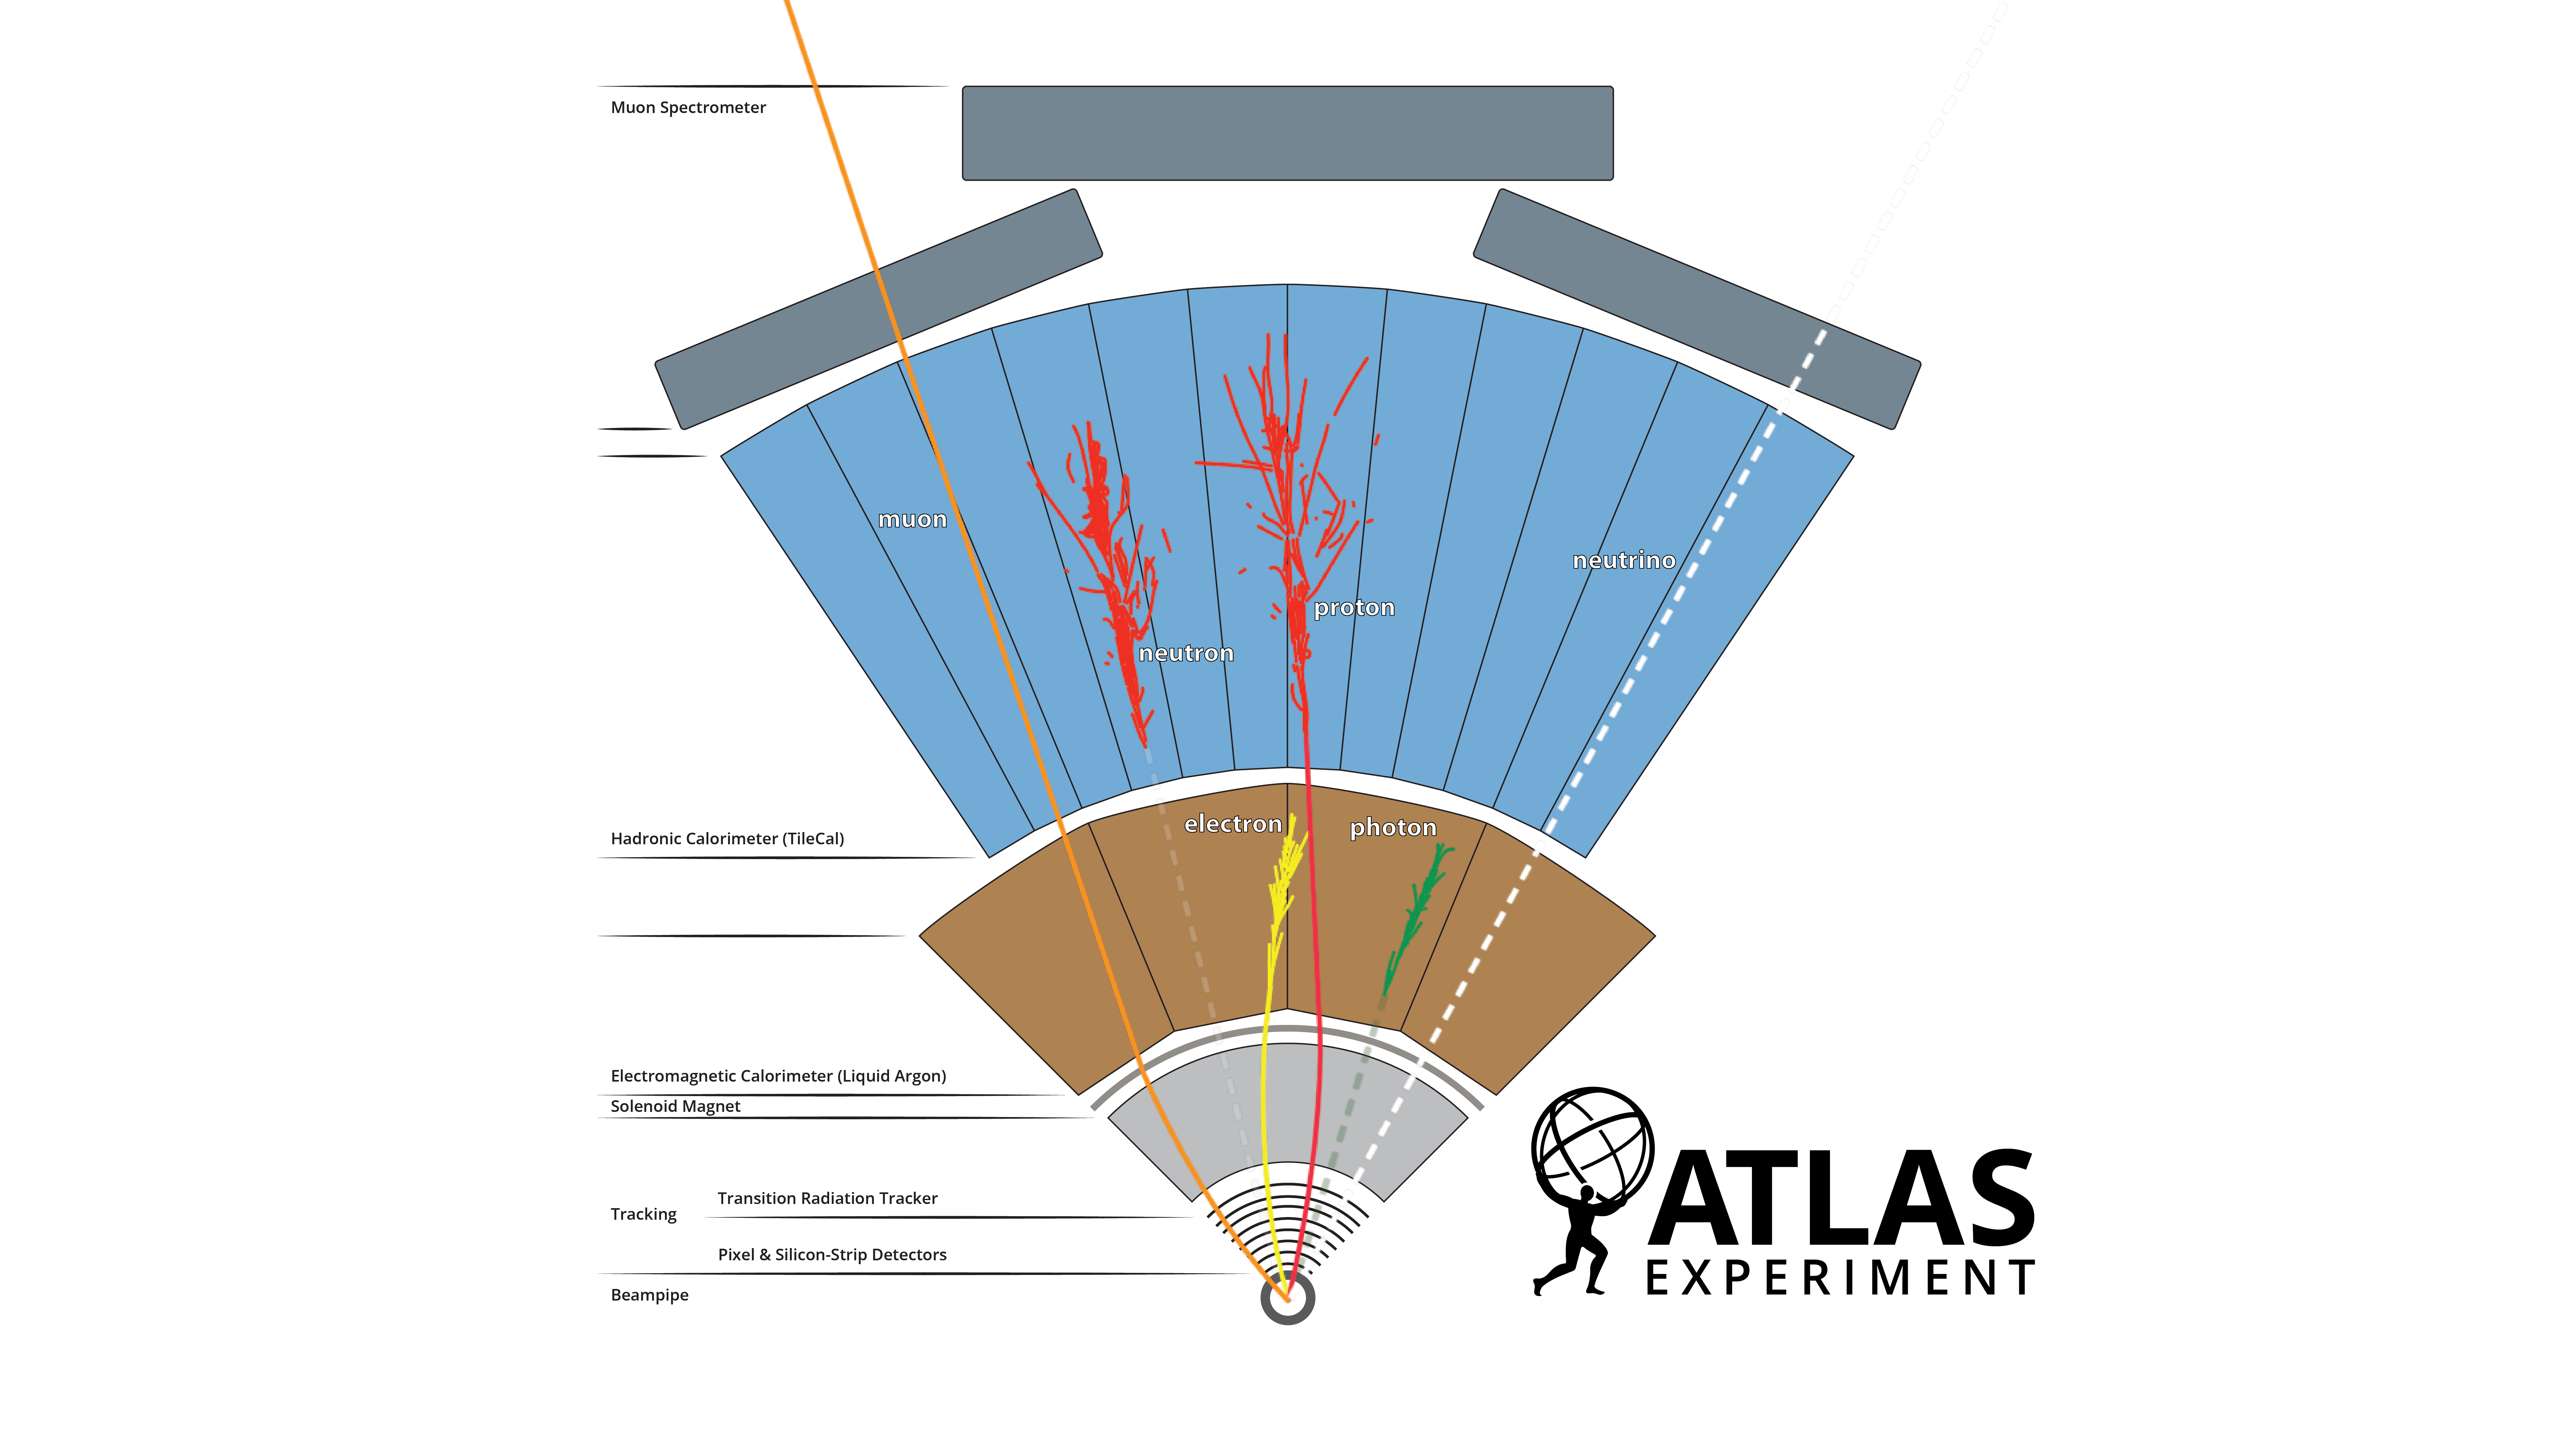
\includegraphics[width=1.0\textwidth]{images/atlas_particles.png}
  \caption{Schematic representation in the $x-y$ plane of fundamental particles interacting with the different ATLAS sub-systems~\cite{Bianchi:2837191}}
  \label{fig:reco}
 \end{figure}

\section{Tracks, vertices and energy clusters}
\label{sec:tracks}

As mentioned before, tracks, vertices and calorimeter energy clusters, as well as matching requirements among themselves, are the essential inputs to the reconstruction and identification of physics objects which are going to be discussed in this chapter

The first step in the reconstruction of an event is the identification of the trajectories defined by charged particles in the ID, which are called tracks.
Charged particles traversing the ID leave spatially precise hits in the Pixel and SCT layers. Under the solenoidal 2~T magnetic field, their paths bend into helices, with curvature inversely related to transverse momentum. 
Each reconstructed track is described by five parameters: transverse momentum \(p_T\), polar angle \(\theta\), azimuth angle \(\phi\), the impact parameter in the transverse plane with respect to the interation point \(d_0\), and longitudinal impact parameter, in the longitudinal plane \(z_0\). Figure~\ref{fig:tracks} shows a representation of those parameters.

\begin{figure}[htbp]
  \centering
  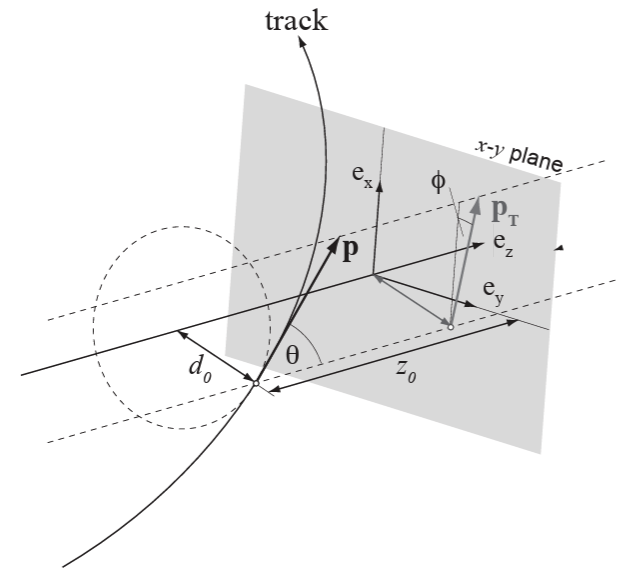
\includegraphics[width=0.6\textwidth]{images/tracks.png}
  \caption{Schematic representation in the $x-y$ plane of fundamental particles interacting with the different ATLAS sub-systems~\cite{Bianchi:2837191}}
  \label{fig:tracks}
 \end{figure}

The reconstruction proceeds in several stages~\cite{tracks}. First, nearby hits or sensor measurements above a threshold are clustered and triplets of clusters form track seeds. Next, a combinatorial Kalman filter~\cite{kalman} extends each seed outward, adding compatible clusters layer by layer and updating the track parameters at each step (i.e. the momentum or its position). Multiple overlapping candidates are pruned by an ambiguity solver, which scores each track using fit \(\chi^2\), \(p_T\), the number of associated clusters, and the count of “holes” (expected but missing hits), to favor well–measured and high-\(p_T\) trajectories.

Finally, surviving candidates undergo a global fit, incorporating all valid clusters to refine the five helicoidal parameters. The chosen tracks are required to have at least 7 clusters between the Pixel and the SCT detectors, less than 2 holes in the Pixel and a maximum of 2 holes in the SCT sub-detector, a $p_{T} > 500$~MeV and a $|\eta|>2.5$. In addition, the track is required to satisfy $|d0|<2$~mm and $|z0\sin\theta|<3$~mm, and then it is reatined for downstream object reconstruction.

Subsequently, the tracks are used to reconstruct vertices, which correspond to the locations where particle interactions occur. Vertices are identified by extrapolating tracks backward to their point of closest approach. We are primarily interested in those vertices occurring near the proton–proton interaction region. The primary vertex of an event is defined as the interaction point where the colliding protons met, while all other reconstructed vertices are treated as pile-up or secondary vertices, which are also crucial for 
b-tagging and identifying other displaced objects. For a detailed description of primary-vertex reconstruction in ATLAS see refs.~\cite{vertex_run1,vertex_run2,vertex_run3}.

Generally, vertex reconstruction proceeds in two phases: finding and fitting. First, vertex finding groups tracks into vertex candidates. An initial seed position is chosen, and then an iterative fit adjusts both the vertex position and individual track weights, which quantify how well a track originates from that vertex. Tracks whose weights fall below a threshold at the final iteration are excluded and reserved for forming additional vertices. This cycle repeats on the remaining unassigned tracks until no further vertices emerge. 
Next, vertex fitting refines the 3D location of each candidate using its assigned tracks. The event’s primary vertex is defined here as the one whose tracks have the largest $\sum p^2_{T}$, although alternative primary-vertex definitions exist.

The missing ingredient was the energy clusters. Particles leave energy deposits in individual cells of ATLAS calorimeters, which are clustered together forming 3D topological cell clusters, called topo-clusters~\cite{topo}.

Topo-clusters are constructed by first identifying seed cells whose measured signal exceeds the expected electronics noise by a significant amount. From each seed, adjacent cells are added iteratively whenever their signal-to-noise ratio passes a predefined threshold, and this expansion ceases once no further cells meet the criterion. Cells with low significance are excluded, naturally filtering out noise. Because hadronic showers spread more broadly than electromagnetic ones, a single topo-cluster may capture an entire shower, only part of it, or even combine energy deposits from multiple particles. 

Since the ATLAS calorimeters are non-compensating, which means that their response to hadrons is lower than to electrons or photons of the same energy, all signals are initially recorded on the electromagnetic energy scale. To account for the differing responses and energy losses in inactive materials, topo-clusters undergo dedicated calibrations. After calibration, each cluster can be treated as a massless pseudo-particle, described uniquely by its calibrated energy and position in the $\eta - \phi$ space.

\section{Muons}
\label{sec:muons}

Muons are reconstructed and identified using combined information from the Inner Detector (ID) and the Muon Spectrometer (MS). These minimum-ionizing particles with long penetration length through the calorimeters leave very small energy deposits in the subdetectors.
\subsection*{Reconstruction} 
Track candidates are first found independently in the ID and in the MS. In the ID, the tracks are reconstructed exactly as explained in Section~\ref{sec:tracks}.

In the Muon System, track fragments are formed by combining hits that lie close together along the expected trajectory of a muon and that are consistent with having originated from the proton–proton collision interaction point (i.e., they point back to the IP)~\cite{muon_reco_run2}. 
In order to create seeds, segments from the middle station of the MS are first used, and these seeds are then extended into the inner and outer detector layers. A track candidate requires at least two such segments, and a given segment may contribute to multiple candidates. Ambiguities are resolved and the candidate is accepted or rejected by performing a $\chi^2$-fit to the hits associated with each track candidate, together with additional track quality requirements.

Once we have both trajectories reconstructed in ID and MS, various muon reconstruction categories are defined based on the detector information they exploit. “Combined” muons result from a joint fit of Inner Detector and Muon Spectrometer tracks, typically using an outside-in strategy that projects MS tracks back into the ID; an inside-out approach, seeding from the ID and extending into the MS, is also employed. “Extrapolated” muons rely uniquely on MS tracks extrapolated to the beamline, ensuring compatibility with the primary vertex, and extend coverage into the forward region $2.5 \lt |\eta| \gt 2.7$
beyond the ID acceptance. “Segment-tagged” muons begin with an ID track that is matched to at least one precision chamber segment in the MS, recovering muons that traverse only a single spectrometer layer. Finally, “calorimeter-tagged” muons are identified by isolated, minimum-ionizing energy deposits in the calorimeter aligned with an ID track, filling in gaps where MS coverage is incomplete.

\subsection*{Identification} 

On top of Reconstruction, the muon identification in ATLAS applies additional selection criteria to the reconstructed muons in order to reduce contribution from most likely background sources like charged hadron decays, in-flight decays...
Seeking for a balance between identification efficiency and background rejection, different working points are defined encapsulationg these selection requirements. The main ones are Loose, Medium and Tight working points, plus two additional ones devoted to low-$p_{T}$ and high-$p_{T}$ target muons.

The Loose WP accepts all reconstructed muon types (Combined, Inside–Out, Segment‐Tagged, and Calorimeter‐Tagged) with minimal kinematic cuts (e.g.\ $p_T>4,$GeV), achieving maximal efficiency at the cost of higher fake rates, particularly in the reduced‐coverage region $|\eta|<0.1$. The Medium WP restricts to Combined and Inside–Out muons within $|\eta|<2.47$, requires at least three precision‐chamber hits spanning two muon‐spectrometer layers (one layer suffices for $|\eta|<0.1$), and imposes a compatibility cut on the charge‐over‐momentum difference between the Inner Detector and Muon Spectrometer measurements of less than seven standard deviations. Finally, the Tight WP further tightens these requirements by demanding a three‐hit segment in two distinct spectrometer stations and stronger cuts on the $q/p$ significance and inter‐subdetector momentum consistency, all optimized in $(p_T,\eta)$ bins to suppress residual backgrounds.

In simulated \ttbar and $Z\to\mu\mu$ samples, the Medium WP achieves prompt‐muon efficiencies up to 97$\%$~\cite{muon_reco_run2}, while retaining background muons (e.g.\ from hadron decays) at the per‐mille level. Discrepancies between data and simulation are corrected via $\eta$–$\phi$–binned scale factors—typically within a few percent of unity—to account for local detector non‐uniformities such as support‐structure regions.

\subsection*{Isolation} 

Since prompt muons are typically produced well isolated from other activity, muon isolation is applied to reject non-prompt candidates. Here, isolation quantifies additional detector activity around the muon, while the decay of high-momentum objects, whose products are often collimated, including muons, can naturally appear isolated.
Two isolation variables are used. Track-based isolation is defined as the scalar sum of the transverse momenta of all tracks with $p_{T}\gt1$~GeV within a cone around the muon (excluding the muon itself), where the cone size shrinks with increasing muon momentum, $p^{\mu}_{T}$, as $\Delta R = \text{min}(0.3, 10 \text{GeV}/p^{\mu}_{T})$.
Calorimeter-based isolation is computed by summing the energy deposits of topo-clusters within a fixed cone of $\Delta R=0.3$ around the muon (again excluding the muon’s own deposit) and applying pile-up corrections. Each isolation criterion is then expressed as a ratio of the isolation sum to the muon’s transverse momentum.
Several working points are defined: Loose, Gradient, and FCTight (“fixed‐cut tight”) all use both track‐ and calorimeter‐based isolation; FCTO (“fixed‐cut track‐only”) applies only the track‐based requirement.

\section{Jets and flavour tagging}
\label{sec:jets}
As explained in Section~\ref{subsec:proton}, in the proton-proton collisions the quarks and gluons produced at the partonic level undergo hadronisation, resulted in collimated jets measured by the ATLAS detector via the tracks registered in the ID and energy deposits in the calorimeter system. 

Jet reconstruction in ATLAS is fundamentally based on sequential recombination algorithms, the most widely used being the \antikt algorithm~\cite{Cacciari_2008}. This algorithm is designed to be stable in the presence of soft and collinear emissions from partons, operating by defining a distance measure between any two objects $i$ and $j$ (which may be tracks or topo-clusters) as follows:
\begin{equation}
  d_{i,j} = \text{min}(p^{2p}_{T,i},p^{2p}_{T,j})\frac{\Delta^{2}_{ij},R^{2}},
\end{equation}
being $\Delta^{2}_{ij} = (\eta_{i} - \eta_{j})^2 + (\phi_{i} - \phi_{j})^2$ the distance in the $\eta$-$\phi$ plane and $R$ the radial parameter that defines the jet size. Setting the exponent $p$ to −1 ensures that objects with higher transverse momenta dominate the clustering procedure. The beam distance is also computed for each object as:
\begin{equation}
  d_{iB} = p^{2p}_{T,i},
\end{equation}
so the smaller of the two distance measures is chosen at each iteration. If \(d_{ij}\) is smaller, objects \(i\) and \(j\) are merged into a new object. If \(d_{iB}\) is smaller, then object \(i\) is identified as a jet and removed from the list of objects to process, and the procedure continues until no objects remain. The parameter \(R\) sets the jet radius and the extent of the \(\eta\)–\(\phi\) space used for clustering. It typically takes values of \(R = 0.4\) for small-radius jets or \(R = 1.0\) for large-radius ones~\cite{jets_cluster}.

Once jets are reconstructed, several energy calibrations are applied in order to correct detector effects y conseguir un matching accurate con la energía del jet at particle-level~\cite{jets_calib}. The first stage of jet calibration addresses pile-up effects arising from additional proton–proton interactions. An event-by-event correction is computed using the jet area and the transverse momentum density of the event, followed by residual corrections that depend on the number of reconstructed primary vertices and the average pile-up multiplicity. 

Next, the Jet Energy Scale (JES) calibration adjusts each jet’s reconstructed energy and pseudorapidity so that, on average, it matches the true particle-level jet energy. This is achieved via $p_{T}$- and $\eta$-dependent scale factors derived from full detector simulation, accounting for the differing calorimetric response to electromagnetic versus hadronic showers. After JES, a Global Sequential Calibration (GSC) applies multiplicative corrections based on the jet’s internal properties, such as width, track–vertex association, and flavor-sensitive observables, in order to reduce residual biases between quark- and gluon-initiated jets and to compensate for variations in fragmentation.

An in-situ calibration then removes any remaining mismodeling by comparing the balance between jets and well-measured reference objects (like isolated photons) in data; these data-driven correction factors, supplemented by multijet balance methods, are applied only to data jets to align their response with simulation. The Jet Energy Resolution (JER)~\cite{Aaboud_2017} is subsequently measured using dijet balance and random-cone techniques, yielding a $p_{T}$- and $\eta$-dependent resolution function. Simulation jets are smeared to reproduce the observed resolution in data.

Finally, to suppress pile-up jets, the Jet Vertex Tagger (JVT)~\cite{ATL-PHYS-PUB-2014-001} exploits track-based variables, particularly the fraction of jet tracks originating from the primary vertex, together with event-level pile-up information, to discriminate hard-scatter jets within $|\eta|<2.4$. For the forward region $(2.4<|\eta|<<4.5)$, the forward JVT (fJVT) extends this technique, ensuring consistent pile-up rejection across the full calorimeter acceptance. 

\subsection*{$b$-jets tagging} 

Identifying jets originating from $b$-quarks ($b$-jets)is vital for many LHC analyses, especially those involving top quarks or Higgs bosons. $b$-hadrons travel a few millimeters before decaying, creating displaced secondary (and sometimes tertiary) vertices and tracks with large impact parameters relative to the primary collision point.
Simple b-taggers, like IP2D and IP3D, exploit these features by measuring the significance of transverse and longitudinal impact parameters and creating discriminants that recognizes tracks associated to non-primary vertex~\cite{btag_1,btag_2}, while secondary-vertex algorithms reconstruct displaced vertices and use features like invariant mass of tracks associated to the secondary vertex, vertex flight distance, and track multiplicity to distinguish $b$-jets from light-flavor or gluon jets.

Modern high-level $b$-taggers combine these low-level discriminants via machine-learning techniques in order to improve the overall performance, also being able to tag intermediate $c$-hadrons and involved tertiary vertices. The DL1r algorithm, used for the first round of Run-2 data~\cite{tagging}, for example, feeds IP2D, IP3D, and secondary-vertex outputs into a deep neural network, along with additional variables, such as those from a jet-vertex finder, for improved $c$-jet rejection and an RNN to capture track correlations. DL1r produces three scores, corresponding to the probabilities that a jet originates from a $b$-, $c$-, or light quark, achieving superior separation compared to individual taggers.

The performance of $b$-tagging algorithms is characterized by the efficiency to identify $b$-jets and the rejection factors achieved against $c$-jets and light-flavor jets.  Standard working points are defined at approximately 60\%, 70\%, 77\%, and 85\% $b$-jet efficiency, trading off signal efficiency against background suppression.  To correct for residual differences between simulation and data, per-jet scale factors are measured in control regions with well-known flavor content (e.g.\ $t\bar t$ events) and applied to all Monte Carlo samples so that the simulated tagging efficiencies reproduce those observed in collision data.

For Run-3 and R.22 Run-2 data processings, the ATLAS b-tagging algorithm has evolved from the DL1r-based DNN to the enhanced GN2 network~\cite{new_tagging}, which integrates Graph Neural Network techniques to better capture the relational information among tracks and secondary vertices. GN2 demonstrates improved separation power between \(b\), \(c\), and light-flavour jets, particularly at high pile-up, yielding a ~10\% gain in light-jet rejection at the 70\% \(b\)-jet efficiency WP compared to DL1r.  


\section{Hadronic tau-leptons}
\label{sec:tauhad}
Electrons and muons, usually referred to as light leptons, interact with the detector material and leave clear signatures. In contrast, \(\tau\)-leptons, due to their greater mass, decay rapidly after approximately \(1\ \mu\mathrm{m}\), without reaching any detector layer. Therefore, they are typically reconstructed and identified from their decay products. \(\tau\)-leptons can decay leptonically, to electrons or muons plus neutrinos (manifesting as missing transverse energy, \(E_{\mathrm{T}}^{\mathrm{miss}}\)), so no specialized reconstruction is performed in those cases. 
In fact, a key feature distinguishing these leptons from prompt leptons produced directly in the hard scattering is that the \(\tau\)-decay vertex is slightly displaced from the \(pp\) primary vertex, due to the finite lifetime of the \(\tau\), resulting in an impact-parameter distribution for the final-state leptons that differs from that of prompt leptons. 
On the other hand, for hadronically decaying \(\tau\)-leptons (\(\tau_{\text{had-vis}}\) from now on), which account for a total branching ratio of 65\%, a dedicated reconstruction and identification procedure exists, since these decays yield jets composed primarily of charged and neutral pions~\cite{ParticleDataGroup}.

The reconstruction of \(\tau_{\text{had-vis}}\) candidates begins with jets as seeds, clustered using the anti-\(k_{t}\) algorithm with a radius parameter \(R = 0.4\).  Candidates are required to satisfy \(p_{T} > 10\ \mathrm{GeV}\) and \(|\eta| < 2.5\).  The \(\tau\)-lepton energy is initially estimated by summing the energies of topo-clusters within a cone of \(\Delta R = 0.2\) around the seed jet axis.  Within the same cone, the transverse momenta of all associated tracks are summed to reconstruct the \(\tau\)-decay vertex.  
The vertex with the highest summed \(p_{T}\) is chosen, and only tracks with \(p_{T} > 1\ \mathrm{GeV}\), at least two pixel hits, and at least seven hits in the SCT and TRT are retained.  Impact-parameter requirements relative to the \(\tau\)-vertex are \(|d_{0}| < 1.0\ \mathrm{mm}\) and \(|z_{0}\sin\theta| < 1.5\ \mathrm{mm}.\)
The \(n\)-prong \(\tau_{\text{had-vis}}\) decay can consist of \(n\) charged hadrons (mostly pions, occasionally kaons), so candidates are categorized as 1-prong or 3-prong.  In the first Run-2 production, a dedicated Boosted Decision Tree (BDT) was trained to classify these track patterns; for the R.22 Run-2 and Run-3 samples, this was replaced by a Recurrent Neural Network (RNN) for \(\tau\)-track classification~\cite{ATL-PHYS-PUB-2022-044}.  

After reconstructing the \(\tau_{\text{had-vis}}\) candidate, distinguishing it from quark- and gluon-initiated jets that can mimic its signature is achieved using separate RNNs for 1-prong and 3-prong \(\tau_{\text{had-vis}}\) decays.  These networks are trained to be robust across the full \(p_{T}\) spectrum of the \(\tau_{\text{had-vis}}\) and under varying pile-up conditions, exploiting features of the \(\tau\)-lepton—namely its weak decay, which produces narrower jets with lower track multiplicities than QCD jets.  
The RNN output defines four working points (Tight, Medium, Loose, VeryLoose), with 1-prong efficiencies of 60\%, 75\%, 85\% and 95\%, and 3-prong efficiencies of 45\%, 60\%, 75\% and 95\%, respectively, balancing signal retention against background rejection.  For the R.22 Run-2 and Run-3 samples, this RNN has been superseded by a Graph Neural Network (similar to that used for \(b\)-tagging~\cite{new_tagging}), yielding significantly improved fake-\(\tau_{\text{had-vis}}\) rejection and reducing this background by up to 40\% in our analysis.  

Finally, during the first Run-2 production, an additional BDT, known as the electron-veto BDT (eBDT), was trained to reject background from electrons that can mimic 1-prong \(\tau_{\text{had-vis}}\) decays.  The eBDT uses high-level inputs such as calorimeter cell deposits and track features, with TRT information playing a crucial role in distinguishing electrons from hadrons.  It achieved over 95\% efficiency for genuine \(\tau_{\text{had-vis}}\).  For the R.22 Run-2 and Run-3 datasets, this task is now performed by a dedicated RNN~\cite{ATL-PHYS-PUB-2022-044}.

\section{Missing transverse momentum}
\label{sec:met}

Energy–momentum conservation guarantees that the total four–momentum of the initial state equals that of the final state.  In \(pp\) collisions, the longitudinal momentum cannot be determined because the colliding partons carry unknown fractions of the proton momentum.  However, since the incident protons travel and collide along the longitudinal axis, the total momentum in the transverse plane must be zero.  

Thus, the missing transverse momentum (\et) quantifies the transverse energy carried away by invisible particles in the collision, as seen by the ATLAS detector.  These invisible particles may be neutrinos or other weakly interacting species such as dark matter candidates.  It is computed as the negative vector sum of all reconstructed and calibrated objects in ATLAS:

\begin{equation}
    \et = \underbrace{- \sum_{\text{electrons}} p_{\text{T}}^{e} + \sum_{\text{muons}} p_{\text{T}}^{\mu} + \sum_{\text{photons}} p_{\text{T}}^{\gamma} + \sum_{\text{taus}} p_{\text{T}}^{\tau} + \sum_{\text{jets}} p_{\text{T}}^{j}}_{\text{hard term}} \underbrace{- \sum_{\text{unused tracks}} p_{\text{T}}^{\text{tracks}}}_{\text{soft term}},
\end{equation}\noindent

The missing transverse momentum has two contributions: the hard term, made up of calibrated electrons, photons, hadronically decaying \(\tau\)-leptons, jets, and muons, and the soft term, which comprises energy not clustered into these objects. In ATLAS, the soft term is typically formed from tracks associated with the primary vertex, making it less sensitive to pile-up.

In simulations, the performance of \et is validated by comparing MC and data in processes such as \(Z\to\mu^{+}\mu^{-}+\text{jets}\), where the true \et is near zero.  Discrepancies can expose detector effects, jet miscalibration, or residual pile-up.  

    
%-------------------------------------------------------------------------------

%-------------------------------------------------------------------------------
\chapter{Machine Learning Techniques}
\label{chap:machine_learning}




Machine learning (ML) algorithms, often referred to as multivariate (MVA) techniques, play a central role in classification tasks where efficient signal-to-background separation is required. Their increasing relevance in particle physics arises from their ability to model complex correlations among observables, providing substantial improvements in both classification and analysis optimisation. 

This chapter introduces the concepts of supervised learning and focuses on the two algorithms used throughout this thesis: deep neural networks (DNNs) and boosted decision trees (BDTs). Both methods have demonstrated excellent performance in a wide range of applications, and their implementation in the analyses presented here follows closely the principles outlined in Ref.~\cite{Goodfellow-et-al-2016}.

In general terms, a ML algorithm can be defined as one that is capable of learning to perform a specific task based on input data, which typically consists of a multidimensional set of features. This thesis focuses specifically on supervised machine learning algorithms, which are trained using a set of $n$ input data elements, $X = \left\{\vec{x_{0}}, \vec{x_{1}}, ..., \vec{x_{n}} \right\}$, where each element encapsulates $m$ features, as previously mentioned, $\vec{x_{i}}=(x_{i,0}, x_{i,1}, ..., x_{i,m})$. The term ``supervised'' is used because each data point is associated with a known true label $y_{i}$, and the goal is to infer this label for new, unseen data using the input provided during the algorithm training.

\subsubsection*{Dataset preparation}
When training a supervised ML model, the so-called training dataset is used to optimize the model parameters. However, in order to properly evaluate the model's performance and select its best version, one must rely on data that has not been seen during the training process. Otherwise, the model could learn overly specific features or fluctuations from this subset that are not present in real experimental data. This would ultimately lead to degraded performance when applied to unseen data. This issue is known as overtraining or overfitting.

To mitigate this problem and improve generalization, it is common to introduce an additional validation dataset. The model's performance is monitored on this separate dataset during training in order to guide the optimization process and prevent overfitting. When used, the version of the model that achieves the best performance on the validation data is typically selected as the final one.

For a final, unbiased evaluation of the model’s performance, a third dataset, called test dataset, is employed. Since both the training and validation datasets have already influenced the model, they cannot be used to assess its final quality. Typically, the three datasets (training, validation, and test) are obtained from the same original input sample by randomly splitting its data points.

Another widely used approach to maximize the use of available data is the \textit{k-fold} cross-validation technique~\cite{tmvatoolkit}. In this method, the original dataset is split into $k$ equal parts (or ``folds''). The model is then trained $k$ times, each time using $k-1$ folds for training and the remaining one for validation. This allows every data point to be used for both training and validation at different stages, providing a more robust performance estimate and making efficient use of limited datasets. A diagram illustrating the definition of these folds can be found in Figure~\ref{fig:kfold}.
\begin{figure}[htbp]
    \centering
    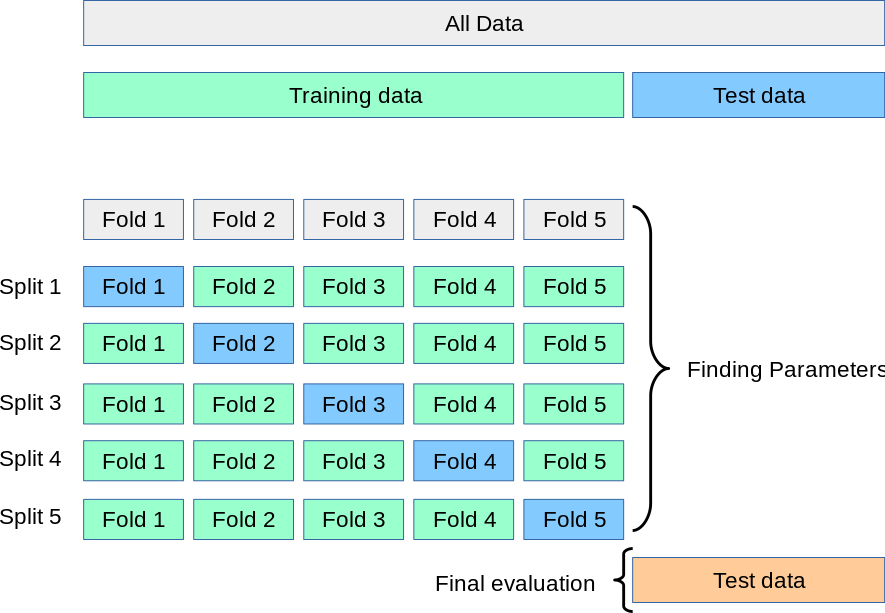
\includegraphics[width=0.6\textwidth]{kvalidation.png}
    \caption{Schematic illustration of the $k$-fold splitting procedure used for training and testing~\cite{scikit_learn_cv}.}
    \label{fig:kfold}
\end{figure}

\subsubsection*{Type of prediction}
A ML algorithm can be designed to perform various tasks, even multiple ones simultaneously. These include data synthesis and sampling, anomaly detection, and others. Many of these tasks are also employed in the context of high energy particle physics.
In this thesis, the focus is specifically placed on classification, the most fundamental task besides regression.

Classification problems generally involve that the learning algorithm is asked to determine which of $C$ predefined categories a given input belongs to. Formally, this is often expressed as finding a function $f: \mathbb{R}^n \rightarrow \{1, \dots, C\}$, where a vector of input features $\vec{x}$ is assigned a class label $y = f(\vec{x})$. In many practical implementations, especially in physics applications, the model does not directly return a class label, but instead provides a probability distribution over all possible classes. The final classification decision can then be made by selecting the class with the highest predicted probability.

If $C = 2$, the task is referred to as binary classification, and the model typically outputs a single value representing the probability that the input belongs to one of the two classes (e.g., signal vs background in our domain). The probability of the alternative class is simply $1 - f(\vec{x})$. If $C > 2$, the task is referred to as multinomial classification and in such cases, one probability is returned for each class and the outputs can be combined into a single discriminant using a likelihood ratio as prescribed by the Neyman-Pearson lemma~\cite{Neyman:1933wgr}:
\begin{equation}
    L = \frac{p_0}{\sum_{i=1}^C f_i p_i},
\end{equation}
where $p_i$ is the predicted probability for class $i$ and $f_i$ is a configurable weight that adjusts the importance of each class in the denominator. By tuning the $f_i$, the classifier’s sensitivity to specific categories can be adjusted to fit the needs of a particular analysis.

\subsubsection*{Loss function}

To quantify the optimization of a supervised machine learning model during its training, it is necessary to measure how well it is performing. For this purpose, a loss (or cost) function is defined, which is the function to be minimized during the training of the model.  
The loss function ($\mathcal{L}$) of a dataset is computed by evaluating the loss value on each data point and averaging over all points:
\begin{equation}
    \mathcal{L}(\hat{\vec{y}},\vec{y}) = \frac{1}{N}\sum^{N}_{i=1} \mathcal{L}(\hat{y}_{i},y_{i}),
\end{equation}
where the $\hat{\vec{y}}$ are the set of predictions made by our model, and ${\vec{y}}$ are the corresponding true labels, $N$ is the number of data points in our dataset. The choice of the loss function is determined by the problem under consideration, leading to more or less efficient solutions.
In the context of regression problems, the simplest one, like a linear fit of a straight line, the Mean Absolute Error (MAE) is commonly used, $\mathcal{L}(\hat{y},y) = |\hat{y} - y|$.
For binary classification, the most commonly used loss function is the so-called binary cross-entropy, $\mathcal{L}(\hat{y},y) = -y\ln(\hat{y}) + (1-y)\ln(1-\hat{y})$.
Its generalization to the case of multinomial classification is obtained through the categorical cross-entropy, defined as:
\begin{equation}
    \mathcal{L}(\hat{y},y) = - \sum_{C} y_{c}\ln(\hat{y}_{c}),
\end{equation}
being $c$ each of the classes considered in the problem.
\subsubsection*{Performance measurements}
As mentioned earlier, the final performance of the trained model must be tested on a totally unseen test dataset. The loss function primarily serves to guide the optimization process during training, although a low final value often indicates the goodness of our model. Specific metrics or figures of merit, depending on the problem at hand, are usually employed to gain a deeper understanding of the efficiency of our ML models.

In the case of classification problems, as in the work presented in this thesis, the most commonly used figure of merit is the Receiver Operating Characteristic (ROC) curve, which provides a clear visualisation of the performance of a binary classifier in terms of signal and background identification efficiency, which is precisely the core issue to address.

The goal is to optimise both quantities, and to obtain the ROC curve computed for different values of the discriminant output of the algorithm. The signal identification efficiency is calculated as the number of candidates with a discriminant value above the threshold, divided by the total number of signal candidates. Instead of background efficiency, its inverse is typically used: the background rejection. Plotting background rejection against signal efficiency allows the identification of the model that offers the best performance, as illustrated in the example in Figure~\ref{fig:roc_curves}. The optimal model will be the one that reaches values closest to the upper right corner.

\begin{figure}[htbp]
    \centering
    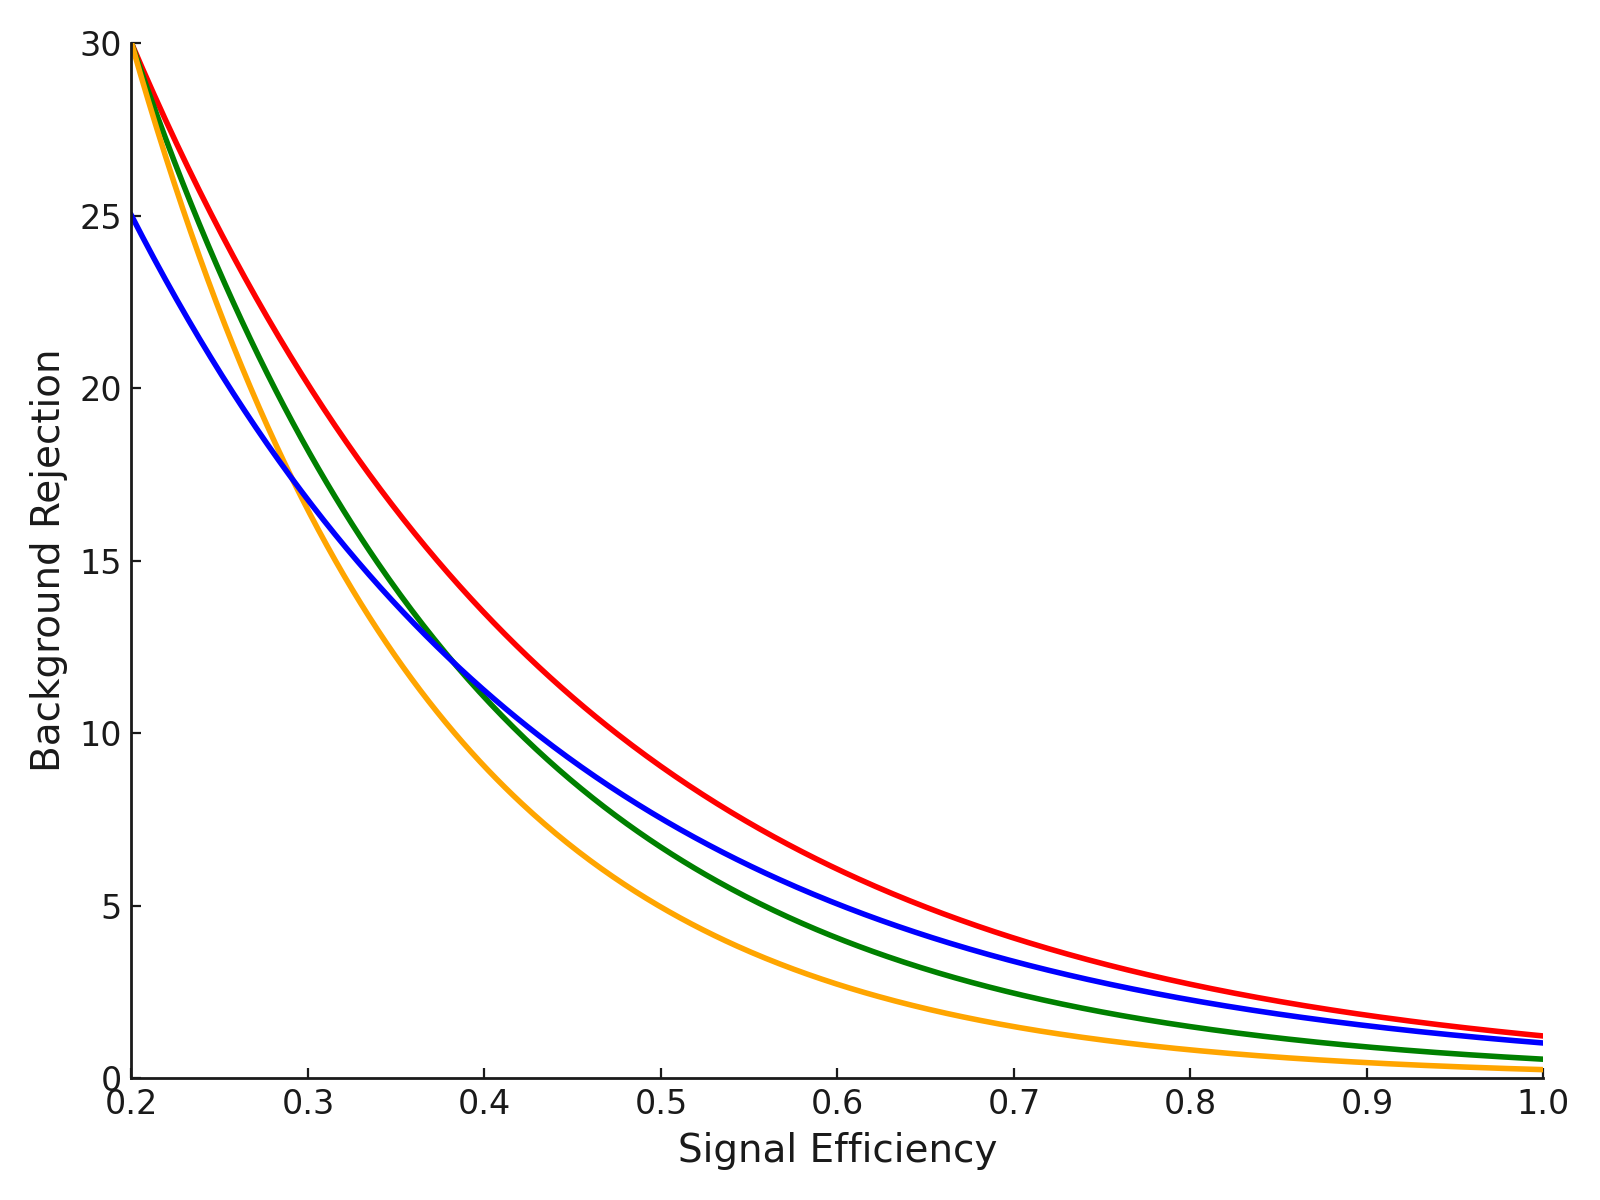
\includegraphics[width=0.7\textwidth]{images/roc_curves_clean.png}
    \caption{Example of ROC curves evaluated for different models in terms of signal efficiency and background rejection.}
    \label{fig:roc_curves}
  \end{figure}

\section{Deep Neural Networks}
\label{sec:dnn_general}
% Esta sección contendrá los fundamentos de las DNN: arquitectura, función de activación,
% función de pérdida, entrenamiento, regularización, overfitting, etc.
% Será genérica y no específica de electron ID, para poder referenciarla desde otras secciones.

One of the most widely used and well-known ML algorithms is Neural Networks (NNs). A broad variety of architectures exists, but the most basic ones are the Deep Neural Networks (DNNs), generally referring to any NN with multiple hidden layers. In this thesis, reference is implicitly made to Feed-Forward DNNs, where information flows in one direction, from input to output, without any feedback or recurrence.

In general terms, the simplest form of a NN is a linear layer, which applies an affine transformation to the input data and can be described as:
\begin{equation}
    \vec{x}_{out} = W\vec{x}_{in} + b,
\end{equation}
where $W$ is a weight matrix associated with each node, $b$ is a bias vector, and $\vec{x}_{\text{in}}$ and $\vec{x}_{\text{out}}$ are the input and output feature vectors. Both the weights and the biases are parameters learned and optimized by the NN during training.

In the end, to build a DNN, depending on the complexity of the problem, the architecture is constructed by stacking multiple layers, which are applied sequentially, as illustrated in Figure~\ref{fig:dnn}.
\begin{figure}[htbp]
    \centering
    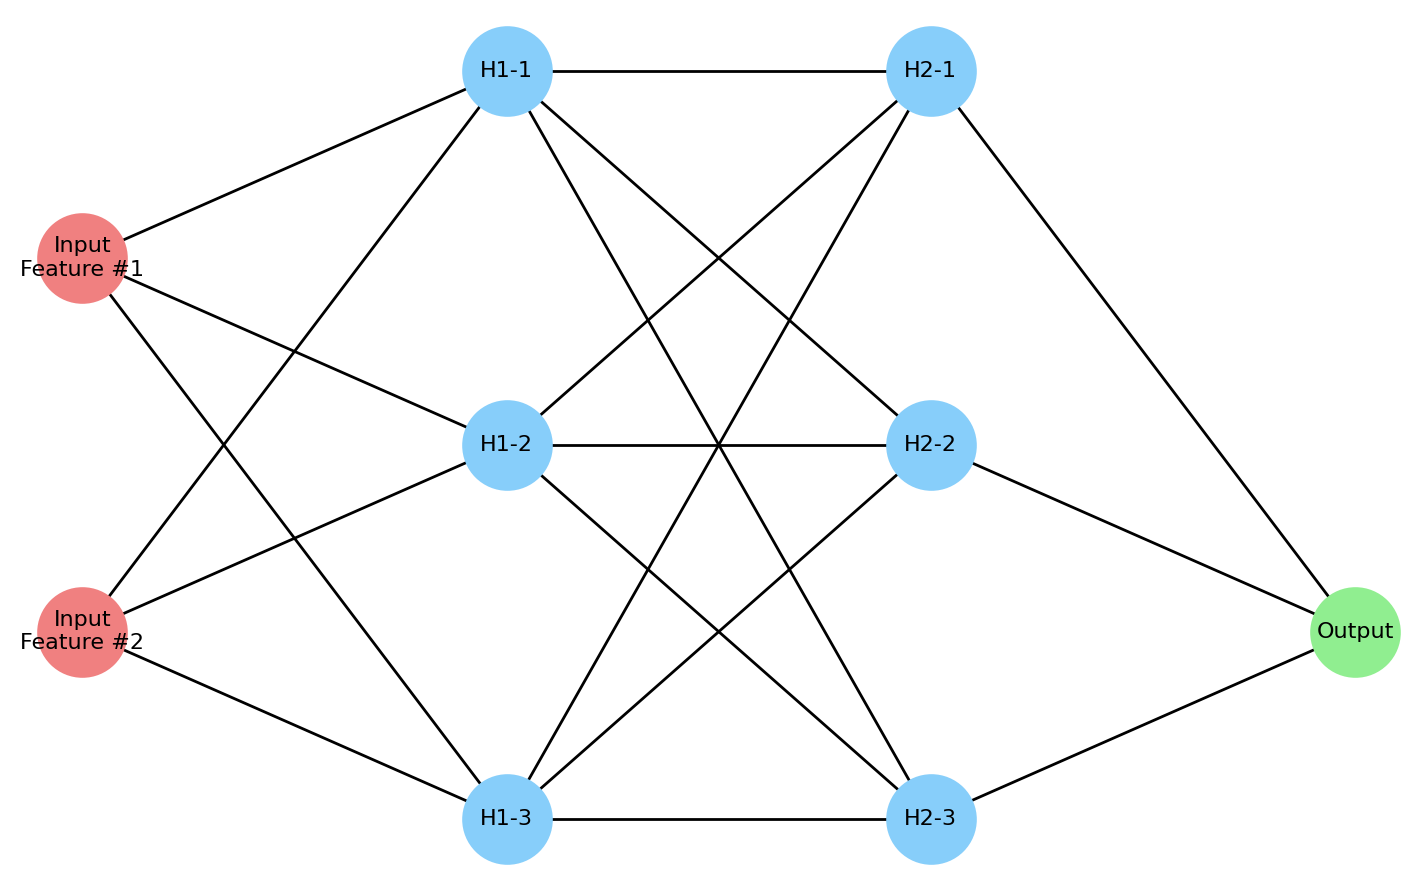
\includegraphics[width=0.7\textwidth]{images/dnn.png}
    \caption{Diagram of Neural Network architecture with two input features, two hidden layers with three nodes each and one output.}
    \label{fig:dnn}
  \end{figure}

It is important to note that the real dependencies and correlations among the input features are very likely to be non-linear and follow more complex patterns. However, since a single layer applies an affine transformation, the output will ultimately remain affine.
To enable the algorithm to learn and handle non-linearities, activation functions are used.

\subsection{Activation functions}
The non-linear behaviour of a NN is achieved by passing the output of a linear layer through an activation function. One of the most commonly used activation functions is the Rectified Linear Unit (ReLU), which is simply defined as follows
\begin{equation}
    f(x)= \left\{\begin{array}{lcc} x, & if & x \ge 0 \\ 0 & if & x < 0 \\ \end{array}\right}.
\end{equation}

This simple action of setting the unit for positive inputs and zeroing the function otherwise introduces a non-linearity, and its derivative is straightforward to compute, which is beneficial for optimization.  

There are other options that, in certain cases, can improve the performance of the NN output, such as the Leaky Rectified Linear Unit (Leaky ReLU), which modifies the negative part to have a small slope~\cite{Maas2013RectifierNI}, meaning that negative values are not discarded but scaled by a certain factor. Another example is the Gaussian Error Linear Unit (GELU)~\cite{hendrycks2023gaussianerrorlinearunits}. As an illustration, a representation of these activation functions and their derivatives is shown in Figure~\ref{fig:activation}.
\begin{figure}[htbp]
    \centering
    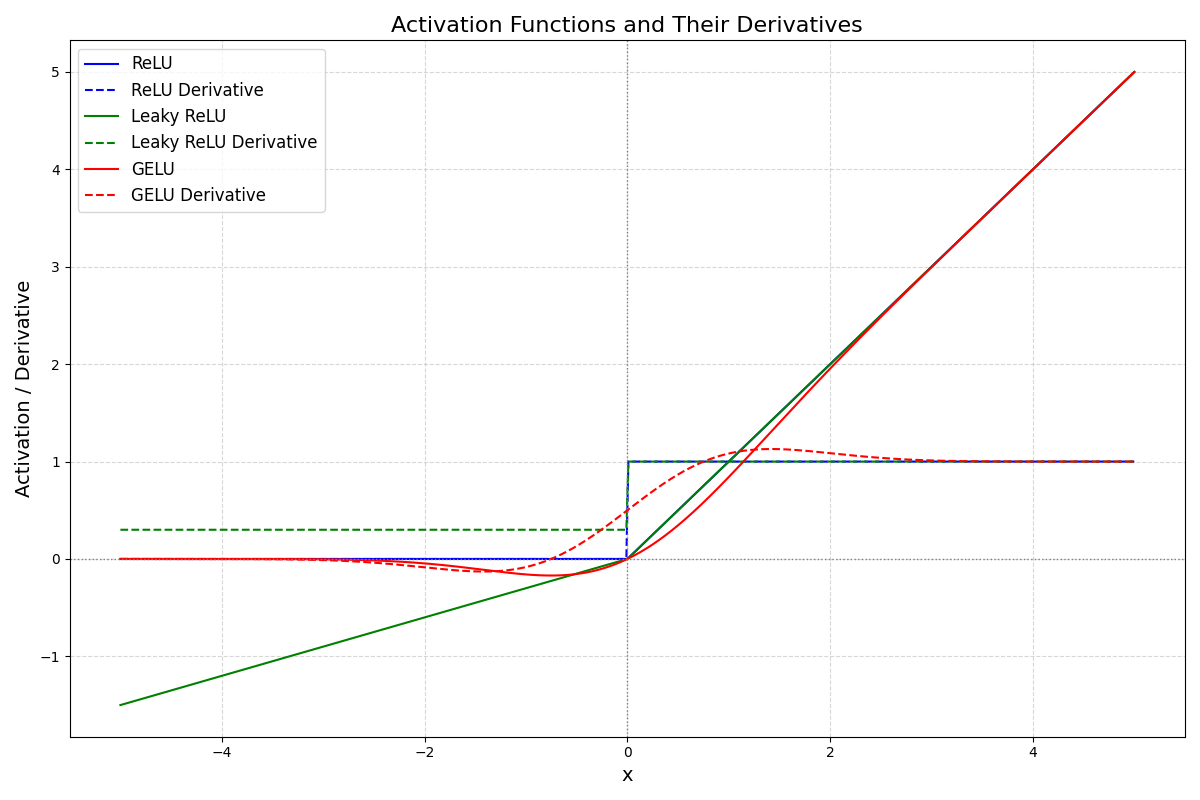
\includegraphics[width=0.7\textwidth]{images/activation_functions.png}
    \caption{Some activation functions and their derivatives: ReLU (blue), leaky ReLU (green, slope of 0.3), GELU (red).}
    \label{fig:activation}
\end{figure}

Another commonly used function is the sigmoid function, which is bounded between 0 and 1, given by
\begin{equation}
  f (x) = \frac{1}{(1 +e^{−x})},
\end{equation}
which is mainly used in the output layer of NNs built for binary classification, so that the output can be directly interpreted as a probability. The generalisation of this function, called the softmax function, is used when the classification is multinomial and multiple outputs are present. It is defined as:
\begin{equation}
    f (x_{i}) = \frac{e^{x_{i}}}{\sum_{j}e^{x_{j}}},
\end{equation}
ensuring that the sum of the outputs corresponding to all classes equals 1, and that individual outputs can also be interpreted as the probability of belonging to each class.

\subsection{Regularization}

Although regularisation techniques such as L2 regularisation, dropout, or normalisation layers are often employed to mitigate overfitting in neural networks, they are not explicitly used in the training strategy followed in this thesis. Nevertheless, the underlying principle remains the same: to increase the generalisation power of the model and avoid learning noise or fluctuations specific to the training dataset.

In this thesis, batch normalisation~\cite{ioffe2015batchnormalizationacceleratingdeep} is applied as the only regularisation-related technique. It operates by rescaling and shifting the inputs of each layer such that, within each training mini-batch, they are normalised to have approximately zero mean and unit variance. This standardisation is performed independently for each feature, which helps to stabilise and accelerate the training process. In addition, it enables the use of larger learning rates and reduces the sensitivity to weight initialisation. In contrast to layer normalisation, which normalises each training example across all of its features, batch normalisation uses the distribution of values over the examples contained in the mini-batch. This reliance on batch-level statistics is particularly effective in deep networks trained with mini-batch stochastic gradient descent.

\subsection{Optimization and Training}

As previously discussed, the loss function guides the learning process of the neural networks implemented in this work. The optimisable parameters of the algorithm considered here are updated using an optimiser. A wide range of optimisers exists, many of which are based on Stochastic Gradient Descent (SGD), which essentially computes the gradient of the loss function with respect to these parameters.

Aiming to minimise the loss function, the parameters are updated at each step in the negative gradient direction as follows (for a single parameter):
\begin{equation}
    \theta_{i+1} = \theta_{i} - \eta \Delta_{\theta}\mathcal{L}_{\theta}(\hat{\vec{y}},\vec{y}),
\end{equation}
where $\theta_{i}$ is the learnable parameter at step $i$, and $\eta$ is the learning rate (LR), which defines the step size. In this thesis, an extension of the SGD optimiser called $Adam$~\cite{kingma2017adammethodstochasticoptimization} is used.

Since analytical computation of the gradients is not feasible, the backpropagation algorithm~\cite{Rumelhart1986LearningRB} is employed. It efficiently computes these gradients by propagating the computation backwards from the output layer to the input.

Finally, it is during the training itself that the learnable parameters are optimised based on the input data. Information is passed to the algorithm in small subsets of data, the so-called batches. The value of the loss function is computed on each batch and used to update the network's parameters, aiming to reduce the loss function as described.

This process is repeated for all the batches into which the original dataset has been divided, completing what is known as one $epoch$. After each epoch, the performance of the neural network is evaluated on the validation dataset. This procedure is repeated for the agreed number of epochs, and the model that performs best in terms of validation loss is finally retained.

Regarding the implementation of the architecture and its optimisation, there are many software libraries available for machine learning, with \textsc{tensorflow}~\cite{tensorflow2015} and \textsc{pytorch}~\cite{pytorch} being among the most widely used. The NN model developed in this thesis (Section~\ref{subsec:dnn_id}) was implemented using \textsc{TensorFlow} version 2. Since these frameworks are not natively compatible with the ATLAS software environment, the \textsc{lwtnn}~\cite{lwtnn,lwtnn2} package was originally developed to facilitate the integration of neural networks into the ATLAS software.

\subsection{Input Data and Preprocessing}
\label{dnn:preprocessing}

A common issue when directly feeding a DNN with the collected training input dataset is that the algorithm might learn specific features that are either irrelevant or not fully representative of what is expected in real data. This can lead to a degradation in performance. To mitigate such effects, a data preprocessing step is introduced before passing the input to the algorithm.

Applying scaling or certain transformations to the input data is generally beneficial in most cases. In general, DNNs tend to perform better when input features are of order one. This significantly improves the stability of the training process, its speed and efficiency, and ultimately the final performance of the algorithm.

A simple way to illustrate this is to consider a NN with two inputs, $x_{1}=1$ and $x_{2}=100$. In the first hidden layer, each node combines these inputs as $w_{1}x_{1} + w_{2}x_{2}$, where $w_{1}$ and $w_{2}$ are the weights. These typically start with similar values during optimisation, so due to the large difference in the input values, $x_{1}$ contributes very little to the DNN. The optimisation process may fail to balance both contributions effectively.

Transformations or scalings such as those implemented in the \textsc{scikit-learn} package~\cite{scikitlearn} can address this issue. In this thesis, only the \texttt{QuantileTransformer} is used. This method performs a monotonic, non-linear transformation that maps the input distribution of each variable to a uniform distribution between zero and one, based on empirical quantiles. This approach effectively handles outliers and compresses extreme values but may introduce distortions in the correlations between input variables.

It also happens that in some cases, certain input variables play a critical role in defining the phase space of the problem or guiding the algorithm’s learning process, but they should not directly influence the classification decision. A clear example in this thesis involves the pseudorapidity ($\eta$) and transverse momentum ($p_{\text{T}}$) of electron candidates. The features of signal and background electrons vary significantly with respect to these two variables, which can cause the model to favour certain regions of $\eta$ or $p_{\text{T}}$, introducing an unwanted bias.

To prevent this, two main strategies are adopted. The first consists in the targeted removal of candidates from overrepresented regions of specific classes, ensuring a more balanced overall distribution. The second strategy applies reweighting factors to the distributions of the other input variables so that the shapes match across all classes. These two methods can be combined to achieve better balancing.

Another frequent source of bias occurs when the training dataset is dominated by a particular class. In such cases, the model tends to assign higher classification scores to this class by default, even when the discriminating features are weak. This imbalance can significantly compromise performance, especially in multiclass classification. The same strategies described above can be extended to address this issue and ensure a more balanced training.



\section{Boosted Decision Trees}
\label{sec:bdt_general}

Boosted Decision Trees (BDTs)~\cite{bdts} are among the most widely used machine learning algorithms in high energy physics. They are based on a structured set of decision trees that use the boosting technique to enhance classification performance. Instead of relying on a single decision tree, which tends to overfit and lacks generalisation, BDTs combine the output of many weak classifiers to form a more powerful model.

Each decision tree consists of a sequence of binary splits that partition the input phase space according to a given set of input variables. At each node of the tree, a discriminating variable and an optimal threshold are selected to best separate the events of two classes, for the case of binomial BDTs. The metric most commonly used to determine the optimal split is the $Gini$-index~\cite{gini}, defined as:

\begin{equation}
G = \sum_{i} p_i (1 - p_i),
\end{equation}

where $p_i$ represents the purity of class $i$ in a given node. The $Gini$-index quantifies the degree of mixing between different classes: lower values indicate purer nodes and thus more efficient separations. The tree continues splitting recursively until a predefined stopping criterion is met, such as a minimum number of events per node or a maximum depth. The result is a decision tree that divides the input space into regions classified as signal- or background-like.

However, a single tree has limited power and is prone to fluctuations in the training data. To improve the generalisation, the boosting technique is applied. In this approach, multiple trees are trained sequentially, each focusing on the events that were misclassified by the previous ones. The so-called boosting process assigns higher weights to those events which are difficult to classify in subsequent trees.

In this work, BDTs are implemented using the \textsc{tmva} package from the \textsc{root} framework~\cite{tmvatoolkit}, which employs its own GradientBoost method, minimizing a loss function by iteratively adding trees to correct the errors of the ensemble. 
The performance of this algorithm is governed by several hyperparameters, such as the learning rate, 
the maximum depth of the trees, and the total number of trees. However, in analyses with limited 
statistics, like the one presented in this thesis, there is little benefit from an extensive optimisation 
of these hyperparameters. In such cases, the training tends to be more affected by statistical fluctuations 
than by the fine-tuning of the model configuration.

While the original formulation of BDTs is focused on binary classification, the present work employs the multiclass extension of the method~\cite{tmvatoolkit}. In this case, the algorithm assigns to each input a set of scores corresponding to each of the target classes, and the final classification is obtained by selecting the class with the highest score. This approach enables a single training to distinguish between multiple physics processes simultaneously, offering a powerful tool for complex analyses.





%-------------------------------------------------------------------------------

%-------------------------------------------------------------------------------
\chapter{Electron Reconstruction, Identification and Efficiency Measurements}
\label{chap:electrons}
\newcommand*{\zee}{$Z \to e^{+}e^{-}$\xspace}
\newcommand*{\et}{$E_{\text{T}}$\xspace}
\newcommand*{\zmass}{$\texttt{Z}_{\text{mass}}$\xspace}
\newcommand*{\ziso}{$\texttt{Z}_{\text{iso}}$\xspace}
\newcommand*{\tp}{T$\&$P\xspace}
\newcommand*{\et}{$E_{\text{T}}$\xspace}
\newcommand*{\eta}{$\eta$\xspace}

\setcounter{secnumdepth}{3}

Electrons play a crucial role in the ATLAS physics programme, appearing in key final states from precision electroweak measurements to Higgs boson studies and BSM searches. For this reason, accurate reconstruction, identification, calibration and isolation are critical to achieving the ATLAS experiment’s scientific goals.  

Although the basic workflow for constructing electron candidates mirrors the one already explained for other physics objects in Chapter~\ref{chap:object_rec}, the performance demands on electrons are particularly stringent, starting from the precision in which tracks and energy clusters are reconstructed to achieving the best possible agreement between recorded data and the Monte Carlo simulations.  

In the following chapter, the treatment, definition, and calibration of electrons in ATLAS are discussed, especially because part of the work in this thesis has focused on the study and refinement of a DNN for electron identification and classification against other objects that can mimic their signature.  The architecture of this ML algorithm is going to be shown, as well as the electron features that are used as inputs, its performance, and how its output is handled. 

This DNN is introduced as an improved method intended to replace the likelihood-based approach employed since the beginning of Run~2~\cite{Aad:2684552,Aaboud:2657964}, which is also discussed here.  Finally, efficiency measurements are compared for prompt electrons obtained with both techniques and derive scale factors to correct any mismatches between the performance in data and MC simulation.  These efficiencies are measured in data using tag-and-probe techniques on a pure and unbiased sample of electrons, typically drawn from well-known physics processes rich in prompt electrons such as the $Z\to e^+e^-$ decay, an example of which is illustrated in the event display in Figure~\ref{fig:zee}.

\begin{figure}[htbp]
    \centering
    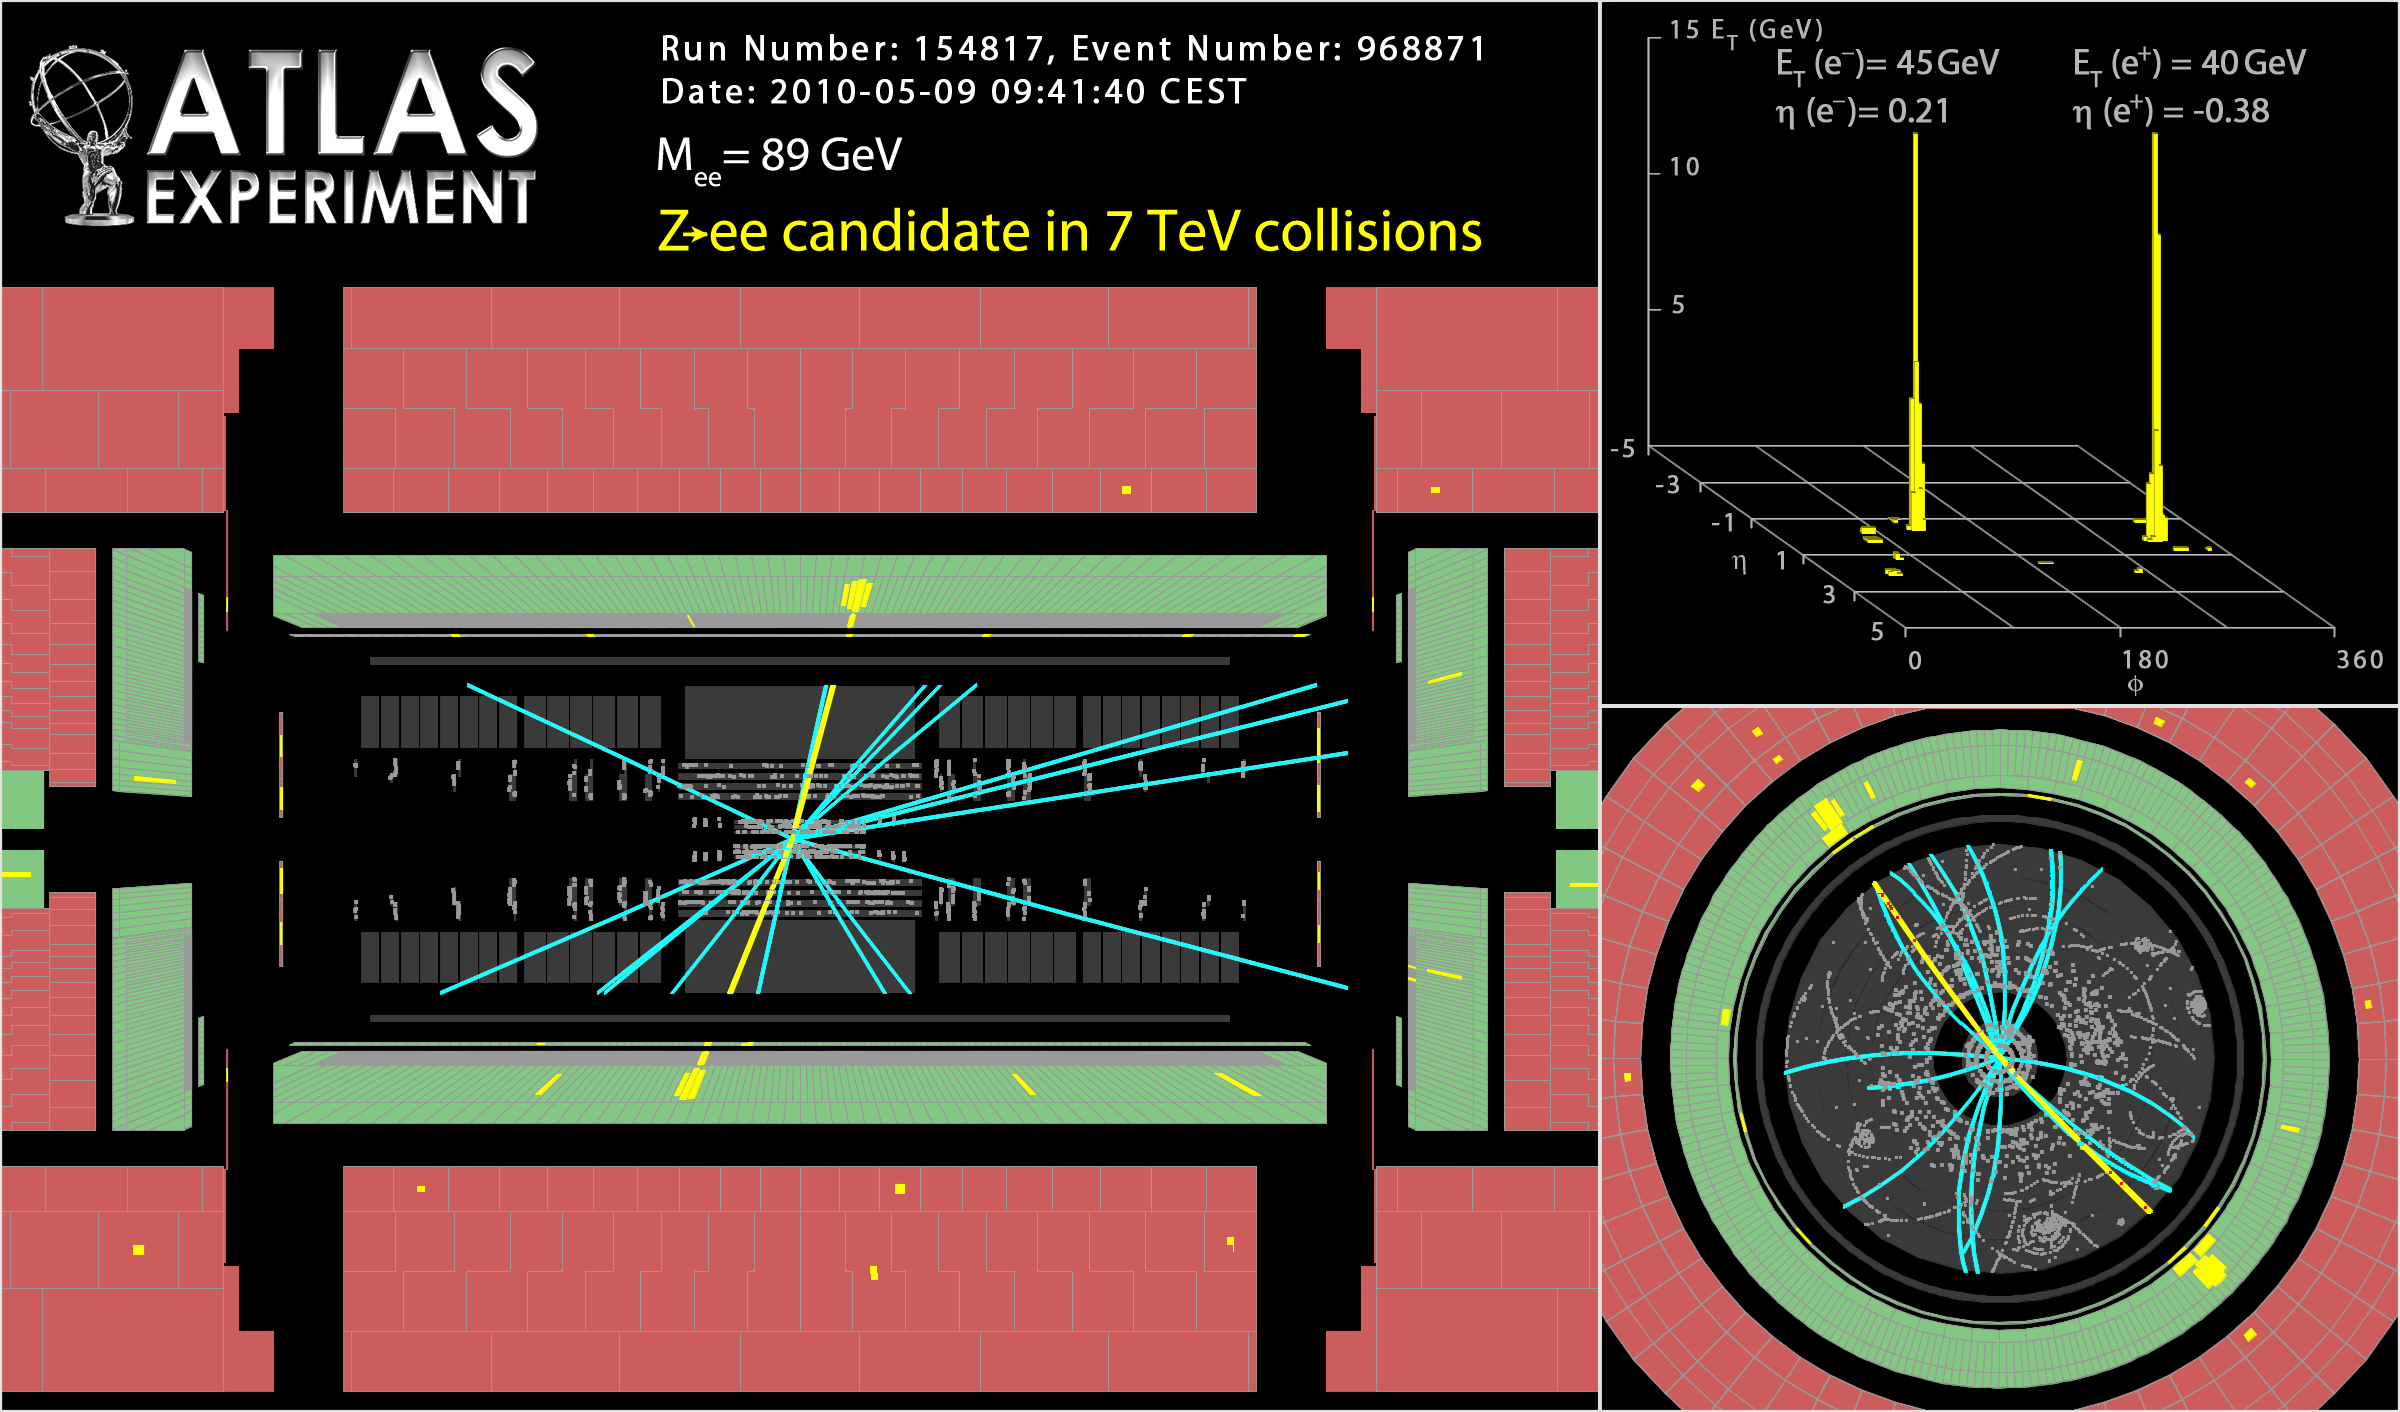
\includegraphics[width=0.7\textwidth]{images/Zee.png}
    \caption{ATLAS reconstructed event display, collected on 9 May 2010, of a candidate for a $Z\to e^+e^-$ decay. The two electrons are well isolated and represented with yellow lines. Further event properties: $p_{\text{T}}(e^{+})$ = 40~GeV, $p_{\text{T}}(e^{-})$ = 45~GeV, $\eta(e^{+}) = -0.38$, $\eta(e^{-}) = 0.21$, $m_{e^{+}e^{-}}=89$~GeV~\cite{atlas:eventdisplay}. }
    \label{fig:zee}
\end{figure}

The rest of this chapter covers the reconstruction inputs and calibration steps that define electrons in ATLAS, the architecture and training of the new DNN identification algorithm, the tag-and-probe procedures used to extract data-driven efficiencies. Finally, a direct comparison of DNN identification performance against the Run-2 likelihood benchmark is presented. Together, these studies quantify the improvements in signal efficiency and background rejection achieved by the neural-network approach and lay the groundwork for its deployment in Run-3 analyses.  

%%%%%%%%%%%%%%%%%%%%%%%%%%%%%%%%%%%%%%%%%%%%%%%%%%%%%%%%%%%%%%%%%%%%%%%%%%%%%%%%%%%%%%%%%%%%%%%%%%%%%%%%%%%%%%%%%%%%%%%%%%%%%%%%%%%%%%%%%%%%%%%%%%%%%%%%%%%%%%%%%%%%%%%%%%%%%%%%%%%%%%%%%%%%%%%%%%%%%%%%%%%%
\section{Electron Reconstruction}
\label{sec:electron_reconstruction}

In the ATLAS detector, an electron can be reconstructed when its electromagnetic energy deposits in the calorimeter system can be matched to a charged-particle track in the ID. Figure~\ref{electron_journey} illustrates the typical journey of an electron traversing the various layers of ATLAS, from the interaction point outwards.

\begin{figure}[htbp]
  \centering
  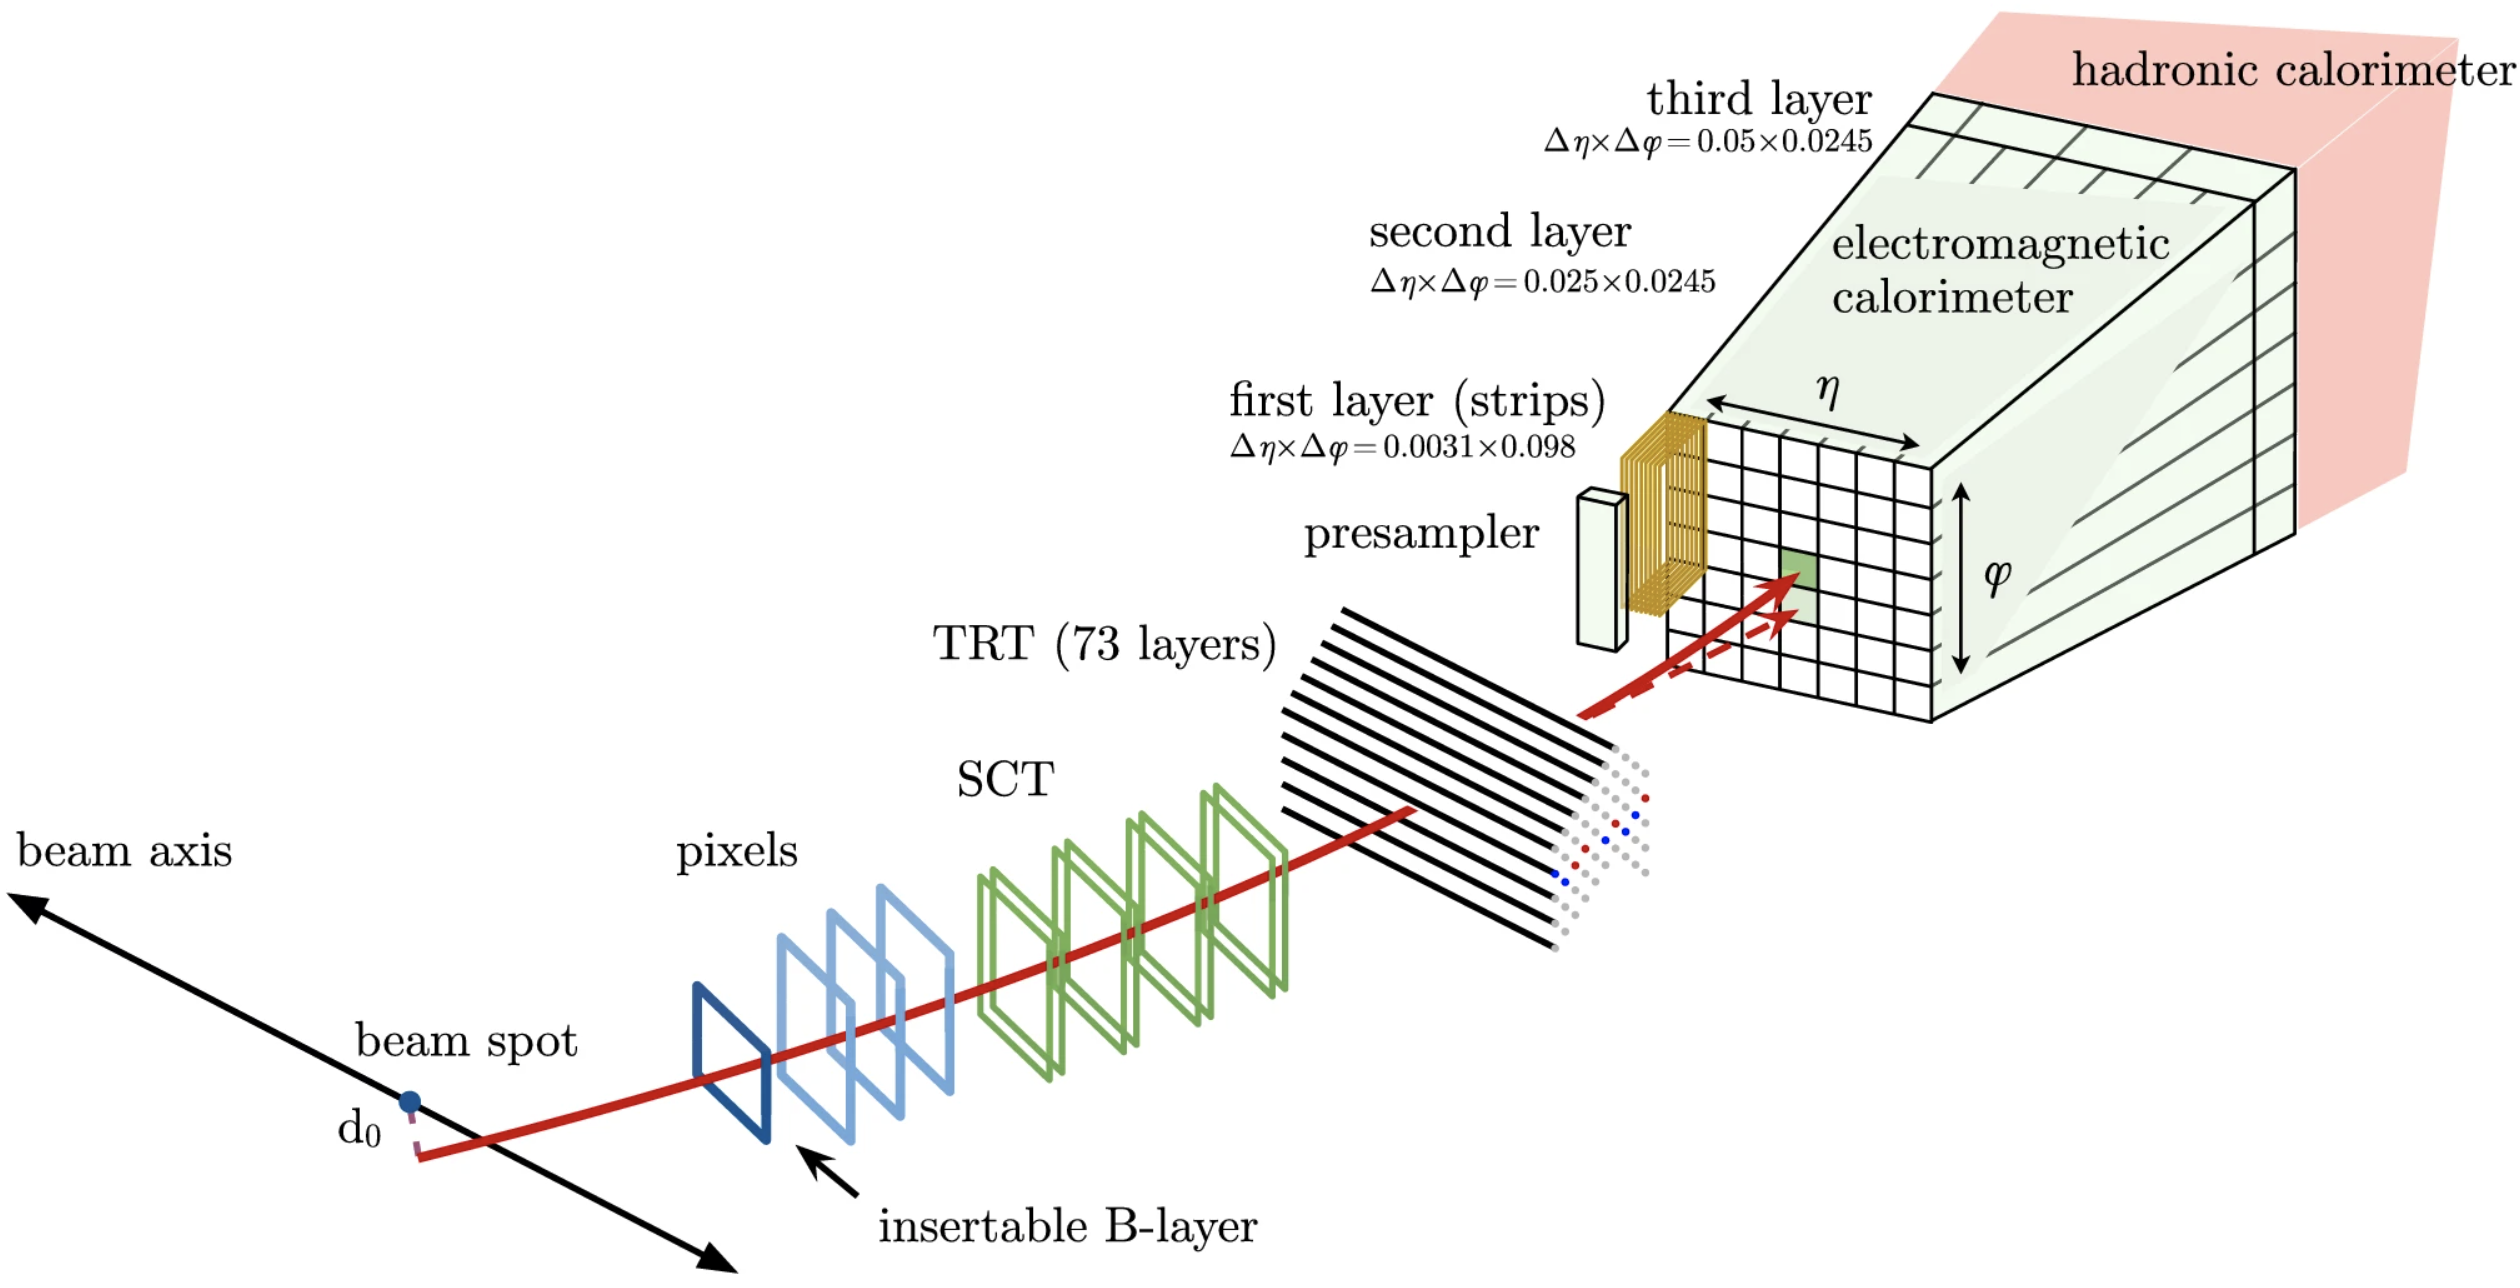
\includegraphics[width=0.9\textwidth]{images/electron_journey.png}
  \caption{Illustration of the typical journey of an electron passing through ATLAS. In red it is represented its expected path, first going through the tracking system. Afterwards it leaves mostly all its energy in the electromagnetic calorimeter. It can be also found the possible path (dashed red) of photon radiated by bremsstrahlung when the electron interacts with the material~\cite{Aaboud:2657964}.}
  \label{electron_journey}
\end{figure}
Although the electron first traverses the ID before depositing most of its energy in the electromagnetic calorimeter, the reconstruction of an electron candidate actually begins with the identification of energy clusters in the EM calorimeter. After the clustering step, 
the tracks in the ID are reconstructed and classified, as detailed in Section~\ref{sec:tracks}. The final step is to efficiently match these tracks to the electromagnetic clusters to form electron candidates, being able to distinguish them from other objects such as charged pions.

\subsection{Cluster Building}

The dynamic algorithm for defining variable-size clusters of cells from the calorimeters was implemented in Run-2~\cite{dyn_clust}, yielding performance that far surpasses the fixed-size algorithm used in the previous data-taking period~\cite{fix_clust}.

These dynamically sized clusters, known as topological clusters (topoclusters), grow around a seed cell defined according to an algorithm detailed in Ref.~\cite{fix_clust}. A seed must satisfy a cell Energy–momentum significance of $\epsilon_{\text{cell}}^{\text{EM}} \geq 4$
and cannot be located in the presampler or the first layer of the electromagnetic calorimeter. This significance is defined as
\begin{equation}
  \epsilon_{\text{cell}}^{\text{EM}} = \frac{E_{\text{cell}}^{\text{EM}}}{\sigma^{\text{EM}}_{\text{noise,cell}}},
\end{equation}
being \(E_{\text{cell}}^{\text{EM}}\) the energy of the given cell and \(\sigma^{\text{EM}}_{\text{noise,cell}}\) its expected noise.

The significance of all cells neighboring the seed cell is then evaluated, and any cell with $\epsilon_{\text{cell}}^{\text{EM}} \geq 2$ is added to the cluster. This procedure iterates, treating each newly added cell as the seed for the next step, forming a growing protocluster. Protoclusters sharing a cell are merged together, and once no further high-significance cells can be included, a final growth step adds all adjacent cells regardless of their significance. If the resulting topocluster contains more than one local maximum, it is split into separate clusters, each centered on one maximum cell. A local maximum is defined as a cell with \(E_{\text{cell}}^{\text{EM}}>500\)~MeV that has at least four neighbors of lower energy.

Contributions from the presampler and the first EM layer are also added when computing the cluster’s electromagnetic energy. The electromagnetic fraction, \(f_{\text{EM}}\), is defined as the ratio of this EM energy to the cluster’s total energy. To suppress clusters from pile-up or hadronic activity, only those with \(f_{\text{EM}}>0.5\), \(E_{\text{EM}}>400\)\,MeV, and at least half of their energy in the EM calorimeter are retained as electron candidates.  

\subsection{Track-to-Cluster Matching}

For electron candidates, the standard tracking algorithm explained in Section~\ref{sec:tracks} is extended to account for electrons losing energy via bremsstrahlung as they traverse the ID material. 

Initially, tracks are fitted under a pion hypothesis assuming an ideal helical trajectory~\cite{tracks}. If this fit fails for a given track seed within the region of interest defined by the EM topocluster (i.e., small pseudorapidity separation between track and cluster), the fit is retried with a modified pattern-recognition algorithm based on the Kalman filter formalism~\cite{FRUHWIRTH1987444}, which allows for energy losses at each material intersection due to photon radiation and thus deviations from a perfect helix.

This formalism, called Gaussian Sum Filter (GSF), represents the track state as a weighted sum of Gaussian components, each propagated in parallel via a Kalman filter, modelling the sudden curvature changes induced by discrete photon emissions. After GSF refitting, the tracks are extrapolated to the EM calorimeter and matched to EM topoclusters using asymmetric $\phi$ windows (wider on the side corresponding to expected energy loss) and tight $\eta$ proximity. When multiple tracks match a single cluster, candidates are ranked first by fit quality and then by distance to the cluster barycentre in the second EM layer; the highest-ranked track is chosen to define the electron $\eta$ and $\phi$ coordinates.


\subsection{Superclusters and calibration}

In order to capture the full energy deposited by these bremsstrahlung photons from the electron candidate, adjacent EM topoclusters are merged into superclusters, which gather all significant energy deposits along the electron’s radiative path, as represented in Figure~\ref{fig:superclust}~\cite{Aad:2684552}.
\FloatBarrier
Reconstruction of an electron supercluster begins by ordering all electromagnetic topoclusters by their transverse energy and selecting the highest-$E_{\text{T}}$ cluster as the seed. This seed must not already be assigned to another supercluster, and the reconstructed track matched to it must carry at least four hits in either the Pixel or the SCT detectors~\cite{Aad:2684552}. Once a valid seed is identified, additional “satellite” topoclusters are incorporated within a sliding window of \(\Delta\eta\times\Delta\phi = 0.075\times0.125\) and \(0.125\times0.300\), centered on the seed’s energy-weighted barycenter. The smaller window captures nearby secondary electromagnetic showers, while the larger one recovers energy radiated via bremsstrahlung. Finally, the assembled supercluster is matched to its track using the same \(\eta\)-\(\phi\) proximity criteria described before, yielding the fully reconstructed electron object used in subsequent physics analyses.  

\begin{figure}[htbp]
  \centering
  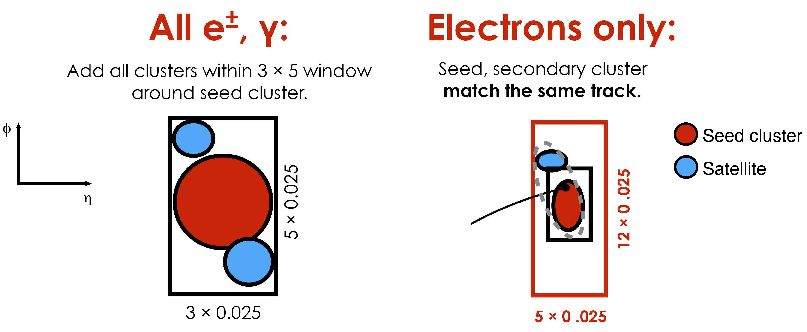
\includegraphics[width=0.8\textwidth]{images/superclusters.png}
  \caption{Schematic overview of the formation of superclusters during electron reconstruction~\cite{Aad:2684552}.}
  \label{fig:superclust}
\end{figure}

However, this reconstruction procedure is based on the raw energy measurements of both electrons and photons, derived from the sum of cell energies. To achieve the highest possible precision, these energy measurements must be calibrated. First, a BDT regression is trained on Monte Carlo simulation, combining the energy deposits across the three longitudinal calorimeter layers. Subsequently, the response of each individual layer is calibrated separately to correct for its \et-dependent behavior, and the same corrections are applied identically to both data and simulation samples.

After the layer-by-layer corrections, residual discrepancies between data and simulation (arising from effects such as azimuthal non-uniformities in the calorimeter's granularity) are removed by applying additional region-dependent corrections to the data. Finally, the absolute energy scale and resolution are tuned using large samples of \(Z\to e^+e^-\) events, ensuring that the reconstructed \(Z\) peak in data aligns with the simulation. Any remaining resolution differences are corrected by smearing the energy in MC simulations. The overall procedure is validated and its uncertainties quantified using \(J/\psi\to e^+e^-\) events.  

Finally, it is worth noting that the reconstructed electron four-momentum is obtained by combining the calibrated energy of the matched supercluster with the direction provided by the associated track at the interaction point, yielding a precise description of the candidate’s kinematics.

For efficiency measurements and scale-factor computations, which will be discussed in Section~\ref{sec:electron_efficiency_measurements}, the so-called ``detector'' pseudorapidity is employed, defined as the pseudorapidity of the energy barycentre in the second layer of the EM calorimeter of the primary cluster. Since this layer contains the bulk of the electron energy deposition, this observable provides a robust proxy for the cluster location in the calorimeter and is therefore used to parameterise efficiencies and data-to-MC corrections.

This section is concluded by noting that the concept of transverse energy does not have a direct physical meaning, but is conventionally defined as $E_{\text{T}} = E \cdot \sin\theta$. For electrons, whose mass is negligible compared to their energy, this definition leads to values that are identical to the transverse momentum $p_{\text{T}}$. Consequently, both notations are used interchangeably throughout the following sections of this work.

%%%%%%%%%%%%%%%%%%%%%%%%%%%%%%%%%%%%%%%%%%%%%%%%%%%%%%%%%%%%%%%%%%%%%%%%%%%%%%%%%%%%%%%%%%%%%%%%%%%%%%%%%%%%%%%%%%%%%%%%%%%%%%%%%%%%%%%%%%%%%%%%%%%%%%%%%%%%%%%%%%%%%%%%%%%%%%%%%%%%%%%%%%%%%%%%%%%%%%%%%%%%
\section{Electron Identification}

As already mentioned, there are other types of physics objects that can mimic the characteristic signature left by electrons in the ATLAS detector, and can therefore end up being reconstructed as electron candidates. 

In the physics analyses carried out within the collaboration, the background coming from these objects needs to be reduced as much as possible. Moreover, not all genuine electrons are to be considered as signal in many cases. Only prompt isolated electrons originating from the decay of heavy bosons such as the $W$, $Z$, and Higgs bosons are of interest, while those coming from the decay of charged quarks or photon conversions are generally considered as background.

Therefore, in order to efficiently classify the electron candidates, a set of selections must be applied after reconstruction, which is what is known as identification. To identify the types of electrons, discriminants are typically defined based on observables or features of the physical objects that allow for a discrimination between prompt and background electrons, for instance.

These discriminants can be defined in various ways, and Section~\ref{LH_identification} describes the Likelihood-based approach, used since the beginning of the Run-2 period, and the novel identification algorithm based on a DNN is described in Section~\ref{subsec:dnn_id}.

Finally, the identification process is completed by using the output of that discriminant, on which certain thresholds are defined targeting specific values of signal identification efficiency and background rejection. Since the behaviour of electrons generally varies as a function of their energy and of the detector region under consideration, these thresholds are typically defined in bins of the electron’s \et and $\eta$, and are encapsulated in what are known as identification Working Points (WPs). These WPs generally also include requirements on additional variables, as described below. The different WPs obtained from the same discriminant are grouped into identification menus, which are ultimately provided for general physics analysis use.

\subsection{Likelihood-based identification}
\label{LH_identification}
So far, electron identification in ATLAS has been based on a Likelihood (LH) approach~\cite{Aad:2684552,Aaboud:2657964}, which relies on a wide range of information from different detector subsystems. This algorithm uses high-level input variables defined from the properties of electrons and the information they leave as they pass through the detector. These variables will be detailed later, since they are largely shared with the DNN, and further information can be found in Ref.~\cite{Aaboud:2657964}.

A central aspect in the construction of the LH discriminant is the definition of one-dimensional Probability Density Functions (PDFs) for each input variable. It is done separately for signal and background electrons, based either on real data or on simulations.
The discriminant is constructed from these PDFs, which reveals one of the limitations of this method: the correlations between variables are lost when creating these density functions, which are obtained by applying a Kernel Density Estimator (KDE) to the histograms of each variable separately, using the TMVA toolkit~\cite{tmvatoolkit}. 

Therefore, the likelihood of an electron candidate being signal ($L_{\text{S}}$) or background ($L_{\text{B}}$) is given by:

\begin{equation}
  L_{\text{S(B)}} (\textbf{x}) = \prod_{i} P_{\text{S(B)},i}(x_{i}),
\end{equation}
where $P_{\text{S(B)},i}(x_{i})$ are the signal (background) PDFs, and $x_{i}$ is simply the value of the $i$-th input variable, so the likelihood is just the product of all PDFs.
Then, the likelihood discriminant, $d_{L}$, is simply obtained as:
\begin{equation}
  d_{L} = \frac{L_{\text{S}}}{L_{\text{S}} + L_{\text{B}}},
\end{equation}
which achieves the goal of clearly separating the signal and background distributions, as can be seen in the example shown in Figure~\ref{fig:lhdis}.
\begin{figure}[htbp]
  \centering
  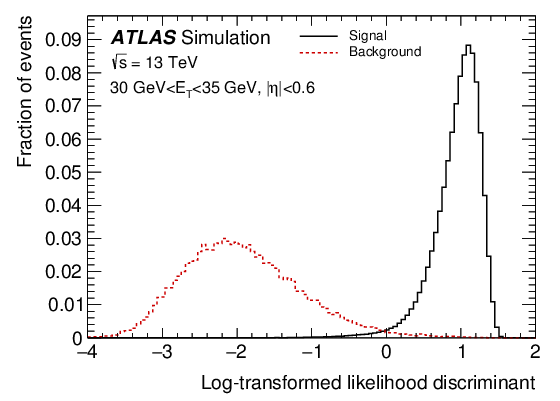
\includegraphics[width=0.6\textwidth]{images/lhdis.png}
  \caption{Likelihood discriminant distributions obtained in a particular \et and $\eta$ bin, for signal and background computed for simulated electrons corresponding to rel.21 Run-2~\cite{Aaboud:2657964}.}
  \label{fig:lhdis}
\end{figure}

As previously mentioned, the PDFs of the variables are parametrised in different bins of \et and $\eta$, and the same applies when building the discriminant and defining the thresholds that form the WPs.

The additional requirements to these cuts on the discriminant, and applied to determine whether an electron candidate passes a given WP, include a certain number of hits in different parts of the tracking detectors and also requirements on the ambiguity type. This ambiguity type is a flag assigned to the candidate during reconstruction, providing information on whether the topocluster associated with the electron was also reconstructed as a photon.
Each WP encapsulates different requirements, and in this thesis $LHLoose$, $LHMedium$, and $LHTight$ are used, ordered from highest to lowest signal identification efficiency, and the reverse in terms of background rejection. They are subsets of each other, meaning that if an electron passes $LHTight$, it also passes the other two WPs.

Regarding the LH menu used later in this thesis in the efficiency and scale factor calculations, the probability density functions (PDFs) were derived directly from collision data. Signal PDFs are taken from data to guarantee the best possible performance when applied to real events. Background PDFs are also extracted from data, since they lead to distributions that are less signal-like than those obtained from Monte Carlo. This behaviour is precisely what is desired for the likelihood method to achieve an efficient discrimination.

The selection used to obtain the purest possible sample of candidates for both types is fully detailed in Ref.~\cite{lucas_thesis}. In summary, in order to construct the PDFs, a tag-and-probe method is applied. Signal electrons are selected from $Z \rightarrow e^{+}e^{-}$ or $J/\psi \rightarrow e^{+}e^{-}$ decays. Events with $E_{\text{T}} > 15$~GeV are taken from $Z$ decays, while lower-$E_{\text{T}}$ electrons ($E_{\text{T}} \leq 15$~GeV) come from $J/\psi$ decays. A tightly identified and isolated “tag” electron is required, and a “probe” electron is selected if the invariant mass of the pair matches the $Z$ or $J/\psi$ boson mass. No further identification or isolation requirements are applied to the probe, ensuring unbiased selections.

Background PDFs are obtained from multi-jet events in data. Due to their large cross-section, loose selection of reconstructed electrons yields mostly background. To improve purity, $Z \rightarrow e^{+}e^{-}$ and $W \rightarrow e\nu$ decays are vetoed. The $Z$ veto removes events with a second electron forming a mass near the $Z$ boson. The $W$ veto applies a cut on the transverse mass, which also removes electrons from top-quark decays.


\subsection{Deep neural network for electron identification}
\label{subsec:dnn_id}
%Small introduction about the DNN: why is a good alternative? Reference the DNN paper, and the Statistical methods section for more info about DNNs. Talk a bit about what is going to be shown heres

Electron identification in ATLAS has historically been performed without the use of machine learning. During the Run-1 period, a cut-based selection was used, applying rectangular cuts directly optimised on characteristic observables of the electron candidates. Later, during Run-2, the strategy evolved into the LH approach, described in the previous section.

While the LH method has proven effective selecting signal electrons with high efficiency and background rejection, recent advances in ML have introduced new possibilities for improving classification performance and signal-to-background discrimination in high energy physics. In particular, deep neural networks (DNNs) have demonstrated a strong ability to model complex correlations among input variables, overcoming one of the main limitations of the LH model.

This section presents an alternative algorithm based on a DNN, developed as an improved replacement for the LH discriminant using a similar set of high-level input variables.

A detailed technical description of the implemented algorithm can be found in Ref.~\cite{dnn_paper}, initially developed and validated for Run-2 Release 21. More general information on the statistical principles and methodology of neural networks is provided in Section~\ref{sec:dnn_general}.

Here, the focus is placed on the specific application to electron identification, training and optimising the DNN using simulated samples to distinguish prompt isolated electrons from various background sources. The following describes the selection of samples and the definition of training classes, the choice and preprocessing of input variables, the training procedure and performance, and finally, the definition of the working points derived from the DNN output.

\subsubsection{Samples and electron selection}
%Mention that samples used here were already presented in Section~\ref{subsec:electron_mc}. Define which selection is applied to electrons used in the training, and also introduce
%how the different classes are defined. Talk about how input n-tuples are produced a bit.
The first step to prepare the DNN for electron identification is to define the training, validation, and test datasets that will feed the algorithm. As previously mentioned, simulated electron candidates are used for this purpose, extracted from different processes generated as described in Section~\ref{subsec:electron_mc}, corresponding to the Run-2 rel.22 period.

Signal electrons are selected from $Z \rightarrow e^{+}e^{-}$ decays, complemented with $J/\psi \rightarrow e^{+}e^{-}$ at low-\et. As sources of the main background processes that mimic electron-like signatures, a $\text{JF}17$ sample is used, complemented with a sample of simulated \ttbar events, from which only events containing at least one lepton in the final state are considered.

These samples are processed through the \textsc{TagAndProbe} analysis software, a \textsc{GitLab}~\cite{tagandprobe} project maintained by the $e/\gamma$ Combined Performance group, focused on the treatment and performance measurements of electrons and photons in ATLAS. This framework provides a convenient format for storing and classifying the electron candidates, allowing for the application of certain quality requisites.

In our case, a minimal preselection is applied, consisting of all reconstructed electrons to have \et$>4.5$~GeV, a minimum of one hit in the pixel subdetector, and at least seven hits in the silicon detector systems. Additionally, only electrons within the region $|\eta| < 2.47$ are considered. The electron candidates are corrected for energy scale and resolution, and further selection criteria are applied to reject candidates in problematic detector regions or with poorly reconstructed calorimeter clusters.

Finally, it should be stressed that, also in these studies, only electron candidates from $Z$-boson decays with \et $>15$~GeV are used, while $J/\psi$ decays are considered for candidates below this threshold. Further requirements on the origin of the electrons are applied to ensure that different types of candidates are selected from each sample, resulting in six distinct classes, which will be defined in the following.

\subsubsection{Classes}

One of the most important steps when training a supervised classifier like a DNN is the definition of the target classes. In our case, this translates into deciding which electron candidates are to be considered signal, and which ones are background. It is also important to note that different types of background electrons will have different properties similar to those of prompt electrons,
so any identification approach will exhibit a different separation power depending on the type of object that fakes the signature of prompt electrons.

This classification is far from trivial, since borderline or grey cases naturally arise in many physics contexts, and a good classification scheme should work for a wide range of analyses.
The class labels used in this study are based on a MC \textit{truth} classification, which uses information such as the origin and type of the electron, as well as those of its mother particles. 
This information is provided by the \texttt{MCTruthClassifierTool}~\cite{atlas:MCTruthClassifierTool}.

\begin{table}[h!]
  \centering
  \scriptsize
  \caption{Definition of the six different classes of electron candidates used to train the DNN and throughout this thesis. Adapted from Ref.~\cite{dnn_paper}.}
  \begin{tabular}{@{}l p{6.2cm} c c@{}}
    \toprule
    \textbf{Class} & \textbf{Description} & \textbf{Label} & \textbf{Sample} \\
    \midrule
    Prompt electrons & Electrons from prompt decays such as $Z \rightarrow ee$, $W \rightarrow e\nu$, or $J/\psi \rightarrow ee$, including FSR or bremsstrahlung if the origin is a prompt electron. Reconstructed charge must match truth one. & \texttt{El} & \begin{tabular}[c]{@{}c@{}}$Z\rightarrow ee$ \\ $J/\psi \rightarrow ee$\end{tabular} \\
    \midrule
    Charge-flips & Prompt electrons with misreconstructed charge, mostly due to tracking ambiguities. For bremsstrahlung, it is considered as truth charge the one of the original prompt electron. & \texttt{CF} & \begin{tabular}[c]{@{}c@{}}$Z\rightarrow ee$ \\ $J/\psi \rightarrow ee$\end{tabular} \\
    \midrule
    Photon conversions & Electrons from conversions of prompt photons into $e^{+}e^{-}$. Prompt photons misreconstructed as electrons are also included here. & \texttt{PC} & $\text{JF}17$, \ttbar \\
    \midrule
    Heavy-flavour electrons & Electrons from semileptonic $b$- or $c$-hadron decays. Typically non-isolated and slightly displaced. & \texttt{HF} & $\text{JF}17$, \ttbar \\
    \midrule
    Light-flavour $e/\gamma$ & Electrons or photons from light-quark hadron decays, including intermediate conversions like $\pi^0 \rightarrow \gamma\gamma$ with subsequent $\gamma \rightarrow ee$. & \texttt{LFEg} & $\text{JF}17$ \\
    \midrule
    Light-flavour hadrons & Hadrons misidentified as electrons due to anomalous energy deposits in the EM calorimeter. & \texttt{LFH} & $\text{JF}17$ \\
    \bottomrule
  \end{tabular}
  \label{tab:electron_classes}
\end{table}


The defined classes are shown in Table~\ref{tab:electron_classes}, as well as the corresponding simulated samples from which candidates are selected. The two signal-like classes, namely \texttt{El} (prompt electrons) and \texttt{CF} (charge-flip electrons), are extracted from $Z \rightarrow e^{+}e^{-}$ and $J/\psi \rightarrow e^{+}e^{-}$ events.

The remaining four background-like classes are primarily obtained from the $\text{JF}17$ sample, with the addition of the \ttbar\ sample to increase statistics for certain electron classes.

Prompt electrons are consistently treated as signal throughout this work. Conversely, electrons from photon conversions (PC), Heavy-Flavour (HF) decays, Light-Flavour hadron decays (LFEg), as well as hadrons misidentified as electrons (LFH), are always considered background. However, the classification of charge-flip electrons is less straightforward, since even if they originate from prompt processes, their charge is incorrectly reconstructed. Therefore, whether they are considered as signal or background depends on the specific physics analysis.
In single-lepton analyses, the reconstructed charge is typically irrelevant, allowing charge-flip electrons to be included as signal to increase statistics. Even in charge-sensitive analyses their impact is often small due to the low misidentification rate. However, in final states with two same-sign leptons, charge-flip electrons are treated as background, as they can mimic the signal while originating from more common SM processes.

It is interesting to dedicate a few more words to the ambiguity in the definition of electron classes. As discussed at the beginning of this section, not all electrons can be assigned to signal or background categories in a straightforward way. For example, in analyses targeting $H \rightarrow \tau^+\tau^-$ decays, electrons originating from $\tau$-lepton~\footnote{Electrons produced from in $\tau \to e \nu$ decays are denoted as $\tau_{e}$} decays, despite being slightly displaced due to the lifetime of the $\tau$-lepton, exhibit some calorimeter-based variables nearly identical to those from $Z \rightarrow e^{+}e^{-}$, except for impact parameter-related ones as shown in Figures~\ref{fig:compare} and~\ref{fig:compare2}. Relying too heavily on displacement for classification could thus reduce the efficiency for $\tau_e$. 
%METER AQUÍ UNOS PLOTS COMPARATIVOS ENTRE ZTAUTAU Y ZEE DE shower-shapeS E IMPACT PARAMETER??? O NO VALE LA PENA AHONDAR TANTO
\begin{figure}[htbp]
  \centering
  \begin{subfigure}[b]{0.495\textwidth}
      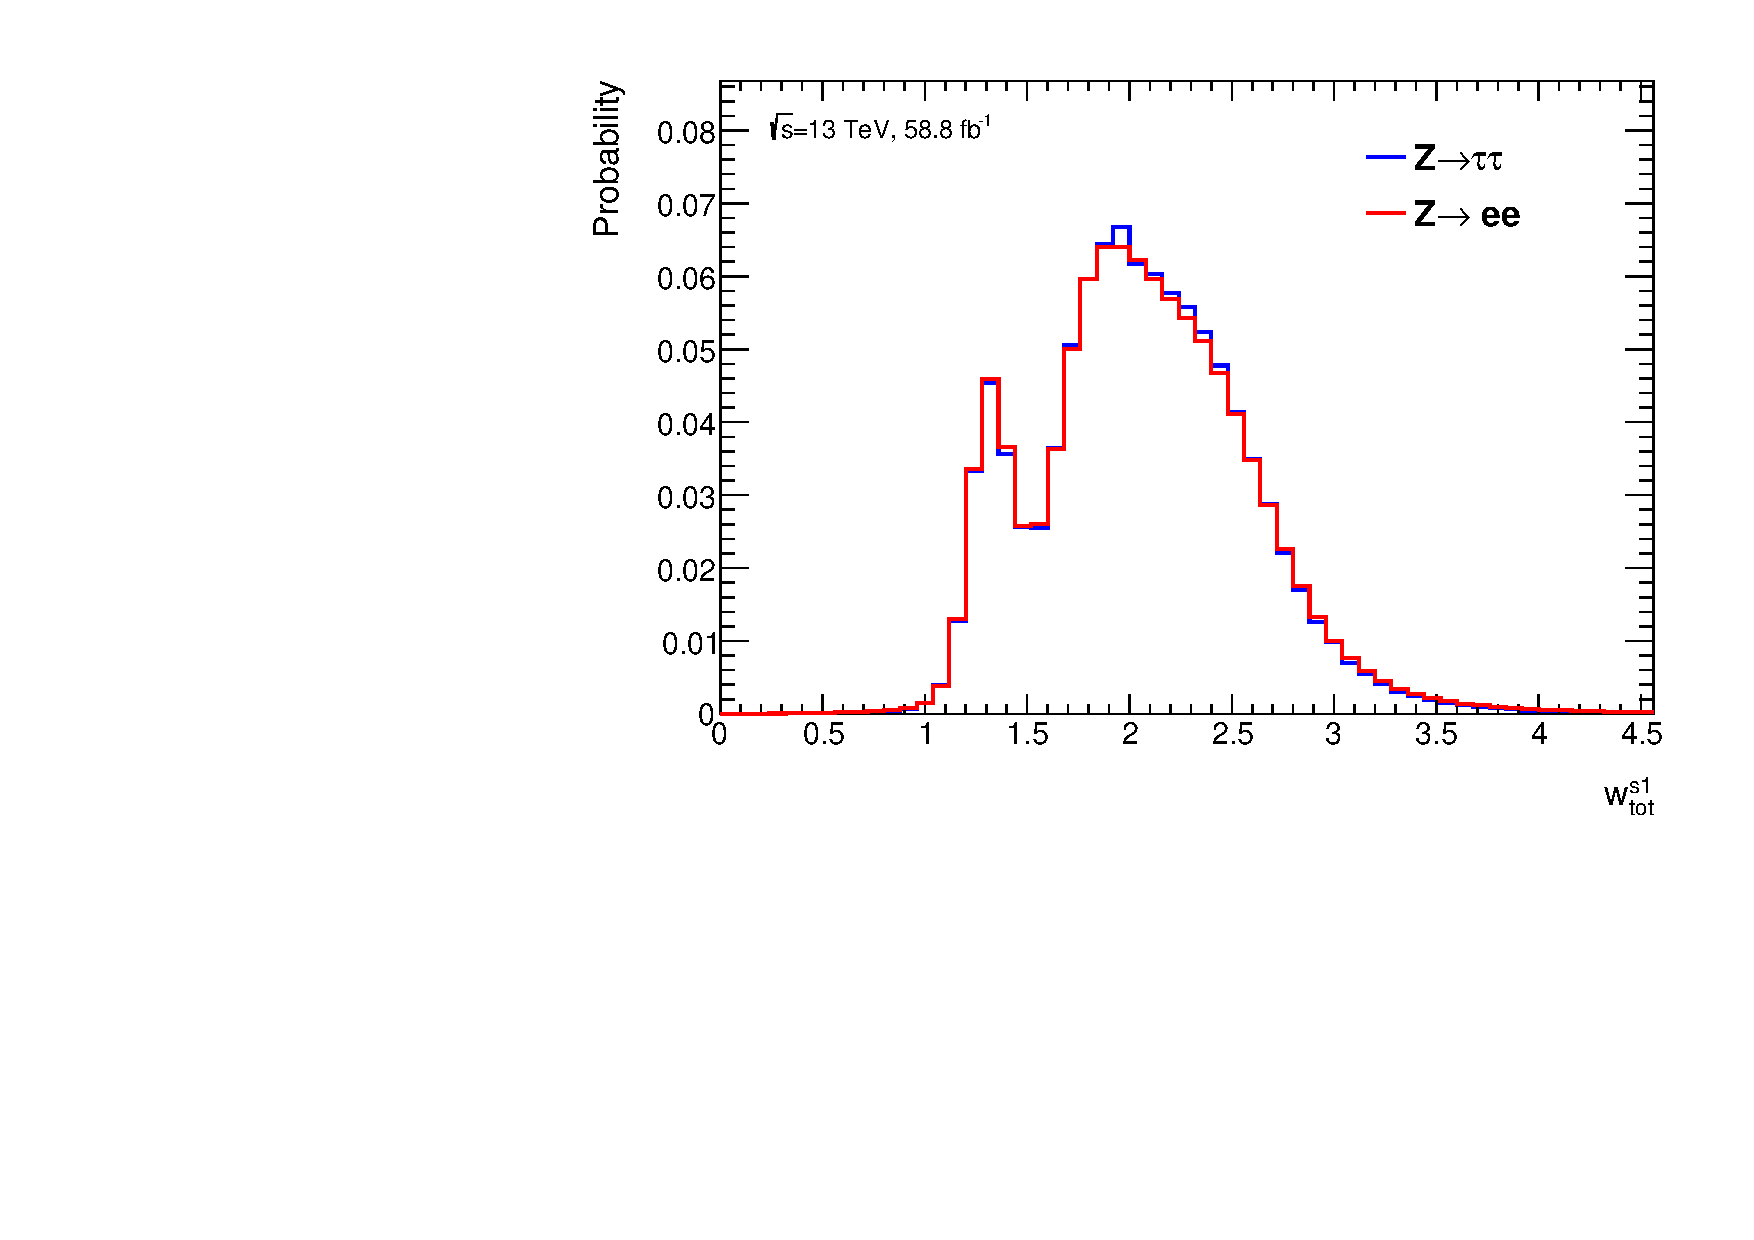
\includegraphics[width=\linewidth]{h_wtots1_Ztautau_comparison.pdf}
      \caption{}
  \end{subfigure}
  \begin{subfigure}[b]{0.495\textwidth}
      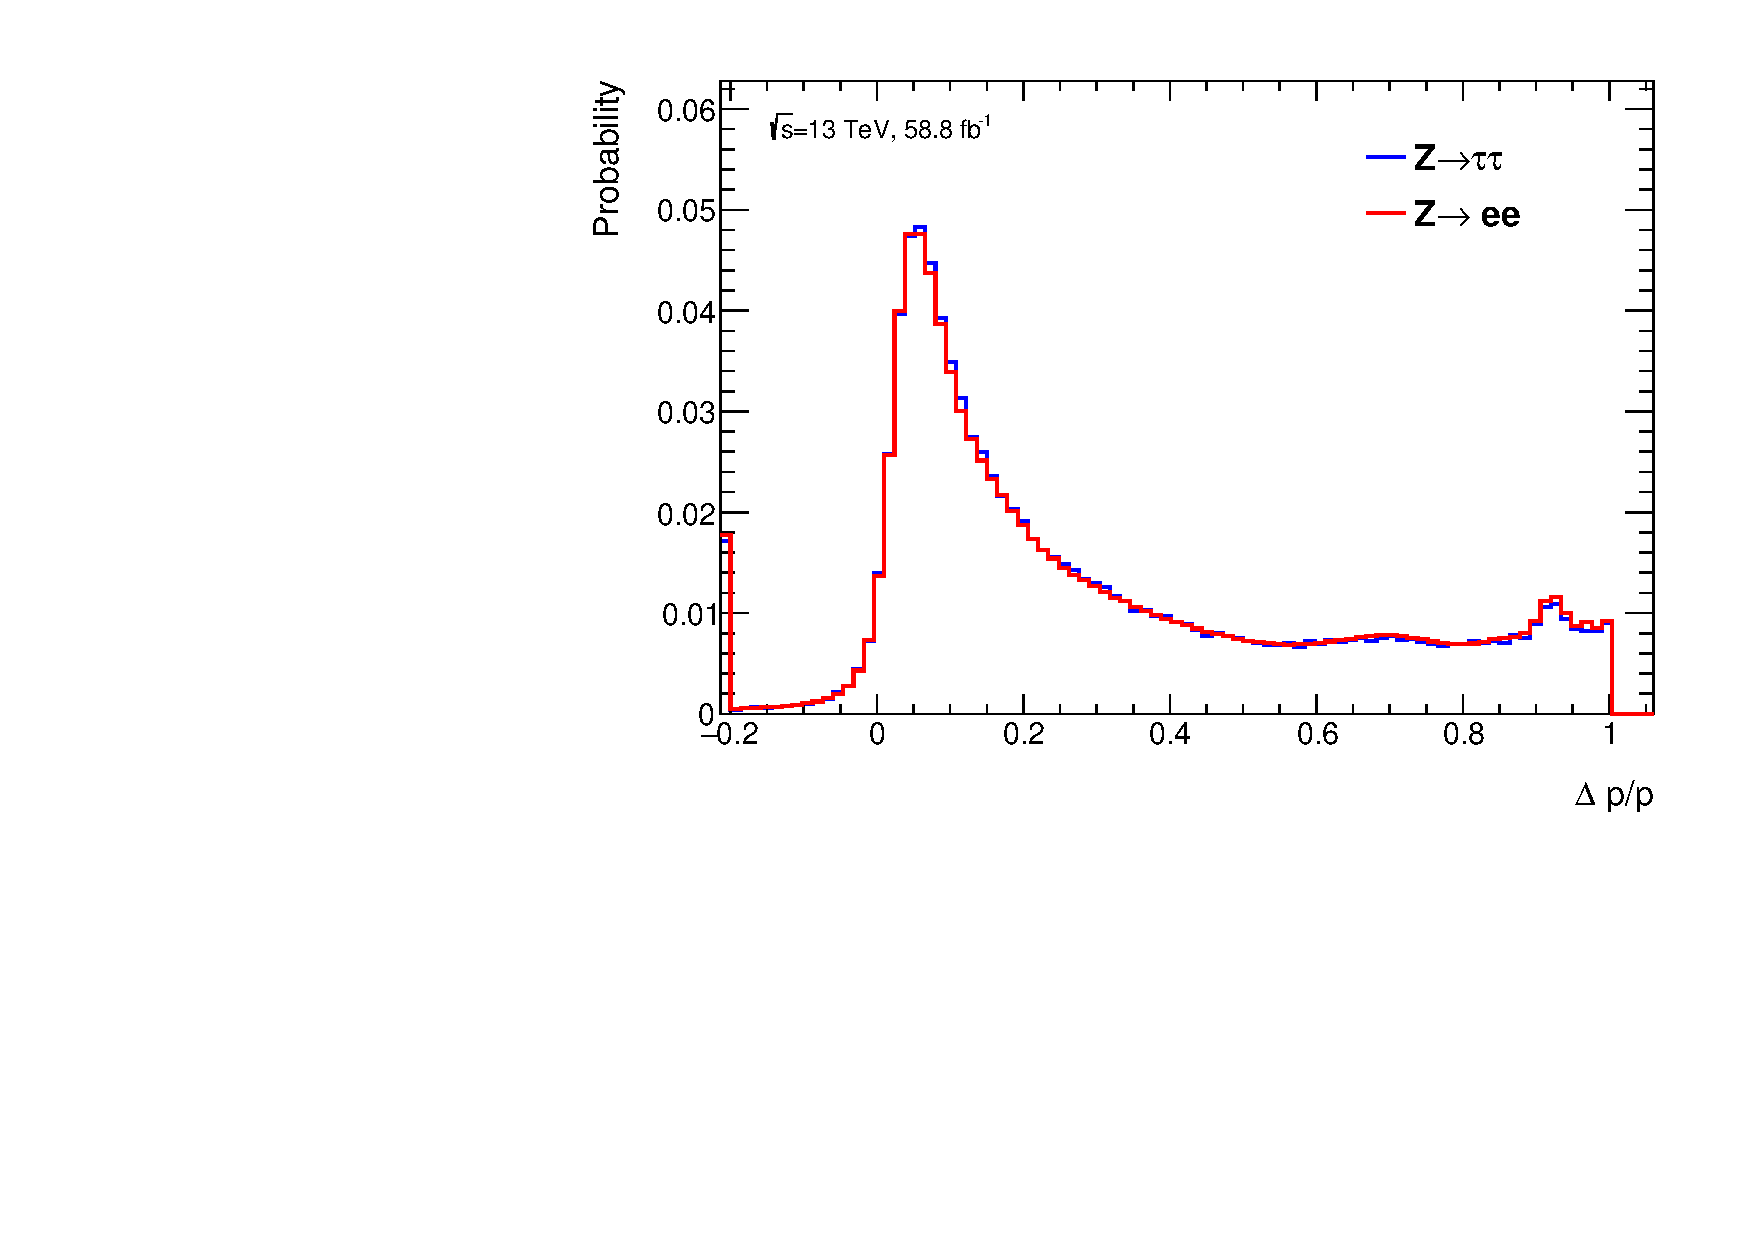
\includegraphics[width=\linewidth]{h_dPOverP_Ztautau_comparison.pdf}
      \caption{}
  \end{subfigure}
  \caption{Comparison of distributions for two calorimeter-based variables (a) and (b), between prompt electrons from $Z \rightarrow ee$ decays and $\tau_{e}$ electrons from $Z \rightarrow \tau\tau$ obtained in MC. The definition of these variables is detailed in Table~\ref{table:inputs}.}
  \label{fig:compare}
\end{figure}


\begin{figure}[htbp]
  \centering
  \includegraphics[width=0.7\textwidth]{h_d0Sig_Ztautau_comparison.pdf}
  \caption{Comparison of distributions for an impact parameter related variable between prompt electrons from $Z \rightarrow ee$ decays and $\tau_{e}$ electrons from $Z \rightarrow \tau\tau$ obtained in MC. The definition of this variables is detailed in Table~\ref{table:inputs}.}
  \label{fig:compare2}
\end{figure}
A similar situation arises with electrons from Heavy-Flavour decays: although generally treated as background for training purposes, some analyses may require keeping them or applying dedicated rejection techniques. In this context, the class definitions used in this work are optimised for the training of the DNN, but they may need to be reinterpreted depending on the specific analysis requirements.


\subsubsection{Inputs and preprocessing}
\label{inputs_preproc}
%Define which variables are used and why, as well as how we treat them before they're passed through the NN. Hablar obviamente de correction factors, fudging, problems with fudging, correlations and so on.
In order to feed the DNN with the features from the different classes of electron candidates, information left by these particles in almost all ATLAS subdetectors (except the MS) is used, as well as matching information between the tracking systems and energy deposits in the calorimeter. 
In Table~\ref{table:inputs}, all the variables used are listed, along with a brief definition for each of them.

As specified, there are some variables that are not used as input features for training the DNN, but are instead applied as simple rectangular cuts afterwards, in the optimisation step that will be detailed in the next section, since in some specific cases they could provide additional discrimination power. There are also other variables that, in addition to being used for training, are also employed for these rectangular cuts, such as $n_{\text{Si}}$ and $n_{\text{Pixel}}$.

As previously mentioned, the choice of input variables is not exactly the same as the one used to construct the LH discriminant~\cite{Aaboud:2657964}. First of all, the \et and $\eta$ of the electron candidates appear indirectly in the LH construction, since the PDFs are provided in different bins of these variables in order to account for the differences in the kinematic features of the candidates across the various regions of the phase space. Since replicating this binning strategy for the DNN would be computationally expensive, these variables have been instead included as inputs to provide the model with information about the phase space, although, as will be discussed, they are treated with special care. \clearpage

{\scriptsize
\begin{longtable}{p{2.3cm}p{7cm}p{1.5cm}p{1.5cm}}
  \caption{Input variables for electron identification DNN. Variables with ``C'' in usage are used to perform additional rectangular cuts when defining the DNN WPs. In the variables constructed using the second layer of the calorimeter, $3\times3$, $3\times5$, $3\times7$ and $7\times7$ cells refer to areas of $\Delta \eta \times \Delta \phi$ space in units of $0.025\times0.0245$. Description based on Ref.~\cite{dnn_paper}.}\\
  \toprule
  \textbf{Type} & \textbf{Description} & \textbf{Name} & \textbf{Usage} \\
  \midrule
  \endfirsthead
  \midrule
  \endhead
  Hadronic leakage & Ratio of $E_{\text{T}}$ in the first layer of the HCAL to $E_{\text{T}}$ of the EM cluster. & $R_{\text{had1}}$ & DNN \\
   & Ratio of $E_{\text{T}}$ in the HCAL to $E_{\text{T}}$ of the EM cluster. & $R_{\text{had}}$ & DNN \\
  \midrule
  Third layer of EM calorimeter & Ratio of the energy in the third layer to the total energy in the ECAL. & $f_3$ & DNN \\
  \midrule
  First layer of EM calorimeter & Lateral shower width in the second layer of the ECAL. & $w_{\eta2}$ & DNN \\
   & Ratio of the energy in $3{\times}3$ cells in the second layer of the ECAL over the energy in $7{\times}7$ cells centered at the electron cluster position. & $R_{\eta}$ & DNN \\
   & Ratio of the energy in $3{\times}7$ cells in the second layer of the ECAL over the energy in $7{\times}7$ cells centered at the electron cluster position. & $R_{\phi}$ & DNN \\
   & Shower width in the first layer of the ECAL. & $w_{\text{stot}}$ & DNN\\
   & Ratio of the energy difference between the maximum energy deposit and the energy deposit in a secondary maximum in the cluster to the sum of these energies in the first layer of the ECAL. & $E_{\text{ratio}}$ & DNN \\
   & Ratio of the energy in the first layer to the total energy in the ECAL. & $f_1$ & DNN \\
  \midrule
  Track  & Number of hits in the Pixel detector. & $n_{\text{Pixel}}$ & DNN + C \\
   & Extra hit required in the insertable BLayer. & \texttt{BLayer} & C \\
   & Total number of hits in the Pixel and SCT detectors. & $n_{\text{Si}}$ & DNN + C \\
   & Charged transverse impact parameter relative to the beam-line. & $q \times d_0$ & DNN \\
   & Electron weighted average charge over all associated SCT tracks. & q_{\text{SCT}} & DNN \\
   & Significance of transverse impact parameter defined as the ratio of $d_0$ to its uncertainty. & $|d_0/\sigma(d_0)|$ & DNN \\
   & Momentum lost by the track between the perigee and the last measurement point divided by the momentum at perigee. & $\Delta p/p$ & DNN \\
  \midrule
  TRT & LH probability based on transition radiation in the TRT. & \scriptsize{\texttt{TRT PID}} & DNN \\
  \midrule
  Track-cluster matching & $\Delta\eta$ between the cluster position in the first layer and the extrapolated track. & $\Delta\eta_1$ & DNN \\
   & $\Delta\phi$ between the cluster position in the second layer of the ECAL and the momentum-rescaled track. & $\Delta\phi_{\text{res}}$ & DNN \\
   & Ratio of the cluster energy to the track momentum. & $E/p$ & DNN\\
   & Transverse ene
   rgy of the electron measured by the calorimeter system. & $E_{\text{T}}$ & DNN \\
   & Absolute value of the pseudorapidity of the electron. & $|\eta|$ & DNN \\
  \midrule 
  Reconstruction & Output of an ambiguity resolution algorithm to distinguish objects reconstructed as both electrons and photons. & \scriptsize{\texttt{Amb-type}} & C \\
  \bottomrule
  \label{table:inputs}
\end{longtable}
}

Moreover, it has been already mentioned that the number of hits in the main track of our electron candidates is not only used for rectangular cuts, as done in the LH approach, but also as input variables in the training together with other variables like $E/p$ and $w_{\text{stot}}$. 

Most importantly, this strategy allows the usage of highly correlated variables, such as $R_{\text{had1}}$ and $R_{\text{had}}$, which capture at different levels the fraction of energy from the EM cluster that leaks into the hadronic calorimeter. In the LH construction, by definition, only one of these variables can be used, depending on the detector geometry region. In contrast, ML algorithms such as DNNs can greatly benefit from input feature correlations, especially in classification tasks where correlations differ across the various classes.

It is also important to highlight that two variables included in the list are not used in the LH approach nor in the previous version of this DNN~\cite{dnn_paper}. 

The first of these variables is the so-called \texttt{SCTWeightedCharge}, also denoted as $q_{\text{SCT}}$, which is defined as:
\begin{equation}
  q_{\text{SCT}} = q^{e}\sum_{\text{trk}}\left( q^{\text{trk}}N^{\text{trk}}_{\text{SCT}} \right)/\sum_{\text{trk}} N^{\text{trk}}_{\text{SCT}}
\end{equation}
where $q^{e}$ is the charge of the electron (as given by its primary track), $N^{\text{trk}}_{\text{SCT}}$ is the number of hits in the SCT for a given track associated to the electron, and $q^{\text{trk}}$ is the charge associated to that track. This variable can be interpreted as the electron charge weighted over all tracks associated with the electron, beyond the primary one. By construction, it takes a value of one if the electron has only one associated track. However, in cases where multiple tracks are associated to the same electron candidate, the value may differ from one, which is typically more likely when the candidate corresponds to a charge-flip electron.

The second variable is the so-called charged impact parameter, $q \times d_{0}$, which replaces the $d_{0}$ variable used previously.

The main interest of these two variables lies in their discriminating power for rejecting charge-flip electrons against prompt electrons candidates with correctly identified charge~\cite{carnelli}, property that can be observed in the the plots shown in Figure~\ref{fig:cf_plots}. This provides the DNN with an additional potential to identify this specific class of electrons. This feature will be discussed in more detail in Section~\ref{dnn:tuning}.

\begin{figure}[htbp]
  \centering
  \begin{subfigure}[b]{0.49\textwidth}
      \includegraphics[width=\textwidth]{images/selection_MultiClass_qd0_train.pdf}
      \caption{}
  \end{subfigure}
  \begin{subfigure}[b]{0.49\textwidth}
      \includegraphics[width=\textwidth]{images/selection_MultiClass_sctweightedcharge_train.pdf}
      \caption{}
  \end{subfigure}
  \caption{Distributions of the new variables, (a) $q \times d_{0}$ and (b) $q_{\text{SCT}}$, considered to improve the rejection of CF electrons from prompt electrons.}
  \label{fig:cf_plots}
\end{figure}

\paragraph{Shower-shape variables corrections} \mbox{}\\
\\
Shower-shape variables characterize the development of the EM shower produced by the electron candidates in the calorimeter.

In order for the DNN to be trained and to perform well when applied to real data, the distributions of the input variables for simulated electrons should resemble those of genuine electrons observed in data. However, due to imperfections in the detector modelling, the disagreement between MC simulations and data can be too large. % (especially for those variables involving calorimeter signal readouts. such as energy leakage due to undesired connections between LAr cells, commonly referred to as \textit{cross-talk}).

Corrections are applied to these shower-shape variables in order to improve their modelling of the real data. These corrections are based on individual affine transformations applied in bins of $E_{\text{T}}$ and $\eta$, such that the mean of the distribution being stretched and/or its width shifted, depending on the severity of the discrepancy.

The corrections are derived by comparing the distributions evaluated for \zee electron candidates extracted from data and MC simulations using the tag-and-probe technique. The transformation parameters are obtained by minimising the $\chi^2$ between the two distributions. More details can be found in Ref.~\cite{Aaboud:2657964}, but an example of the application of these corrections can be seen in Figure~\ref{fig:corrected} for the variables $f_{3}$ and $R_{\text{had}}$.


\begin{figure}[htbp]
  \centering
  \begin{subfigure}[b]{0.48\textwidth}
      \includegraphics[width=\textwidth]{id_datamcf3.png}
      \caption{}
  \end{subfigure}
  \hfill
  \begin{subfigure}[b]{0.48\textwidth}
      \includegraphics[width=\textwidth]{id_datamcrhad.png}
      \caption{}
  \end{subfigure}
  \hfill
  \caption{Comparison of (a)$f_{3}$ and (b)$R_{\text{had}}$ shower-shape distributions for data and MC electrons with and without corrections applied, within certain $E_{\text{T}}$ and $\eta$ bins: $30 < E_{\text{T}} < 40$~GeV and $0.8<|\eta|<1.15$~\cite{Aaboud:2657964}.}
  \label{fig:corrected}
\end{figure}

It can be observed that, in the case of $f_3$, the simulated values of this variable are centred around a mean value that is slightly shifted with respect to the real data distribution. Therefore, in this case, a small shift in the mean of the distribution would be sufficient. 
For $R_{\text{had}}$, however, it is also evident that in order to match the data values, it is necessary not only to shift the distribution but also to broaden it slightly around the mean value, applying a correction to the width as well.

%SHIFT&STRETCH Y QUE HAY OTRO QUE SE USO QUE NO VALE PARA DNN POR LAS CORRELACIONES Y PONER PLOTS DE CORRELACIONES Y DECIR QUE SE CONSERVAN GUAY ;)
This correction method, often referred to as \textit{fudging} in this context, is known as the \textit{Shift}$\&$\textit{Stretch} approach. Other strategies exist to address discrepancies between data and MC simulations, such as the \textit{Gaussian Smearing} approach, which assumes that the noise-like imperfections introduced by the calorimeter can be incorporated into MC simulations through Gaussian approximations~\cite{Puddefoot:2797826}.

This \textit{Gaussian Smearing} approach was used to correct the PDFs employed in the construction of the LH discriminant using rel.22 Run-2 datasets. However, it cannot be applied to the DNN input variables, since these Gaussian corrections introduce artificial correlations in the input distributions, which degrade the performance of the DNN. Unlike the LH method, which is designed to be robust against such effects, DNNs rely on the preservation of meaningful correlations between features.

The \textit{Shift}$\&$\textit{Stretch} method, on the other hand, applies simple affine transformations that better preserve these correlations. This can be seen in Figure~\ref{fig:correlations}, where the correlation matrices between input variables are shown for MC simulations before and after corrections, and for collision data.

\begin{figure}[h]
  \centering
  \begin{subfigure}[b]{0.49\textwidth}
      \centering
      \includegraphics[width=\textwidth]{correlation_matrix_nofudge_eta_gt241_f1.png}
      \caption{MC without corrections}
      \label{fig:corr_nominal}
  \end{subfigure}
  \hfill
  \begin{subfigure}[b]{0.49\textwidth}
      \centering
      \includegraphics[width=\textwidth]{correlation_matrix_data18_eta_gt241_f1.png}
      \caption{Data}
      \label{fig:corr_data}
  \end{subfigure}
  \\
  \vspace{0.4cm}
  \begin{subfigure}[b]{0.49\textwidth}
      \centering
      \includegraphics[width=\textwidth]{correlation_matrix_newtool_eta_gt241_f1.png}
      \caption{MC with Gaussian Smearing}
      \label{fig:corr_smearing}
  \end{subfigure}
  \hfill
  \begin{subfigure}[b]{0.49\textwidth}
      \centering
      \includegraphics[width=\textwidth]{correlation_matrix_oldtool_newderivedFFs_eta_gt241_f1.png}
      \caption{MC with Shift\&Stretch}
      \label{fig:corr_shiftstretch}
  \end{subfigure}
  \caption{Comparison of input variable correlations for different correction strategies. Only electrons from the end-cap region ($|\eta|>2.41$) and with $f_{1}=0$ are selected since are more representative of this discrepancy between approaches.}
  \label{fig:correlations}
\end{figure}

\paragraph{Preprocessing} \mbox{}\\
\\
As different physical processes have been used to populate the various electron candidate classes, the $E_{\text{T}}$ distribution can vary significantly among them. For instance, most prompt electrons from $Z \to e^{+}e^{-}$ decays will have $E_{\text{T}} \approx 45$~GeV, corresponding to half of the $Z$-boson mass, as can be seen in Figure~\ref{fig:et_eta_selection}. This could introduce significant biases and degrade the DNN’s performance, as discussed in Section~\ref{dnn:preprocessing}.
To prevent the network from distinguishing classes based solely on $E_{\text{T}}$ and $\eta$, these input distributions need to be harmonised across all six classes. This is achieved through a combination of downsampling and reweighting.

\begin{figure}[h]
  \centering
  \begin{subfigure}[b]{0.6\textwidth}
      \centering
      \includegraphics[width=\textwidth]{selection_MultiClass_Et_train.pdf}
      \caption{}
      \label{fig:et_selection}
  \end{subfigure}
  \begin{subfigure}[b]{0.6\textwidth}
      \centering
      \includegraphics[width=\textwidth]{selection_MultiClass_Eta_train.pdf}
      \caption{}
      \label{fig:eta_selection}
  \end{subfigure}
  \caption{Distributions of (a) $E_{\text{T}}$ and (b) $\eta$ at electron selection level.}
  \label{fig:et_eta_selection}
\end{figure}

First, to limit the statistical imbalance, the prompt electron sample is downsampled. Prompt candidates are randomly removed in $E_{\text{T}}$ bins so that, within each bin, their number does not exceed five times the number of background candidates. This effectively reduces the prominent peak at 45~GeV, as illustrated in Figure~\ref{fig:et_downsampled}. Due to limited statistics, no downsampling is applied to the charge-flip class, even though a similar peak is present.

\begin{figure}[h]
  \centering
  \includegraphics[width=0.6\textwidth]{downsampled_MultiClass_Et_train.pdf}
  \caption{Distribution of $E_{\text{T}}$ after applying downsampling.}
  \label{fig:et_downsampled}
\end{figure}

Once downsampling is applied, weights are derived to reweight the $E_{\text{T}}$ and $\eta$ distributions independently for each class. These weights are then combined by multiplying the two, assuming no strong correlation between $E_{\text{T}}$ and $\eta$. After reweighting, all distributions are normalised so that the sum of weight per class remains constant. The resulting harmonised distributions for $E_{\text{T}}$ and $\eta$ are shown in Figure~\ref{fig:et_eta_reweighted}.

The $\eta$ reweighting aims for a flat distribution, while for $E_{\text{T}}$, a flat region until 15~GeV is targeted, followed by falling slope resembling the shape of the Light-Flavour hadron class. This approach reduces the bias efficiently while preserving classification performance. Some residual discrepancies may remain due to small final correlations between $E_{\text{T}}$ and $\eta$, especially for the charge-flip class. While a 2D reweighting could mitigate this, it is avoided due to limited statistics at high $E_{\text{T}}$.

\begin{figure}[htbp]
  \centering
  \begin{subfigure}[b]{0.6\textwidth}
      \centering
      \includegraphics[width=\textwidth]{weighted_MultiClass_Et_train.pdf}
      \caption{}
      \label{fig:et_reweighted}
  \end{subfigure}
  \begin{subfigure}[b]{0.6\textwidth}
      \centering
      \includegraphics[width=\textwidth]{weighted_MultiClass_Eta_train.pdf}
      \caption{}
      \label{fig:eta_reweighted}
  \end{subfigure}
  \caption{Distributions of (a) $E_{\text{T}}$ and (b) $\eta$ after applying downsampling and kinematic reweighting.}
  \label{fig:et_eta_reweighted}
\end{figure}

Finally, to equalise the total statistical weight across classes, an additional scaling factor is applied per class after reweighting. This factor ensures that all classes contribute equally in terms of weight, while keeping the global sum of weights unchanged. An example of this normalization is shown in the case of the $E_{\text{T}}$ distribution in Figure~\ref{fig:et_classWeighted}.

\begin{figure}[htbp]
  \centering
  \includegraphics[width=0.6\textwidth]{classWeighted_MultiClass_Et_train.pdf}
  \caption{Distribution of $E_{\text{T}}$ after applying class weighting, making all classes equiprobable.}
  \label{fig:et_classWeighted}
\end{figure}


% === Figure A: rows 1–3 (6 panels) ===
\begin{figure}[htbp]
  \centering

  % Row 1
  \begin{subfigure}[b]{0.49\textwidth}
    \centering
    \includegraphics[width=\linewidth]{normalized_weighted_distributions/weighted_Multiclass_rhad1_train.pdf}
    \caption{$R_{\text{had1}}$}
    \label{fig:input1}
  \end{subfigure}\hfill
  \begin{subfigure}[b]{0.49\textwidth}
    \centering
    \includegraphics[width=\linewidth]{normalized_weighted_distributions/weighted_Multiclass_rhad_train.pdf}
    \caption{$R_{\text{had}}$}
    \label{fig:input2}
  \end{subfigure}

  \vspace{0.45cm}

  % Row 2
  \begin{subfigure}[b]{0.49\textwidth}
    \centering
    \includegraphics[width=\linewidth]{normalized_weighted_distributions/weighted_Multiclass_f3_train.pdf}
    \caption{$f_3$}
    \label{fig:input3}
  \end{subfigure}\hfill
  \begin{subfigure}[b]{0.49\textwidth}
    \centering
    \includegraphics[width=\linewidth]{normalized_weighted_distributions/weighted_Multiclass_weta2_train.pdf}
    \caption{$w_{\eta2}$}
    \label{fig:input4}
  \end{subfigure}

  \vspace{0.45cm}

  % Row 3
  \begin{subfigure}[b]{0.49\textwidth}
    \centering
    \includegraphics[width=\linewidth]{normalized_weighted_distributions/weighted_Multiclass_reta_train.pdf}
    \caption{$R_{\eta}$}
    \label{fig:input5}
  \end{subfigure}\hfill
  \begin{subfigure}[b]{0.49\textwidth}
    \centering
    \includegraphics[width=\linewidth]{normalized_weighted_distributions/weighted_Multiclass_rphi_train.pdf}
    \caption{$R_{\phi}$}
    \label{fig:input6}
  \end{subfigure}

  \caption{Distributions of all the input variables used for DNN training, after preprocessing and reweighting procedures. Only the training subset of the simulated electrons is used to produce these plots.}
  \label{fig:dnn_inputs_distributions_A}
\end{figure}

% === Figure B: rows 4–6 (6 panels) ===
\begin{figure}[htbp]
  \centering

  % Row 4
  \begin{subfigure}[b]{0.49\textwidth}
    \centering
    \includegraphics[width=\linewidth]{normalized_weighted_distributions/weighted_Multiclass_wtots1_train.pdf}
    \caption{$w_{stot}$}
    \label{fig:input7}
  \end{subfigure}\hfill
  \begin{subfigure}[b]{0.49\textwidth}
    \centering
    \includegraphics[width=\linewidth]{normalized_weighted_distributions/weighted_Multiclass_eratio_train.pdf}
    \caption{$E_{\text{ratio}}$}
    \label{fig:input8}
  \end{subfigure}

  \vspace{0.45cm}

  % Row 5
  \begin{subfigure}[b]{0.49\textwidth}
    \centering
    \includegraphics[width=\linewidth]{normalized_weighted_distributions/weighted_Multiclass_f1_train.pdf}
    \caption{$f_1$}
    \label{fig:input9}
  \end{subfigure}\hfill
  \begin{subfigure}[b]{0.49\textwidth}
    \centering
    \includegraphics[width=\linewidth]{normalized_weighted_distributions/weighted_Multiclass_npixel_train.pdf}
    \caption{$n_{\text{Pixel}}$}
    \label{fig:input11}
  \end{subfigure}

  \vspace{0.45cm}

  % Row 6
  \begin{subfigure}[b]{0.49\textwidth}
    \centering
    \includegraphics[width=\linewidth]{normalized_weighted_distributions/weighted_Multiclass_nsilicon_train.pdf}
    \caption{$n_{\text{Si}}$}
    \label{fig:input12}
  \end{subfigure}\hfill
  \begin{subfigure}[b]{0.49\textwidth}
    \centering
    \includegraphics[width=\linewidth]{normalized_weighted_distributions/weighted_Multiclass_TRTPID_train.pdf}
    \caption{TRT PID}
    \label{fig:input18}
  \end{subfigure}

  \caption{Distributions of all the input variables used for DNN training, after preprocessing and reweighting procedures. Only the training subset of the simulated electrons is used to produce these plots.}
  \label{fig:dnn_inputs_distributions_B}
\end{figure}

% === Figure C: rows 7–8 (4 panels) ===
\begin{figure}[htbp]
  \centering

  % Row 7
  \begin{subfigure}[b]{0.49\textwidth}
    \centering
    \includegraphics[width=\linewidth]{normalized_weighted_distributions/weighted_Multiclass_d0sig_train.pdf}
    \caption{$|d_0/\sigma(d_0)|$}
    \label{fig:input16}
  \end{subfigure}\hfill
  \begin{subfigure}[b]{0.49\textwidth}
    \centering
    \includegraphics[width=\linewidth]{normalized_weighted_distributions/weighted_Multiclass_qd0_train.pdf}
    \caption{$q \times d_0$}
    \label{fig:input14}
  \end{subfigure}

  \vspace{0.45cm}

  % Row 8
  \begin{subfigure}[b]{0.49\textwidth}
    \centering
    \includegraphics[width=\linewidth]{normalized_weighted_distributions/weighted_Multiclass_sctweightedcharge_train.pdf}
    \caption{$q_{\text{SCT}}$}
    \label{fig:input15}
  \end{subfigure}\hfill
  \begin{subfigure}[b]{0.49\textwidth}
    \centering
    \includegraphics[width=\linewidth]{normalized_weighted_distributions/weighted_Multiclass_dPoverP_train.pdf}
    \caption{$\Delta p/p$}
    \label{fig:input17}
  \end{subfigure}

  \caption{Distributions of all the input variables used for DNN training, after preprocessing and reweighting procedures. Only the training subset of the simulated electrons is used to produce these plots.}
  \label{fig:dnn_inputs_distributions_C}
\end{figure}

The distributions of all input variables after the application of these modifications (except the class-reweighting) can be found in Figures~\ref{fig:dnn_inputs_distributions_A}-\ref{fig:dnn_inputs_distributions_C}. However, there is still one last step before passing all the inputs distributions through the DNN training, which is the transformation to uniform distributions between zero and one, using empirical quantiles as explained in Section~\ref{dnn:preprocessing}. This action facilitates the training of the neural network and speeds up the different steps in the optimization.
Figure~\ref{fig:transformed} illustrates the impact of this transformation on the $R_{\text{had}}$ variable, taken from Ref.~\cite{dnn_paper}. The plot displays the full distribution together with the individual contributions from prompt electrons and Light-Flavour hadrons. After applying the transformation, the overall distribution becomes uniform within the $[0,1]$ interval.

\begin{figure}[htbp]
  \centering
  \begin{subfigure}[b]{0.49\textwidth}
      \includegraphics[width=\textwidth]{rhad_original.png}
      \caption{}
  \end{subfigure}
  \hfill
  \begin{subfigure}[b]{0.49\textwidth}
      \includegraphics[width=\textwidth]{rhad_transformed.png}
      \caption{}
  \end{subfigure}
  \hfill
  \caption{Distribution of $R_{\text{had}}$ for all candidates, prompt electrons, and Light-Flavour hadrons, shown (a) before and (b) after applying the QuantileTransformer. Distributions include downsampling and reweighting and only two classes are displayed for clarity. In these studies presented in Ref.~\cite{dnn_paper}, an additional $Z\gamma$ input was used.}
  \label{fig:transformed}
\end{figure}

\subsubsection{Training procedure}

In this work, a DNN with a total of five hidden layers has been employed, each containing 256 nodes. In these hidden layers, the Leaky ReLU activation function is applied to introduce non-linearity, as detailed in Section~\ref{sec:dnn_general}, and batch normalization is also implemented.  
This algorithm performs a multinomial classification, producing as output a total of six scores, one for prompt electrons ($p_{El}$) and five for each of the background classes ($p_{CF}$, $p_{HF}$, $p_{PC}$, $p_{LFEg}$ and $p_{LFH}$). In the final output layer, the Softmax activation function is applied.  
A schematic diagram of our DNN architecture is shown in Figure~\ref{dnn_sketch}.

\begin{figure}[htbp]
  \centering
  \includegraphics[width=0.8\textwidth]{dnn_sketch.png}
  \caption{Overview diagram of the architecture of the electron identification DNN. It is shown the optimised number of layers and nodes used in the final version. Taken from Ref.~\cite{dnn_paper}.}
  \label{dnn_sketch}
\end{figure}

This algorithm was implemented and trained using the \texttt{Python} \texttt{tensorflow} library~\cite{tensorflow2015}, version~2.4. As previously mentioned, the $Adam$ optimizer was used in the training procedure. Regarding the remaining hyperparameters of the neural network, different configurations were tested, and the one showing the best performance was selected.  
The final training is performed over a total of 100 epochs, retaining as the final result the iteration that yields the lowest loss on the validation dataset.

\subsubsection{Electron classification}

The decision to employ a multinomial classification as the output of our DNN allows for distinguishing between the different background classes that typically populate our real collision data. Beyond kinematics, the most relevant input variables also differ across classes, for instance reflecting the distinct characteristics of the calorimeter showers that they produce in the detector. As an illustration, electron candidates originating from $b$- or $c$-hadrons tend to deposit more energy in the innermost layers than prompt electrons, as can be seen in Figure~\ref{fig:input2}.

Nevertheless, for the purpose of identifying signal electrons over the rest of the background candidates, a binomial discrimination must ultimately be performed when defining our working points as a function of efficiencies.  
For this, the following binomial discriminant is defined, simply combining the output given by the DNN:

\begin{equation}
  \small
  %\footnotesize
  \mathcal{D}_{el} = \ln\left(\frac{f_{El}p_{El} + (1-f_{El})p_{CF}}{f_{PC}p_{PC}+f_{HF}p_{HF}+f_{LFEg}p_{LFEg}+(1-f_{PC}-f_{HF}-f_{LFEg})p_{LFH}}\right)
\label{eq:dnn_discriminant}
\end{equation}
where $p_{X}$ are the scores provided by the DNN for each class, and $f_{X}$ are tunable parameters or weights, referred to as \textit{fractions}, which control the relative importance of the different classes in the discriminant.  
This discriminant separates electron candidates considered as signal, in a generic electron identification problem, which in this case are prompt and Charge-Flip electrons (therefore placed in the numerator), from the remaining background electrons in the denominator.

As mentioned, the fractions $f_{X}$ are tunable, and to simplify the procedure it is imposed that their sum equals unity in both numerator and denominator. Depending on the physics analysis under study and the composition of its final states, one background class may be more relevant than another, and this is fully configurable.

Ideally, the determination of these fractions would be performed directly from real data, just as is done for the LH during training. However, obtaining sufficiently pure and unbiased control regions from data is a highly challenging task.
For this reason, in generic electron identification studies presented in this thesis, the fractions are tuned and the performance of the DNN is evaluated using the test dataset obtained from the simulated input samples. 

The tuning of these fractions, the evaluation of the algorithm’s performance, and the subsequent derivation of working points are performed in bins of $|\eta|$ and/or $E_{\text{T}}$, to account for variations in the spectra of the different electron candidate classes, without any downsampling or reweighting applied. 
As a figure of merit for estimating the performance of our algorithm and comparing it to the LH, ROC curves are used, already described in Chapter~\ref{chap:machine_learning}.

The calculation of the $f_{X}$ is parametrized only in different $|\eta|$ bins. The same fractions are applied across the full $E_{\text{T}}$ range to obtain a smooth and continuous discriminant over the entire energy spectrum.
The optimal $f_{X}$ values are obtained by maximising the Area Under the Curve (AUC) of the ROC associated with the $\mathcal{D}_{el}$ discriminant, allowing all fractions to float. The optimisation is performed in the range between $70\%$ and $95\%$ signal efficiency, which corresponds to the typical operating window of electron identification working points. The $|\eta|$ bins employed here are broader than those used later when defining the DNN working points, which apply cuts on the discriminant as explained in Section~\ref{dnn:tuning}.
Table~\ref{tune:binning} lists the $|\eta|$ and $E_{\text{T}}$ bin boundaries used in each case.

\begin{table}[htbp]
  \centering
  \caption{Bin edges used for the discriminant cuts and for the $f_X$ optimisation.}
  \footnotesize
  \setlength{\tabcolsep}{5pt}
  \renewcommand{\arraystretch}{1.1}

  % Primera tabla: |eta|
  \begin{subtable}[t]{\linewidth}
    \centering
    \subcaption{Bin boundaries in $|\eta|$}
    \vspace{2pt}
    \begin{tabular}{@{}ll@{}}
      \toprule
      \textbf{Use} & \textbf{Edges} \\
      \midrule
      Discriminant cuts &
      $0.0,\ 0.1,\ 0.6,\ 0.8,\ 1.15,\ 1.37,\ 1.52,\ 1.81,\ 2.01,\ 2.37,\ 2.47$ \\
      $f_X$ optimisation &
      $0.0,\ 0.8,\ 1.37,\ 1.52,\ 2.01,\ 2.47$ \\
      \bottomrule
    \end{tabular}
  \end{subtable}

  \vspace{0.4cm} % separación entre tablas

  % Segunda tabla: ET
  \begin{subtable}[t]{\linewidth}
    \centering
    \subcaption{Bin boundaries in $E_{\text{T}}$ [GeV]}
    \vspace{2pt}
    \begin{tabular}{@{}ll@{}}
      \toprule
      \textbf{Use} & \textbf{Edges} \\
      \midrule
      Discriminant cuts &
      $4,\ 7,\ 10,\ 15,\ 20,\ 25,\ 30,\ 35,\ 40,\ 45,\ \infty$ \\
      \bottomrule
    \end{tabular}
  \end{subtable}
  \label{tune:binning}
\end{table}

As previously mentioned, the $f_{X}$ values obtained in these bins from the test sample are considered optimal for this study. However, since the dataset composition may differ in other analyses, these values can be adjusted accordingly.
The relative contribution of each background electron class in the test sample used for the fractions optimization can be found in Table~\ref{tab:relative_contribution}, both inclusively and for the specific kinematic bin under study $(E_{\text{T}},|\eta|)$.
\begin{table}[htbp]
  \centering
  \caption{Fractions and statistical errors for all candidates and for the selected kinematic bin.}
  \label{tab:relative_contribution}
  \begingroup
  \scriptsize
  \setlength{\tabcolsep}{3pt}
  \renewcommand{\arraystretch}{1.05}

  % anchos de columnas numéricas (ajusta si quieres)
  \newcommand{\FracW}{18mm}
  \newcommand{\ErrW}{15mm}
  \newcommand{\ClassW}{25mm}

  \begin{subtable}[t]{0.49\linewidth}
    \centering
    \subcaption{Inclusive}
    \vspace{2pt}
    \begin{tabular}{@{}%
      >{\raggedright\arraybackslash}p{\ClassW}%
      >{\raggedleft\arraybackslash}p{\FracW}%
      >{\raggedleft\arraybackslash}p{\ErrW}%
      @{}}
      \toprule
      \textbf{Class} & \textbf{Fraction [\%]} & \textbf{Stat. error} \\
      \midrule
      Photon Conv.       & 0.3251  & $\pm$ 0.0010 \\
      Heavy-Flavour            & 7.444   & $\pm$ 0.002  \\
      Light-Flavour e/$\gamma$ & 17.731  & $\pm$ 0.003  \\
      Light-Flavour had.   & 71.796  & $\pm$ 0.007  \\
      \bottomrule
    \end{tabular}
  \end{subtable}\hfill
  \begin{subtable}[t]{0.49\linewidth}
    \centering
    \subcaption{\scriptsize $15<E_{\text{T}}\leq 20~\mathrm{GeV}$, $0.0<|\eta|\leq 0.8$}
    \vspace{2pt}
    \begin{tabular}{@{}%
      >{\raggedright\arraybackslash}p{\ClassW}%
      >{\raggedleft\arraybackslash}p{\FracW}%
      >{\raggedleft\arraybackslash}p{\ErrW}%
      @{}}
      \toprule
      \textbf{Class} & \textbf{Fraction [\%]} & \textbf{Stat. error} \\
      \midrule
      Photon Conv.       & 0.611   & $\pm$ 0.004 \\
      Heavy-Flavour            & 19.658  & $\pm$ 0.024 \\
      Light-Flavour e/$\gamma$ & 11.946 & $\pm$ 0.019 \\
      Light-Flavour had.    & 66.63  & $\pm$ 0.05 \\
      \bottomrule
    \end{tabular}
  \end{subtable}

  \endgroup
\end{table}

With the $ \mathcal{D}_{el} $ discriminant now completely determined by the fractions, Figure~\ref{fig:dnn_final_disc_ab} shows its distribution evaluated for the different electron candidate classes, for a specific $|\eta|$ and $E_{\text{T}}$ bin.
% Figura 1: paneles (a) y (b)
\begin{figure}[htbp]
  \centering
  \begin{subfigure}[t]{0.48\linewidth}
    \centering
    \includegraphics[width=\linewidth]{discriminant_plots/panel_a.pdf}
    \caption{}
    \label{fig:dnnDisc_a}
  \end{subfigure}\hfill
  \begin{subfigure}[t]{0.48\linewidth}
    \centering
    \includegraphics[width=\linewidth]{discriminant_plots/panel_b.pdf}
    \caption{}
    \label{fig:dnnDisc_b}
  \end{subfigure}

  \caption{Signal discriminant $D_{\mathrm{el}}$ of the DNN shown for (a) prompt electrons,
  Charge-Flip electrons, photon conversions, and electrons from Heavy-Flavour decays; and
  (b) prompt electrons, $e/\gamma$ objects from Light-Flavour decays, and Light-Flavour hadrons.
  Electron candidates satisfy $15<E_{\text{T}}\leq 20~\mathrm{GeV}$ and $0.0<|\eta|\leq 0.8$.}
  \label{fig:dnn_final_disc_ab}
\end{figure}

% Figura 2: panel (c)
\begin{figure}[htbp]
  \centering
  \begin{subfigure}[t]{0.60\linewidth}
    \centering
    \includegraphics[width=\linewidth]{discriminant_plots/panel_c.pdf}
    \label{fig:dnnDisc_c}
  \end{subfigure}

  \caption{Signal discriminant $D_{\mathrm{el}}$ of the DNN shown for prompt electrons versus
  the combined background (all classes except prompt and Charge-Flip).
  Electron candidates satisfy $15<E_{\text{T}}\leq 20~\mathrm{GeV}$ and $0.0<|\eta|\leq 0.8$.}
  \label{fig:dnn_final_disc_c}
\end{figure}



In Figures~\ref{fig:dnn_final_disc_ab} and~\ref{fig:dnn_final_disc_c}, it can be observed that both signal electron classes, prompt and Charge-Flip, reach higher discriminant values, showing a more or less pronounced peak compared to the other background classes. Prompt electrons present a more distinctive distribution than Charge-Flip electrons, although in both cases there is a considerable population of Heavy-Flavour and Photon-Conversion background candidates toward the higher end of the range. However, these background distributions also tend to peak at lower discriminant values, which is equally important for achieving high identification efficiencies when defining thresholds.

It is worth noting that Heavy-Flavour electrons tend to populate a wide range of discriminant values compared to signal electrons, and in some cases even overlap with Photon-Conversion electrons. This can be explained by the fact that they originate from the decay of heavy quarks ($b$- and $c$-hadrons). If these hadrons had a shorter lifetime, their signatures and detector energy deposits would be more similar to those of prompt electrons, or even electrons from converted photons, which themselves can also be prompt. Part of this overlap is in fact reduced by the application of the rectangular cuts discussed previously.

In contrast, as seen in Figure~\ref{fig:dnnDisc_b}, the distributions of the Light-Flavour classes differ clearly from those of prompt electrons, which is highly advantageous and demonstrates the potential of our algorithm to reject these classes.

\subsubsection{Identification Performance}

Since the rejection power is expected to vary substantially across the different background classes, Receiver Operating Characteristic (ROC) curves are presented both individually for each background class and inclusively for all backgrounds combined. Due to their special status, charge-flip electrons are excluded from both signal and background definitions in the main performance evaluation.

Figure~\ref{fig:roc_allblkg} shows the ROC curves obtained with MC data for prompt electrons against electrons from all background classes, and in Figure~\ref{fig:roc_mainbkg} the ROCs curves against each background class individually are also shown. The signal definition always includes only prompt electrons, while the LH working points (Loose, Medium, Tight) are represented by single points, located at progressively lower signal efficiencies: Loose around $\varepsilon_{\rm sig} = 0.85$, Medium around $\varepsilon_{\rm sig} =0.75$, and Tight around $\varepsilon_{\rm sig} =0.65$.

Unlike the LH, the DNN curves shown do not include any additional rectangular cuts~\footnote{These rectangular cuts comprise the requirements on the number of hits in the pixel and silicon detectors, as well as an additional cut on the insertable B-Layer or a requirement on the ambiguity type, which are listed in Table~\ref{tab:wp_rectangular_cuts}.}, and therefore correspond to a slightly more relaxed selection, as the one used in the DNN training (at least 7 hits in the silicon detector and one pixel hit).

Quantitatively, at the LH~Loose WP, the DNN achieves a background rejection about two times higher than LH when considering all background classes combined. For Heavy-Flavour decays, the improvement at this efficiency is more evident, with a factor close to $2.2$, whereas for Light-Flavour $e/\gamma$ and undecayed hadrons the rejection also increases, by factors of about $4$ and $5$, respectively. Photon conversions show a moderate enhancement, with the DNN reaching a rejection about two times larger than LH. For Charge-Flip electrons, the improvement is striking, with the DNN achieving a rejection almost $8$ times higher than LH in this $\eta$ region.

Figure~\ref{fig:roc_cf} includes the ROC curve calculated for the rejection of Charge-Flip versus prompt electrons, shown merely to illustrate the capability of the DNN to separate both signal electron classes. In this case, a modified discriminant is used, where the Charge-Flip term is moved to the denominator in Eq.~\ref{eq:dnn_discriminant}:
\begin{equation}
  %\small
  \footnotesize
  \mathcal{D}_{el} = \ln\left(\frac{p_{El}}{f_{CF}p_{CF} + f_{PC}p_{PC}+f_{HF}p_{HF}+f_{LFEg}p_{LFEg}+(1-f_{CF}_f_{PC}-f_{HF}-f_{LFEg})p_{LFH}}\right)
\end{equation}
In any case, since the number of prompt electrons largely exceeds that of Charge-Flip electrons in any realistic selection, including Charge-Flip candidates within the signal definition would have a negligible impact on the overall signal efficiency.

In summary, the DNN consistently outperforms the LH in all background categories, with the most substantial benefits in rejecting backgrounds that exhibit distinctive calorimeter and tracking signatures, and smaller but still relevant gains for more signal-like sources such as Heavy-Flavour decays.

The most notable gains are expected for Light-Flavour hadrons, Light-Flavour $e/\gamma$, and Charge-Flip electrons, the latter benefiting greatly from the new variables added to the DNN, providing a significantly enhanced rejection across the full efficiency range. For Heavy-Flavour electrons, the smaller improvement reflects their closer resemblance to prompt electrons. Photon conversions also benefit moderately from the DNN, as their rejection is already relatively high with LH.


\begin{figure}[h]
  \centering
  \includegraphics[width=0.7\linewidth]{ROC/15_20_0p0_0p8/binnedROCCurve_et15_20_eta0.0_0.8.pdf}
  \caption{Background rejection versus signal efficiency (ROC curves) for prompt electrons against all background classes combined in a representative $(E_{\text{T}}, |\eta|)$ bin, and the statistical uncertainty of the background rejection is shown as a band.}
  \label{fig:roc_allblkg}
\end{figure}

% --- Primera figura ---
\begin{figure}[h]
  \centering
  % ---- Fila 1 ----
  \begin{subfigure}[t]{0.5\linewidth}
    \centering
    \includegraphics[width=\linewidth]{ROC/15_20_0p0_0p8/binnedROCCurvePhotonConv_et15_20_eta0.0_0.8.pdf}
    \caption{}
    \label{fig:roc_pc}
  \end{subfigure}\hfill
  \begin{subfigure}[t]{0.5\linewidth}
    \centering
    \includegraphics[width=\linewidth]{ROC/15_20_0p0_0p8/binnedROCCurveHeavyFlavor_et15_20_eta0.0_0.8.pdf}
    \caption{}
    \label{fig:roc_hf}
  \end{subfigure}

  \vspace{0.35cm}

  % ---- Fila 2 ----
  \begin{subfigure}[t]{0.5\linewidth}
    \centering
    \includegraphics[width=\linewidth]{ROC/15_20_0p0_0p8/binnedROCCurveLFEgamma_et15_20_eta0.0_0.8.pdf}
    \caption{}
    \label{fig:roc_lfeg}
  \end{subfigure}\hfill
  \begin{subfigure}[t]{0.5\linewidth}
    \centering
    \includegraphics[width=\linewidth]{ROC/15_20_0p0_0p8/binnedROCCurveLFHadron_et15_20_eta0.0_0.8.pdf}
    \caption{}
    \label{fig:roc_lfh}
  \end{subfigure}

  \caption{Background rejection versus signal efficiency (ROC curves) for prompt electrons against:
  (a) all background classes combined,
  (a) electrons from Heavy-Flavour decays,
  (b) $e/\gamma$ from Light-Flavour decays,
  (c) Light-Flavour hadrons,
  and (e) photon conversions.
  Curves are shown for a representative $(E_{\text{T}}, |\eta|)$ bin, and the statistical uncertainties of the each background rejection are shown as bands.}
  \label{fig:roc_mainbkg}
\end{figure}


% --- Segunda figura ---
\begin{figure}[h]
  \centering
  \includegraphics[width=0.7\linewidth]{ROC/15_20_0p0_0p8/binnedROCCurveChargeFlip_et15_20_eta0.0_0.8.pdf}
  \caption{Background rejection versus signal efficiency (ROC curve) for prompt electrons against Charge-Flip electrons in a representative $(E_{\text{T}}, |\eta|)$ bin, and the statistical uncertainty of the background rejection is shown as a band.}
  \label{fig:roc_cf}
\end{figure}

\FloatBarrier
\subsubsection{Tuning and working points definition}
\label{dnn:tuning}

As a final step, the electron identification menu is constructed on the basis of the DNN decision. This menu encapsulates the set of thresholds applied to the DNN discriminant, together with the additional rectangular cuts associated with each defined working point.

In this specific case, two discriminants are combined: $\mathcal{D}_{el}$, defined in Eq.~\ref{eq:dnn_discriminant}, and $\mathcal{D}_{CF}$, defined as the ratio:
\begin{equation}
  \mathcal{D}_{CF} = \ln\left(p_{El}/p_{CF}\right).
\label{cf_disc}
\end{equation}
The first discriminant is used to separate both signal electron classes from the main background sources. For analyses sensitive to the electron charge in the final state, this can be complemented with the additional discriminant $\mathcal{D}_{CF}$, which exhibits strong separation power, as illustrated in Figure~\ref{fig:cf_discriminant}. Charge-Flip electrons are more likely to appear at higher $|\eta|$, where they traverse a larger amount of detector material, as shown in Figure~\ref{fig:eta_selection}, increasing the probability of processes such as bremsstrahlung; for this reason, the $2.01 < |\eta| < 2.37$ bin is chosen for the plot.

\begin{figure}[htbp]
  \centering
  \includegraphics[width=0.6\linewidth]{discriminant_plots/panel_d.pdf}
  \caption{Charge-Flip discriminant $D_{\mathrm{CF}}$ of the DNN shown for prompt electrons and
  Charge-Flip electrons. Electron candidates satisfy $15<E_{\text{T}}\leq 20~\mathrm{GeV}$ and $2.01<|\eta|\leq 2.37$.}
  \label{fig:cf_discriminant}
\end{figure}

To obtain the identification menus, thresholds on the $\mathcal{D}_{el}$ discriminant are determined targeting specific signal identification efficiencies. These efficiencies, summarized in the Table~\ref{tab:target_effs} for the Medium WP, are the same as those used to tune the LH discriminant, so a similar signal identification performance is expected. The procedure is carried out in the previously defined $\eta$ and $E_{\text{T}}$ bins, setting the discriminant threshold such that the fraction of signal electrons to the right of the cut matches the desired target efficiency.

\begin{table}[htbp]
  \centering
  \caption{Target signal efficiencies per $(E_T, |\eta|)$ bin used for the DNN tuning of the Medium WP.}
  \renewcommand{\arraystretch}{1.2}
  \setlength{\tabcolsep}{0.8pt}
  \scriptsize
  \begin{tabular}{lcccccccccc}
  \toprule
  ($E_{\text{T}}[\text{GeV}],|\eta|$) 
  & \tiny{[0.0,0.1)} & \tiny{[0.1,0.6)} & \tiny{[0.6,0.8)} & \tiny{[0.8,1.15)} & \tiny{[1.15,1.37)} & \tiny{[1.37,1.52)} & \tiny{[1.52,1.81)} & \tiny{[1.81,2.01)} & \tiny{[2.01,2.37)} & \tiny{[2.37,2.47)} \\
  \midrule
  \tiny{15--20}  & 0.711 & 0.808 & 0.808 & 0.813 & 0.775 & 0.705 & 0.799 & 0.753 & 0.753 & 0.780 \\
  \tiny{20--25}  & 0.741 & 0.827 & 0.826 & 0.817 & 0.796 & 0.802 & 0.838 & 0.786 & 0.799 & 0.767 \\
  \tiny{25--30}  & 0.778 & 0.850 & 0.842 & 0.826 & 0.816 & 0.773 & 0.823 & 0.798 & 0.799 & 0.749 \\
  \tiny{30--35}  & 0.820 & 0.881 & 0.875 & 0.867 & 0.837 & 0.828 & 0.832 & 0.821 & 0.802 & 0.764 \\
  \tiny{35--40}  & 0.834 & 0.891 & 0.895 & 0.884 & 0.854 & 0.855 & 0.874 & 0.835 & 0.818 & 0.784 \\
  \tiny{40--45}  & 0.850 & 0.897 & 0.899 & 0.893 & 0.873 & 0.849 & 0.891 & 0.861 & 0.834 & 0.792 \\
  \tiny{$\geq$45} & 0.849 & 0.896 & 0.904 & 0.901 & 0.886 & 0.882 & 0.899 & 0.869 & 0.847 & 0.793 \\
  \bottomrule
  \end{tabular}
  \label{tab:target_effs}
  \end{table}
  

Subsequently, for the resulting signal electron sample, the same procedure is applied to the $\mathcal{D}_{CF}$ discriminant. In this case, the target efficiencies correspond to those obtained with the Charge-Flip Electron Identifier (ECID)~\footnote{This tool, based on a BDT model, was employed in the studies based on the previous ATLAS software release (rel.21) for the dedicated discrimination of prompt electrons with their charge correctly identified against CF electrons.}~\cite{Aaboud:2657964}, a complementary algorithm to LH used for this task. One of the advantages of the DNN is that it naturally incorporates both functionalities into a single output, and is potentially extendable to other definitions of electron candidates.

In addition, further requirements, similar to the LH case, are imposed depending on the working point in the test electron dataset where these thresholds are defined. These rectangular cuts are listed in Table~\ref{tab:wp_rectangular_cuts},
where the ambiguity bitmask~\footnote{The ambiguity bit mask encodes in individual bits the different ambiguity types. Each of them corresponds to a specific bit position, as defined in the enumeration of the ATLAS \texttt{AmbiguityTool}~\cite{atlas:AmbiguityTool}. A mask value of \texttt{0x3F} (\(63\)) requires that none of the first six ambiguity bits are set, thereby rejecting all candidates flagged with any of those ambiguity types, while a mask of \texttt{0x23} (\(35\)) only vetoes a subset of them.} is used to reject electron candidates with specific ambiguity types, ensuring that only candidates with reliable track-cluster associations are retained, while $\texttt{BLayer}$ enforces the requirement of an additional hit in the insertable BLayer. In this way, the final menu is represented by two bidimensional matrices in terms of $\eta$ and $E_{\text{T}}$ encoding the cuts applied on the DNN discriminants, together with the corresponding additional cuts.
\begin{table}[h]
  \centering
  \footnotesize
  \caption{Additional selection on top of the discriminant for the different WPs.}
  \label{tab:wp_rectangular_cuts}
  \begin{tabular}{lcccc}
  \hline
  WP & $\texttt{BLayer}$ & $\texttt{Amb-bit}$ & $n_{\mathrm{pixel}}$ & $n_{\mathrm{Si}}$ \\
  \hline
  Loose  & 0 & $63$ & $\geq 1$ & $\geq 8$ \\
  Medium & $1$ & $63$ & $\geq 2$ & $\geq 8$ \\
  Tight  & $1$ & $35$ & $\geq 2$ & $\geq 8$ \\
  \hline
  \end{tabular}
\end{table}

It should be clarified here that, throughout this chapter, the DNN identification menus will be referred to as ID-only and ID+CF, depending on whether the cuts are defined solely on $\mathcal{D}_{el}$, or combined with $\mathcal{D}_{CF}$, respectively. Comparisons will accordingly be made respect to the LH or LH+ECIDs menus, obtained using the likelihood-based approach.
%%%%%%%%%%%%%%%%%%%%%%%%%%%%%%%%%%%%%%%%%%%%%%%%%%%%%%%%%%%%%%%%%%%%%%%%%%%%%%%%%%%%%%%%%%%%%%%%%%%%%%%%%%%%%%%%%%%%%%%%%%%%%%%%%%%%%%%%%%%%%%%%%%%%%%%%%%%%%%%%%%%%%%%%%%%%%%%%%%%%%%%%%%%%%%%%%%%%%%%%%%%%
\section{Electron Isolation}
\label{electron_iso}

Following the same strategy adopted in the full reconstruction chain of other physics objects, such as muons, it is common to apply additional isolation requirements after the electron identification stage in order to suppress objects other than signal electrons. In processes such as \zee, signal electrons are typically isolated, meaning that no significant activity is observed around them. In contrast, electrons originating from the decay of heavy-flavour hadrons may be accompanied by additional activity both in the calorimeter and in the tracking system. To reduce such contamination, isolation WPs are defined, based on thresholds applied to calorimeter and track isolation variables.

For track isolation, two main types of variables are used: $p_{\mathrm{T}}^{\mathrm{cone}XX}$ and $p_{\mathrm{T}}^{\mathrm{varcone}XX}$, where $XX$ can take values such as 20, 30, or 40. Both variables sum the total transverse momentum of all tracks surrounding the electron that are not associated with it. In the case of $p_{\mathrm{T}}^{\mathrm{cone}XX}$, all tracks within a fixed-radius cone of $\Delta R = 0.XX$ are considered. For $p_{\mathrm{T}}^{\mathrm{varcone}XX}$, the cone size is defined as $\Delta R = \min(10/p_{\mathrm{T}}[\text{GeV}], 0.XX)$. For example, $p_{\mathrm{T}}^{\mathrm{cone20}}$ sums the $p_{\mathrm{T}}$ of all tracks within a cone of $\Delta R = 0.2$. For these isolation WPs, tracks must satisfy a vertex-association requirement and have $p_{\mathrm{T}}$ greater than 1~GeV.

\begin{table}[htbp]
  \scriptsize
  \centering
  \caption{Summary of the variables used in the definition of electron isolation in ATLAS. The cone radius, summed object, and whether the cone size is fixed or variable are indicated.}
  \renewcommand{\arraystretch}{1.2} % <-- aumenta un poquito la separación
  \begin{tabular}{lccp{3cm}}
  \hline
  \textbf{Variable} & \textbf{Cone radius} & \textbf{Summed object} & \textbf{Description} \\
  \hline
  $p_{\mathrm{T}}^{\mathrm{cone}XX}$ & Fixed, $\Delta R = 0.XX$ & Tracks & Sums the $p_{\mathrm{T}}$ of all tracks not associated with the electron within a fixed-radius cone. \\
  $p_{\mathrm{T}}^{\mathrm{varcone}XX}$ & Variable, $\Delta R = \min(10/p_{\mathrm{T}}[\text{GeV}],\,0.XX)$ & Tracks & Same as $p_{\mathrm{T}}^{\mathrm{cone}XX}$ but with a cone size that decreases for high-$p_{\mathrm{T}}$ electrons. \\
  $E_{\mathrm{T}}^{\mathrm{topocone}XX}$ & Fixed, $\Delta R = 0.XX$ & Topoclusters & Sums the transverse energy of \textit{topoclusters} within the cone. \\
  \hline
  \end{tabular}
  \label{tab:electron_isolation_vars}
  \end{table}

Similarly, calorimeter isolation is defined through the variable $E_{\mathrm{T}}^{\mathrm{topocone}XX}$, which corresponds to the sum of the transverse energy of topoclusters within a cone of radius $\Delta R = 0.XX$ around the electron. Additional corrections are applied to account for energy leakage and pile-up effects~\cite{Aaboud:2657964}.
%%%%%%%%%%%%%%%%%%%%%%%%%%%%%%%%%%%%%%%%%%%%%%%%%%%%%%%%%%%%%%%%%%%%%%%%%%%%%%%%%%%%%%%%%%%%%%%%%%%%%%%%%%%%%%%%%%%%%%%%%%%%%%%%%%%%%%%%%%%%%%%%%%%%%%%%%%%%%%%%%%%%%%%%%%%%%%%%%%%%%%%%%%%%%%%%%%%%%%%%%%%%
\section{Electron efficiency measurements}
\label{sec:electron_efficiency_measurements}
%General description of electron efficiency measurements, the whole chain, TagAndProbe, Ze+e- efficiency estimations (Ziso only mentioned, explain only Zmass), and also 2 words on Jpsi. 
%Mention that results must be combined.
%Maybe break it in 2 subsections.
%When we talk about Zmass, include a few figures about the the mass distributions and so on.

Ultimately, the performance of any electron identification method must be evaluated on real data. This is particularly important in the context of specific physics analyses, where electron identification uncertainties could limit their sensitivity.

It is not only important to measure the identification efficiency in real collision data, but also to evaluate it on MC simulated samples, ensuring that simulated electrons are identified with an efficiency as close as possible to that observed in data. Since mismodellings inevitably exist, the determination of the so-called MC-to-data \emph{Scale Factors} (SFs) becomes crucial. SFs are defined as the ratio between the identification efficiency measured in data and that obtained in MC. Their use is common practice in ATLAS, systematically applied not only for electron identification but also for other corrections such as lepton reconstruction and trigger efficiencies, jet energy scale and resolution, or $b$-tagging calibrations.

In general, the total efficiency for selecting a true electron, $\epsilon_{\text{tot}}$ can be expressed as the product of the efficiencies associated with each selection step applied to the electron candidate:
\begin{equation}
  \epsilon_{\text{tot}} = \epsilon_{\text{reco}} \times \epsilon_{\text{ID}} \times \epsilon_{\text{iso}} \times \epsilon_{\text{trig}},
\end{equation}
where the reconstruction efficiency, $\epsilon_{\text{reco}}$, is computed independently of the others, as it quantifies the probability of correctly associating a reconstructed topological energy cluster to a true electron (as presented in Section~\ref{sec:electron_reconstruction}). The remaining efficiencies are measured with respect to the previous step. This is the case for the identification efficiency, $\epsilon_{\text{ID}}$, which is defined as:
\begin{equation}
  \epsilon_{\text{ID}} = \frac{N^{\text{WP}}_{\text{ID}}}{N_{\text{reco}}},
\label{eq:id_eff}  
\end{equation}
where $N^{\text{WP}}_{\text{ID}}$ is the number of reconstructed electron candidates passing the identification working point under study, in our case defined using the DNN output, and $N_{\text{reco}}$ is the total number of electrons correctly reconstructed in the previous step.

Depending on the requirements imposed by the identification WP, the number of accepted electrons, and therefore the efficiency, will vary. Efficiencies are measured in bins of $E_{\text{T}}$ and $\eta$ to ensure their general applicability: although efficiency measurements and SFs are derived using a specific physics process, their parametrisation makes them largely analysis-independent and suitable for use in any study involving electrons.

\subsection{Identification efficiency computation}
To determine the identification efficiency of the different WPs in data, an appropriate selection and treatment of the electron candidates is required in order to correctly handle the presence of backgrounds. The methods employed for this purpose are described in detail in Ref.~\cite{latest_electron_paper_2024}, while here they will be introduced briefly.

To obtain the purest possible dataset of signal electrons from collision data, it is essential to have the best possible control over the background. Since MC simulations are not fully accurate in modelling this contribution, it is performed the extraction of background templates from dedicated data control regions, defined as regions of the phase space where specific selections enhance the background electron population. In this study, the measurement of SFs and signal identification efficiencies for electrons with $E_{\mathrm{T}} > 15$~GeV is addressed. Two methods are used to obtain a pure dataset of signal electrons and to model the background templates: the \zmass and \ziso methods.

Both approaches are based on events from the \zee resonance, initially selected using the tag-and-probe technique (referred to as \tp in the following), already introduced earlier, to obtain an unbiased set of electrons satisfying the identification WPs. In the \zmass method, background templates are obtained from the invariant mass distribution of the di-electron pair, while in the \ziso method they are derived from the distribution of a calorimeter isolation variable.

The \ziso method will not be further discussed, as it is not used in this thesis. However, it is worth noting that the official ATLAS efficiency and SF results provided to physics analyses are obtained by statistically combining both methods, leading to reduced uncertainties. 

In the low-$E_{\mathrm{T}}$ region, below $20$~GeV, electron identification efficiencies are measured using $J/\psi \to e^+e^-$ decays, which provide a clean source of low-energy electrons. Backgrounds from non-prompt $J/\psi$ production, mainly originating from heavy-flavour hadron decays, are suppressed with invariant mass selections around the $J/\psi$ peak and isolation requirements, and their residual contribution is estimated using either template fits to the invariant mass and pseudo-proper lifetime distributions or cut-based methods that enhance the prompt fraction. Although not used in this thesis, the $J/\psi$ method is widely employed in ATLAS to extend the efficiency measurements to this low-$E_{\mathrm{T}}$ regime, and it is combined with the \zmass and \ziso results.

The binning used for these measurements is the same as that employed in the tuning of the DNN output, presented in Table~\ref{tune:binning}. The next section will describe in more detail how efficiencies are measured with the \zmass method.

\subsubsection{Tag and probe selections}

The \zmass method for measuring identification efficiencies in data also requires MC simulations. Unless otherwise stated, the results presented here use only Run-2 data from 2018, together with a single simulated \zee\ sample as described in Section~\ref{subsec:electron_mc}, both using release 22. An identical baseline selection is applied to both collision data and MC, also identical for both the LH and DNN identification menus.

Events are required to pass at least one of the single-electron triggers defined during 2018 data-taking period~\footnote{The electron trigger chains used for 2018 were \texttt{HLT\_e26\_lhtight\_nod0\_ivarloose, HLT\_e60\_lhmedium\_nod0, HLT\_e140\_lhloose\_nod0 and HLT\_e300\_etcut}.}. For the \tp\ pair, 
in order to ensure the tag is a genuine electron, it is required to have transverse energy \et$>27$~GeV, lie within the ID acceptance $|\eta|<2.47$, and be outside the calorimeter crack region ($1.37<|\eta|<1.52$). 
Additional quality requirements are applied on impact-parameter-related variables to suppress backgrounds.
The tag must also satisfy the Tight WP of the corresponding algorithm (DNN or LH) and an isolation requirement $p_{\mathrm{T}}^{\mathrm{topocone20}}/p_{\mathrm{T}}<0.1$ to ensure track isolation. 
Finally, the tag is required to match the object that fired the trigger.

The probe electron is required to fulfil looser requirements, without applying impact-parameter or track-isolation cuts as in the tag selection.
Instead, only a jet veto is imposed to ensure the electron candidate is isolated from any jet in the event, requiring there to be fewer than 2 jets with \pt$>20$~GeV within $\Delta R < 0.4$ of the electron. The first close-by jet is interpreted as corresponding to the electron itself.
Minimum track-quality requirements are enforced ($n_{\mathrm{Si}} \ge 8$ and $n_{\mathrm{Pixel}} \ge 1$), together with \et$>15$~GeV.
This \textit{preselected probe} is then tested against the identification working point (DNN or LH) under study. Tag and probe electron requirements are summarized in Table~\ref{tab:tag_probe_reqs}.

\begin{table}[htbp]
  \centering
  \small
  \caption{Summary of the preselection requirements for tag and probe electrons in the \zmass method.}
  \label{tab:tag_probe_reqs}
  \renewcommand{\arraystretch}{1.3}
  \setlength{\tabcolsep}{10pt}
  \begin{tabular}{p{5cm}cc}
    \toprule
    \textbf{Requirement} & \textbf{Tag} & \textbf{Preselected probe} \\
    \midrule
    \scriptsize{$|\eta|<2.47$, excluding $1.37<|\eta|<1.52$} & \checkmark & \checkmark \\
    Minimum \et & $>27$~GeV & $>15$~GeV \\
    Track quality & $n_{\mathrm{Si}} \ge 8$, $n_{\mathrm{Pixel}} \ge 2$ & $n_{\mathrm{Si}} \ge 8$, $n_{\mathrm{Pixel}} \ge 1$ \\
    Impact-parameter & \checkmark & -- \\
    Identification WP (DNN or LH) & Tight & -- \\
    Track $p_{\mathrm{T}}^{\mathrm{topocone20}}/p_{\mathrm{T}}<0.1$ & \checkmark & -- \\
    Jet veto  & -- & \checkmark \\
    Trigger matching & \checkmark & -- \\
    \bottomrule
  \end{tabular}
\end{table}

For the \tp pair, both electrons must have opposite charge and an invariant mass within $75 < m_{e^+e^-} < 105$~GeV. If multiple valid pairs are found in an event (e.g.\ interchanging the roles of tag and probe), all are considered. 
Variations in the tag definition or in the invariant-mass window are used to evaluate systematic uncertainties, as will be explained below.


\subsubsection{\zmass efficiency method}
\label{method_itself}

In the identification efficiency (Eq.~\ref{eq:id_eff}), the denominator is composed of the preselected probes, while the numerator is the subset passing the identification menu under consideration. In practice, even when both electrons from the $Z$-boson resonance pass the ID requirements, non-negligible background contributions can still remain. Therefore, the signal identification efficiency is computed as:
\begin{equation}
  \small 
  \epsilon^{\text{WP}}_{\mathrm{ID}} = \frac{N^{\mathrm{WP}}_{\mathrm{ID}} - N_{\mathrm{bkg,ID}}}{N_{\mathrm{reco}} - N_{\mathrm{bkg,preselected\ probes}}},
\label{eq:id_eff}  
\end{equation}
where the background contribution in the signal region is estimated and subtracted prior to the calculation using the \zmass method.

In this method, the invariant mass $m_{e^+e^-}$ in the decay $Z\rightarrow e^+e^-$ is used as a discriminant between signal and background. The nominal mass range used in the selection, $75 < m_{e^+e^-} < 105$~GeV, defines the signal region, while broader intervals are used to model and normalise the background. The method relies on template fits to separate the signal contribution from backgrounds, with templates for signal derived from simulated $Z\rightarrow e^+e^-$ events and templates for background obtained from dedicated data control regions.

In earlier implementations of the \zmass method, background estimation under the $Z$ peak was performed by normalising the background template in the $m_{e^+e^-}$ sidebands. This approach was limited by biases from asymmetries between the low- and high-mass sidebands and by its strong dependence on simulation. The improved procedure adopted here, schematically shown in Fig.~\ref{fig:zmass_algo}, reduces the dependence on MC and optimises the subtraction of signal contamination from the background template.

The method proceeds iteratively through the following main steps, separately for each $(E_{\mathrm{T}},\eta)$ bin:

\begin{figure}[htbp]
  \centering
  \includegraphics[width=0.8\linewidth]{zmass_diagram.png}
  \caption{Schematic view of the \zmass method for electron identification efficiency calculation. The five steps in which it consists are represented, where after the reweighting step, the second, third and fifth steps are repeated iteratively~\cite{elias_thesis}.}
  \label{fig:zmass_algo}
\end{figure}

\begin{figure}[h]
  \centering
  \includegraphics[width=0.6\linewidth]{plot_bkg_template_cleaning.png}
  \caption{Background cleaning procedure in the \zmass method for a representative $(E_{\mathrm{T}},\,\eta)$ bin. The data in the background-enriched control region is fitted with a polynomial function (red curve) describing the background component, together with a MC signal template representing the residual signal contamination. The cleaned background template, obtained after subtracting the signal contribution, is shown in blue.}
  \label{fig:bkg_clean}
\end{figure}

\begin{enumerate}
    \item \textbf{Background control region definition:} a background-enriched sample is selected by requiring the probe to fail a relaxed version of the Loose ID WP (either LH or DNN) and to satisfy a mild calorimeter isolation cut ($E_{\mathrm{T}}^{\mathrm{cone30}}/E_{\mathrm{T}}>0.12$). Signal templates are built from MC events fulfilling either numerator or denominator requirements, while background templates are taken from this control region in data, with MC providing the estimate of residual signal contamination.

    \item \textbf{Background template cleaning:} the residual signal present in the background control region is modelled as a sum of a polynomial background and an MC signal template in the $70 < m_{e^+e^-} < 115$~GeV range. The fitted signal component is subtracted from the data-driven background template to yield a “clean” background shape. Figure~\ref{fig:bkg_clean} shows an example of these fits to data, with the background represented as a polynomial plus the signal template derived from MC in the mentioned mass range, yielding in blue the cleaned background template when removing the green (signal) contribution.

    \item \textbf{Background subtraction in the signal region:} the cleaned background template is normalised to the data in the signal region, in combination with the MC signal template, to extract the background yield. This yield is then subtracted from the total number of data events to obtain the signal counts.

    \item \textbf{MC re-weighting:} before computing the efficiency, a re-weighting procedure is applied to correct for differences in the $Z$-boson invariant mass line shape between data and simulation, which may arise from effects such as additional bremsstrahlung in the detector material.

    \item \textbf{Efficiency and scale factor extraction:} the identification efficiency in data is computed as in Eq.~\ref{eq:id_eff}, replacing $N_{bkg}$ by the background yields estimated from the fit. For the MC efficiency, Eq.~\ref{eq:id_eff} reduces to the simple initial ratio of identified probes to all preselected probes, since no background subtraction is required and the measurement can be performed using signal-only events. Scale factors are then obtained from the ratio of data to MC efficiencies for each $(E_{\mathrm{T}},\eta)$ bin.
\end{enumerate}

The plots in Figure~\ref{fig:zmass_fit_dnn_medium} show examples of the signal-plus-background template fits obtained with the \zmass method for the DNN efficiencies measurement, in the invariant mass distribution of the di-electron pairs. Figure~\ref{fig:zmass_fit_dnn_medium_a} corresponds to the reconstructed probes, which form the denominator in the efficiency calculation, while Figure~\ref{fig:zmass_fit_dnn_medium_b} shows the fits for the numerator probes passing the Medium DNN identification working point. These results are extracted from the case of the DNN ID+CF identification menu, where the two discriminants defined in the previous sections are combined to build the selection. 
In both cases, the orange line represents the MC signal template, the blue line the estimated background, and the red line the sum of both contributions. The background level is significantly reduced when moving from the inclusive probe selection to the numerator probes passing the Medium DNN identifiction, illustrating the increased purity of the sample as the identification requirements become stricter. 
The lower panels display the Data-to-Expectation ratio, highlighting the good agreement between data and the fit model in the mass range considered for the efficiency extraction. A slight degradation of the agreement is observed at very high invariant masses due to the limited statistics in that region. A small percent-level discrepancy is also visible for the denominator case around the $Z$-boson peak, which is precisely the type of effect that the calculation of scale factors aims to correct.

\begin{figure}[htbp]
  \centering
  \begin{subfigure}[b]{0.49\linewidth}
    \includegraphics[width=\linewidth]{hist_dnn_CFID_medium_mass_a.pdf}
    \caption{}
    \label{fig:zmass_fit_dnn_medium_a}
  \end{subfigure}
  \begin{subfigure}[b]{0.49\linewidth}
    \includegraphics[width=\linewidth]{hist_dnn_CFID_medium_mass_b.pdf}
    \caption{}
    \label{fig:zmass_fit_dnn_medium_b}
  \end{subfigure}
  \caption{
    Signal and background template fits to the invariant mass $m_{e^{+}e^{-}}$ of the di-electron pairs for the \zmass\ method, shown for the reconstructed probes (a), which constitute the denominator in the efficiency calculation, and for the numerator probes passing the Medium DNN identification (b). The orange line shows the MC signal template, the blue line the estimated background, and the red line the sum of both contributions. The lower panels display the Data-to-prediction ratio.}
  \label{fig:zmass_fit_dnn_medium}
\end{figure}

Before concluding this section it is important to emphasise that, each step of the method introduces potential systematic uncertainties. These are evaluated by varying key aspects of the procedure, such as the definition of the background control region, the fit range of the $m_{e^+e^-}$ distribution, the polynomial order used in the signal contamination fit, or the tag-electron isolation requirement. 
Each variation is applied individually, and the difference in the resulting efficiency with respect to the nominal choice is taken as a systematic variation. The total systematic uncertainty of the efficiency measurement is then obtained as the sum in quadrature of all individual sources of systematic uncertainties. The main systematic variations considered in the \zmass method are the following:
\begin{itemize}
  \item Background control region: obtained by modifying the requirement on probe candidates failing a very loose likelihood identification, either by replacing it with an ultra-loose requirement or by changing the isolation condition to $p_{\mathrm{T}}^{\mathrm{cone40}}/p_{\mathrm{T}} > 0.07$. This allows us to estimate the impact of the background shape on the efficiency calculation.
  \item Background fit range: recomputing the background fit only in restricted regions of the di-electron mass, namely $65 < m_{e^+e^-} < 120$~GeV for the low range and $80 < m_{e^+e^-} < 250$~GeV for the high range.
  \item Signal contamination fit: varying the polynomial order used to describe the signal contamination in the background fit.
  \item Tag-electron isolation: tightening the tag isolation requirement by imposing the additional condition $p_{\mathrm{T}}^{\mathrm{cone40}} < 5$~GeV. This minimises the possibility of background objects passing the tag selection.
  \item $m_{e^+e^-}$ window: the choice of the signal window is arbitrary; to estimate the potential bias, the efficiency extraction is repeated in two alternative mass ranges, [70, 110]~GeV and [80, 100]~GeV.
\end{itemize}

\subsection{Efficiency measurements: DNN versus LH}
\label{eff_meas}
%ID only vs LH? ID+CF should I show anything? Must be the default one, but regarding comparisons...
%Here we show eff vs pt. , eff vs eta (MC20, DATA18 AS ALWAYS), eff vs mu? Effs vs pt and eta, inclusive and in 1 pT bin. Need to derive them, since I only did it for ID+CF as far as I remember.

%We also show bkg rejection in Data, and the plots of the estimated significance which are also a good figure of merit of the improvement of DNN over LH.
%Some other plots to be shown? H4L plots maybe could be stolen?

\subsubsection{Signal identification efficiencies}

The results presented in this section summarise the measured identification efficiencies and SFs for the DNN identification menu, as well as comparisons with the LH-based menu. Unless otherwise stated, all efficiencies are evaluated for $E_{\mathrm{T}}>15$~GeV and are shown for the three defined DNN WPs, both in data and MC. All MC efficiency measurements include shower-shape corrections discussed in Section~\ref{inputs_preproc}.

Figure~\ref{fig:eff_sfs_dnn_inclusive} shows the inclusive signal identification efficiency in data and MC, together with the corresponding SFs, for the three DNN ID-only WPs. These measurements are also shown in different $(E_{\mathrm{T}},\eta)$ bins in Figures~\ref{fig:eff_sfs_dnn_eta_4ptbins} and~\ref{fig:eff_sfs_dnn_pt_4etabins}. The same selection is repeated in Figures~\ref{fig:eff_sfs_dnn_vs_lh_eta_4ptbins} and~\ref{fig:eff_sfs_dnn_vs_lh_pt_4etabins} using the LH identification menu, enabling a direct performance comparison in the case of the Medium WP. This comparison is also shown separately in selected $(E_{\mathrm{T}},\eta)$ bins in order to highlight differences in specific kinematic regions. 

\begin{figure}[htbp]
  \centering
  % Dos subfiguras arriba
  \begin{subfigure}{0.48\textwidth}
    \centering
    \includegraphics[width=\linewidth]{electron_eff_plots/DNN_ID_effs/DNNID_eff_vs_primary_cluster_be2_eta_for_pt_15p0_250p0.pdf}
    \caption{Inclusive in \et}
    \label{fig:eff_inclusive_pt_dnn_id}
  \end{subfigure}
  \hfill
  \begin{subfigure}{0.48\textwidth}
    \centering
    \includegraphics[width=\linewidth]{electron_eff_plots/DNN_ID_effs/DNNID_eff_vs_pt_for_primary_cluster_be2_eta_-2p47_2p47.pdf}
    \caption{Inclusive in $\eta$}
    \label{fig:eff_inclusive_eta_dnn_id}
  \end{subfigure}
  \caption{Signal identification efficiencies in data and MC, together with SFs, for the three DNN ID-only WPs. The identification efficiencies were performed inclusively in \et (a) and $\eta$ (b), respectively. The error bars include all statistical and systematic uncertainties.}
  \label{fig:eff_sfs_dnn_inclusive}
\end{figure}

As illustrated in Figures~\ref{fig:eff_inclusive_pt_dnn_id}, the efficiency is typically reduced in the central barrel region ($|\eta|\sim0$) and in the transition region between barrel and end-cap ($1.37 < |\eta| < 1.52$). A general decrease in efficiency is also observed towards the end-cap, at large $|\eta|$ values. When studied as a function of $E_{\mathrm{T}}$, the identification efficiency is lower at small transverse energies. This behaviour originates from a larger background contamination in this regime, which is attempted to be mitigated by reducing the identification efficiency targeted.

Apart from the fact that the level of uncertainty associated with the SF measurements is observed to be very low, 
the values for the three DNN working points remain close to unity, 
as expected given the corrections applied to the MC samples. The largest deviations are found for the Tight WP, which is reasonable since the stricter thresholds applied on the discriminant amplify potential mismodellings with respect to data and therefore affect the efficiency calculation more strongly. In general, the SFs tend to be closer to unity in the barrel region. A small asymmetry is also observed as a function of $\eta$, affecting all DNN and also LH WPs, as can be seen in Figure~\ref{fig:eff_sfs_dnn_vs_lh_eta_4ptbins}.

% ================= Figura 1: eficiencias vs eta en 4 bins de pT =================
\begin{figure}[htbp]
  \centering

  \begin{subfigure}[b]{0.48\textwidth}
    \centering
    \includegraphics[width=\linewidth]{electron_eff_plots/DNN_ID_effs/DNNID_eff_vs_primary_cluster_be2_eta_for_pt_15p0_20p0.pdf}
    \caption{$15 < p_{\text{T}} < 20$~GeV}
    \label{fig:eff_sfs_dnn_ptbin1}
  \end{subfigure}
  \hfill
  \begin{subfigure}[b]{0.48\textwidth}
    \centering
    \includegraphics[width=\linewidth]{electron_eff_plots/DNN_ID_effs/DNNID_eff_vs_primary_cluster_be2_eta_for_pt_30p0_35p0.pdf}
    \caption{$30 < p_{\text{T}} < 35$~GeV}
    \label{fig:eff_sfs_dnn_ptbin2}
  \end{subfigure}

  \vspace{0.5cm}

  \begin{subfigure}[b]{0.48\textwidth}
    \centering
    \includegraphics[width=\linewidth]{electron_eff_plots/DNN_ID_effs/DNNID_eff_vs_primary_cluster_be2_eta_for_pt_40p0_45p0.pdf}
    \caption{$40 < p_{\text{T}} < 45$~GeV}
    \label{fig:eff_sfs_dnn_ptbin3}
  \end{subfigure}
  \hfill
  \begin{subfigure}[b]{0.48\textwidth}
    \centering
    \includegraphics[width=\linewidth]{electron_eff_plots/DNN_ID_effs/DNNID_eff_vs_primary_cluster_be2_eta_for_pt_50p0_60p0.pdf}
    \caption{$50 < p_{\text{T}} < 60$~GeV}
    \label{fig:eff_sfs_dnn_ptbin4}
  \end{subfigure}

  \caption{
    Signal identification efficiencies in data and MC, together with scale factors, 
    for the three DNN ID-only WPs. 
    Efficiencies are shown as a function of $\eta$ in four representative $p_{\text{T}}$ bins. 
    The error bars include all statistical and systematic uncertainties.}
  \label{fig:eff_sfs_dnn_eta_4ptbins}
\end{figure}


% ================= Figura 2: eficiencias vs pT en 4 bins de eta =================
\begin{figure}[htbp]
  \centering

  \begin{subfigure}[b]{0.48\textwidth}
    \centering
    \includegraphics[width=\linewidth]{electron_eff_plots/DNN_ID_effs/DNNID_eff_vs_pt_for_primary_cluster_be2_eta_0p1_0p6.pdf}
    \caption{$0.1 < \eta < 0.6$}
    \label{fig:eff_sfs_dnn_etabin1}
  \end{subfigure}
  \hfill
  \begin{subfigure}[b]{0.48\textwidth}
    \centering
    \includegraphics[width=\linewidth]{electron_eff_plots/DNN_ID_effs/DNNID_eff_vs_pt_for_primary_cluster_be2_eta_0p8_1p15.pdf}
    \caption{$0.8 < \eta < 1.15$}
    \label{fig:eff_sfs_dnn_etabin2}
  \end{subfigure}

  \vspace{0.5cm}

  \begin{subfigure}[b]{0.48\textwidth}
    \centering
    \includegraphics[width=\linewidth]{electron_eff_plots/DNN_ID_effs/DNNID_eff_vs_pt_for_primary_cluster_be2_eta_1p52_1p81.pdf}
    \caption{$1.52 < \eta < 1.81$}
    \label{fig:eff_sfs_dnn_etabin3}
  \end{subfigure}
  \hfill
  \begin{subfigure}[b]{0.48\textwidth}
    \centering
    \includegraphics[width=\linewidth]{electron_eff_plots/DNN_ID_effs/DNNID_eff_vs_pt_for_primary_cluster_be2_eta_2p37_2p47.pdf}
    \caption{$2.37 < \eta < 2.47$}
    \label{fig:eff_sfs_dnn_etabin4}
  \end{subfigure}

  \caption{
    Signal identification efficiencies in data and MC, together with scale factors, 
    for the three DNN ID-only WPs. 
    Efficiencies are shown as a function of $p_{\text{T}}$ in four representative $\eta$ bins. 
    The error bars include all statistical and systematic uncertainties.}
  \label{fig:eff_sfs_dnn_pt_4etabins}
\end{figure}


A direct comparison of the signal identification efficiencies measured with both the DNN and LH algorithms is presented in Figures~\ref{fig:eff_sfs_dnn_vs_lh_eta_4ptbins} and~\ref{fig:eff_sfs_dnn_vs_lh_pt_4etabins}. 
Figure~\ref{fig:eff_sfs_dnn_vs_lh_eta_4ptbins} shows the efficiencies as a function of $\eta$ in four representative $E_{\mathrm{T}}$ bins ($15 < E_{\mathrm{T}} < 20$~GeV, $30 < E_{\mathrm{T}} < 35$~GeV, $40 < E_{\mathrm{T}} < 45$~GeV and $50 < E_{\mathrm{T}} < 60$~GeV), 
while Figure~\ref{fig:eff_sfs_dnn_vs_lh_pt_4etabins} shows the efficiencies as a function of $E_{\mathrm{T}}$ in also four representative $\eta$ bins ($0.1 < \eta < 0.6$, $0.8 < \eta < 1.15$, $1.52 < \eta < 1.81$ and $2.37 < \eta < 2.47$). 
In all cases, the obtained values are very similar, as expected since both menus were tuned to match the same target identification efficiencies, as described in Section~\ref{dnn:tuning}.

% ================= Figura 1: eficiencias vs eta en 4 bins de pT =================
\begin{figure}[htbp]
  \centering

  \begin{subfigure}[b]{0.48\textwidth}
    \centering
    \includegraphics[width=\linewidth]{electron_eff_plots/DNN_ID_effs/DNNID_LH_eff_vs_primary_cluster_be2_eta_for_pt_15p0_20p0.png}
    \caption{$15 < p_{\mathrm{T}} < 20$~GeV}
    \label{fig:eff_dnn_lh_ptbin1}
  \end{subfigure}
  \hfill
  \begin{subfigure}[b]{0.48\textwidth}
    \centering
    \includegraphics[width=\linewidth]{electron_eff_plots/DNN_ID_effs/DNNID_LH_eff_vs_primary_cluster_be2_eta_for_pt_30p0_35p0.png}
    \caption{$20 < p_{\mathrm{T}} < 30$~GeV}
    \label{fig:eff_dnn_lh_ptbin2}
  \end{subfigure}

  \vspace{0.5cm}

  \begin{subfigure}[b]{0.48\textwidth}
    \centering
    \includegraphics[width=\linewidth]{electron_eff_plots/DNN_ID_effs/DNNID_LH_eff_vs_primary_cluster_be2_eta_for_pt_40p0_45p0.png}
    \caption{$30 < p_{\mathrm{T}} < 40$~GeV}
    \label{fig:eff_dnn_lh_ptbin3}
  \end{subfigure}
  \hfill
  \begin{subfigure}[b]{0.48\textwidth}
    \centering
    \includegraphics[width=\linewidth]{electron_eff_plots/DNN_ID_effs/DNNID_LH_eff_vs_primary_cluster_be2_eta_for_pt_50p0_60p0.png}
    \caption{$40 < p_{\mathrm{T}} < 45$~GeV}
    \label{fig:eff_dnn_lh_ptbin4}
  \end{subfigure}

  \caption{
    Comparison between DNN and LH signal identification efficiencies measured using the Medium WP in data and MC, 
    together with scale factors, for the DNN ID-only menu. 
    Efficiencies are shown as a function of $\eta$ in four representative $p_{\mathrm{T}}$ bins. 
    The error bars include all statistical and systematic uncertainties.}
  \label{fig:eff_sfs_dnn_vs_lh_eta_4ptbins}
\end{figure}


% ================= Figura 2: eficiencias vs pT en 4 bins de eta =================
\begin{figure}[htbp]
  \centering

  \begin{subfigure}[b]{0.48\textwidth}
    \centering
    \includegraphics[width=\linewidth]{electron_eff_plots/DNN_ID_effs/DNNID_LH_eff_vs_pt_for_primary_cluster_be2_eta_0p1_0p6.png}
    \caption{$0.1 < \eta < 0.6$}
    \label{fig:eff_dnn_lh_etabin1}
  \end{subfigure}
  \hfill
  \begin{subfigure}[b]{0.48\textwidth}
    \centering
    \includegraphics[width=\linewidth]{electron_eff_plots/DNN_ID_effs/DNNID_LH_eff_vs_pt_for_primary_cluster_be2_eta_0p8_1p15.png}
    \caption{$0.6 < \eta < 1.0$}
    \label{fig:eff_dnn_lh_etabin2}
  \end{subfigure}

  \vspace{0.5cm}

  \begin{subfigure}[b]{0.48\textwidth}
    \centering
    \includegraphics[width=\linewidth]{electron_eff_plots/DNN_ID_effs/DNNID_LH_eff_vs_pt_for_primary_cluster_be2_eta_1p52_1p81.png}
    \caption{$1.0 < \eta < 1.37$}
    \label{fig:eff_dnn_lh_etabin3}
  \end{subfigure}
  \hfill
  \begin{subfigure}[b]{0.48\textwidth}
    \centering
    \includegraphics[width=\linewidth]{electron_eff_plots/DNN_ID_effs/DNNID_LH_eff_vs_pt_for_primary_cluster_be2_eta_2p37_2p47.png}
    \caption{$1.52 < \eta < 1.81$}
    \label{fig:eff_dnn_lh_etabin4}
  \end{subfigure}

  \caption{
    Comparison between DNN and LH signal identification efficiencies measured using the Medium WP in data and MC, 
    together with scale factors, for the DNN ID-only menu. 
    Efficiencies are shown as a function of $p_{\mathrm{T}}$ in four representative $\eta$ bins. 
    The error bars include all statistical and systematic uncertainties.}
  \label{fig:eff_sfs_dnn_vs_lh_pt_4etabins}
\end{figure}



In addition, Figure~\ref{fig:eff_sfs_dnn_mu} presents the efficiency as a function of the average number of interactions per bunch crossing, $\mu$, for all three DNN working points, together with a direct comparison between DNN and LH for the Medium and Loose ones in Figure~\ref{fig:eff_sfs_dnn_vs_lh_mu}. For the three DNN working points, a decreasing trend is observed as pile-up increases, with the Tight WP being the most sensitive to these variations. Nevertheless, the comparison with LH in Figures~\ref{fig:eff_sfs_dnn_vs_lh_loose_mu} and~\ref{fig:eff_sfs_dnn_vs_lh_medium_mu} shows a similar trend, with the LH algorithm exhibiting slightly more stability. This behaviour can be explained by the fact that the LH menu applies explicit pile-up dependent corrections, whereas the DNN, by construction, has no direct notion of pile-up.
It is worth noting that the corresponding scale factors show no significant dependence on $\mu$ and remain stable across the pile-up spectrum.
% ================= Figura 1: Inclusive =================
\begin{figure}[htbp]
  \centering
  \includegraphics[width=0.70\textwidth]{electron_eff_plots/DNN_ID_mu_effs/DNNID_eff_vs_average_mu.pdf}
  \caption{
    Inclusive signal identification efficiency as a function of $\mu$ in data and MC, together with SFs, 
    for the three DNN ID-only WPs. 
    The error bars include all statistical and systematic uncertainties.}
  \label{fig:eff_sfs_dnn_mu}
\end{figure}


% ================= Figura 2: Comparación DNN vs LH =================
\begin{figure}[htbp]
  \centering

  \begin{subfigure}[b]{0.48\textwidth}
    \centering
    \includegraphics[width=\linewidth]{electron_eff_plots/DNN_ID_mu_effs/loose_DNN_LH_eff_vs_average_mu.pdf}
    \caption{}
    \label{fig:eff_sfs_dnn_vs_lh_loose_mu}
  \end{subfigure}
  \hfill
  \begin{subfigure}[b]{0.48\textwidth}
    \centering
    \includegraphics[width=\linewidth]{electron_eff_plots/DNN_ID_mu_effs/medium_DNN_LH_eff_vs_average_mu.pdf}
    \caption{}
    \label{fig:eff_sfs_dnn_vs_lh_medium_mu}
  \end{subfigure}

  \caption{
    Comparison between DNN ID-only and LH signal identification efficiencies measured as a function of $\mu$, together with SFS, using the Loose (a) and Medium (b) WPs. 
    The error bars include all statistical and systematic uncertainties.}
  \label{fig:eff_sfs_dnn_vs_lh_mu}
\end{figure}


\subsubsection{Background rejection measurements}

It is not only necessary to draw conclusions from the performance on signal electrons, which are used for the tuning, but the background rejection power must also be investigated. Figure~\ref{fig:bkg_acceptance_mc} shows the background acceptance, simply defined as the number of background electrons passing each working point. This performance is compared between the combined DNN ID+CF menu and the LH+ECIDs, evaluated on the $\text{JF}17$ MC background sample, which contains a mixture of QCD jet flavours as described in Section~\ref{subsec:electron_mc}. 

The results are shown as a function of $\eta$ in two $E_{\mathrm{T}}$ bins, illustrating the performance across part of the kinematic range. A clear improvement of the DNN algorithm over the LH is observed across the full $\eta$ range, as it allows significantly fewer background electrons to pass. The lower pads show the ratio between both methods. 
At lower $E_{\mathrm{T}}$, the improvement of the DNN over the LH is particularly striking: 
in the barrel region the background acceptance is reduced by about 40\%, 
while in the calorimeter crack the DNN rejects up to four times more background electrons than the LH. 
At higher $E_{\mathrm{T}}$, a similar behaviour is observed, with the DNN achieving a factor of two improvement in the barrel region, 
although the differences become less pronounced in the endcap. 
At higher $E_{\mathrm{T}}$, the performance of LH is particularly degraded in the crack region, highlighting the challenges of electron identification in this part of the detector.

%First MC JF17 since it's the easiest way to evaluate
\begin{figure}[htbp]
  \centering
  \begin{subfigure}{0.48\textwidth}
    \centering
    \includegraphics[width=\linewidth]{electron_eff_plots/bkg_rejection/bkg_jf17_comparison_pt_bin_20-25.png}
    \caption{}
    \label{fig:bkg_acceptance_jf17_20_25}
  \end{subfigure}
  \hfill
  \begin{subfigure}{0.48\textwidth}
    \centering
    \includegraphics[width=\linewidth]{electron_eff_plots/bkg_rejection/bkg_jf17_comparison_pt_bin_40-45.png}
    \caption{}
    \label{fig:bkg_acceptance_jf17_40_45}
  \end{subfigure}
\caption{Comparison between DNN and LH in representative bins at $20<E_{\mathrm{T}}<25$~GeV (a) and $40<E_{\mathrm{T}}<45$~GeV (b). The vertical axis shows the counts, that is, the number of background electron candidates passing each working point. Error bars include statistical uncertainties.}
\label{fig:bkg_acceptance_mc}
\end{figure}

%Total Integral between 75 and 105 GeV DNN ID : 426369.0
%Total Integral between 75 and 105 GeV DNN CFID : 28872.0
%Total Integral between 75 and 105 GeV LH : 209467.0
%Total Integral between 75 and 105 GeV LH+ECIDS : 34372.0

However, final decisions on the background performance cannot be extracted by looking at a single MC sample alone, it is necessary to also examine real collision data. A complementary validation is performed on same-sign $Z\to e^{+}e^{-}$ events in data, which are largely populated by CF electrons. Figure~\ref{fig:cf_bkg_data} shows the invariant mass distribution around the $Z$-boson peak, requiring a tag and a probe electron passing the Medium WP of the identification menus displayed in different coloured lines. The identification menu providing the best rejection of CF electrons is the one yielding the lowest curve. 

It can be observed that the DNN menu, when only applying ID cuts (black), allows more CF electrons to pass, which is expected since in the original $\mathcal{D}_{el}$ (defined in Eq.~\ref{eq:dnn_discriminant}), this class is treated as signal. However, when comparing the LH+ECIDs menu and the DNN ID+CF, not only the same rejection is recovered but it is surpassed, without the need to train a dedicated algorithm. This improvement is mainly due to the inclusion of new variables in the DNN training. A reduction of about $16\%$ in CF electrons is achieved within the $[75,105]$~GeV mass interval around the $Z$-boson mass.

\begin{figure}[htbp]
  \centering
  \includegraphics[width=0.7\textwidth]{electron_eff_plots/bkg_rejection/InvariantMassComparison_points_with_ratio.pdf}
  \caption{Inclusive background efficiency in same-sign $Z\to e^{+}e^{-}$ events for DNN ID-only, LH, DNN ID+CF, and LH+ECIDs is shown in the top pannel. Lower curves indicate better charge-misidentification rejection. In the bottom pannel it is also shown the ratio of events passing the DNN ID+CF menu over the LH+ECIDs menu.}
  \label{fig:cf_bkg_data}
\end{figure}

Finally, background rejection values can also be computed directly in collision data. 
For this purpose it can be empoyed the \zmass method introduced before in Section~\ref{method_itself}, but the event selection in this case starts from those events that have fired one of the prescaled triggers listed in Table~\ref{tab:electron_triggers_prescaled_2018}.  
In this case, none of these trigger items include associated identification requirements, unlike in the signal case, in order to avoid introducing a selection bias.

\begin{table}[htbp]
  \centering
  \caption{Prescaled single-electron triggers used for background-electron selection in 2018, including Level-1 seeds where applicable.}
  \scriptsize
  \begin{tabular}{l}
    \toprule
    \textbf{Electron triggers (prescaled, \textit{etcuts})} \\
    \midrule
    HLT\_e4\_etcut, HLT\_e5\_etcut, HLT\_e9\_etcut \\
    & HLT\_e10\_etcut\_L1EM7, HLT\_e14\_etcut, HLT\_e15\_etcut \\
    & HLT\_e15\_etcut\_L1EM7, HLT\_e17\_etcut, HLT\_e20\_etcut\_L1EM7 \\
    & HLT\_e20\_etcut\_L1EM15, HLT\_e25\_etcut\_L1EM15, HLT\_e30\_etcut\_L1EM15 \\
    & HLT\_e40\_etcut\_L1EM15, HLT\_e40\_etcut\_L1EM9, HLT\_e50\_etcut \\
    & HLT\_e60\_etcut, HLT\_e80\_etcut, HLT\_e100\_etcut \\
    & HLT\_e120\_etcut, HLT\_e140\_etcut, HLT\_e160\_etcut \\
    & HLT\_e180\_etcut, HLT\_e200\_etcut, HLT\_e250\_etcut \\
    & HLT\_e300\_etcut \\
    \bottomrule
  \end{tabular}
  \label{tab:electron_triggers_prescaled_2018}
\end{table}

In this way, a data sample with high purity of background electrons is obtained, allowing the treatment to follow the same approach as for the MC signal efficiency measurements, without the need to derive templates or subtract signal contamination.  
To further reduce potential signal contamination, no tag electron is required.  %, so that the only remaining signal comes from $W \to e\nu$ decays, which is negligible compared to the large contribution from QCD multijet production with fake electrons.  
For the probes, the same requirements listed in Table~\ref{tab:tag_probe_reqs} are applied, varying only the identification WP.  
Since no tag electron is required, no invariant mass requirements are applied and electron counting is used for estimating the efficiency (or, in this case, the rejection $1/\epsilon$) is performed directly in $(E_{\text{T}},\eta)$ bins.

In the following, instead of presenting direct background rejection measurements on data, 
the combination of signal identification and background rejection is shown, 
as it provides a more representative picture of the improvement. 
The signal identification efficiencies obtained with DNN and LH are practically identical 
(as already discussed, since both menus were tuned to the same target efficiencies), 
while larger differences arise in the background rejection. 
For this reason, an estimation of the significance for the DNN ID-only and LH menus is presented in Figures~\ref{fig:significance_inclusive} (inclusively) and~\ref{fig:significance_bins} (in selected \et and $\eta$ bins), computed in data as
\begin{equation}
\hat{\sigma} = S_{\mathrm{eff}} \times \sqrt{\mathrm{Bkg}_{\mathrm{rej}}},
\end{equation}
for each working point of the DNN and LH menus. This metric, derived from the combination of signal efficiency and background rejection, provides a direct figure of merit for the expected sensitivity improvement when moving from LH to the DNN approach.


% --- Figura 1: Inclusivas ---
\begin{figure}[htbp]
  \centering

  \begin{subfigure}{0.48\textwidth}
    \centering
    \includegraphics[width=\linewidth]{electron_eff_plots/significance_data/significance_vs_pt_etaInclusive_GOOD_ONE.pdf}
    \caption{\small{Inclusive significance vs $|\eta|$.}}
    \label{fig:significance_inclusive_eta}
  \end{subfigure}\hfill
  \begin{subfigure}{0.48\textwidth}
    \centering
    \includegraphics[width=\linewidth]{electron_eff_plots/significance_data/significance_vs_eta_ptInclusive_GOOD_ONE.pdf}
    \caption{\small{Inclusive significance vs $E_{\mathrm{T}}$.}}
    \label{fig:significance_inclusive_pt}
  \end{subfigure}

  \caption{Inclusive significance estimator $S_{\mathrm{eff}} \times \sqrt{\mathrm{Bkg}_{\mathrm{rej}}}$ 
  computed in data for the DNN and LH identification menus, shown versus $|\eta|$ (a) 
  and $E_{\mathrm{T}}$ (b) for the three working points.}
  \label{fig:significance_inclusive}
\end{figure}


% --- Figura 2: Proyecciones en bins fijos ---
\begin{figure}[htbp]
  \centering

  \begin{subfigure}{0.48\textwidth}
    \centering
    \includegraphics[width=\linewidth]{electron_eff_plots/significance_data/significance_vs_pt_etaBin_0.60_0.80.pdf}
    \caption{\small{Significance vs $E_{\mathrm{T}}$, $|\eta|\in[1.37,1.52]$.}}
    \label{fig:significance_vs_pt_etaBin}
  \end{subfigure}\hfill
  \begin{subfigure}{0.48\textwidth}
    \centering
    \includegraphics[width=\linewidth]{electron_eff_plots/significance_data/significance_vs_eta_ptBin_25_30.pdf}
    \caption{\small{Significance vs $|\eta|$, $E_{\mathrm{T}}\in[25,35]$~GeV.}}
    \label{fig:significance_vs_eta_ptBin}
  \end{subfigure}

  \caption{Significance estimator $S_{\mathrm{eff}} \times \sqrt{\mathrm{Bkg}_{\mathrm{rej}}}$ 
  computed in data for the DNN and LH identification menus. 
  Results are shown versus $E_{\mathrm{T}}$ at fixed $|\eta|$ (a) and versus $|\eta|$ at fixed $E_{\mathrm{T}}$ (b).}
  \label{fig:significance_bins}
\end{figure}


The overall improvement of the DNN menu over the LH approach is clearly established. 
The gain is particularly visible in the crack region, where the LH algorithm shows a marked degradation while the DNN remains stable. 
In this region, the background acceptance is reduced by factors of three to four with respect to the LH, as already discussed. However, this region is commonly vetoed in physics analyses due to poorer performance in this region.

From the bottom ratio panels it can be seen that the relative improvement follows a consistent trend across the full kinematic range. 
For intermediate to low transverse energies, the DNN exhibits its strongest relative performance, with significance gains of up to 40-50\% around $E_{\mathrm{T}} \sim 30$~GeV. 
At higher $E_{\mathrm{T}}$, the difference between the two algorithms becomes less pronounced, but the DNN still maintains a systematic advantage of about 20-30\% across most of the $\eta$ spectrum. 

Overall, these results demonstrate that the DNN menu provides a more robust and reliable performance than the traditional LH approach, 
particularly in regions where background contributions are dominant. 
This confirms the advantages of adopting modern machine learning techniques for electron identification in ATLAS and 
highlights the DNN algorithm as the new baseline for Run~3 and beyond.


%-------------------------------------------------------------------------------

%-------------------------------------------------------------------------------
\chapter{Measurement of the \ttH production cross-section with $H \to \tau \tau$ decay at $\sqrt{s}=13$~TeV}
\label{chap:htautau}
\newcommand*{\pth}{$p^{H}_{\text{T}}$\xspace}
\newcommand*{\htautau}{$H \to \tau \tau$\xspace}
\newcommand*{\ztautau}{$Z \to \tau \tau$\xspace}
\newcommand*{\pt}{$p_{\text{T}}$\xspace}
\newcommand*{\taul}{$\tau$-lepton\xspace}
\newcommand*{\tauhadvis}{\ensuremath{\tauhad}\xspace}
\newcommand*{\mmc}{\ensuremath{m^\text{MMC}_{\tau\tau}}\xspace}
\newcommand*{\taulephad}{$\tau_{\text{lep}}\tau_{\text{had}}$\xspace}
\newcommand*{\tauhadhad}{$\tau_{\text{had}}\tau_{\text{had}}$\xspace}
\newcommand*{\mtt}{\ensuremath{m_{\tau\tau}}\xspace}


This chapter presents the core analysis developed in the context of this thesis, focusing on the study of the Higgs boson decay into a pair of $\tau$-leptons produced in association with top-quark pairs. The \ttHtt final state is of particular importance, both because of its experimental challenges and because it provides unique sensitivity to the top-Higgs Yukawa interaction. The following sections describe the motivation behind this measurement, the general and specific strategy pursued in ATLAS, the definition of physics objects and event selection, and the improvements introduced during this work with respect to earlier iterations of the analysis. Special emphasis is given to the implementation of multivariate techniques (MVA) for event categorization.


%%%%%%%%%%%%%%%%%%%%%%%%%%%%%%%%%%%%%%%%%%%%%%%%%%%%%%%%%%%%%%%%%%%%%%%%%%%%%%%%%%%%%%%%%%%%%%%%%%%%%%%%%%%%%%%%%%%%%%%%%%%%%%%%%%%%%%%%%%%%%%%%%%%%%%%%%%%%%%%%%%%%%%%%%%%%%%%%%%%%
\section{Motivation}
\label{sec:analysis_motivation}

The production of the Higgs boson in association with a top-quark pair provides a privileged way to probe the Yukawa coupling between the two particles, $y_{t}$, since the production cross-section of this process is proportional to the square of this coupling, as already discussed in Section~\ref{sec:ttH}. A direct measurement of this parameter is of particular importance both for confirming the properties of the Higgs boson within the SM and for exploring the nature of the EWSB mechanism and potential effects of BSM physics.

As previously mentioned, the $t\bar{t}H$ production mode was first established by ATLAS and CMS in 2018, combining the Higgs boson decays $H \to VV^{*}$, $H \to \tau\tau$, $H \to b\bar{b}$, and $H \to \gamma\gamma$, as illustrated in Figure~\ref{fig:tth_obs}. The results were obtained in terms of the signal strength, $\mu_{t\bar{t}H}$, with an observed excess of $6.3\sigma$ above the SM expectation in ATLAS and $5.2\sigma$ in CMS.

\begin{figure}[htbp]
    \centering
    \begin{subfigure}[b]{0.48\textwidth}
        \includegraphics[width=\textwidth]{desv_atlas}
        \caption{}
    \end{subfigure}
    \hfill
    \begin{subfigure}[b]{0.48\textwidth}
        \includegraphics[width=\textwidth]{desv_cms}
        \caption{}
    \end{subfigure}
    \hfill
    \caption{(a) Combined $t\bar{t}H$ production cross-section together with the individual ATLAS measurements, shown as ratios to the SM prediction~\cite{ATLAS:2018mme}. Black lines represent the total uncertainties, while the bands indicate the statistical and systematic components. (b) Best-fit value of the signal strength $\mu_{t\bar{t}H}$ measured by CMS, including the one- and two-standard-deviation confidence intervals~\cite{CMS:2018uxb}.}
    \label{fig:tth_obs}
  \end{figure}

  The \ttH production mode contributes only about 1\% to the total effective Higgs boson production cross-section at the LHC, as indicated in Section~\ref{sec:higgs_production}, with a predicted value of $0.507^{+5.8}_{-9.2} \text{ (QCD scale)} \pm 3.6 \text{ (PDF}+\alpha_{s})$~pb~\cite{https://doi.org/10.23731/cyrm-2017-002}. For this reason, the design of a \ttH analysis requires a careful balance between selecting a decay channel with a sufficiently large branching ratio and ensuring good control over the different background contributions.  

  Following the observation of this production mode, subsequent analyses using the Run-2 dataset focused on improving the precision of the measured cross-section by targeting specific regions of phase space and exploiting decay modes that either maximize sensitivity to the signal or provide enhanced sensitivity to possible BSM effects, either individually or in combination with other Higgs production modes. Among the possible decay channels, $H \to b\bar{b}$ appears particularly attractive due to its large Higgs boson branching ratio. However, \ttH analyses in this channel are strongly affected by the overwhelming background from $t\bar{t}b\bar{b}$ production, which is both large and difficult to model and constrain~\cite{Aad:2904447}.  
  
  In this thesis, the \htautau decay channel is considered as it offers a balanced compromise between signal yield and background control. Moreover, the reconstruction of the di-$\tau$ system in \htautau events provides additional discrimination power against the dominant backgrounds. As already mentioned, the \ttH analysis with \htautau decays is not grouped together with other multilepton final states, but instead constitutes a dedicated category within the broader \htautau analysis, restricted to the case where both $\tau$-leptons decay hadronically. The remaining $\tau$-decay channels are covered by other ATLAS studies~\cite{PhysRevD.97.072003}.  
  
  The first evidence for the \htautau decay channel was established during Run-1. ATLAS reported a significance of $4.5\sigma$~\cite{htau_2015}, and the combination of ATLAS and CMS confirmed the channel with a significance of $5.5\sigma$~\cite{htau_cms_atlas_2016}. Subsequently, Run-2 analyses concentrated on more precise measurements of the total cross-section as well as on the individual contributions of the main production modes. Differential measurements based on kinematic observables such as the transverse momentum of the Higgs boson (\pth) or the jet multiplicity were also performed, as described in Section~\ref{sec:stxs_yukawa}.  
  
  Among the four main Higgs boson production modes, \htautau has provided the most precise results for the VBF production mode. The measurement obtained in the first study using the full Run-2 dataset yielded a cross-section of $0.90^{+0.20}_{-0.17}$ times the SM prediction~\cite{2022}, in good agreement with the CMS result of $0.81 \pm 0.17$ times the SM expectation~\cite{Tumasyan_2023}. For \ttH production, the precision was more limited, but still provided sensitivity, with an inclusive measured production cross-section of $1.06^{+1.28}_{-1.08}$ times the SM prediction. These results were originally derived within the STXS framework, with granularity adapted in \pth, the dijet invariant mass ($m_{\text{jj}}$), and jet multiplicity, resulting in a total of nine fiducial STXS bins: six targeting ggF production and three devoted to VBF, $VH$, and \ttH, respectively, as shown in Figure~\ref{fig:atlas_htautau_stxs}.
  
\begin{figure}[htbp]
    \centering
    \includegraphics[width=0.7\textwidth]{images/pois_9pois.png}
    \caption{Measured values of $\sigma \times \mathcal{B}(H \to \tau\tau)$ in the nine fiducial regions defined by the STXS framework, from the first ATLAS analysis of $H \to \tau\tau$ using the full Run-2 dataset. Black (blue) error bars represent the total (statistical) uncertainties, while the continuous lines correspond to the SM predictions~\cite{2022}.}
    \label{fig:atlas_htautau_stxs}
\end{figure}

This chapter presents the measurements obtained in the most recent published iteration of the \htautau analysis using the full Run-2 dataset. This new round extends the scope of the STXS results from the previous analysis, including additional STXS bins for both VBF and \ttH.  

In particular, this thesis focuses on the extension of the \ttH analysis within this framework, moving from an inclusive measurement in the fully hadronic final state to the determination of the cross-section in three separate STXS bins in \pth. This strategy potentially increases the sensitivity to deviations from the SM in the high-\pt\ regions.  

Moreover, a more precise measurement of the $t\bar{t}H(H\to\tau\tau)$ channel is of particular importance in the context of the global and combined Higgs boson measurements performed at ATLAS, where all accessible production and decay modes are simultaneously fitted. In these combinations, significant (anti)correlations have been observed between $t\bar{t}H(H\to\tau\tau)$ and other channels, most notably $t\bar{t}H(H\to WW^*)$, with values reaching up to $-0.45$ in Run-2 fits~\cite{Aad_2020_combined}. Such correlations reduce the overall sensitivity of the combined analyses and limit the ability to disentangle the different Higgs boson production and decay modes. The most recent ATLAS results~\cite{Nature_ATLAS} confirm this effect, with updated correlation coefficients of about $-0.32$ between the $H\to\tau\tau$ and $H\to WW^*$ channels in the global signal strength fits.

%%%%%%%%%%%%%%%%%%%%%%%%%%%%%%%%%%%%%%%%%%%%%%%%%%%%%%%%%%%%%%%%%%%%%%%%%%%%%%%%%%%%%%%%%%%%%%%%%%%%%%%%%%%%%%%%%%%%%%%%%%%%%%%%%%%%%%%%%%%%%%%%%%%%%%%%%%%%%%%%%%%%%%%%%%%%%%%%%%%%

\section{Analysis strategy}
\label{sec:analysis_strategy}

The new measurements presented in this thesis are obtained from the analysis of the full Run-2 dataset, corresponding to an integrated luminosity of $140~\text{fb}^{-1}$ at a centre-of-mass energy of $\sqrt{s}=13$~TeV. Although it is a promising channel, \htautau also presents a number of challenges. The final state can be obscured by certain background processes, most notably \ztautau, which has a cross-section much larger than that of the Higgs boson, and whose mass peak lies not far from the Higgs boson resonance.  

In addition, while the presence of $\tau$-leptons allows for a good reconstruction of the Higgs boson, it must be taken into account that $\tau$-leptons decay before reaching the detector. The resulting final states are therefore complex, containing neutrinos that escape detection. This complicates the reconstruction of the Higgs boson mass and \pt compared with other cleaner channels such as $H \to \gamma\gamma$.  

Another difficulty arises from the fact that certain reconstructed objects can be misidentified as $\tau$-leptons, which must be carefully controlled. The following sections describe the strategy developed to address these issues in this analysis, focusing on the \ttH production mode. 

At the global level, within the \htautau analysis, events are first categorised according to the decay modes of the $\tau$-leptons into three channels: $\tau_{e}\tau_{\mu}$, $\tau_{\text{lep}}\tau_{\text{had}}$, and $\tau_{\text{had}}\tau_{\text{had}}$. Channels with two electrons or two muons are excluded from the analysis due to their much smaller branching ratios and sensitivity, as they are heavily contaminated by $Z \to \ell\ell$ decays.  

As already mentioned, in \ttHtt only the $\tau_{\text{had}}\tau_{\text{had}}$ final state is considered. In this channel, the dominant background is \ztautau, followed by processes where hadronic $\tau$ decays are misidentified (referred to as ``Fakes'' or fake background), in which jets are reconstructed as $\tau_{\text{had}}$ candidates. The $Z+$jets background is estimated with MC simulations and normalised to collision data, while the fake background is derived with data-driven techniques to reduce the dependence on simulations. The \ttH channel also suffers from large backgrounds originating from \ttbar events, which are considered in cases with zero, one, or two $\tau_{\text{had}}$, the latter being the dominant contribution. Additional smaller backgrounds include $t\bar{t}V$ and diboson production. These processes are estimated from MC simulations, with the \ttbar background normalised to data, as is the case for \ztautau.  

The cross-section measurements are performed within the STXS framework, requiring the definition of signal regions targeting the different bins of Stage~1.2 of the STXS strategy. In this new round of the \htautau analysis, the six ggF and the $VH$ bins measured in the previous iteration are maintained. The $t\bar{t}H$ production mode is now probed in three $p_{\text{T}}^H$ bins, while VBF production is studied in eight kinematic regions defined by $p_{\text{T}}^H$ and $m_{jj}$. Multivariate analysis techniques are employed in the $VH$, $t\bar{t}H$, and VBF signal regions to enhance the sensitivity to the $H \to \tau\tau$ signal. In addition, inclusive measurements of the total cross-section times branching ratio for $H \to \tau\tau$, as well as of the production-mode cross-sections, are performed.  

The following sections will therefore focus on the new strategy for event categorisation in the \ttH channel using MVA techniques, culminating with the presentation of the results obtained in this new round of the \ttHtt analysis. A general overview of the remaining measurements, including the other production modes in the \htautau analysis, will also be presented, summarising the legacy results of the ATLAS collaboration for this decay channel using the full Run-2 dataset. All results are published in Ref.~\cite{differential_htautau}.

%%%%%%%%%%%%%%%%%%%%%%%%%%%%%%%%%%%%%%%%%%%%%%%%%%%%%%%%%%%%%%%%%%%%%%%%%%%%%%%%%%%%%%%%%%%%%%%%%%%%%%%%%%%%%%%%%%%%%%%%%%%%%%%%%%%%%%%%%%%%%%%%%%%%%%%%%%%%%%%%%%%%%%%%%%%%%%%%%%%%
\section{Trigger selection and object definition}
\label{sec:object_definiton}

As a standard procedure, the selection of candidate events in this analysis relies on the reconstruction and identification of the main physics objects in the detector: electrons, muons, hadronically decaying $\tau$-leptons, jets, and missing transverse momentum. Based on the number and type of these objects, events can be classified into different final states. The analysis presented here focuses exclusively on the channel where both $\tau$-leptons decay hadronically, producing narrow hadronic jets together with neutrinos.  

In the following discussion, electrons and muons appearing in the final state will be collectively referred to as light leptons ($\ell$).

\subsection{Trigger criteria}
\label{subsec:trigger_tth}

The first step in defining the events of interest for the analysis is the selection of the triggers to be applied. The corresponding trigger efficiencies in MC are corrected to match those observed in data using scale factors.  

In the $\tau_{\text{had}}\tau_{\text{had}}$ channel, di-$\tau$ triggers are employed. The two $\tau_{\text{had-vis}}$ candidates reconstructed offline are required to match the corresponding legs of the online di-$\tau$ trigger objects, with $\Delta R > 0.6$. The transverse momentum thresholds are chosen to ensure that the selected $\tau_{\text{had}}$ candidates lie within the trigger efficiency plateau. Specifically, the leading $\tau_{\text{had}}$ candidate must satisfy an online (offline) requirement of $p_{\text{T}} > 35~(40)$~GeV, while the subleading one must exceed $p_{\text{T}} > 25~(30)$~GeV.  

Due to the increased instantaneous luminosity during the 2016--2018 data-taking period, an additional Level-1 calorimeter jet trigger with $p_{\text{T}} > 25$~GeV and $|\eta| < 3.2$ was introduced. To guarantee that the trigger operates consistently within its efficiency plateau, the leading jet in the event is required to have $p_{\text{T}} > 70$~GeV and $|\eta| < 3.2$. The impact of this condition on the signal efficiency has been verified to be below $0.3\%$.

\subsection{Physics objects definition}
\label{subsec:trigger_tth}

The procedure followed for the reconstruction and identification of the physics objects used in this analysis closely follows what has already been described in Chapter~\ref{chap:object_rec}.  
In the \ttHtt analysis, only jets with \pt$>20$~GeV are considered. The JVT is applied to jets with \pt$ < 60$~GeV and $|\eta| < 2.5$ in order to suppress those not associated with the primary vertex, while for jets with \pt$ < 60$~GeV in the forward region ($|\eta| > 2.5$) the fJVT is applied. In the $t\bar{t}H(\tau_{\text{had}}\tau_{\text{had}})$ process, the most relevant jets, such as $b$-jets from the top-quark decays and the $\tau_{\text{had}}$ candidates, are predominantly located in the central region of the detector. This is in contrast to processes such as VBF, where the characteristic signature involves forward jets. Figure~\ref{fig:tth_topo} shows two examples of tree-level Feynman diagrams for the \ttHtt process.
\begin{figure}[htbp]
    \centering
    \begin{subfigure}[b]{0.48\textwidth}
        \includegraphics[width=\textwidth]{tth_diagram_1}
    \end{subfigure}
    \hfill
    \begin{subfigure}[b]{0.48\textwidth}
        \includegraphics[width=\textwidth]{tth_diagram_2}
    \end{subfigure}
    \hfill
    \caption{Example of tree level diagrams for the \ttHtt process considered in this analyisis.}
    \label{fig:tth_topo}
\end{figure}
\FloatBarrier
The $b$-tagged jets are identified using the DL1r algorithm in this rel.21 Run-2 analysis, with a working point corresponding to a fixed efficiency of $70\%$.  

Referring to $\tau_{\text{had-vis}}$ as the detectable products of hadronic $\tau$ decays, the selected $\tau_{\text{had-vis}}$ candidates are required to have \pt$ > 20$~GeV and $|\eta| < 2.47$, excluding the transition region between the barrel and end-cap calorimeters. The charge of the $\tau_{\text{had-vis}}$ candidates is computed as the sum of the charges of the associated tracks, and is required to be $\pm 1$. Candidates are further classified as 1-prong or 3-prong, depending on the number of associated tracks. As discussed in Section~\ref{sec:tauhad}, the same RNN is employed to discriminate $\tau_{\text{had-vis}}$ from quark- or gluon-initiated jets, while the dedicated eBDT is used to suppress electrons misidentified as $\tau_{\text{had-vis}}$. For this analysis, the Medium identification working point is adopted, providing efficiencies of about $75\%$ and $60\%$ for 1-prong and 3-prong $\tau_{\text{had-vis}}$, respectively.  

Finally, the missing transverse momentum, \etmiss, in the events considered for this study is reconstructed as defined in Section~\ref{sec:met}.

%%%%%%%%%%%%%%%%%%%%%%%%%%%%%%%%%%%%%%%%%%%%%%%%%%%%%%%%%%%%%%%%%%%%%%%%%%%%%%%%%%%%%%%%%%%%%%%%%%%%%%%%%%%%%%%%%%%%%%%%%%%%%%%%%%%%%%%%%%%%%%%%%%%%%%%%%%%%%%%%%%%%%%%%%%%%%%%%%%%%
\section{Higgs boson reconstruction}
\label{sec:higgs_reconstruction}

A crucial ingredient of the \htautau analysis, and in particular for $t\bar{t}H(\tau_{\text{had}}\tau_{\text{had}})$, is the reconstruction of the Higgs boson system from the two $\tau$-leptons. In particular, the invariant mass and the transverse momentum of the di-$\tau$ system are the key observables exploited throughout the analysis. The invariant mass constitutes the primary discriminating variable between the Higgs boson signal and the dominant irreducible background $Z\to\tau\tau$, as well as from reducible contributions such as $t\bar{t}$ events with misidentified $\tau_{\text{had}}$ candidates. 

\subsection{Higgs boson mass reconstruction}
\label{subsec:higgs_pt}

Since each $\tau$-lepton decay involves one or more neutrinos that escape detection, the full invariant mass cannot be reconstructed directly, and dedicated algorithms are required. In this analysis two approaches are employed: the collinear approximation and the Missing Mass Calculator (MMC).  

The collinear approximation assumes that the neutrinos are emitted in the same direction as the visible $\tau$-lepton decay products. Under this hypothesis, the missing transverse momentum is entirely attributed to the neutrinos, and the momentum fractions $x_1$ and $x_2$ carried by each \taul's visible decay products can be expressed as: 
\begin{align}
    x_{1} &= 
    \frac{p_{x,2}^{\text{vis}} p_{y,1}^{\text{vis}} - p_{y,2}^{\text{vis}} p_{x,1}^{\text{vis}}}
         {p_{x,2}^{\text{vis}} p_{y,1}^{\text{vis}} - p_{y,2}^{\text{vis}} p_{x,1}^{\text{vis}} 
          + E_{x}^{\text{miss}} p_{y,1}^{\text{vis}} - E_{y}^{\text{miss}} p_{x,1}^{\text{vis}}}, \nonumber \\[8pt]
    x_{2} &= 
    \frac{p_{x,2}^{\text{vis}} p_{y,1}^{\text{vis}} - p_{y,2}^{\text{vis}} p_{x,1}^{\text{vis}}}
         {p_{x,2}^{\text{vis}} p_{y,1}^{\text{vis}} - p_{y,2}^{\text{vis}} p_{x,1}^{\text{vis}} 
          - E_{x}^{\text{miss}} p_{y,2}^{\text{vis}} + E_{y}^{\text{miss}} p_{x,2}^{\text{vis}}}.
    \end{align}
being the x and y subscripts the cartesian components of the missing tranverse momentum in the transverse plane. Once the momentum fractions are determined from there, the reconstructed collinear di-$\tau$ mass is
\begin{equation}
m_{\tau\tau}^{\text{coll}} = \frac{m_{\text{vis}}}{\sqrt{x_{1}x_{2}}},
\label{eq:mcoll}
\end{equation}
where $m_{\text{vis}}$ is the visible invariant mass of the two $\tau_{\text{had-vis}}$ candidates, obtained considering only the visible decay products of the \taul. This method provides reasonable resolution in boosted topologies, but can yield unphysical solutions or large overestimates when the collinearity assumption is not valid.  

The Missing Mass Calculator (MMC)~\cite{Elagin_2011} is a more advanced approach designed to overcome the limitations of the collinear approximation. It aims to reconstruct the most probable kinematic configuration of the full di-$\tau$ system, including the invisible neutrinos, by maximizing a likelihood function built from probability density functions derived from $\tau$-decay kinematics. In this framework, six to eight unknown parameters are required to fully describe the event, depending on the $\tau$-lepton decay mode. These variables include the components of the invisible neutrino momenta $\vec{p}^{\,\text{miss}}_{1(2)}$ from each $\tau$ decay, as well as the invariant mass of the invisible system $m^{\text{miss}}_{1(2)}$ for each leptonically decaying $\tau$-lepton. The estimation of these quantities relies on the following mass-shell constraints:

\begin{align}
E_x^{\text{miss}} &= p_1^{\text{miss}} \sin \theta^{\text{miss}}_1 \cos \phi^{\text{miss}}_1 + p_2^{\text{miss}} \sin \theta^{\text{miss}}_2 \cos \phi^{\text{miss}}_2 , \nonumber \\
E_y^{\text{miss}} &= p_1^{\text{miss}} \sin \theta^{\text{miss}}_1 \sin \phi^{\text{miss}}_1 + p_2^{\text{miss}} \sin \theta^{\text{miss}}_2 \sin \phi^{\text{miss}}_2 , \nonumber \\
m_{\tau_1}^2 &= \left(m_1^{\text{miss}}\right)^2 + \left(m_1^{\text{vis}}\right)^2 + 2 E_1^{\text{vis}} E_1^{\text{miss}}
- 2 p_1^{\text{vis}} p_1^{\text{miss}} \cos\left(\theta_1^{\text{vis}} - \theta_1^{\text{miss}}\right) ,  \nonumber \\
m_{\tau_2}^2 &= \left(m_2^{\text{miss}}\right)^2 + \left(m_2^{\text{vis}}\right)^2 + 2 E_2^{\text{vis}} E_2^{\text{miss}}
- 2 p_2^{\text{vis}} p_2^{\text{miss}} \cos\left(\theta_2^{\text{vis}} - \theta_2^{\text{miss}}\right) .
\end{align}
Here, $E^{\text{vis}}_{1(2)}$ and $p^{\text{vis}}_{1(2)}$ denote the energies and momenta of the visible $\tau$-decay products, $m^{\text{vis}}_{1(2)}$ their invariant masses, and $m^{\text{miss}}_{1(2)}$ the invariant mass of the neutrino system. The polar (azimuthal) angles of the visible and invisible decay products are given by $\theta^{\text{vis}}_{1(2)}$ ($\phi^{\text{vis}}_{1(2)}$) and $\theta^{\text{miss}}_{1(2)}$ ($\phi^{\text{miss}}_{1(2)}$), respectively. For hadronically decaying $\tau$-leptons, only one neutrino is produced, so $m^{\text{miss}}_{1(2)}$ is set to zero.  

Even with the above mass-shell constraints, the system remains underdetermined. The MMC addresses this by employing probability density functions derived from $\tau$-decay kinematics, estimated from Monte Carlo simulations. The algorithm scans over the unknown neutrino parameters and selects the most probable configuration by maximizing a likelihood. To mitigate the impact of the resolution of the missing transverse momentum \etmiss, additional scans over $E_x^{\text{miss}}$ and $E_y^{\text{miss}}$ are performed, with each point weighted according to a Gaussian probability based on the calorimeter’s transverse energy sum.  

The MMC provides different estimators of the di-$\tau$ mass, namely the maximum weight (MAXW), the most likely mass (MLM), and the most likely neutrino momenta (MLNU3P), all obtained through Markov Chain Monte Carlo sampling. Among these, the MLM~\cite{mlm_thesis} method is adopted as the nominal choice, as it defines the reconstructed di-$\tau$ mass from the maximum of the likelihood-weighted histogram of sampled points, yielding the most stable estimate across a wide range of topologies.  

The MMC fails to converge in a small fraction of events (about $1\%$ for the $\tau_{\text{had}}\tau_{\text{had}}$ channel). To avoid losing these events, the $m_{\tau\tau}^{\text{coll}}$ mass from Eq.~(\ref{eq:mcoll}) is used as a fallback. In this way, the MMC–MLM serves as the primary invariant mass estimator throughout the analysis, ensuring both accuracy and completeness of the event sample.  

\subsection{Reconstruction of \pth}
\label{subsec:higgs_mass}

In the $H \to \tau\tau$ analysis, the transverse momentum of the Higgs boson, $p_{\text{T}}^H$, plays a central role in the categorization of events within the STXS framework. Traditionally, this observable was reconstructed the four-momenta of the visible $\tau$-leptons together with the \etmiss.

In this analysis, a novel neural network (NN) regression is employed to enhance the reconstruction of $p_{\text{T}}^H$. The NN is trained on simulated Higgs events and uses four input variables: the angular separation $\Delta R_{\tau\tau}$, the azimuthal angle difference $\Delta \phi_{\tau\tau}$ between the two $\tau$-leptons, the transverse momentum of the system formed by their four-momenta and \etmiss, and the collinear mass $m_{\tau\tau}^{\text{coll}}$. Although the network is trained using ggF production events, it can be directly applied to the $t\bar{t}H(\tau_{\text{had}}\tau_{\text{had}})$ channel or other production modes like VBF without requiring retraining, while still yielding a significant improvement in resolution compared to the traditional method.
This enhancement can be directly observed in Figure~\ref{fig:ptH_resolution}, where the resolution of both reconstruction methods is compared in VBF-produced Higgs boson events. The distribution is significantly narrower, yielding an improvement of approximately $50\%$.

The improved reconstruction of $p_{\text{T}}^H$ reduces bin-to-bin migrations in the STXS framework, thereby providing a more faithful mapping between reconstructed and truth-level distributions. This improvement is particularly exploited in the design of the MVA strategy used to discriminate $t\bar{t}H$ signal events from background, by splitting the training into two $p_{\text{T}}^H$ regions, which increases the sensitivity of the STXS measurement. The NN-based reconstruction therefore not only improves the intrinsic resolution of the observable but also strengthens the overall categorization strategy by enabling a more precise separation of events across the $p_{\text{T}}^H$ spectrum.

\begin{figure}[htbp]
    \centering
    \includegraphics[width=0.55\textwidth]{NN_1.pdf}
    \caption{Resolution of $p_{\text{T}}^{H}$ with respect to truth simulation, comparing the reconstruction from the sum of the $\tau$-lepton four-momenta and \etmiss with the NN-based regression for simulated VBF Higgs boson events~\cite{differential_htautau}.}
    \label{fig:ptH_resolution}
\end{figure}

%%%%%%%%%%%%%%%%%%%%%%%%%%%%%%%%%%%%%%%%%%%%%%%%%%%%%%%%%%%%%%%%%%%%%%%%%%%%%%%%%%%%%%%%%%%%%%%%%%%%%%%%%%%%%%%%%%%%%%%%%%%%%%%%%%%%%%%%%%%%%%%%%%%%%%%%%%%%%%%%%%%%%%%%%%%%%%%%%%%%
\section{Event selection and background definition}
\label{sec:event_selection_background}

The event selection in the \htautau\ analysis can be regarded as a two-stage procedure. 
First, events are divided into three channels according to the decay mode of the $\tau$-leptons, as already defined. 
Subsequently, each channel is further classified into event categories specifically designed to isolate a given Higgs boson production mode considered as signal. 
The goal is to maximize the sensitivity to the Standard Model Higgs boson signal, while ensuring a robust estimation of the Higgs observables reconstructed from the $\tau$-leptons, and to match as closely as possible the phase space binning defined by the STXS framework.

In \ttHtt, the selection therefore requires exactly two reconstructed $\tau_{\text{had-vis}}$ objects. 
The transverse-momentum thresholds of these candidates are dictated by the di-$\tau$ trigger used to collect the events entering the analysis, as explained in Section~\ref{sec:object_definiton}. 
Additional requirements are applied to reduce the trigger rate and to suppress background contributions, particularly at low-$p_{\text{T}}$. 
In particular, the angular separation between the two $\tau_{\text{had-vis}}$ candidates is required to satisfy $\Delta R > 0.6$ in order to avoid overlaps, and at least one additional central jet ($|\eta| < 3.2$) with $p_{\text{T}} > 70$~GeV is required, which reduces the rate contribution from dijet background processes.

Furthermore, the two $\tau_{\text{had-vis}}$ candidates are required to have opposite electric charge. 
Unlike other production modes considered in the \htautau\ analysis, no $b$-jet veto is applied in this channel, since $b$-jets are expected from the top-quark decays produced together with the Higgs boson in \ttH\ production. 
Finally, to enhance the reconstruction efficiency of the invariant mass of the system, additional requirements are imposed on the missing transverse momentum \etmiss and on the visible momentum fractions of the $\tau$-leptons ($x_0$ and $x_1$). 
All selection requirements are summarised in Table~\ref{tab:tth_hadhad_selection}.

\begin{table}[htbp]
    \centering
    \caption{Summary of the event selection for the $\tau_{\text{had}}\tau_{\text{had}}$ channel and the dedicated $t\bar{t}(0\ell)H \to \tau_{\text{had}}\tau_{\text{had}}$ category.}
    \renewcommand{\arraystretch}{1.6} % más espacio vertical
    \scriptsize % letra un poco más pequeña
    \begin{tabular}{l c}
    \hline
    \textbf{Preselection} & $\tau_{\text{had}}\tau_{\text{had}}$ \\
    \hline
    Object counting & \# of $e/\mu = 0$, \# of $\tau_{\text{had-vis}} = 2$ \\
    $p_{\text{T}}$ cut & $\tau_{\text{had-vis}}$: $p_{\text{T}} > 40, 30$~GeV \\
    ID, Isolation, and eveto & $\tau_{\text{had-vis}}$: RNN Medium \\
    Charge product & Opposite charge \\
    Kinematics & -- \\
    $b$-veto & (None in $t\bar{t}(0\ell)H \to \tau_{\text{had}}\tau_{\text{had}}$) \\
    \etmiss & \etmiss $> 20$~GeV \\
    Leading jet & $p_{\text{T}} > 70$~GeV, $|\eta| < 3.2$ \\
    Angular & $0.6 < \Delta R_{\tau_{\text{had-vis}}\tau_{\text{had-vis}}} < 2.5$, 
               $|\Delta\eta_{\tau_{\text{had-vis}}\tau_{\text{had-vis}}}| < 1.5$ \\
    Coll. app. $x_1, x_2$ & $0.1 < x_1 < 1.4$, $0.1 < x_2 < 1.4$ \\
    \hline
    \end{tabular}
    
    \vspace{0.6cm}
    
    \begin{tabular}{l c}
    \hline
    \textbf{Category} & $\tau_{\text{had}}\tau_{\text{had}}$ \\
    \hline
    $t\bar{t}(0\ell)H \to \tau_{\text{had}}\tau_{\text{had}}$ & 
    \# of jets $\geq 6$ and \# of $b$-jets $\geq 1$ \\
    & or \# of jets $\geq 5$ and \# of $b$-jets $\geq 2$ \\
    \hline
    \end{tabular}
    
    \label{tab:tth_hadhad_selection}
    \end{table}
    
The prerequisites described above apply mainly to the \tauhadhad channel. 
For the \ttH\ production mode under study, the final state is further characterized by the presence of six jets, two of which are expected to be tagged as $b$-jets, as illustrated in Fig.~\ref{fig:tth_topo}. 

To increase the signal acceptance, this selection is slightly relaxed. Events with four or fewer jets are dominated by background, while a significant fraction of the signal appears in events with at least five jets. 
Given the large background contribution observed in events with exactly five jets and only one $b$-jet, the final requirement is defined as either more than five jets with at least two $b$-tags, or more than six jets with at least one $b$-tag.

\begin{figure}[htbp]
    \centering
    \begin{subfigure}[b]{0.48\textwidth}
        \centering
        \includegraphics[width=\textwidth]{plot_ditau_mmc_mlm_m_fix_hh_tth.pdf}
        \caption{}
        \label{reconstructed_preselection_a}
    \end{subfigure}
    \hfill
    \begin{subfigure}[b]{0.48\textwidth}
        \centering
        \includegraphics[width=\textwidth]{plot_ditau_pt_NN_kin_hh_tth.pdf}
        \caption{}
        \label{reconstructed_preselection_b}
    \end{subfigure}
    \caption{Distributions of (a) the Higgs boson mass, reconstructed with the mixed MMC/collinear estimator, and (b) the Higgs transverse momentum $p_{\text{T}}^H$, shown at the $t\bar{t}H$ preselection level. Only statistical uncertainties are included.}
    \label{reconstructed_preselection}
\end{figure}


Figure~\ref{reconstructed_preselection} shows the reconstructed Higgs boson candidate mass and \pth distributions in data and MC simulation after applying the preselection. 
From the invariant mass distribution in Fig.~\ref{reconstructed_preselection_a}, the main backgrounds affecting the analysis can be clearly identified. 
Already with this single variable, a first signal-to-background discrimination can be achieved by defining appropriate cuts. 

The dominant background arises from \ztautau$+$jets events, which peak below the Higgs boson signal, around the $Z$ boson mass of 90~GeV. 
A flatter contribution comes from \ttbar production, since the $\tau$ leptons originate from different particles. 
These events populate the high-mass tail, reflecting the higher energy scale of the process. In addition, a non-negligible contribution is given by fakes backgrounds from QCD multijet events where one or two jets are misidentified as \tauhadvis candidates. 

After applying the preselection, the expected yields are $309.0 \pm 5.6$ \ztautau events, $266.3 \pm 6.7$ \ttbar events, $184.5 \pm 8.6$ fakes, and $19.5 \pm 0.3$ \ttHtt signal events (all uncertainties statistical only). The \mmc variable therefore allows the definition of three regions with improved signal-to-background ratios:
\begin{itemize}
    \small
    \item Higgs $\mmc$ window ($100~\text{GeV} < \mmc < 150~\text{GeV}$): Signal enhanced region.
    \item High $\mmc$ sideband ($\mmc > 150~\text{GeV}$): Dominated by $t\bar{t}$ events.
    \item Low $\mmc$ sideband ($0 < \mmc < 100~\text{GeV}$): Dominated by $Z(\tau\tau)$ production, since its distribution will peak around the $Z$ boson mass.
\end{itemize}

In practice, the final categorization of events into multiple signal and control regions targeting the different STXS bins is not performed using the \mmc variable, since its distribution is exploited directly in the likelihood fit used to extract the signal, as discussed in Section~\ref{sec:statistical_tth}. 
Instead, dedicated multivariate discriminants are trained to enhance the signal contribution over the backgrounds in specific signal regions and to define control regions that constrain and validate the background components in the final statistical fit. 
Further details on these classifiers are provided in Section~\ref{sec:tth_mva}.  

We now turn to the estimation of the main backgrounds in the \ttHtt analysis. 
The dominant background arises from \ztautau+jets processes, contributing more than $40\%$ of the total background yield. 
These events are modeled with the MC simulations described in Section~\ref{subsec:higgs_mc}, and their modeling and normalization are validated against data in dedicated control regions enriched in this background, defined using the MVA discriminants as detailed in Section~\ref{sec:tth_categories}. 
Similarly, \ttbar production is modeled with MC and validated in data using dedicated control regions within the analysis phase space.  

The third major background contribution comes from fakes, i.e.\ QCD multijet events in which one or two jets are misidentified as \tauhadvis candidates. 
This background is estimated with a data-driven fake-factor (FF) method~\cite{fakes_paper}. 
The contribution of fakes to the signal regions is derived from dedicated control regions, one of which is the anti-ID region, where one of the \tauhadvis candidates fails the Medium identification WP but passes the Loose WP, such that the event is still retained in the analysis. 
In this region, a template for the fake contribution is obtained by subtracting simulated prompt-\tauhadvis backgrounds from the data distribution. 
This template is then scaled by a transfer factor, the fake factor (FF), correcting for the different selection efficiencies between pass- and anti-\tauhadvis candidates.  

Two sets of FFs are used, derived in $W$+jets control regions of the \taulephad channel enriched in jets faking \tauhadvis. This choice recycles the work developed in that channel of the \htautau analysis and can be extended to \tauhadhad with the additional consideration of cases where both \tauhadvis are fakes. 
The need for two sets arises because the analysis does not contain events without at least Loose \tauhadvis candidates, so FFs are combined from regions defined with a Loose requirement and from regions without it.  

Since the derivation of FFs relies on \taulephad control regions, the \tauhadvis selection is adjusted to closely match that of the \tauhadhad channel to ensure applicability. The FFs are therefore computed in three distinct regions for the two sets under consideration, differing only in the applied identification requirement. 
In both cases, the numerator is given by the number of data events in the $W$+jets control region with the Medium WP applied, while the denominator corresponds to the anti-\tauhadvis region, defined by inverting the requirement in the not-medium (nm) case, or by requiring at least the Loose WP in the loose-not-medium (lnm) case. 
As before, events with genuine \tauhadvis are subtracted in all regions using MC simulation. 
The resulting FFs, which encapsulate the probability for jets faking \tauhadvis to pass the identification relative to those rejected, are thus defined as:

\begin{align}
    FF_{nm} &= 
    \frac{(\text{Data} - \text{MC})^{\text{WCR}}_{\text{medium } \tau_{\text{had-vis}}}}
         {(\text{Data} - \text{MC})^{\text{WCR}}_{\text{not-medium } \tau_{\text{had-vis}}}}, \nonumber \\[6pt]
    FF_{lnm} &= 
    \frac{(\text{Data} - \text{MC})^{\text{WCR}}_{\text{medium } \tau_{\text{had-vis}}}}
         {(\text{Data} - \text{MC})^{\text{WCR}}_{\text{loose-not-medium } \tau_{\text{had-vis}}}},
\end{align}
where fake factors are derived in bins of \pt and $|\eta|$ of the \tauhadvis candidates, as they exhibit a significant dependence on these variables. 
Ultimately, the smaller the FFs, the better the performance of the \tauhad identification algorithm, since this indicates a lower probability for jets to mimic \tauhadvis candidates.  

The estimation of the fake background is obtained by weighting the \tauhadhad anti-ID events with the corresponding FFs, which provides the predicted number of jets misidentified as \tauhadvis in the signal region. 
The set of regions used for the application of FFs depends on the identification criteria adopted. 
Further details on the FF application can be found in earlier rounds of the \Htautau analysis~\cite{couplings} and in Chapter~\ref{chap:run3_tth}, where a direct contribution was made to the re-estimation of fakes using the rel.22 Run-2 and Run-3 data, including the implementation of new $\tau$-lepton identification techniques.  

Although the full discussion of systematic uncertainties affecting this analysis is deferred to Section~\ref{sec:tth_systematics}, here the specific uncertainties associated with the estimation of this background are introduced, which are evaluated through three types of variations. 
The differences observed with respect to the nominal procedure are taken as the systematic uncertainty assigned to the fake background estimate.  

The first group corresponds to the statistical uncertainties of the fake factors derived in the $W+$jets control regions (CRs).  
These are evaluated by varying the fake factors within one standard deviation of their statistical uncertainty, which arises from the limited size of the $W+$jets samples.  
Independent variations are assigned for 1-prong and 3-prong \tauhadvis candidates, and for the \textit{nm} and \textit{lnm} categories, resulting in four separate uncertainties.  

The second group addresses potential differences in the background composition between the regions where the fake factors are measured and those where they are applied.  
Since the relative fractions of light-quark, gluon, and heavy-flavour jets may vary significantly, dedicated control regions enriched in fake $\tau$ candidates are used to evaluate this effect.  
In addition to the nominal \taulephad $W+$jets CR, alternative \tauhadhad regions are considered: one defined by the separation $\Delta\eta(\tauhadvis,\tauhadvis)$ and another based on same-sign events.  
Fake factors are re-derived in these regions, and the full background estimation procedure is repeated to compare the results with the nominal prediction.  

The third group concerns the parametrization strategy of the fake factors.  
To evaluate this effect, fake factors are recalculated in the \tauhadhad same-sign region using coarser binning to ensure sufficient statistics.  
Separate values for leading and subleading \tauhadvis candidates are obtained and then combined to reproduce the nominal parametrization, since the \taulephad $W+$jets CR does not allow them to be distinguished.  
These same-sign fake factors are subsequently applied to the anti-ID region to perform closure tests.  
The $m_{\tau\tau}^{\text{MMC}}$ distribution is used for this purpose, and the ratio of prediction to data is taken as an additional weight on fake events, thereby defining the associated systematic uncertainty.  

Other minor background contributions, such as diboson production and $t\bar{t}+W/Z$, are found to be negligible.  
These are therefore taken directly from simulation, with normalization uncertainties applied.  
Given their very small impact across all the regions considered, the fit cannot meaningfully constrain their normalization, so a conservative treatment is adopted.  
%%%%%%%%%%%%%%%%%%%%%%%%%%%%%%%%%%%%%%%%%%%%%%%%%%%%%%%%%%%%%%%%%%%%%%%%%%%%%%%%%%%%%%%%%%%%%%%%%%%%%%%%%%%%%%%%%%%%%%%%%%%%%%%%%%%%%%%%%%%%%%%%%%%%%%%%%%%%%%%%%%%%%%%%%%%%%%%%%%%%
\section{MVA strategy for \ttHtt}
\label{sec:tth_mva}

Beyond the event selection described in the previous section, the preselected \ttHtt events are further divided into categories designed to optimise the signal-to-background separation, thereby increasing both sensitivity and purity, as will be detailed in Section~\ref{sec:tth_categories}. This categorisation relies on ML techniques, in particular on the use of BDTs introduced in Section~\ref{sec:bdt_general}, to enhance the separation of \ttH signal events from the dominant backgrounds \ztautau and \ttbar.

This strategy follows the approach adopted in the previous round of this \htautau analysis~\cite{couplings}, where two binary BDTs were trained independently to separate \ttH from \ztautau and \ttH from \ttbar, respectively. The outputs of the two discriminants were then combined by applying selection cuts to define the analysis categories. 
The BDT classifiers primarily exploit kinematic differences between signal and background processes, encoded in representative observables of the events used as training inputs. These observables are chosen to maximise the discriminating power between the targeted processes. 
It is worth noting that correlations among input variables are not a priori problematic, since the BDT can take advantage of them, provided that the correlation patterns differ across the considered processes.

In this work, the strategy of using two independent binary classifiers has been replaced by a multiclass BDT, trained to simultaneously distinguish between \ttH, \ztautau and \ttbar events. The output of this classifier consists of three scores, each associated with one event class, and normalised to fulfil the condition $BDT_{\text{\ttH}} + BDT_{\text{Z}} + BDT_{\text{\ttbar}} = 1$.
The training employs MC simulated events of the three processes, following the procedure described in Section~\ref{subsec:higgs_mc}. In addition, the available statistics of the \ttbar background are enhanced with fast-simulated samples, and alternative samples with modified top-quark mass are included, as introduced in Section~\ref{sec:tth_systematics}.

The choice of a multiclass classifier suits particularly well when the classes to be separated are correlated and when the characteristic observables used as inputs are themselves related. This is indeed the case here, as the independent binary trainings were largely driven by jet-related features in the final state or by properties of the two \tauhadvis candidates. In such situations, where binary BDTs rely on similar and correlated input variables, the adoption of a multiclass approach can provide an advantage.

\subsection{Multiclass BDT setup}

Before introducing the details of the BDT setup it is also worth noting that the MC event selection employed for the training is based solely on the preselection described in Section~\ref{sec:event_selection_background}. The BDT is trained to handle three event classes, corresponding to the three considered processes. The structure of the decision trees, together with the hyperparameters and additional methods that define the algorithm, are presented in Section~\ref{sec:bdt_general} and are summarised below.
\begin{itemize}
    \small
    \item Number of trees: 1000
    \item Minimum node size: 2.5\%
    \item Maximum depth of a tree: 2
    \item Boosting algorithm used: Grad
    \item Bagging is used with bagged sample fraction of 0.2~\footnote{Bagging is a resampling technique that is commonly used, in which a classifier is repeatedly trained using resampled training
    events such that the final classifier is an average representation of each individual classifier.}
    \item Number of cuts on the variables: 20
\end{itemize}
These hyperparameters were chosen as they provided the best performance, with no significant improvement observed from further optimisation. In order to enhance the sensitivity and to maximise the use of the available statistics, a cross-validation procedure is also implemented, ensuring that all events are employed for both training and testing. This is carried out using a total of five folds.

\subsection{Input variables selection}

Most of the variables used in the training of the multiclass BDT result from merging those already employed in the two previous binary BDT trainings, many of which were common to both. These variables will be detailed below, but it is worth starting by highlighting the new observables included in this work.

The first of these is the minimum angular distance between any pair of jets in the event, $\Delta R^{\text{min}}_{jj}$. This variable is particularly useful for discriminating \ttbar from the signal and from \ztautau, since jet pairs in top-antitop production tend to be more widely separated. A related quantity is the minimum distance between a reconstructed \tauhad and a $b$-tagged jet, $\Delta R^{\text{min}}_{(\tau,b\text{-jet})}$. In this case, while in the \ttbar background both \tauhad originate from top-quark decays, in the \ttH signal the $\tau$-leptons come from the Higgs boson. Consequently, the angular separation between a \tauhad and a $b$-jet, considering all possible combinations, carries discriminating power. 

In addition, and primarily with the aim of further improving the classification of \ttbar events, further angular observables associated with jets in the final state are included. Specifically, the pseudorapidity $\eta$ of up to the five leading jets is added to the input set.

Finally, in order to enhance the discrimination against \ztautau events, we exploit the fact that the jets produced in this process exhibit non-trivial correlations. As discussed in Ref.~\cite{ztt_jets}, jets in $Z+\text{jets}$ events mainly originate from QCD radiation, which results in characteristic patterns in their transverse momenta. In contrast, in \ttH events jets predominantly arise from top-quark decays and from the hard matrix element. As a consequence, consecutive jets in the $Z+\text{jets}$ background tend to preserve similar $p_{\text{T}}$ ratios, yielding a roughly flat cross-section distribution as a function of these ratios. This observation motivates the inclusion of jet $p_{\text{T}}$ ratios as discriminating variables for the BDT.  
Several possibilities were explored, such as jet multiplicities above various $p_{\text{T}}$ thresholds and different combinations of $p_{\text{T}}$ ratios up to the fourth leading jet. However, due to strong correlations among them and with already included observables, only three ratios with the highest separation power between signal and background were used:
\begin{itemize}
    \small
    \item \textbf{ratio01} : \pt($\text{jet}_1$)/\pt($\text{jet}_0$)
    \item \textbf{ratio12} : \pt($\text{jet}_2$)/\pt($\text{jet}_1$)
    \item \textbf{ratio13} : \pt($\text{jet}_3$)/\pt($\text{jet}_1$)
\end{itemize}

Alongside these, the rest of variables used in the training can be grouped into four main categories:  
\begin{itemize}
    \item Jet system properties: as already mentioned, variables such as the jet pseudorapidities are complemented with quantities related to their transverse momenta. These include $\sum_{\text{jets}}p_{\text{T}}$, defined as the scalar sum of the transverse momenta of all jets in the event (denoted $H^{\text{jets}}_{\text{T}}$), and $\sum_{b\text{-jets}}p_{\text{T}}$ for the case of $b$-tagged jets (\texttt{SumPtBjet}). Variables associated with the reconstruction of the top quark are also included in this category, since they involve particles present in the signal process. A $W$-boson candidate, $m^{\text{best}}_{W}$, is reconstructed from pairs of non-$b$-tagged jets by selecting the combination with invariant mass closest to the nominal $W$ mass. This $W$ candidate is then combined with a $b$-tagged jet to build top-quark candidates, with $m^{\text{top}}_{W_{\text{best}}}$ defined as the invariant mass of the candidate lying closest to the expected top-quark mass.
    \item Properties of $\tau$-leptons: variables of both $\tau$ candidates in the final state are included, such as the transverse momentum of the sub-leading \tauhad, $p^{\tau_1}_{\text{T}}$, and the pseudorapidity of the leading one, $\eta_{\tau_0}$. The transverse momentum of the di-$\tau$ system is also considered, since its properties differ significantly across the three processes under study.
    \item Angular distances: a set of variables related to angular separations between objects in the event are included. These comprise the pseudorapidity difference of the two $\tau$ candidates, $\Delta\eta(\tau_0,\tau_1)$, as well as their angular distance $\Delta R(\tau_0,\tau_1)$. The previously introduced minimum angular distances between jets, and between a $b$-tagged jet and a \tauhad candidate, are also considered.
    \item \etmiss description: two additional variables are added to characterise the missing transverse energy, namely the total \etmiss itself and the minimum azimuthal angle between $\vec{E}^{\text{miss}}_{\text{T}}$ and a \tauhad.
\end{itemize}

All these variables are summarised in Table~\ref{tab:ttH_variables}. It should be emphasised that the \mmc, although highly discriminating, is not included as part of the training. Instead, it is used directly in the binned likelihood fit employed to extract the signal. If it were included at the event-selection level of the training (for instance by restricting events to the Higgs boson mass window), a large fraction of the background statistics would be removed, which is not desirable. Moreover, if introduced as an input to the BDT, the classifier would be biased to produce a peak around $125$~GeV also for the background processes, thereby degrading its discriminating power.

\begin{table}[htbp]
    \small
    \centering
    \caption{Variables used in the multivariate tagger for the $t\bar{t}H$ analysis.}
    \renewcommand{\arraystretch}{1.3}
    \setlength{\tabcolsep}{10pt}
    \begin{tabular}{p{2cm} p{8cm}}
      \toprule
      \textbf{Group} & \textbf{Variable} \\
      \midrule

      \multirow{9}{*}{\rotatebox{90}{Jet properties}} 
      & Invariant mass of the two leading jets $p_{T}(jj)$ \\
      & Product of $\eta$ of the two leading jets \\
      & Sub-leading jet $p_{T}$ \\
      & $\eta$ of the 5 leading jets \\
      & Scalar sum of all jets $p_{T}$ \\
      & Scalar sum of all $b$-tagged jets $p_{T}$ \\
      & Best $W$-candidate dijet invariant mass \\
      & Best top-quark-candidate three-jet invariant mass \\
      & Ratio of the $p_{T}$ of jet pairs \\
      \midrule

      \multirow{6}{*}{\rotatebox{90}{Angular distances}} 
      & $\Delta\phi$ between the two leading jets \\
      & $\Delta\eta$ between the two leading jets \\
      & Minimum $\Delta R$ between two jets \\
      & Minimum $\Delta R$ between a $b$-tagged jet and a $\tau$ \\
      & $|\Delta\eta(\tau,\tau)|$ \\
      & $\Delta R(\tau,\tau)$ \\
      \midrule

      \multirow{3}{*}{\rotatebox{90}{$\tau$-lepton}} 
      & $p_{T}(\tau)$ \\
      & Sub-leading $\tau$ $p_{T}$ \\
      & Leading $\tau$ $\eta$ \\
      \midrule

      \multirow{2}{*}{\rotatebox{90}{\etmiss}} 
      & Missing transverse momentum $E_{T}^{\text{miss}}$ \\
      & Smallest $\Delta\phi(\tau, \vec{E}_{T}^{\text{miss}})$ \\
      \bottomrule
    \end{tabular}
    \label{tab:ttH_variables}
\end{table}

Figures~\ref{tth_vars_tmva_1} and~\ref{tth_vars_tmva_2} show the distributions of all input variables used for each of the event classes. As already anticipated, these distributions provide a direct indication of which variables are expected to be most discriminating and therefore most effectively exploited by the BDT. Characteristic observables of the di-$\tau$ system exhibit markedly different shapes across the three processes, such as the pseudorapidity difference or the transverse momentum of the system. Jet-related quantities are also highly valuable, in particular the pseudorapidity of the leading and sub-leading jets, as well as their transverse momentum ratio.

\begin{figure}[htbp]
    \centering
    % Primera figura
    \begin{subfigure}{0.95\linewidth}
      \centering
      \includegraphics[width=\linewidth]{new_vars_1}
    \end{subfigure}
    \vspace{0.5cm} % Espacio vertical entre las dos
    % Segunda figura
    \begin{subfigure}{0.95\linewidth}
      \centering
      \includegraphics[width=\linewidth]{new_vars_2}
    \end{subfigure}
    \caption{Input variables for the multiclass BDT training for \ttHtt. Preselection requirements used for the training are included.}
    \label{tth_vars_tmva_1}
  \end{figure}

  \begin{figure}[htbp]
    \centering
    % Primera figura
    \begin{subfigure}{0.95\linewidth}
      \centering
      \includegraphics[width=\linewidth]{new_vars_3}
    \end{subfigure}
    \vspace{0.5cm} % Espacio vertical entre las dos
    % Segunda figura
    \begin{subfigure}{0.95\linewidth}
      \centering
      \includegraphics[width=\linewidth]{new_vars_4}
    \end{subfigure}
    \caption{Input variables for the multiclass BDT training for \ttHtt. Preselection requirements used for the training are included.}
    \label{tth_vars_tmva_2}
  \end{figure}

\subsubsection*{Data-MC modelling}

Beyond evaluating the discriminating power of the variables to justify their inclusion in the training, it is equally important to verify that they are accurately modelled in the MC simulations employed. This is not always trivial, particularly in such restricted and selective regions of phase space as those considered in this analysis. Since the discriminant trained on these simulations will be applied to real collision data, it is essential to guarantee a proper data/MC agreement.  

Figures~\ref{tth_vars_modelling_1} and~\ref{tth_vars_modelling_2} illustrate the good data/MC agreement observed for the input variables, by comparing their distributions across all relevant processes in the channel at the \ttH preselection level.

\begin{figure}[htbp]
    \centering
    % Ajusta el espacio horizontal entre paneles (columna a columna)
    \setlength{\tabcolsep}{1.5pt}
    \renewcommand{\arraystretch}{0}
  
    \begin{tabular}{@{}c c c@{}}
      \includegraphics[width=0.33\textwidth]{images/modelling_tmva_vars/plot_ditau_dr_hh_tth.pdf} &
      \includegraphics[width=0.33\textwidth]{images/modelling_tmva_vars/plot_ditau_deta_hh_tth.pdf} &
      \includegraphics[width=0.33\textwidth]{images/modelling_tmva_vars/plot_met_reco_et_hh_tth.pdf} \\[4pt]
      \includegraphics[width=0.33\textwidth]{images/modelling_tmva_vars/plot_mWbest_hh_tth.pdf} &
      \includegraphics[width=0.33\textwidth]{images/modelling_tmva_vars/plot_SumPtBjet_hh_tth.pdf} &
      \includegraphics[width=0.33\textwidth]{images/modelling_tmva_vars/plot_mTopWbest_hh_tth.pdf} \\[4pt]
      \includegraphics[width=0.33\textwidth]{images/modelling_tmva_vars/plot_ditau_pt_hh_tth.pdf} &
      \includegraphics[width=0.33\textwidth]{images/modelling_tmva_vars/plot_jjdrmin_hh_tth.pdf} &
      \includegraphics[width=0.33\textwidth]{images/modelling_tmva_vars/plot_minDRbtau_hh_tth.pdf}
    \end{tabular}
  
    \caption{Data/MC modelling for the \ttH BDT input variables at the \ttHtt preselection.}
    \label{tth_vars_modelling_1}
\end{figure}

\begin{figure}[htbp]
    \centering
    % Ajusta el espacio horizontal entre paneles (columna a columna)
    \setlength{\tabcolsep}{1.5pt}
    \renewcommand{\arraystretch}{0}
  
    \begin{tabular}{@{}c c c@{}}
      \includegraphics[width=0.33\textwidth]{images/modelling_tmva_vars/plot_jet_2_eta_hh_tth.pdf} &
      \includegraphics[width=0.33\textwidth]{images/modelling_tmva_vars/plot_jet_3_eta_hh_tth.pdf} &
      \includegraphics[width=0.33\textwidth]{images/modelling_tmva_vars/plot_jet_4_eta_hh_tth.pdf} \\[4pt]
      \includegraphics[width=0.33\textwidth]{images/modelling_tmva_vars/plot_tau_1_pt_hh_tth.pdf} &
      \includegraphics[width=0.33\textwidth]{images/modelling_tmva_vars/plot_SumPtBjet_hh_tth.pdf} &
      \includegraphics[width=0.33\textwidth]{images/modelling_tmva_vars/plot_tau_0_eta_hh_tth.pdf} \\[4pt]
      \includegraphics[width=0.33\textwidth]{images/modelling_tmva_vars/plot_jet_1_eta_hh_tth.pdf} &
      \includegraphics[width=0.33\textwidth]{images/modelling_tmva_vars/plot_jet_0_eta_hh_tth.pdf} &
      \includegraphics[width=0.33\textwidth]{images/modelling_tmva_vars/plot_ditau_met_min_dphi_hh_tth.pdf} \\[4pt]
      \includegraphics[width=0.33\textwidth]{images/modelling_tmva_vars/plot_ratio01_hh_tth.pdf} &
      \includegraphics[width=0.33\textwidth]{images/modelling_tmva_vars/plot_ratio12_hh_tth.pdf} &
      \includegraphics[width=0.33\textwidth]{images/modelling_tmva_vars/plot_ratio13_hh_tth.pdf} 
    \end{tabular}
  
    \caption{Data/MC modelling for the \ttH BDT input variables at the \ttHtt preselection.}
    \label{tth_vars_modelling_2}
\end{figure}

\subsection{BDT training}

In practice, and as already mentioned, in order to more precisely target the STXS phase space bins for this \ttH production mode, two separate BDT trainings are performed with the setup described above. Taking advantage of the new, more accurate method for reconstructing \pth, a ``low-\pth'' training is carried out with events satisfying \pth$<200$~GeV, and a ``high-\pth'' training is implemented using events with \pth$>200$~GeV.  

This strategy is further motivated by the fact that the relative contributions of the two dominant background sources vary as a function of \pth. For instance, most of the \ttbar events populate the region with \pth$<200$~GeV, while at higher values the \ztautau background becomes dominant, as illustrated in Figure~\ref{reconstructed_preselection_b}. It was verified that splitting the training in this way improves the discrimination against the \ttbar background in the low-\pth region, compared to an inclusive training in this variable.

The highest ranked variables in both trainings do not vary significantly, nor do they across the different folds in the cross-validation, as expected. In all cases, the jet $p_{\text{T}}$ ratios and the angular distances between the \tauhadvis candidates are among the most influential observables, together with the pseudorapidity of the leading jets and other jet-related properties. It is also important to monitor the correlation coefficients among the input variables for the three considered processes, which are shown in Figure~\ref{tth_vars_corr}.
\begin{figure}[htbp]
  \centering
  \setlength{\tabcolsep}{2pt}
  \renewcommand{\arraystretch}{0}

  \begin{tabular}{@{}c c@{}}
    \multicolumn{2}{c}{\includegraphics[width=0.48\textwidth]{corr_signal}} \\[6pt]
    \includegraphics[width=0.48\textwidth]{corr_ttbar} &
    \includegraphics[width=0.48\textwidth]{corr_Z}
  \end{tabular}

  \caption{Correlation coefficients among the variables used to train the multiclass BDT for signal (top), \ttbar (bottom left) and \ztautau (bottom right). All events at preselection level are included.}
  \label{tth_vars_corr}
\end{figure}

As can be seen, the chosen variables are not excessively correlated with each other, and for some of them the correlation coefficients vary depending on the process. This is the case, for instance, for the transverse momentum and the angular distance of the two $\tau$ candidates, or for the pseudorapidity of the leading jets with respect to that of the leading \tauhad. Other variables show comparable correlations across the three processes, yet the selected set was found to provide the best performance in the final categorisation, rather than excluding any of them.

As a result of the training, the expected distributions of the three BDT scores obtained for both trainings are shown in Figures~\ref{lowpt_scores} and~\ref{highpt_scores}, corresponding to the low- and high-\pth trainings, respectively. These distributions are evaluated on the training sample, represented by coloured markers, and on the testing sample, shown as boxes, allowing us to assess the level of overtraining. The effect is not particularly pronounced, although it is more visible in the low-\pth case due to the smaller statistics and the presence of larger fluctuations.  

From Figure~\ref{lowpt_scores} it can be seen that, at low \pth, the BDT focuses primarily on the identification of \ttbar events, also because the available statistics for \ttHtt and \ztautau are smaller. In contrast, Figure~\ref{highpt_scores} shows that at high \pth the discrimination of signal and of the \ztautau background is enhanced. Ideally, the score of each class is expected to peak around unity for events of its own class and to be close to zero for the others, bearing in mind that the outputs are normalised in both trainings.
\begin{figure}[htbp]
  \centering
  \setlength{\tabcolsep}{1.5pt}
  \renewcommand{\arraystretch}{0}
  \begin{tabular}{@{}c c c@{}}
    \includegraphics[width=0.32\textwidth]{images/plots_overtrain_lt200/overtrain_Signal_BDTG.png} &
    \includegraphics[width=0.32\textwidth]{images/plots_overtrain_lt200/overtrain_bkgZ_BDTG.png} &  
    \includegraphics[width=0.32\textwidth]{images/plots_overtrain_lt200/overtrain_bkgtt_BDTG.png}
  \end{tabular}
  \caption{Multiclass BDT score distributions for the low \pth training.}
  \label{lowpt_scores}
\end{figure}

\begin{figure}[htbp]
  \centering
  \setlength{\tabcolsep}{1.5pt}
  \renewcommand{\arraystretch}{0}
  \begin{tabular}{@{}c c c@{}}
    \includegraphics[width=0.32\textwidth]{images/plots_overtrain_gt200/overtrain_Signal_BDTG.png} &
    \includegraphics[width=0.32\textwidth]{images/plots_overtrain_gt200/overtrain_bkgZ_BDTG.png} &  
    \includegraphics[width=0.32\textwidth]{images/plots_overtrain_gt200/overtrain_bkgtt_BDTG.png}
  \end{tabular}
  \caption{Multiclass BDT score distributions for the high \pth training.}
  \label{highpt_scores}
\end{figure}


As a final step, since the discriminants in both \pth regions will be used to define the analysis categories entering the final statistical fit, it is necessary to confirm that these variables are correctly modelled and that good agreement is observed between data and MC. Figures~\ref{lowpt_modelling} and~\ref{highpt_modelling} show the score distributions of both trainings, comparing collision data with MC simulations at the \ttH preselection level. A good level of agreement is observed between the data and the estimated backgrounds.

\begin{figure}[htbp]
  \centering
  \setlength{\tabcolsep}{1.5pt}
  \renewcommand{\arraystretch}{0}
  \begin{tabular}{@{}c c c@{}}
    \includegraphics[width=0.32\textwidth]{images/plots_overtrain_lt200/plot_tth_signal_multiclass_lt200_hh_tth.pdf} &
    \includegraphics[width=0.32\textwidth]{images/plots_overtrain_lt200/plot_tth_Z_multiclass_lt200_hh_tth.pdf} &  
    \includegraphics[width=0.32\textwidth]{images/plots_overtrain_lt200/plot_tth_ttbar_multiclass_lt200_hh_tth.pdf}   
  \end{tabular}
  \caption{Multiclass BDT score distributions for the low \pth training.}
  \label{lowpt_modelling}
\end{figure}

\begin{figure}[htbp]
  \centering
  \setlength{\tabcolsep}{1.5pt}
  \renewcommand{\arraystretch}{0}
  \begin{tabular}{@{}c c c@{}}
    \includegraphics[width=0.32\textwidth]{images/plots_overtrain_gt200/plot_tth_signal_multiclass_gt200_hh_tth.pdf} &
    \includegraphics[width=0.32\textwidth]{images/plots_overtrain_gt200/plot_tth_Z_multiclass_gt200_hh_tth.pdf} &  
    \includegraphics[width=0.32\textwidth]{images/plots_overtrain_gt200/plot_tth_ttbar_multiclass_gt200_hh_tth.pdf} 
  \end{tabular}
  \caption{Multiclass BDT score distributions for the high \pth training.}
  \label{highpt_modelling}
\end{figure}
%%%%%%%%%%%%%%%%%%%%%%%%%%%%%%%%%%%%%%%%%%%%%%%%%%%%%%%%%%%%%%%%%%%%%%%%%%%%%%%%%%%%%%%%%%%%%%%%%%%%%%%%%%%%%%%%%%%%%%%%%%%%%%%%%%%%%%%%%%%%%%%%%%%%%%%%%%%%%%%%%%%%%%%%%%%%%%%%%%%%
\section{Event categorization}
\label{sec:tth_categories}

In order to measure the signal strength of the process under study, while keeping the normalisation of the main backgrounds under control, regions enriched in either signal or background events are defined, referred to as signal regions (SRs) and control regions (CRs). These are obtained by applying requirements on the classifier scores provided by the multiclass BDT introduced above, from which a promising separation between the signal and the main background processes of interest can be achieved, as illustrated in Figure~\ref{fig:triangle}.

\begin{figure}[htbp]
  \centering
  \includegraphics[width=0.6\textwidth]{triangle}
  \caption{Distributions of signal, \ztautau and \ttbar background MC events events in the plane defined by the three BDT scores in the Multiclass training, performed inclusively in \pth for this representation.}
  \label{fig:triangle}
\end{figure}

The requirements consist of rectangular cuts on each score, optimised to maximise the sensitivity to the corresponding process. The optimisation is performed through a one-dimensional scan of each class score, aiming to maximise the expected statistical significance of a counting experiment, which is used as the figure of merit. As defined in Ref.~\cite{ATL-PHYS-PUB-2020-025}, this significance function computes the $Z$-value (the significance in standard deviations for a counting experiment) by testing a background-only hypothesis against a signal+background alternative. It accounts for the relative background uncertainty, treated as Poisson-distributed, thereby providing a refined estimate compared to the simple $S/\sqrt{S+B}$ approximation. In this analysis, both the MC statistical uncertainties and an additional $10\%$ relative uncertainty, representative of \ttbar-related systematic effects (the most relevant in this channel) discussed in the next section, are considered.

The \ttH\ signal region is defined by performing the scan on the $\text{BDT}_{\text{\ttH}}$ score. The \ztautau control region is obtained from events lying outside the \ttH SR, by inverting the cut on the $\text{BDT}_{\text{\ttH}}$ score and subsequently applying the scan on the $\text{BDT}_{Z}$ score. Finally, the \ttbar control region is determined by inverting the cuts on the other two BDT scores, resulting in three orthogonal regions, taking advantage of the the normalisation of the multiclass scores mentioned before.

This procedure is applied to events in both regions, above and below $200$~GeV in \pth, using the set of multiclass scores from the corresponding training. A summary of the cuts on the scores that define the different \ttH categories is provided in Table~\ref{tab:tth_cat}. Events in the SRs are further subdivided into three categories according to \pth, with bin boundaries at $200$ and $300$~GeV, motivated by the STXS binning targeted in this analysis for the measurement of the \ttH cross-section. For this categorisation, the \pth estimated with the NN described in Section~\ref{subsec:higgs_pt} is used.

\begin{table}[htbp]
  \caption{Definition of the signal and control regions for the different \ttHtt categories as a function of the \pth. $\text{BDT}^{\text{low}}_{\text{\tth}}$ and $\text{BDT}^{\text{low}}_{Z}$ denote the \ttH and \ztautau scores from the low \pth training, while $\text{BDT}^{\text{high}}_{\text{\tth}}$ and $\text{BDT}^{\text{high}}_{Z}$ refer to the \tth and \ztautau scores from the high \pth training.}
  \centering
  \small
  \renewcommand{\arraystretch}{1.2}
  \setlength{\tabcolsep}{8.5pt}
  \begin{tabular}{l c|c c}
  \toprule
   & \multicolumn{3}{c}{\pth bins in GeV} \\
  \cmidrule(lr){2-4}
   & $<200$ & [200, 300] & $>300$ \\
  \midrule
  Signal region &
  $ \text{BDT}^{\text{low}}_{t\bar{t}H} > 0.65 $ &
  $ \text{BDT}^{\text{high}}_{t\bar{t}H} > 0.65 $ &
  $ \text{BDT}^{\text{high}}_{t\bar{t}H} > 0.65 $ \\
  \midrule
  $Z(\to \tau\tau)$ control region &
  \begin{tabular}[c]{@{}c@{}} 
  $ \text{BDT}^{\text{low}}_{t\bar{t}H} < 0.65 $ \\
  $ \text{BDT}^{\text{low}}_{Z} > 0.2 $ 
  \end{tabular} &
  \begin{tabular}[c]{@{}c@{}} 
  $ \text{BDT}^{\text{high}}_{t\bar{t}H} < 0.65 $ \\
  $ \text{BDT}^{\text{high}}_{Z} > 0.2 $ 
  \end{tabular} &
  \begin{tabular}[c]{@{}c@{}} 
  $ \text{BDT}^{\text{high}}_{t\bar{t}H} < 0.65 $ \\
  $ \text{BDT}^{\text{high}}_{Z} > 0.2 $ 
  \end{tabular} \\
  \midrule
  $t\bar{t}$ control region &
  \begin{tabular}[c]{@{}c@{}} 
  $ \text{BDT}^{\text{low}}_{t\bar{t}H} < 0.65 $ \\
  $ \text{BDT}^{\text{low}}_{Z} < 0.2 $ 
  \end{tabular} &
  \begin{tabular}[c]{@{}c@{}} 
  $ \text{BDT}^{\text{high}}_{t\bar{t}H} < 0.65 $ \\
  $ \text{BDT}^{\text{high}}_{Z} < 0.2 $ 
  \end{tabular} &
  \begin{tabular}[c]{@{}c@{}} 
  $ \text{BDT}^{\text{high}}_{t\bar{t}H} < 0.65 $ \\
  $ \text{BDT}^{\text{high}}_{Z} < 0.2 $ 
  \end{tabular} \\
  \bottomrule
  \end{tabular}
  \label{tab:tth_cat}
\end{table}

  
Moreover, the events classified in the signal regions for each \pth bin are further divided into two categories: a sideband region and a window region in the Higgs boson mass. The window region contains events with a reconstructed Higgs boson mass within the interval $100 < m_{\tau\tau} < 150$~GeV, while the sideband region contains the remaining events. The window regions provide enhanced purity in signal events, whereas the sideband regions, despite their lower signal purity, can still be exploited to constrain the background processes in the signal regions of this analysis.

Figures~\ref{fig:bdt_ztt} and~\ref{fig:bdt_ttbar} show the BDT score distributions in data and MC for the \ztautau and \ttbar control regions, respectively, showing good agreement with the background predictions in the corresponding regions of phase space that are used to validate the normalisation of these backgrounds. Figure~\ref{fig:bdt_signal} presents the distributions of the \ttH BDT scores and the invariant mass in data for the defined SRs. Most of the bins are blinded so that, prior to performing the statistical fit, no data are shown in bins where a signal contribution above $5\%$ is expected, unless explicitly stated otherwise, in order to avoid any potential bias.

\begin{figure}[htbp]
  \centering
  \setlength{\tabcolsep}{2pt}
  \renewcommand{\arraystretch}{0}
  
  \begin{tabular}{ccc}
    \includegraphics[width=0.32\textwidth]{images/sr_cr_plots/plot_tth_signal_multiclass_lt200_hh_tth_cr_Ztt.pdf} &
    \includegraphics[width=0.32\textwidth]{images/sr_cr_plots/plot_tth_ttbar_multiclass_lt200_hh_tth_cr_Ztt.pdf} &
    \includegraphics[width=0.32\textwidth]{images/sr_cr_plots/plot_tth_Z_multiclass_lt200_hh_tth_cr_Ztt.pdf} \\[4pt]
    \includegraphics[width=0.32\textwidth]{images/sr_cr_plots/plot_tth_signal_multiclass_gt200_hh_tth_cr_Ztt.pdf} &
    \includegraphics[width=0.32\textwidth]{images/sr_cr_plots/plot_tth_ttbar_multiclass_gt200_hh_tth_cr_Ztt.pdf} &
    \includegraphics[width=0.32\textwidth]{images/sr_cr_plots/plot_tth_Z_multiclass_gt200_hh_tth_cr_Ztt.pdf} \\
  \end{tabular}
  
  \caption{Distribution of the \ttH\ multiclass BDT scores, trained for low \pth (top) 
  and high \pth (bottom), for the signal (left), \ttbar\ (center), and \ztautau\ (right) 
  classes in the $Z(\to \tau\tau)$ control region. Only statistical uncertainties are shown. 
  Data are blinded for bins with a signal-over-background ratio above 5\%.}
  \label{fig:bdt_ztt}
  \end{figure}

  \begin{figure}[htbp]
    \centering
    \setlength{\tabcolsep}{2pt}
    \renewcommand{\arraystretch}{0}
    
    \begin{tabular}{ccc}
      \includegraphics[width=0.32\textwidth]{images/sr_cr_plots/plot_tth_signal_multiclass_lt200_hh_tth_cr_ttbar.pdf} &
      \includegraphics[width=0.32\textwidth]{images/sr_cr_plots/plot_tth_ttbar_multiclass_lt200_hh_tth_cr_ttbar.pdf} &
      \includegraphics[width=0.32\textwidth]{images/sr_cr_plots/plot_tth_Z_multiclass_lt200_hh_tth_cr_ttbar.pdf} \\[4pt]
      \includegraphics[width=0.32\textwidth]{images/sr_cr_plots/plot_tth_signal_multiclass_gt200_hh_tth_cr_ttbar.pdf} &
      \includegraphics[width=0.32\textwidth]{images/sr_cr_plots/plot_tth_ttbar_multiclass_gt200_hh_tth_cr_ttbar.pdf} &
      \includegraphics[width=0.32\textwidth]{images/sr_cr_plots/plot_tth_Z_multiclass_gt200_hh_tth_cr_ttbar.pdf} \\
    \end{tabular}
    
    \caption{Distribution of the \ttH\ multiclass BDT scores, trained for low \pth (top) 
    and high \pth (bottom), for the signal (left), \ttbar\ (center), and \ztautau\ (right) 
    classes in the \ttbar\ control region. Only statistical uncertainties are shown. 
    Data are blinded for bins with a signal-over-background ratio above 5\%.}
    \label{fig:bdt_ttbar}
    \end{figure}

    \begin{figure}[htbp]
      \centering
      \setlength{\tabcolsep}{2pt}
      \renewcommand{\arraystretch}{0}
      
      \begin{tabular}{ccc}
        \includegraphics[width=0.32\textwidth]{images/sr_cr_plots/plot_tth_signal_multiclass_lt200_hh_tth_sr_pth_lt200.pdf} &
        \includegraphics[width=0.32\textwidth]{images/sr_cr_plots/plot_tth_signal_multiclass_gt200_hh_tth_sr_pth_200_300.pdf} &
        \includegraphics[width=0.32\textwidth]{images/sr_cr_plots/plot_tth_signal_multiclass_gt200_hh_tth_sr_pth_gt300.pdf} \\[4pt]
        \includegraphics[width=0.32\textwidth]{images/sr_cr_plots/plot_ditau_mmc_mlm_m_hh_tth_sr_pth_lt200.pdf} &
        \includegraphics[width=0.32\textwidth]{images/sr_cr_plots/plot_ditau_mmc_mlm_m_hh_tth_sr_pth_200_300.pdf} &
        \includegraphics[width=0.32\textwidth]{images/sr_cr_plots/plot_ditau_mmc_mlm_m_hh_tth_sr_pth_gt300.pdf} \\
      \end{tabular}
      
      \caption{Distribution of the \ttH\ multiclass signal BDT scores (top) and mass distributions (bottom) 
      in the signal regions. Only statistical uncertainties are shown. Data are blinded for bins with a 
      signal-over-background ratio above 5\%.}
      \label{fig:bdt_signal}
    \end{figure}

A summary of the expected purity of \ttHtt events according to the SM in each of the previously defined signal regions is shown in Figure~\ref{fig:tth_purity}. The diagonal structure of this submatrix, obtained from the global case where the remaining regions dedicated to other production modes included in the \htautau analysis are also considered, indicates that the defined signal regions are highly pure in the \ttH process, with only some contamination mainly arising from ggF events at high \pth.

\begin{figure}[htbp]
  \centering
  \includegraphics[width=0.7\textwidth]{tth_purity}
  \caption{Expected SM \ttHtt signal purity in each signal region of the analysis. Adapted from Ref.~\cite{differential_htautau}.}
  \label{fig:tth_purity}
\end{figure}

%%%%%%%%%%%%%%%%%%%%%%%%%%%%%%%%%%%%%%%%%%%%%%%%%%%%%%%%%%%%%%%%%%%%%%%%%%%%%%%%%%%%%%%%%%%%%%%%%%%%%%%%%%%%%%%%%%%%%%%%%%%%%%%%%%%%%%%%%%%%%%%%%%%%%%%%%%%%%%%%%%%%%%%%%%%%%%%%%%%%
\section{Systematic Uncertainties}
\label{sec:tth_systematics}

Systematic uncertainties from multiple sources affect the measurement of the \ttH cross-section in the \tauhadhad channel, both in the signal and in the background estimation. They can be grouped according to their origin into experimental uncertainties, arising from detector performance and object reconstruction; theoretical uncertainties related to the modelling of the dominant backgrounds (\ttbar and \ztautau); and theoretical uncertainties affecting the prediction of the \ttH signal itself. Each type of uncertainty requires a dedicated treatment to propagate its impact into the analysis. 
In practice, systematic variations are typically evaluated through $\pm 1\sigma$ shifts, which are then propagated to the final distributions employed in the statistical fit.  

These uncertainties can also be distinguished by the way they impact our measurement. A first category is devoted to those affecting event weights, which modify how events are weighted within a given category. To account for these effects, alternative weight sets are applied on an event-by-event basis, and the resulting distributions are compared with the nominal case. Such variations can alter not only the overall normalization but also the shape and relative contribution of different processes. Since the event weights often depend on specific kinematic variables, these uncertainties propagate to both the normalization and the shape of the final distributions.  

A second category refers to uncertainties that impact the reconstructed kinematic properties of the events, such as the four-momenta of final-state objects. In this case, a full reprocessing of the event is required, recalculating derived quantities such as the \etmiss or the \mmc. Variations of this type can induce migrations of events between different analysis regions, altering the signal acceptance or modifying the kinematic distributions within a given category.  

The incorporation of systematic uncertainties in the likelihood statistical fit as nuisance parameters (NPs) is discussed in Section~\ref{sec:statistical_tth}. The following subsections summarise the main sources of systematic uncertainties relevant for \ttHtt final state.

\subsection{Signal theoretical uncertainties}
\label{subsec:signal_theo_syst}

Theoretical uncertainties on the \ttH signal prediction are evaluated following the recommendations of the LHC Higgs Cross-Section Working Group~\cite{https://doi.org/10.23731/cyrm-2017-002, https://doi.org/10.5170/cern-2013-004}. These prescriptions ensure consistency across Higgs boson analyses and provide a common framework that allows results to be combined. The considered sources include parton distribution functions (PDFs), the strong coupling constant $\alpha_{s}$, QCD scale variations, as well as uncertainties related to parton shower modelling and to the choice of matrix-element generator.  

The impact of PDF uncertainties is estimated using the eigenvector variations of the \textsc{pdf4lhc\_nlo\_30} set, applied through the reweighting scheme implemented in the \textsc{powhegbox} generator. The resulting variations are treated as independent sources of uncertainty in the statistical model. The uncertainty in $\alpha_{s}$ is derived by varying its value around the central choice. 

For this production mode, QCD scale uncertainties are separated into six independent components. These include one uncertainty on the inclusive cross-section and five additional components corresponding to migrations between different \pth bins, following the STXS~1.2 definition (as shown in Figure~\ref{fig:STXSbins}).

Uncertainties associated with parton shower and matrix-element modelling are also included. They are assessed by comparing the nominal samples with alternative samples where the parton shower model is replaced by \textsc{Herwig7}, while keeping the same matrix-element generator, as explained in Section~\ref{subsec:higgs_mc}. This procedure allows for an evaluation of the systematic effects arising from the modelling of QCD radiation in \ttH signal events.

\subsection{Background theoretical uncertainties}
\label{subsec:bkg_theo_syst}

Theoretical uncertainties affecting the background prediction are particularly relevant for the dominant \ztautau and \ttbar processes.  

For the \ztautau background, several sources are considered, including uncertainties from the parton distribution functions, renormalization and factorization scales, the CKKW matching scheme, QCD scale factors, as well as uncertainties associated with the underlying event and the parton shower model. The PDF uncertainties are evaluated using 100 weight variations provided by the \textsc{sherpa} generator, based on the eigenvector variations of the \textsc{nnpdf3.0nnlo} set. The resulting variations are combined to obtain the total PDF uncertainty. Uncertainties from missing higher-order corrections are estimated by varying the factorization and renormalization scales, with the envelope of these variations taken as the systematic uncertainty. 
Correlations between normalization and shape components of the PDF uncertainties are preserved between the \ztautau control region and the corresponding signal regions. This treatment ensures that normalization factors extracted in specific control regions do not artificially constrain the background description in other regions.  

An additional uncertainty is applied to cover modelling deficiencies in the electroweak component of the \ztautau\ background in the MC simulation. This component is estimated using MC samples, and a scale factor is derived by comparing the nominal \textsc{sherpa} prediction with alternative samples generated with different matrix-element generators. An uncertainty is then assigned to this scale factor, defined as the full difference between the unscaled prediction and the scaled template, with the upward variation obtained by symmetrization.  

For the top-quark related backgrounds, including inclusive \ttbar, the main sources of uncertainty are variations in the PDFs (evaluated using the 30 most relevant eigenvector variations of the chosen set), comparisons between different matrix-element generators while keeping the parton shower fixed, comparisons between parton shower models with a fixed matrix-element generator, and variations in initial- and final-state radiation. The latter are implemented through reweighting of the nominal predictions. These uncertainties are particularly relevant in this analysis where top-quark related backgrounds constitute a large fraction of the total background.

\subsection{Experimental uncertainties}
\label{subsec:exp_syst}

The most relevant experimental uncertainties arising from different detector components and reconstruction techniques for the \ttHtt final states are those associated with jets, hadronic $\tau$-leptons, \etmiss, $b$-tagging, and the integrated luminosity.  

Jet-related uncertainties are a major source of systematics. The jet energy scale (JES) uncertainty originates from multiple sources, including in-situ calibration, pile-up effects, high-$p_{\text{T}}$ extrapolations, and flavour-dependent responses of quark- and gluon-initiated jets. JES uncertainties are decomposed into several uncorrelated nuisance parameters describing flavour composition, flavour response, $b$-jet response, pile-up effects, and $\eta$-intercalibration. Additional nuisance parameters account for non-closure effects in specific $p_{\text{T}}$ and $\eta$ regions, as well as uncertainties related to tile calorimeter calibration. Jet energy resolution uncertainties are also included, impacting \etmiss and thereby the reconstructed di-$\tau$ mass (\mmc).  

Uncertainties related to hadronic $\tau$-leptons play a central role. These include the $\tau$-lepton identification efficiency, the energy scale, the trigger efficiency, and the performance of the BDT used to reject electrons misidentified as $\tau$-leptons. The identification efficiency uncertainties, typically in the range 2-6\%, are derived from comparisons between data and MC and are decorrelated according to $p_{\text{T}}$. The energy scale uncertainty ranges between 1\% and 4\%, depending on momentum and track multiplicity, and is described by dedicated nuisance parameters. The trigger efficiency uncertainty is smaller (about 1-1.5\%) but non-negligible.  

For $b$-tagging, uncertainties in the tagging efficiencies of $b$-jets, as well as mis-tag rates for $c$-jets and light-flavour jets, are considered. These are implemented through variations of scale factors derived from eigenvector decompositions of the associated covariance matrices. Additional parameters cover extrapolations to high-$p_{\text{T}}$ jets and the extension of $c$-jet calibrations to hadronic $\tau$-lepton jets.  

The uncertainties in the reconstruction of \etmiss mainly arise from the modelling of the soft term. Variations in its energy scale and resolution, both parallel and perpendicular to the hard-object $p_{\text{T}}$, are included as independent systematic sources.  

The uncertainty in the integrated luminosity is an additional systematic affecting the normalisation of signal and MC-based backgrounds. The absolute luminosity calibration carries an uncertainty of $\pm 0.83\%$, dominated by the extrapolation from low-$\mu$ calibration conditions to the data-taking periods. This uncertainty is applied coherently to all MC processes except those whose normalisation is directly constrained in data control regions.  

Finally, background estimation methods introduce further experimental uncertainties. In particular, in the \ttHtt channel, these uncertainties mainly arise from the statistical precision of the fake factors, whose derivation has been described in Section~\ref{sec:event_selection_background}.




%%%%%%%%%%%%%%%%%%%%%%%%%%%%%%%%%%%%%%%%%%%%%%%%%%%%%%%%%%%%%%%%%%%%%%%%%%%%%%%%%%%%%%%%%%%%%%%%%%%%%%%%%%%%%%%%%%%%%%%%%%%%%%%%%%%%%%%%%%%%%%%%%%%%%%%%%%%%%%%%%%%%%%%%%%%%%%%%%%%%
\section{Statistical fit}
\label{sec:statistical_tth}

Statistical techniques play a central role in high-energy physics, as they provide the tools needed to interpret, quantify, and extract meaningful information out of the experimental results obtained from collision data recorded by ATLAS.
In particular, the extraction of the Higgs boson signal strength and the measurement of production cross-sections rely on a solid statistical modelling of the data, which allows us to translate observed event yields into physics results. 
The statistical framework used for building and implementing the models in this analysis is \textsc{TRExFitter}~\cite{trexfitter}, which relies on the \textsc{HistFactory}~\cite{histfactory} format and the \textsc{RooFit}~\cite{roofit} and \textsc{RooStats}~\cite{roostats} environments for model definition and statistical interpretation. 

The analysis presented here focuses on the extraction of the signal strength for \ttHtt process in the fully hadronic decay channel, as mentioned before.
It should be stressed again, however, that this measurement is embedded within the global \htautau analysis performed by ATLAS, which combines the contributions from the other three main Higgs production modes (ggF, VBF, and $VH$) and the complementary $\tau_{\ell}\tau_{\mathrm{had}}$ and $\tau_{\ell}\tau_{\ell}$ final states. 
The global fit provides a consistent and simultaneous determination of the Higgs boson couplings to $\tau$ leptons, within which the $t\bar{t}H$ contribution is measured. 
In the following, the strategy adopted for the statistical modelling is described, focusing first on the construction of the binned likelihood model and then on the specific setup for the STXS measurement targeting the $t\bar{t}H$ signal.

\subsection{Binned likelihood model}
\label{likelihood_fit}

The global \htautau analysis is designed to measure several parameters of interest (POI) related to Higgs boson production. 
Within the so-called STXS measurement, the goal is to determine the inclusive cross-section $\sigma(pp \to H \to \tau\tau)$ by combining all production modes and decay channels, 
to measure separately the cross-sections for the four main production mechanisms ($\sigma^{\mathrm{ggF}}_{H\to\tau\tau}$, $\sigma^{\mathrm{VBF}}_{H\to\tau\tau}$, $\sigma^{VH}_{H\to\tau\tau}$, and $\sigma^{t\bar{t}H}_{H\to\tau\tau}$), 
and finally to extract the cross-sections in each of the STXS bins targeted in this analysis.

In all cases, a \textit{binned maximum-likelihood} fit is employed, using the distribution of the di-$\tau$ invariant mass, $m_{\tau\tau}$, 
as reconstructed with the MMC algorithm in the different analysis regions.

In the end, this procedure essentially relies on comparing the number of data events observed in each bin of the input distributions for every region with the bin content expected from the simulations. The data are assumed to follow a Poisson distribution in the bins of the input distributions. Consequently, the likelihood function used in this fit can be expressed as the product of the probability density functions of each bin, including both signal and control regions:

\begin{equation}
  \begin{aligned}
  \mathcal{L}(\vec{n}|\mu, \vec{\theta}, \vec{\lambda}, \vec{\gamma}) 
    &= \prod_{r } \prod_{i } 
       \text{Pois}(n_{r,i}|\mu, \vec{\theta}, \vec{\lambda}, \vec{\gamma}) \,
       \mathcal{L}_{\gamma}(\gamma_{r,i}) \\[0.4em]
    &\quad \times \prod_{p} \text{Gauss}(\theta^{0}_{p}|\theta_{p}, \sigma^{0}_{p}) \, .
  \end{aligned}
  \end{equation}
  Here, $r$ runs over all analysis regions and the index $i$ over all bins in each distribution. 
  The vector $\vec{n}$ denotes the observed data events in each bin, while $n_{r,i}$ refers to the specific number of events in bin $i$ of region $r$. 
  The signal yields are scaled by the signal strength modifiers, introduced earlier in this thesis and representing the parameters of interest of the fit, collected in the vector $\vec{\mu}$. 
  
  As discussed previously, MC simulations may correctly describe the shape of the distributions but not always their overall normalization. 
  For this reason, the dominant \ztautau\ and \ttbar\ backgrounds are rescaled with normalization factors, treated as free-floating parameters in the fit in the same way as the signal strengths. 
  These are represented by the vector $\vec{\lambda}$. 
  
  The systematic uncertainties described in Section~\ref{sec:tth_systematics} are incorporated into the likelihood function through nuisance parameters (NPs), 
  which affect the predicted signal and background yields in the binned distributions. 
  Auxiliary measurements provide constraints on the size of these effects, and the nuisance parameters are included via Gaussian constraint terms that multiply the Poisson likelihood components. 
  The vector $\vec{\theta}$ denotes these NPs, constrained by Gaussian terms with mean values $\theta^{0}_{p}$_
  
  The probability of observing $n_{r,i}$ events in bin $i$ of region $r$, 
  given the expected number of events in that bin, is described by the Poisson probability 
  $\text{Pois}(n_{r,i}|\vec{\mu},\vec{\theta},\vec{\lambda},\vec{\gamma})$. 
  This expectation depends on the signal strength modifiers, the normalization factors, and the nuisance parameters. 
  The expected yield in bin $i$ of region $r$ is expressed as
  \begin{equation}
  \sum_{k} \mu_k \, s_{r,i,k}(\vec{\theta}) \;+\; \gamma_{r,i} \, b_{r,i}(\vec{\theta},\vec{\lambda}),
  \end{equation}
  where the sum runs over the different signal processes $k$, 
  and $b_{r,i}(\vec{\theta},\vec{\lambda})$ denotes the expected background contribution in that bin. 
  The parameter $\gamma_{r,i}$ is introduced to account for the statistical uncertainty in the size of the simulated background sample in each bin, 
  and is treated as correlated across the different background processes. 
The Poisson probability therefore takes the form:
\begin{equation}
  \begin{aligned}
  \text{Pois}(n_{r,i}|\vec{\mu},\vec{\theta},\vec{\lambda},\vec{\gamma}) 
  &= \frac{\Big(\sum_{k} \mu_k \, s_{r,i,k}(\vec{\theta}) + \gamma_{r,i} \, b_{r,i}(\vec{\theta},\vec{\lambda}) \Big)^{n_i}}{n_i!} \\
  &\quad \times 
  e^{\!\Big[-\Big(\sum_{k} \mu_k \, s_{r,i,k}(\vec{\theta}) + \gamma_{r,i} \, b_{r,i}(\vec{\theta},\vec{\lambda}) \Big)\Big]}.
  \end{aligned}
  \end{equation}
  

  The model is fitted to data by maximizing the likelihood function, 
  from which the free parameters are extracted. 
  These include the signal strength modifiers, which rescale the different Higgs boson production modes, 
  and the normalization factors applied to the background contributions. 
  The following section describes the likelihood model used for the STXS measurement, 
  which is employed to extract the parameters of interest in this analysis.
  
\subsection{STXS measurement strategy}
\label{stxs_setup}
%aqui hay que meter el diagramita explicando cuantas SRs y CRs tenemos en total y tal, así como VR.

In the likelihood function constructed for the STXS measurement, several signal and control regions are taken into account, 
covering the different phase space regions considered for \ttHtt\ and the related processes, as well as for the other production modes included in the global \htautau\ analysis. 
Although a detailed description of the regions defined for processes other than \ttH\ is not provided here, 
Figure~\ref{fig:stxs_all_regions} displays all categories used in the statistical fit of this analysis. 
In addition, to complement this global overview, Figure~\ref{fig:stxs_srs_pois} shows all signal regions employed as inputs for the four production modes, 
together with the corresponding STXS bins targeted by each of them.

\begin{figure}[htbp]
  \centering
  \includegraphics[width=0.8\textwidth]{stxs_all_regions.pdf}
  \caption{Schematic summary of the fit model used in the analysis. All regions which are used directly in the combined fit are indicated. They are grouped by topology (Boosted or ggF (red), VBF (orange), $VH$ (green) and \ttH (blue)). The \ttH signal and control regions are only defined for the \tauhadhad channel. The \ztautau control regions are defined in each channel. The top-quark control regions in Boosted, VBF and VH are not defined for the \tauhadhad channel. The arrows indicate the free floating normalization factors which are acting on various regions~\cite{differential_htautau}.}
  \label{fig:stxs_all_regions}
\end{figure}

\begin{figure}[htbp]
  \centering
  \includegraphics[width=0.9\textwidth]{stxs_srs_pois.png}
  \caption{Schematic representation of the fit model, with the definition of the 18 parameters of interest (POIs) within the STXS framework shown on the left, and the signal categorization used to enhance the sensitivity to these POIs shown on the right.}
  \label{fig:stxs_srs_pois}
\end{figure}

For the fit, a total of 38 analysis regions are considered for ggF in the Boost category, 
including both control regions (CRs) and the 18 signal regions (SRs), corresponding to the same setup used in the previous round of the analysis~\cite{couplings}. 
The $VH$ process follows the same strategy, with 14 categories in total, 6 of which are SRs. 
For VBF, as mentioned earlier, the categorization strategy was updated in this new iteration of the analysis in order to improve its sensitivity, 
in line with the approach adopted for \ttH. 
As a result, the fit now includes 98 VBF categories targeting new STXS bins, with 16 SRs defined per channel.

Finally, for \ttH, the categorization procedure described in Section~\ref{sec:tth_categories} provides the statistical fit with a total of six SRs and two inclusive control regions in \pth\ for the measurement of the \tauhadhad\ channel. 
The SRs are defined across three distinct phase space regions in \pth, and, as discussed earlier, are further split into two categories according to the \mmc: 
a sideband region, covering bins with low signal purity, and a window region, corresponding to bins with high signal purity.

The CRs are used to improve the constraints on the background processes by exploiting multi-bin histograms in \mmc\ for the \ttHtt\ case, 
where inclusive CRs were found to provide better performance and precision in the statistical fit compared to splitting them as a function of \pth. 
In contrast, validation regions are defined in the low-\pt\ and high-\pt\ regimes for \ztautau\ and \ttbar, 
serving only to test the robustness of the fit. 

Using these inputs, and through the tools introduced at the beginning of this section, several measurements are performed. 
As outlined at the start of this chapter, the total cross-section of $pp \to H \to \tau\tau$ is measured, 
extracted from a single POI corresponding to the production cross-section times the Higgs boson branching ratio into $\tau\tau$ as predicted by the SM.

The cross-section of each individual Higgs boson production mode discussed above is also measured, 
using four POIs, one for each process.

Finally, a global fit is performed in which a total of 18 POIs are measured, 
corresponding to the cross-sections in the STXS stage~1.2 bins considered in this \htautau\ analysis. 
Among them, three POIs are dedicated to the three \pth\ bins defined for \ttH. 
As mentioned earlier, the original STXS granularity is not preserved, but instead the bins are merged to achieve a balance between maximizing sensitivity 
and accounting for the limited size of the signal sample. 
The 18 POIs defined within the STXS framework are illustrated with different colours in the central panel of Figure~\ref{fig:stxs_srs_pois}.

Before presenting the results, it is worth highlighting some aspects of the likelihood fit that are crucial for ensuring its robustness and stability, while keeping the minimization time under control. 

The model is inherently complex, due to the large number of signal and control regions together with the many normalization factors, nuisance parameters and parameters of interest. 
This complexity is further increased by the STXS measurement, where separate templates must be produced for each signal process, which means for each STXS bin. 
Moreover, the limited size of the available MC samples can induce significant statistical fluctuations in the systematic templates, sometimes exceeding the size of the systematic effect itself. 
If left untreated, this noise can destabilize the fit and artificially inflate the impact of certain uncertainties. 
To mitigate these issues, the analysis applies several techniques that simplify the likelihood model where possible and suppress spurious fluctuations, while preserving the meaningful shape variations relevant for the measurement. 

In practice, these simplifications consist of pruning processes and systematic uncertainties with negligible impact, 
as well as applying symmetrization and smoothing to reduce unphysical fluctuations in the templates. 
Such treatments are particularly relevant in regions with low statistics, as can be \ttH, 
where systematic effects are less dominant compared to the statistical uncertainty. 
This ensures that the fit remains stable and unbiased, preventing spurious noise from inflating the uncertainties, 
while preserving the sensitivity to the process of interest.

%%%%%%%%%%%%%%%%%%%%%%%%%%%%%%%%%%%%%%%%%%%%%%%%%%%%%%%%%%%%%%%%%%%%%%%%%%%%%%%%%%%%%%%%%%%%%%%%%%%%%%%%%%%%%%%%%%%%%%%%%%%%%%%%%%%%%%%%%%%%%%%%%%%%%%%%%%%%%%%%%%%%%%%%%%%%%%%%%%%%
\section{STXS results}
\label{sec:results_ttH}

%aquí hablamos fundamentalmente de ttH, pero también se muestran los resultados finales con el resto de modos de producción y canales y se cuenta que para mas detalles sobre el resto de modos de produccion, categorizacion y tal que se mire el differential paper y que 
%se detalla en dataset.tex como se produjeron los samples de estos main production modes del boson de Higgs.

\subsection{Post-fit distributions}
\label{post_fit}

As already introduced, in the statistical fit the \mtt distributions are fitted to the data in order to extract the signal strength modifiers, which are defined to scale the signal yields under different parametrisations. Since we perform a binned likelihood fit, the choice of binning for the \mtt distributions plays an important role. It is therefore optimised to ensure stability of the fit and to minimise the dependence of the signal strength measurements on statistical fluctuations due to the finite size of the background samples. This optimisation is implemented through a rebinning procedure applied to all distributions, such that the relative statistical uncertainty of the background remains below 20\% in all bins.

The \mtt distributions for the different analysis regions are presented below, with the binning already optimised to keep the background statistical uncertainties under control. In all cases, the number of signal events in each bin has been scaled using the signal strength obtained from the fit with a single POI dedicated to extracting the combined production cross-section.

Figure~\ref{fig:postfit_cr_both} shows the \mtt distributions in both the \ztautau and \ttbar control regions. The shaded areas indicate bins that are blinded under the conditions mentioned above. In addition to the signal, the MC samples of these two backgrounds are also scaled with the normalisation factors (NFs) dedicated to each of them. These NFs, as well as the nuisance parameters (NPs) affecting the prediction of both background and signal, will be discussed in the following section. The modelling between data and prediction is found to be quite satisfactory, also in both the low- and high-\pth regions, as illustrated in the \mtt distributions in the validation regions shown in Figure~\ref{fig:postfit_vr_all}.

For the signal regions, Figure~\ref{fig:summary_all} presents a summary of the post-fit yields of the different processes expected and observed in data for the \ttHtt signal categories included in the fit. One bin is shown for each of them, but this representation should not be misunderstood: due to the very limited statistics in these SRs, a single bin had to be employed in the input distributions for the fit, with the only exception being the SR at \pth$<200$~GeV in the mass window ($100<$\mmc$<150$~GeV).
% =======================
% Post-fit CRs (2 subfigs)
% =======================
\begin{figure}[htbp]
  \centering

  \begin{subfigure}[b]{0.48\textwidth}
    \centering
    \includegraphics[width=\linewidth]{fit_stxs/chan_hh__cat_tth_ttbar__cr_postFit.pdf}
    \caption{\small \ttbar\ control region}
    \label{fig:postfit_cr_ttbar}
  \end{subfigure}\hfill
  \begin{subfigure}[b]{0.48\textwidth}
    \centering
    \includegraphics[width=\linewidth]{fit_stxs/chan_hh__cat_tth_ztt__cr_postFit.pdf}
    \caption{\small \ztautau\ control region}
    \label{fig:postfit_cr_ztt}
  \end{subfigure}

  \caption{Post-fit distributions of \mmc\ in the \ttbar\ (a) and \ztautau\ (b) control regions (CRs) for the \ttH\ analysis.}
  \label{fig:postfit_cr_both}
\end{figure}

% =======================
% Post-fit VRs (4 subfigs)
% =======================
\begin{figure}[htbp]
  \centering

  % ttbar VRs
  \begin{subfigure}[b]{0.48\textwidth}
    \centering
    \includegraphics[width=\linewidth]{fit_stxs/chan_hh__cat_tth_pth_lt200__vr_ttbar_postFit.pdf}
    \caption{\small \ttbar\ VR, $p_{\text{T}}^{H}<200$~GeV}
    \label{fig:postfit_vr_ttbar_lt200}
  \end{subfigure}\hfill
  \begin{subfigure}[b]{0.48\textwidth}
    \centering
    \includegraphics[width=\linewidth]{fit_stxs/chan_hh__cat_tth_pth_gt200__vr_ttbar_postFit.pdf}
    \caption{\small \ttbar\ VR, $p_{\text{T}}^{H}>200$~GeV}
    \label{fig:postfit_vr_ttbar_gt200}
  \end{subfigure}

  \vspace{0.45cm}

  % Z->tautau VRs
  \begin{subfigure}[b]{0.48\textwidth}
    \centering
    \includegraphics[width=\linewidth]{fit_stxs/chan_hh__cat_tth_pth_lt200__vr_ztt_postFit.pdf}
    \caption{\small \ztautau\ VR, $p_{\text{T}}^{H}<200$~GeV}
    \label{fig:postfit_vr_ztt_lt200}
  \end{subfigure}\hfill
  \begin{subfigure}[b]{0.48\textwidth}
    \centering
    \includegraphics[width=\linewidth]{fit_stxs/chan_hh__cat_tth_pth_gt200__vr_ztt_postFit.pdf}
    \caption{\small \ztautau\ VR, $p_{\text{T}}^{H}>200$~GeV}
    \label{fig:postfit_vr_ztt_gt200}
  \end{subfigure}

  \caption{Post-fit distributions of \mmc\ in the validation regions (VRs) for \ttbar\ and \ztautau, shown in low- and high-$p_{\text{T}}^{H}$ regimes.}
  \label{fig:postfit_vr_all}
\end{figure}

\begin{figure}[htbp]
  \centering
  \includegraphics[width=0.7\linewidth]{fit_stxs/summary_srs_tth.pdf}
  \caption{Post-fit yields in the \ttH categories of the \tauhadhad channel. The
  signal yields are scaled by the signal strength obtained from the 1-POI fit. The
  window categories contains events with \mtt in the range $[100, 150]$~GeV, while
  events outside of this mass region are included in the sideband region.}
  \label{fig:summary_all}
\end{figure}

%%%%%%%%%%%%%%%%%%%%%%%%%%%%%%%%%%%%%%%%%%%%%%%%%%%%%%%%%%%%%%%%%%%%%%%%%%%%%%%%%%%%%%%%%%%%%%%%%%%%%%%%%%%%%%%%%%%%%%%%%%%%%%%%%%%%%%%%%%%%%%%%%%%%%%%%%%%%%%%%
\subsection{Normalization factors and Nuisance parameters}
\label{nfs_nps}

Regarding the best-fit values obtained for the background normalization factors, encapsulated through free-floating parameters in the fit, the results for \ztautau\ and \ttbar\ in the \ttHtt\ \tauhadhad\ channel are presented below. 
From the STXS fit including the 18 POIs corresponding to the different signal parametrizations (18-POI fit), the best-fit value for the \ztautau\ normalization factor is found to be 
\(\text{NF}_{Z} = 1.20 \pm 0.16\), while for \ttbar\ the result is \(\text{NF}_{\ttbar} = 1.06 \pm 0.26\). 
These values remain stable with respect to the signal parametrization or fit setup employed, as illustrated in Figure~\ref{fig:nfs_tth}, where the best-fit values of the \ttHtt\ normalization factors are shown for the three fit configurations considered. 

It is worth emphasizing that the top-quark normalization factor is always consistent with unity within one standard deviation, 
whereas the \ztautau\ normalization factor in the \ttH\ analysis lies above the nominal value. 
This behaviour mainly reflects the need to correct mismodelling effects in the prediction of this background, largely driven by the sizeable contribution of jets originating from QCD processes.

\begin{figure}[htbp]
  \centering
  \includegraphics[width=0.7\linewidth]{fit_stxs/nfs_tth.pdf}
  \caption{Background normalization factors for \ttbar and \ztautau in \ttH
  \tauhadhad channel for the different fit setups (1, 4 and 18-POI fits).}
  \label{fig:nfs_tth}
\end{figure}

The NPs that affect he most the extraction of \ttH signal from the statistical analysis are presented in the following. 
Although they are not the primary parameters of interest, they play a crucial role in shaping the fit outcome and in determining the overall uncertainty on the signal strength measurement. 
Each NP is constrained by auxiliary information, such as dedicated calibration studies, theoretical calculations, or auxiliary measurements. 
During the fit, the best-fit value of a nuisance parameter may deviate from its nominal expectation, in which case the parameter is said to be \emph{pulled}. 
If the data provide sensitivity to the associated systematic uncertainty, the fit may also reduce its pre-fit uncertainty, leading to a \emph{constraint}. 

Tables~\ref{tab:1_4_fit_uncert_summary} and~\ref{tab:tth_stxs_uncert_summary} show the grouped impact of the systematic uncertainties affecting our measurements. 
Table~\ref{tab:1_4_fit_uncert_summary} presents the impact of these uncertainties, grouped by source, for both the combined fit (1-POI fit) and the per–production–mode fit. 
The results obtained for the combined \htautau\ measurement and for \ttHtt\ are highlighted in bold. 

As discussed, the measurement of the \ttH\ production cross-section is largely dominated by statistical uncertainties from the data, 
which suggests that a significant improvement could be achieved with a larger dataset. 
Concerning the systematic uncertainties, the dominant source also arises from the statistical uncertainty associated with the size of the background samples. 
Of comparable relevance are the theoretical uncertainties in the modelling of the top-quark backgrounds, followed by those in the signal prediction. 
A slightly larger contribution is also observed from uncertainties related to the jet energy scale and resolution, as expected given that the analysis focuses on regions of the phase space heavily populated with jets and $b$-jets. 

In the case of the 1-POI fit, the measurement is instead dominated by systematic uncertainties, 
since all \htautau\ regions are included in the analysis, many of them with large statistics such as the ggF categories. 
Here, the leading systematic uncertainty is the theoretical uncertainty associated with the signal prediction.

Table~\ref{tab:tth_stxs_uncert_summary} presents the breakdown of the uncertainties in the measurement of the \ttH\ signal strength across the STXS bins considered in the 18-POI fit, 
providing a more detailed view of how the grouped systematics discussed above affect each region of the phase space. 
Nevertheless, a consistent picture is observed with respect to the inclusive \ttH\ measurement obtained in the 4-POI fit.

\begin{sidewaystable*}[htbp]
  \centering
  \footnotesize
  \renewcommand{\arraystretch}{1.2}
  \caption{Breakdown of the uncertainty contributions to \(\sigma_H \times \mathcal{B}(H\!\to\!\tau\tau)\), relative to the SM expectation, for each production mode and for the combined result. Experimental uncertainties for reconstructed objects include efficiency and energy/momentum scale and resolution effects. ``Background samples size'' includes bin-by-bin statistical uncertainties in simulated backgrounds as well as those in the misidentified background estimated from data. Entries with negligible impact are denoted by “--”.}
  \label{tab:1_4_fit_uncert_summary}
  \begin{tabular}{
      l
      >{\bfseries\boldmath}c  % Combined
      c
      >{\bfseries\boldmath}c  % ttH
      c
      c
    }
    \toprule
    \textbf{Production mode} & \textbf{Combined} & \textbf{ggF} & \textbf{ttH} & \textbf{VBF} & \textbf{\(VH\)} \\
    \midrule
    Best-fit value                  & 0.99 & 0.92 & 0.77 & 1.04 & 0.98 \\
    Total uncertainty               & $\pm$0.12 & $\pm$0.30 & $\pm$0.97 & $\pm$0.18 & $\pm$0.66 \\
    \addlinespace[0.3em]
    Statistical uncertainty         & $\pm$0.07 & $\pm$0.15 & $\pm$0.82 & $\pm$0.13 & $\pm$0.55 \\
    Total systematic uncertainty    & $\pm$0.09 & $\pm$0.25 & $\pm$0.51 & $\pm$0.12 & $\pm$0.36 \\
    \midrule
    Background samples size         & $\pm$0.03 & $\pm$0.09 & $\pm$0.31 & $\pm$0.04 & $\pm$0.26 \\
    Theoretical uncertainty in signal     & $\pm$0.08 & $\pm$0.18 & $\pm$0.12 & $\pm$0.11 & $\pm$0.14 \\
    Jet and \(E_{\mathrm{T}}^{\mathrm{miss}}\)      & $\pm$0.03 & $\pm$0.12 & $\pm$0.15 & $\pm$0.03 & $\pm$0.12 \\
    Hadronic \(\tau\)-lepton decays        & $\pm$0.02 & $\pm$0.04 & $\pm$0.09 & $\pm$0.01 & $\pm$0.04 \\
    Misidentified background        & $\pm$0.02 & $\pm$0.04 & $\pm$0.05 & $\pm$0.02 & $\pm$0.11 \\
    Luminosity                      & -- & $\pm$0.01 & $\pm$0.01 & $\pm$0.01 & $\pm$0.01 \\
    Theoretical uncertainty in top-quark processes & -- & $\pm$0.01 & $\pm$0.31 & -- & $\pm$0.02 \\
    Theoretical uncertainty in \(Z\!+\)jets & $\pm$0.01 & $\pm$0.02 & $\pm$0.08 & -- & $\pm$0.02 \\
    Flavour tagging                 & $\pm$0.01 & $\pm$0.02 & $\pm$0.05 & $\pm$0.01 & $\pm$0.01 \\
    Electrons and muons             & $\pm$0.01 & $\pm$0.02 & $\pm$0.02 & $\pm$0.01 & $\pm$0.02 \\
    \bottomrule
  \end{tabular}
\end{sidewaystable*}

\begin{sidewaystable*}[htbp]
  \centering
  \footnotesize
  \renewcommand{\arraystretch}{1.2}
  \caption{Breakdown of the uncertainties in the ratio of \(\sigma_{t\bar{t}H} \times \mathcal{B}(H\!\to\!\tau\tau)\) to the SM expectation, shown for each \ttH\ STXS bin in \pth. Experimental uncertainties for reconstructed objects include efficiency and energy/momentum scale and resolution effects. ``Samples size'' includes bin-by-bin statistical uncertainties in simulated backgrounds as well as those in the misidentified-\(\tau\) background estimated from data. Entries with negligible impact are denoted by “--”.}
  \label{tab:tth_stxs_uncert_summary}
  \begin{tabular}{
      l
      c
      c
      c
    }
    \toprule
    \textbf{Production mode: \ttH} & \textbf{0--200 GeV} & \textbf{200--300 GeV} & \textbf{$>$300 GeV} \\
    \midrule
    Best-fit value                  & 2.1 & 2.2 & 3.6 \\
    Total uncertainty               & $\pm$1.7 & $\pm$1.2 & $\pm$2.6 \\
    \addlinespace[0.3em]
    Statistical uncertainty         & $\pm$1.5 & $\pm$0.9 & $\pm$2.4 \\
    Total systematic uncertainty    & $\pm$0.8 & $\pm$0.7 & $\pm$1.0 \\
    \midrule
    Samples size                    & $\pm$0.5 & $\pm$0.5 & $\pm$0.5 \\
    Theoretical uncertainty in signal     & $\pm$0.3 & $\pm$0.2 & $\pm$0.5 \\
    Jet and \(E_{\mathrm{T}}^{\mathrm{miss}}\)       & $\pm$0.5 & $\pm$0.2 & $\pm$0.2 \\
    Hadronic \(\tau\)-lepton decays         & $\pm$0.1 & $\pm$0.1 & $\pm$0.2 \\
    Misidentified background         & $\pm$0.1 & $\pm$0.1 & $\pm$0.1 \\
    Luminosity                       & -- & -- & $\pm$0.1 \\
    Theoretical uncertainty in top-quark processes & $\pm$0.4 & $\pm$0.4 & $\pm$0.6 \\
    Theoretical uncertainty in \(Z\!+\)jets & $\pm$0.1 & -- & $\pm$0.2 \\
    Flavour tagging                  & $\pm$0.1 & -- & $\pm$0.1 \\
    Electrons and muons              & -- & -- & -- \\
    \bottomrule
  \end{tabular}
\end{sidewaystable*}

Regarding the constraints on the nuisance parameters (NPs) with the largest impact, 
Figures~\ref{fig:constraint_theory_sig} and~\ref{fig:constraint_theory_top} show the best-fit values of those NPs related to the modeling of parton showers and hadronization in the signal, 
as well as to the choice of matrix element generator and to the theoretical uncertainties in the prediction of top-quark background processes, respectively. 
The presented values are obtained from the STXS fit. 

Focusing first on the NPs associated with the theoretical signal uncertainties of \ttH, no significant pulls or constraints from the data are observed, 
and the best-fit values remain consistent with the pre-fit expectations within one standard deviation. 
On the other hand, for the NPs corresponding to top-quark background theoretical uncertainties related to \ttH (as indicated in the labels of Figure~\ref{fig:constraint_theory_top}), 
stronger constraints are observed, particularly for the parameters linked to the choice of matrix element generator and to the modeling of parton showers. 
These systematics induce large normalization effects in the top-quark background, and are ultimately constrained thanks to the high statistics and purity of the \ttbar\ control region defined in the analysis, shown in Figure~\ref{fig:postfit_cr_ttbar}.

% ===========================
% Constraint plot: theory uncertainties in signal
% ===========================
\begin{figure}[htbp]
  \centering
  \includegraphics[width=0.75\textwidth]{images/fit_stxs/STXS_combine_all_xs_NP_theory_sig.pdf}
  \caption{Nuisance parameters associated with signal theory uncertainties
  related to the parton shower and hadronization modeling, and the choice of matrix
  element generator. The bestfit values of the nuisance parameters are shown for the 18-POI fit.}
  \label{fig:constraint_theory_sig}
\end{figure}

% ===========================
% Constraint plot: theory uncertainties in top backgrounds
% ===========================
\begin{figure}[htbp]
  \centering
  \includegraphics[width=0.75\textwidth]{images/fit_stxs/STXS_combine_all_xs_NP_theory_top.pdf}
  \caption{Nuissance parameters associated with theoretical uncertainties in the top-quark background prediction. The best-fit values and the post-fit uncertainties
  of the nuisance parameters are shown for the 18-POI fit.
  setups.}
  \label{fig:constraint_theory_top}
\end{figure}


%%%%%%%%%%%%%%%%%%%%%%%%%%%%%%%%%%%%%%%%%%%%%%%%%%%%%%%%%%%%%%%%%%%%%%%%%%%%%%%%%%%%%%%%%%%%%%%%%%%%%%%%%%%%%%%%%%%%%%%%%%%%%%%%%%%%%%%%%%%%%%%%%%%%%%%%%%%%%%%%
\subsection{Cross-section measurements}
\label{xsect}

The results obtained for the measurement of the signal strength extracted through the different POIs in the various fit parametrisations are presented below. 

We begin with the 1-POI fit, which, as defined earlier, allows us to extract the inclusive cross-section of $pp \to H \to \tau \tau$. The best-fit value obtained for the signal strength, defined over the SM prediction, is 
$\mu(pp \to H \to \tau \tau) = 0.99^+0.13_{0.11} = 0.99 \pm 0.07 (\text{stat.})^{+10}_{-0.09}(\text{syst.})$. 
This measurement of the signal strength improves by $25\%$ with respect to the previous analysis, which yielded $\mu_{\ttH} = 1.06^{+1.28}_{-1.08}$. The inclusive cross-section extracted from this measurement is:
\begin{equation}
  \sigma(pp \to H \to \tau\tau) 
  = 3.14 \pm 0.22 \, \text{(stat.)}^{+0.32}_{-0.29} \, \text{(syst.)} 
  = 3.14^{+0.41}_{-0.35} \, \text{pb}.
  \label{eq:htautau_xs}
  \end{equation}
  which is consistent with the SM prediction of $3.17 \pm 0.09$~pb~\cite{https://doi.org/10.23731/cyrm-2017-002}, within uncertainties, with a $p$-value for the compatibility test of 0.97, showing good agreement. 

  The \ttHtt cross-section can also be extracted from the 4-POI fit, where the signal strengths of the four main production modes are targeted in a simultaneous fit. For the case of \ttH, the observed cross-section extracted from the data is:
\begin{equation}
  \sigma^{\ttH}_{H \to \tau \tau} 
  = 0.02^{+0.03}_{0.02}(\text{stat.}) \pm 0.02(\text{syst.})~\text{pb} 
  = 0.02^{0.03}_{-0.02}~\text{pb},
\end{equation}
which is also found to be in good agreement with the SM hypothesis of $0.031 \pm 0.003$~pb. The simultaneous 4-POI fit also yields satisfactory compatibility with the SM, with a measured $p$-value of 0.99. Figure~\ref{fig:permode_mu} summarises the signal strength measurements obtained for the four POIs in the simultaneous fit per production mode, as well as for the inclusive measurement of this parameter in the \htautau production process.

% =========================
% Plot 1: per-production-mode (1-POI y 4-POI)
% =========================
\begin{figure}[htbp]
  \centering
  \includegraphics[width=0.75\linewidth]{images/fit_stxs/4_poi_stxs.pdf} % <-- sustituye ruta/nombre
  \caption{Measured values of \(\sigma_H \times \mathcal{B}(H\!\to\!\tau\tau)\) relative to the SM expectation
  in the single-parameter (``Combined'') and per–production–mode (4–POI) fits.
  Error bars show the total uncertainty; the coloured band indicates the systematic component.}
  \label{fig:permode_mu}
\end{figure}


Finally, regarding the so-called 18-POI fit, where a parameter of interest is assigned to each STXS bin parametrising the different signals considered in this \htautau analysis, Figure~\ref{fig:stxs_mu} shows the signal strengths obtained for the 18 STXS bins under study. The measurement for the three POIs parametrising the \ttH signal in the three \pth bins considered is reported together with the corresponding cross-section:
\begin{itemize}
  \small
  \item $p_{T}^{H} < 200$~GeV:  
  \[
  \sigma \times B(H \to \tau\tau)=0.056^{+0.046}_{-0.044} 
  = 0.056^{+0.023}_{-0.019}(\text{syst.})\pm 0.035(\text{stat.})\text{pb}
  \]
  \[
  \mu \;=\; 2.2^{+1.8}_{-1.5}=2.2^{+0.84}_{-0.75}(\text{syst.})\pm 1.5(\text{stat.})
  \]
  \item $200 \leq p_{T}^{H} < 300$~GeV:  
  \[
  \sigma \times B(H \to \tau\tau) \;=\; -0.009^{+0.005}_{-0.005} 
  = -0.009^{+0.003}_{-0.004}(\text{syst.})\pm 0.003(\text{stat.}) \text{pb}
  \]
  \[
  \mu=-2.2^{+1.3}_{-1.1}=-2.2^{+0.58}_{-0.68}(\text{syst.})\pm 1.1(\text{stat.})
  \]
  \item $p_{T}^{H} \geq 300$~GeV:  
  \[
  \sigma \times B(H \to \tau\tau) \;=\; 0.029^{+0.023}_{-0.018} 
  = 0.029^{+0.009}_{-0.008}(\text{syst.})^{+0.021}_{-0.017}(\text{stat.})\text{pb}
  \]
  \[
  \mu=3.6^{+2.9}_{-2.3}=3.6^{+1.3}_{-0.9}(\text{syst.})^{+2.6}_{-2.1}(\text{stat.})
  \]
\end{itemize}

% =========================
% Plot 2: STXS (Stage 1.2) bin-by-bin
% =========================
\begin{figure}[htbp]
  \centering
  \includegraphics[width=0.92\linewidth]{images/fit_stxs/fig_06.pdf} % <-- sustituye ruta/nombre
  \caption{Results for \(\sigma_H \times \mathcal{B}(H\!\to\!\tau\tau)\) normalised to the SM prediction
  in the simplified template cross-section (STXS, stage~1.2) measurement.
  Each point corresponds to one STXS bin; error bars represent the total uncertainty and shaded bands the systematic component.}
  \label{fig:stxs_mu}
\end{figure}

As already discussed in Table~\ref{tab:tth_stxs_uncert_summary}, the grouped systematic uncertainties with the largest impact on the measurement of the three \ttH\ POIs can be identified. 
Figure~\ref{fig:ranking_tth_bins} provides a complementary representation of this information, showing both the impact and the pull of the nuisance parameters (NPs) associated with each source of uncertainty. 
For each NP $\theta$, the impact $\Delta\mu$ is defined as the change in the best-fit value of the POI when the NP is shifted by its uncertainty. 
Two cases are considered: the \textit{pre-fit} impact, obtained with a $\pm 1\sigma$ variation, and the \textit{post-fit} impact, where the variation can be reduced according to the constraints imposed by the fit. 
The ranking plots highlight the NPs with the largest effect on each POI, displaying both pre-fit and post-fit impacts together with the corresponding pulls.

As already anticipated, the dominant systematic uncertainties impacting the signal strength measurements are those associated with the theoretical modeling of the top-quark background. 
These include uncertainties from the parton shower, the matrix element calculation, and the description of ISR and FSR. 
In addition, the normalization factor of the top-quark background exhibits a sizeable uncertainty, particularly in the lowest $p_{\text{T}}^{H}$ bin (more populated by this type of background events). 
Uncertainties in the matrix element calculation for the \ttH\ signal itself are also non-negligible across the three $p_{\text{T}}^{H}$ bins. 
Further important contributions arise from the jet energy scale and resolution, as well as from the reconstruction and identification of $\tau$ leptons.

% ===========================
% Ranking plots for ttH pT^H bins (stacked layout)
% ===========================
\begin{figure}[htbp]
  \centering

  % Row 1
  \begin{subfigure}[b]{0.45\textwidth}
    \centering
    \includegraphics[width=\linewidth]{images/fit_stxs/Ranking_r_9_ttH_ptH_0_200.png}
    \caption{\small $p_{\text{T}}^{H}<200$~GeV}
    \label{fig:ranking_tth_ptH_0_200}
  \end{subfigure}\hfill
  \begin{subfigure}[b]{0.45\textwidth}
    \centering
    \includegraphics[width=\linewidth]{images/fit_stxs/Ranking_r_10_ttH_ptH_200_300.png}
    \caption{\small $200<p_{\text{T}}^{H}<300$~GeV}
    \label{fig:ranking_tth_ptH_200_300}
  \end{subfigure}

  % Row 2
  \vspace{0.4cm}
  \begin{subfigure}[b]{0.45\textwidth}
    \centering
    \includegraphics[width=\linewidth]{images/fit_stxs/Ranking_r_11_ttH_ptH_gt300.png}
    \caption{\small $p_{\text{T}}^{H}>300$~GeV}
    \label{fig:ranking_tth_ptH_gt300}
  \end{subfigure}

  \caption{Ranking plots for the \ttH\ POIs in the three $p_{\text{T}}^{H}$ bins.
  The 20 nuisance parameters (NPs) with the largest impact on the signal strengths are shown. 
  Empty (filled) rectangles represent the pre-fit (post-fit) impact of the parameters. 
  Black points and error bars represent the post-fit values and uncertainties of the NPs, 
  while the markers of the background NFs show their pull with respect to the nominal value of 1.}
  \label{fig:ranking_tth_bins}
\end{figure}

From all these results it can be concluded that, as already mentioned, the extraction of signal from the three STXS bins is largely limited by the statistical uncertainties associated with the small dataset available. Nevertheless, no significant deviations from the SM are observed in any of the bins, with the largest deviation occurring in the intermediate-$p_{T}^{H}$ region ($200 < p_{T}^{H} < 300$~GeV), at the level of about 1.5$\sigma$. Consequently, the sensitivity to this signal in the 18-POI STXS fit remains rather limited.

To further quantify the constraints, 95\% confidence level (CL) upper exclusion limits are computed, using the $\text{CL}_{s}$ method~\cite{JUNK1999435,ALRead_2002}, for the $t\bar{t}H$ production mode, given the limited sensitivity of this process in the nominal 18-POI STXS fit due to the small statistics in this channel. The observed and expected limits are shown in Figure~\ref{fig:tth_cls_limits}, including the expected limits under both the background-only hypothesis ($\mu=0$) and when injecting SM signal ($\mu=1$). 

These exclusion limits provide an important cross-check of the measurement, as they quantify the maximum signal strength still compatible with the observed data in the absence of a significant excess. In practice, they ensure that even in regions where the sensitivity is insufficient to obtain a precise signal strength measurement, the analysis still constrains the parameter space by setting meaningful upper bounds on the production rate. Specifically, the observed limits correspond to factors of about 5.4, 2.2, and 9.2 times the SM prediction in the low-, intermediate-, and high-$p_{T}^{H}$ bins, respectively. I need more discussion here.

%Habría que explicar lo que son los limites.
% =========================
% Plot 3: ttH pT^H-bin CLs limits
% =========================
\begin{figure}[htbp]
  \centering
  \includegraphics[width=0.70\linewidth]{images/fit_stxs/fig_08.pdf} % <-- sustituye ruta/nombre
  \caption{Upper limits at 95\% CL on the \ttH\ simplified template cross-sections in the individual $p_{\mathrm{T}}^{H}$ bins, shown relative to their SM expectation and derived using the $CL_s$ method. The observed limits are indicated by solid black lines, while the expected limits under the background-only (SM) hypothesis are shown with dotted black (red) lines. For the background-only case, the $\pm 1\sigma$ and $\pm 2\sigma$ uncertainty bands are also displayed.}
  \label{fig:tth_cls_limits}
\end{figure}










%-------------------------------------------------------------------------------


%-------------------------------------------------------------------------------
\chapter{\thtth studies in \htautau with Run-2 + partial Run-3 data}
\label{chap:run3_tth}
\section{Motivation}
As introduced earlier, the most direct probes of the top quark Yukawa coupling, $y_{t}$, are provided by the associated production of a Higgs boson with either a top--antitop quark pair ($t\bar{t}H$) or a single top quark ($tH$). 
While the $t\bar{t}H$ process, discussed in detail in Chapter~\ref{chap:htautau}, is primarily sensitive to the absolute magnitude of $y_{t}$, the $tH$ process is unique in that it also probes the relative sign of the coupling~\cite{Tait_2000,Barger_2010,Biswas_2013,Farina_2013,Chang_2014}. 
This difference originates from the interplay between diagrams in which the Higgs boson couples directly to the top quark and those in which it couples to the $W$ boson. 
In $tH$ production, these two contributions interfere, such that the overall cross section depends not only on $|y_{t}|$ but also on its sign relative to the Higgs--$W$ coupling. 
The nature of the interference, however, depends strongly on the production mode. 
In the $t$-channel ($tHqb$), the interference is strongly destructive, which suppresses the cross section well below the sum of the individual contributions and makes this channel particularly sensitive to deviations from the SM prediction. 
In contrast, in the $s$-channel the interference is constructive, leading to a total cross section larger than that of the individual diagrams, although its absolute rate remains very small.
For the $tWH$ process the interference is also destructive, but its impact is less pronounced than in the $t$-channel. 
As a result, each of these channels probes the top-Higgs interaction in a different way, with the $t$-channel providing the highest sensitivity to the sign of $y_t$. 
The corresponding Feynman diagrams, illustrating the contributions from the Higgs-top and Higgs-$W$ couplings and their interference in the different modes, are shown in Figures~\ref{fig:feynman_tH_t},~\ref{fig:feynman_tH_s} and~\ref{fig:feynman_tWH}.

\begin{figure}[htbp]
    \centering
    \begin{subfigure}[b]{0.4\textwidth}
      \centering
      \includegraphics[width=\textwidth]{thqb_t}
    \end{subfigure}
    \begin{subfigure}[b]{0.4\textwidth}
      \centering
      \includegraphics[width=\textwidth]{thqb_t_2}
    \end{subfigure}
    \caption{Representative leading-order Feynman diagrams for $tHqb$ in the $t$-channel~\cite{Barger_2010}.}
    \label{fig:feynman_tH_t}
  \end{figure}


  \begin{figure}[htbp]
    \centering
    \begin{subfigure}[b]{0.4\textwidth}
      \centering
      \includegraphics[width=\textwidth]{thqb_s}
    \end{subfigure}
    \begin{subfigure}[b]{0.4\textwidth}
      \centering
      \includegraphics[width=\textwidth]{thqb_s_2}
    \end{subfigure}
    \caption{Representative leading-order Feynman diagrams for $tHqb$ in the $s$-channel~\cite{Barger_2010}.}
    \label{fig:feynman_tH_s}
  \end{figure}

\begin{figure}[htbp]
    \centering
    \includegraphics[width=0.6\textwidth]{twh.png}
    \caption{Representative leading-order Feynman diagrams for $tWH$~\cite{twh}.}
    \label{fig:feynman_tWH}
  \end{figure}

If the sign of $y_{t}$ were opposite to the SM prediction, the destructive interference in the $t$-channel would turn constructive, enhancing the cross section by up to an order of magnitude and potentially resulting in an observable excess of events. 
This makes $tH$ production a powerful and complementary probe to $t\bar{t}H$. 
Whereas $t\bar{t}H$ establishes the presence of the Yukawa interaction and constrains its absolute strength, $tH$ is directly sensitive to its relative phase, providing access to possible deviations such as a flipped sign or $CP$-mixed structures. 
  
  
  The production of a Higgs boson in association with a single top quark proceeds via the electroweak interaction, with three main modes contributing at the LHC: the $t$-channel ($tHqb$), the $s$-channel ($tHb$), and the associated production with a $W$ boson ($tHW$)~\cite{demartin2015higgsproductionassociationsingle,Demartin_2017}. 
  The $t$-channel is by far the most relevant, with a predicted cross-section of about $74$~fb at $\sqrt{s}=13$~TeV, compared to $15$~fb for $tHW$ and less than $3$~fb for the $s$-channel. 
  Experimentally, the $tHW$ process is characterised by a distinct topology due to the additional $W$ boson in the final state, and is therefore treated as a background in searches for $tHqb$. 
  For this reason, the present work focuses on the $tHqb$ process in the hadronic $H\to\tau_{\mathrm{had}}\tau_{\mathrm{had}}$ final state, which is directly comparable to the $t\bar{t}H$ topology. 
  
  The $tHq$ event topology is characterised by two heavy objects, namely a top quark and a Higgs boson radiated from the former, accompanied by an energetic light-flavour quark (predominantly a $u$- or $\bar{d}$-quark) and an additional soft $b$-quark originating from gluon splitting. 
  The top-quark and Higgs-boson systems are typically produced in the central region of the detector, recoiling against each other. 
  In contrast, $tWH$ production features three heavy objects in the final state: the top quark, a $W$ boson, and a Higgs boson radiated from either of these particles, together with a soft $b$-quark from gluon splitting. 
  This topology closely resembles $t\bar{t}H$ production and results in an identical final state, making it difficult to disentangle from the $t\bar{t}H$ contribution and therefore treated as a background in this analysis. 
  
  So far, single-top Higgs production has not been observed. 
  The CMS Collaboration has reported upper limits on the $tH$ rate in both multi-lepton and $b\bar{b}$ final states. 
  In the multi-lepton channel, the measured signal strength was found to be 
  \[
  \mu_{tHqb+tWH} = 5.1 \pm 2.7~(\text{stat.}) \pm 3.0~(\text{syst.})~\cite{Sirunyan_2021},
  \] 
  while in the $b\bar{b}$ channel cross-sections up to 14.6 times the SM prediction were excluded at 95\% confidence level~\cite{2025}. 
  The most recent ATLAS search, based on the full Run-2 dataset and targeting $H\to b\bar{b}$, $H\to WW^*$, $H\to ZZ^*$, and $H\to\tau\tau$ decays in events with an isolated lepton from the top quark, reports a measured signal strength of
  \[
  \mu_{tH} = 8.1 \pm 2.6~(\text{stat.}) \pm 2.0~(\text{syst.}),
  \] 
  corresponding to a 2.8\,$\sigma$ observed (0.4\,$\sigma$ expected) significance above the background-only hypothesis. 
  The observed (expected) 95\% confidence level upper limit on the $tH$ cross-section was $13.9$ ($6.1$) times the SM prediction~\cite{ATLAS:2025irr}. 
  This represents the most stringent constraint on $tH$ production to date, while still allowing for possible deviations from the SM. 
  
  In this context, the hadronic di-$\tau$ final state provides an attractive and complementary probe of both $t\bar{t}H$ and $tHqb$ production. 
  In particular, no ATLAS analysis has yet targeted the $tHqb$ channel in the absence of electrons or muons. 
  Moreover, a combined measurement is especially well motivated given that, due to their similar topology, $t\bar{t}H$ and $tHqb$ share the same dominant backgrounds, namely $Z\to\tau\tau$+jets and $t\bar{t}$. 
  Such a joint analysis becomes feasible for the first time thanks to the larger dataset now available: by combining the full Run-2 dataset with the new Run-3 data, the statistical power of the search can be significantly enhanced. 
  This increase in luminosity, together with the adoption of improved object reconstruction and identification techniques, opens the possibility to explore $tHqb$ production in the $H\to\tau_{\mathrm{had}}\tau_{\mathrm{had}}$ final state with unprecedented sensitivity while simultaneously refining the measurement of $t\bar{t}H$.
  



\section{Analysis overview}

In this new study, the full Run-2 dataset is employed, corresponding to an integrated luminosity of $140$~fb$^{-1}$ at a centre-of-mass energy of $\sqrt{s}=13$~TeV, reprocessed with ATLAS software release 22. 
This dataset has been complemented with the Run-3 data collected to date, corresponding to an additional $166$~fb$^{-1}$ of luminosity from the years 2022-2024 of data taking, at a centre-of-mass energy of $\sqrt{s}=13.6$~TeV.
The increased statistical power provided by this combined dataset is one of the main motivations for exploring the $tHqb$ process together with $t\bar{t}H$ in the hadronic di-$\tau$ final state. 

Nevertheless, single-top Higgs production still suffers from low acceptance, particularly within the restricted phase space targeted in the previous $t\bar{t}H(\tau\tau)$ analysis presented in Chapter~\ref{chap:htautau}. 
In that context, the nominal signal topology involved six jets, with at least two $b$-tagged jets. 
The baseline selection was relaxed to five jets with at least two $b$-tags, or alternatively six jets with at least one $b$-tag, in order to recover acceptance lost due to $b$-tagging inefficiencies, with the expectation that the sensitivity would be recovered using MVA techniques. 

For $tHqb$, the selection must be relaxed even further. 
Nominally, this process yields 5 jets, of which two are expected to be $b$-tagged. 
With the release 22 of ATLAS software, however, novel identification algorithms have been introduced, including \textsc{GNTau} for $\tau$-lepton reconstruction and \textsc{GNv02} for flavour tagging of jets. 
These improvements, together with a refined MVA strategy, allow the analysis to maintain a good balance between efficiency and background rejection, even under looser jet requirements. 
The updated BDT strategy now targets two signal processes, $t\bar{t}H$ and $tHqb$, against the dominant backgrounds, $Z\to\tau\tau$+jets and $t\bar{t}$. 
This constitutes the first attempt within ATLAS to perform a simultaneous measurement of both processes in the fully hadronic $\tau\tau$ final state. 

The primary goal of this chapter is not to refine the measurement of the $t\bar{t}H$ cross section, but to study and quantify the sensitivity that can be achieved for $tHqb$ production using the additional Run-3 data. 
For this reason, no STXS interpretation is attempted here, in contrast to the previous $t\bar{t}H$ analysis. 
Instead, the final result presented in this chapter is the expected sensitivity derived from a statistical fit to pseudo-data samples, combined with real collision data in dedicated control regions used to validate the modelling of the dominant background processes. 
As in the previous analysis, the main backgrounds are modelled with Monte Carlo simulation and normalised to data through the fit, while fake-$\tau$ contributions are estimated with a fully data-driven fake-factor method. 
Overall, the same challenges and limitations encountered in the $t\bar{t}H(\tau\tau)$ analysis, such as the accurate modelling of $Z\to\tau\tau$+jets, the treatment of $t\bar{t}$ backgrounds, and the control of systematic uncertainties, are inherited here.

It is worth noting that, for the Run-3 MC simulations of \ttbar and \ztautau, significant mismodellings with respect to data are observed, particularly in the latter due to the change of generator version, as already discussed in Section~\ref{subsec:higgs_mc}. 
Following the same strategy as in the previous section, these discrepancies are ultimately corrected by dedicated normalization factors (NFs) that constrain and adjust the normalization of these backgrounds using data in the statistical fit. 
Nevertheless, in order to demonstrate that the overall agreement of the various observables, as well as the estimation of misidentified \tauhad backgrounds between MC and data, is under control, the \ttbar and \ztautau MC samples are rescaled by global factors of 1.3 and 1.4, respectively, in all distributions (unless otherwise stated). 
As will be shown later in Section~\ref{statistical_th_tth}, the normalization factors extracted from the statistical fit are consistent with these estimates. 
Figure~\ref{mmc_scaled} shows the distribution of \mmc in Run-3 at preselection level, before and after applying these scalings.

\begin{figure}[htbp]
    \centering
    \begin{subfigure}[b]{0.49\textwidth}
      \centering
      \includegraphics[width=\textwidth]{noscaled_plot_ditau_mmc_mlm_m_fix_hh_tth_22_23_24.pdf}
      \caption{}
    \end{subfigure}
    \hfill
    \begin{subfigure}[b]{0.49\textwidth}
      \centering
      \includegraphics[width=\textwidth]{scaled_plot_ditau_mmc_mlm_m_fix_hh_tth_22_23_24.pdf}
      \caption{}
    \end{subfigure}
    \caption{
      Distribution of \mmc at preselection level in Run-3. 
      The comparison between data and MC is shown (a) without applying the global rescaling and (b) after rescaling the \ttbar and \ztautau MC samples by factors of 1.2 and 1.4, respectively.
    }
    \label{mmc_scaled}
  \end{figure}
  
The following sections describe in detail the key aspects of the new analysis: updated object reconstruction techniques and phase space definitions, revisited MVA methods incorporating the $tHqb$ signal, the estimation of fake-$\tau$ backgrounds, and finally the new event categorisation and statistical fit strategy.


\section{Events and object definition}

In this new analysis there are no major updates regarding the trigger requirements used to select events of interest. For the reconstruction of physics objects, which form the basis of both the event selection and categorisation, we follow the same techniques and procedures as previously described in Section~\ref{subsec:object_def} and Chapter~\ref{chap:object_rec}. Electrons, muons, hadronically decaying $\tau$-leptons, jets, and missing transverse momentum are reconstructed and identified according to the standard ATLAS prescriptions.

A key difference with respect to the Run-2 analysis presented in Chapter~\ref{chap:htautau} is that the present study uses data reprocessed with \textsc{Athena} release 22. This introduces several improvements in object identification that are particularly relevant for this analysis. The most important ones concern the identification of hadronically decaying $\tau$-leptons and the flavour tagging of jets initiated by $b$-quarks. In the case of $b$-tagging, the algorithm used in release 21 has been replaced in release 22 by \textsc{gn2v01}, a graph-based neural network employing a Transformer architecture to predict jet flavour. The model takes as inputs individual track parameters, their uncertainties, and the jet kinematics ($p_{\mathrm{T}}$ and $\eta$). Two auxiliary tasks are included during training: the first predicts track-pair vertex compatibility, i.e.\ whether two tracks originate from a common spatial point, which removes the need for a dedicated secondary-vertex algorithm, while the second assigns each track to an underlying physics process, distinguishing whether it originates from a $b$-hadron, a $c$-hadron, a light-flavour quark, pile-up, or is a fake track. In this analysis the working point corresponding to a 70\% $b$-jet tagging efficiency is employed, providing a good balance between signal acceptance and background rejection. Jets are required to have $p_{\mathrm{T}}>20$~GeV and $|\eta|<2.5$.

For hadronic $\tau$-lepton identification, the RNN-based method used during Run-2 (trained separately for 1-prong and 3-prong decays) has been replaced by a new algorithm referred to as \textsc{gnTau}. Following the same philosophy as for the new $b$-tagging approach, this method relies on a graph neural network infrastructure with similar inputs, and provides improved discrimination of \tauhadvis candidates from quark- and gluon-initiated jets. As discussed in Section~\ref{fakes_run3}, this new algorithm significantly reduces the contribution from fake-$\tau$ backgrounds, which represented an important source of contamination in the previous analysis due to the large jet multiplicities required.

The preselection for the $tH$ and $t\bar{t}H$ analyses largely follows that defined in the previous study and summarised in Table~\ref{tab:tth_hadhad_selection}, with the updates described above. In particular, the jet requirements are relaxed: at least five jets are required in the final state, of which at least one must be $b$-tagged at the 70\% working point. This configuration provides the most efficient balance between signal acceptance and background contamination for both $tHqb$ and $t\bar{t}H$. Although requiring only four jets with at least one $b$-tag would increase acceptance for $tHqb$, the gain would be offset by a substantial increase in the $t\bar{t}$ background, as illustrated in Figure~\ref{jets_selection}. 
\begin{figure}[htbp]
    \centering
    \begin{subfigure}[b]{0.45\textwidth}
      \centering
      \includegraphics[width=\textwidth]{jets_selection/Ztt}
      \caption{}
      \label{fig:jetsel_ztt}
    \end{subfigure}
    \hfill
    \begin{subfigure}[b]{0.45\textwidth}
      \centering
      \includegraphics[width=\textwidth]{jets_selection/ttbar}
      \caption{}
      \label{fig:jetsel_ttbar}
    \end{subfigure}
    \\[0.3cm]
    \begin{subfigure}[b]{0.45\textwidth}
      \centering
      \includegraphics[width=\textwidth]{jets_selection/tH}
      \caption{}
      \label{fig:jetsel_th}
    \end{subfigure}
    \hfill
    \begin{subfigure}[b]{0.45\textwidth}
      \centering
      \includegraphics[width=\textwidth]{jets_selection/ttH}
      \caption{}
      \label{fig:jetsel_tth}
    \end{subfigure}
    \caption{
      Fraction of events passing different requirements on the jet and $b$-jet multiplicities
      for the main signal and background processes. 
      The heatmaps show the fraction of selected events for (a) $Z\to\tau\tau$, (b) $t\bar{t}$, (c) $tHqb$, and (d) $t\bar{t}H$, 
      as a function of the number of reconstructed jets and the number of $b$-tagged jets.
    }
    \label{jets_selection}
  \end{figure}
  
It is also important to highlight that, for process discrimination, the topology of $tHqb$ exhibits a distinctive feature: the spectator jet from the hard scatter tends to be very forward, as it carries a large fraction of the longitudinal momentum of the initial-state valence quark. This provides a clear signature of $tHqb$, which is absent in $t\bar{t}H$, where the leading jets originate from the two top quarks and therefore populate the more central region of the detector, as shown in Figure~\ref{fig:feynman_tH_ttH}.
\begin{figure}[htbp]
    \centering
    \begin{subfigure}[b]{0.37\textwidth}
      \centering
      \includegraphics[width=\textwidth]{thqbtautau.pdf}
      \caption{}
    \end{subfigure}
    \begin{subfigure}[b]{0.4\textwidth}
      \centering
      \includegraphics[width=\textwidth]{tth_diagram_1}
      \caption{}
    \end{subfigure}
    \caption{Representative leading-order Feynman diagrams for (a) $tH(\tau\tau)qb$ in the $t$-channel~\cite{Barger_2010} and (b) \ttHtt.}
    \label{fig:feynman_tH_ttH}
  \end{figure}



\section{Fakes background estimation}
\label{fakes_run3}

In the previous analysis it was noted that, when estimating the contribution from fake backgrounds, the dedicated control regions were derived by inverting the identification criteria applied to the $\tau$-lepton candidates in the signal regions. From these control regions, templates enriched in fake objects were obtained and subsequently used both to derive the fake factors (FFs) and to apply them in the analysis signal regions. An important detail was that one could not simply invert the Medium working point: at least one of the $\tau_{\mathrm{had}}$ candidates still had to satisfy a loose identification requirement, since events without any loosely identified $\tau_{\mathrm{had}}$ were not considered in the analysis. This limitation is no longer present in the samples processed with release 22, which simplifies the estimation procedure in the current study.

In the present analysis, the fake background is re-estimated by defining a single control region in which the $\tau_{\mathrm{had}}$ candidates fail the Medium working point, without imposing any additional Loose requirement. A single set of fake factors, $FF_{nm}$ following Eq.~\ref{eq_fakes}, is therefore enough to describe the background contribution. 

The fake factors are derived in bins of \pt and $|\eta|$ of the $\tau$-lepton, using dedicated \taulephad control regions. Separate determinations are performed depending on whether the hadronic $\tau$-lepton decay is classified as 1-prong or 3-prong. Distinct sets of fake factors are also derived and subsequently applied for the Run-2 and Run-3 datasets. Figure~\ref{fig:ff_run2_run3} shows the resulting fake factors for both data-taking periods, displayed as a function of \pt in the two $|\eta|$ regions considered: the ``Barrel'' region ($0<|\eta|<1.37$) and the ``Endcap'' region, which covers the remaining acceptance.
\begin{figure}[htbp]
    \centering
    \begin{subfigure}[b]{0.49\textwidth}
      \centering
      \includegraphics[width=\textwidth]{new_FFs_trigger_corrected_ATLAS_run2.pdf}
      \caption{}
      \label{fig:ff_run2}
    \end{subfigure}
    \hfill
    \begin{subfigure}[b]{0.49\textwidth}
      \centering
      \includegraphics[width=\textwidth]{new_FFs_trigger_corrected_ATLAS_run3.pdf}
      \caption{}
      \label{fig:ff_run3}
    \end{subfigure}
    \caption{
      Fake factors in the \tauhadhad channel as a function of the leading $p_{\mathrm{T}}$,
      shown separately for BARREL and ENDCAP and for 1-prong and 3-prong candidates.
      Panels (a) and (b) correspond to Run-2
      and Run-3, respectively.
    }
    \label{fig:ff_run2_run3}
  \end{figure}
From these plots it can be concluded that the fake factors required to scale the background from misidentified \tauhad are significantly larger for Run-3 data compared to Run-2, particularly at low \pt, with the effect being especially pronounced in the 1-prong category. More importantly, however, the new fake factors derived with release~22 Run-2 samples using the updated \textsc{gntau} identification algorithm are noticeably smaller than those obtained in the previous round of the analysis presented in the preceding chapter, which relied on the RNN-based approach for \tauhad identification~\cite{serhat_tesis}, as illustrated in Figure~\ref{fig:ffs_run2_rnn}.  
  \begin{figure}[htbp]
    \centering
    \includegraphics[width=0.55\textwidth]{ffs_run2_legacy}
    \caption{Fake factors derived in Run-2 using the RNN-based \tauhad identification, 
    shown as a function of the $\tau$-lepton transverse momentum for the same two $|\eta|$ regions considered: Barrel and Endcap~\cite{serhat_tesis}.}
    \label{fig:ffs_run2_rnn}
  \end{figure}
This difference is observed across all \pt and $|\eta|$ bins, as well as as a function of the prongness. At first sight, it could suggest that the new \textsc{gntau} algorithm achieves a better performance in rejecting jets faking \tauhad. In practice, however, this effect originates primarily from the way the templates are constructed when defining the anti-ID regions in the two approaches. In the following, the closure or validation of this new fake background estimate is presented, together with a comparison to the results obtained in the previous round, in order to quantify the extent to which this background has been reduced.

In this simplified scenario, the application of the FFs follows a straightforward event-by-event reweighting: events in which only one $\tau_{\mathrm{had}}$ candidate fails the Medium ID are scaled by $FF_{nm}$ of the failing $\tau$, while events where both candidates fail are scaled by the product of the two fake factors. The full prediction in the signal region is thus given by
\begin{align}
    \tau_1^{P}\,\tau_2^{P} \;=\;&\;
    \tau_1^{T}\,\tau_2^{T}\;(\text{MC}) \nonumber \\[0.2cm]
    &+\, FF_{nm}(\tau_1)\;\tau_1^{F}\,\tau_2^{P} \nonumber \\[0.2cm]
    &+\, FF_{nm}(\tau_2)\;\tau_1^{P}\,\tau_2^{F} \nonumber \\[0.2cm]
    &-\, FF_{nm}(\tau_1)\,FF_{nm}(\tau_2)\;\tau_1^{F}\,\tau_2^{F}\,,
    \label{eq_fakes}
    \end{align}
where $P$ and $F$ denote whether a $\tau_{\mathrm{had}}$ candidate passes or fails the Medium ID, respectively, and $\tau^T$ refers to genuine $\tau$-leptons taken from simulation.  
To validate the estimation of this background contribution, the distributions of representative observables such as the transverse momentum and pseudorapidity of the leading and subleading \tauhad candidates are shown at preselection level, but inclusive in jet multiplicity to allow for a clearer visualization.  
These plots are evaluated in a same-sign region, which is enriched in events with misidentified \tauhad candidates. In these events, the large jet multiplicity and the random charge assignment of tracks increase the probability of jets mimicking the signature of hadronic $\tau$ decays. Good agreement between data and the background estimation is expected. 
    
  \begin{figure}[htbp]
    \centering
    \begin{subfigure}[b]{0.45\textwidth}
      \centering
      \includegraphics[width=\textwidth]{images/fakes_run3/plot_tau_0_pt_hh_tth_22_23_24_same_sign.pdf}
      \caption{}
    \end{subfigure}
    \hfill
    \begin{subfigure}[b]{0.45\textwidth}
      \centering
      \includegraphics[width=\textwidth]{images/fakes_run3/plot_tau_0_eta_hh_tth_22_23_24_same_sign.pdf}
      \caption{}
    \end{subfigure}

    \begin{subfigure}[b]{0.45\textwidth}
      \centering
      \includegraphics[width=\textwidth]{images/fakes_run3/plot_tau_1_pt_hh_tth_22_23_24_same_sign.pdf}
      \caption{}
    \end{subfigure}
    \hfill
    \begin{subfigure}[b]{0.45\textwidth}
      \centering
      \includegraphics[width=\textwidth]{images/fakes_run3/plot_tau_1_pt_hh_tth_22_23_24_same_sign.pdf}
      \caption{}
    \end{subfigure}
  
    \caption{
      Closure and validation of the fake background estimation in Run-3 dataset, evaluated in the same-sign region at preselection level.
      The comparison is shown as a function of the \pt and $\eta$ of the leading (a), (b), and subleading (c), (d), \tauhad candidates. 
      Data are compared to the estimated fake background. Scaling factors on \ztautau and \ttbar are applied.
    }
    \label{fig:closure_validation_run3}
  \end{figure}

  \begin{figure}[htbp]
    \centering
    \begin{subfigure}[b]{0.45\textwidth}
      \centering
      \includegraphics[width=\textwidth]{images/fakes_run2/plot_tau_0_pt_hh_tth_15_16_17_18_same_sign.pdf}
      \caption{}
    \end{subfigure}
    \hfill
    \begin{subfigure}[b]{0.45\textwidth}
      \centering
      \includegraphics[width=\textwidth]{images/fakes_run2/plot_tau_0_eta_hh_tth_15_16_17_18_same_sign.pdf}
      \caption{}
    \end{subfigure}

    \begin{subfigure}[b]{0.45\textwidth}
      \centering
      \includegraphics[width=\textwidth]{images/fakes_run2/plot_tau_1_pt_hh_tth_15_16_17_18_same_sign.pdf}
      \caption{}
    \end{subfigure}
    \hfill
    \begin{subfigure}[b]{0.45\textwidth}
      \centering
      \includegraphics[width=\textwidth]{images/fakes_run2/plot_tau_1_eta_hh_tth_15_16_17_18_same_sign.pdf}
      \caption{}
    \end{subfigure}
  
    \caption{
      Closure and validation of the fake background estimation in Run-2 dataset, evaluated in the same-sign region at preselection level.
      The comparison is shown as a function of the \pt and $\eta$ of the leading (a), (b), and subleading (c), (d), \tauhad candidates. 
      Data are compared to the estimated fake background.
    }
    \label{fig:closure_validation_run2}
  \end{figure}

  In Figure~\ref{run2_fakes_comparison}, the effect of switching from the RNN-based to the new \textsc{gntau} identification algorithm is illustrated using a dataset corresponding to 2022 data-taking period.  
  The distributions of the jet multiplicity, as well as the transverse momentum and pseudorapidity of the leading \tauhad candidate, are shown for the \ttH preselection requiring at least one $b$-tagged jet.  
  This choice provides a more inclusive selection, ensuring sufficient statistical precision to clearly illustrate the effect, while the requirement of at least one $b$-tagged jet enhances the visibility of the \ttbar contribution, yielding a representative picture of the phase space relevant for the analysis.  
  A marked reduction in the contribution from misidentified \tauhad backgrounds is observed when employing the \textsc{gntau} algorithm, highlighting its superior performance in suppressing jets misidentified as hadronic $\tau$ decays, with overall reductions of about 60-70\% compared to the previous RNN-based approach.
  
  \begin{figure}[htbp]
    \centering
    % Top row: GNTau
    \begin{subfigure}[b]{0.45\textwidth}
        \centering
        \includegraphics[width=\textwidth]{images/leading_pt_gntau.png}
        \caption{}
    \end{subfigure}
    \begin{subfigure}[b]{0.45\textwidth}
        \centering
        \includegraphics[width=\textwidth]{images/leading_eta_gntau.png}
        \caption{}
    \end{subfigure}

    % Bottom row: RNN
    \begin{subfigure}[b]{0.45\textwidth}
        \centering
        \includegraphics[width=\textwidth]{images/leading_pt_rnn.png}
        \caption{}
    \end{subfigure}
    \begin{subfigure}[b]{0.45\textwidth}
        \centering
        \includegraphics[width=\textwidth]{images/leading_eta_rnn.png}
        \caption{}
    \end{subfigure}

    \caption{Distributions of the leading \tauhad candidate transverse momentum and pseudorapidity at the \ttH preselection with at least one $b$-tagged jet. 
    The upper row shows the results obtained with the new \textsc{GNTau} identification algorithm (a) and (b), while the lower row shows the corresponding distributions with the previously used RNN-based approach (c) and (d). These distributions are evaluated on data and simulations from 2022 data-taking periond.}
    \label{run2_fakes_comparison}
\end{figure}

For this new round, the main variations contributing to the systematic uncertainties in the fake background estimation were recalculated accordingly. In addition to the statistical uncertainties, the composition and parametrization uncertainty sources, already discussed in Section~\ref{sec:event_selection_background}, are also considered.  
To account for differences in background composition as a function of the control region (CR) used to derive the fake factors, two alternative CRs were defined directly in the \tauhadhad final state.  

The first corresponds to the selection of same-sign events, which are naturally enriched in jets misidentified as \tauhad, predominantly originating from QCD multi-jet processes, as mentioned before.
The second alternative is the high-$\Delta\eta(\tau_0,\tau_1)$ region, $1.5 < \Delta\eta < 2.0$, which is more sensitive to dijet-like topologies. In this case, the presence of forward jets with low track multiplicity enhances the probability of jets being misidentified as \tauhad candidates, thus providing an additional validation of the robustness of the method. The closure obtained when estimating this background contribution with these alternative CRs is shown in Figures~\ref{closure_validation_same_sign_run3} and~\ref{closure_validation_same_sign_run2} for the same-sign composition uncertainties, evaluated in the same-sign \tauhadhad signal phase-space, and in Figures~\ref{closure_validation_highdeta_run3} and~\ref{closure_validation_highdeta_run2} it is shown the analogous representation in the high-$\Delta \eta (\tau_0,\tau_1)$ case.
Here it comes some discussion (1-2 lines) mirroring what Serhat said in his thesis.
%Run_3 same_sign closure
\begin{figure}[htbp]
  \centering
  \begin{subfigure}[b]{0.45\textwidth}
    \centering
    \includegraphics[width=\textwidth]{images/same_sign_same_sign_run3/plot_tau_0_pt_hh_tth_22_23_24_same_sign.pdf}
    \caption{}
  \end{subfigure}
  \hfill
  \begin{subfigure}[b]{0.45\textwidth}
    \centering
    \includegraphics[width=\textwidth]{images/same_sign_same_sign_run3/plot_tau_0_eta_hh_tth_22_23_24_same_sign.pdf}
    \caption{}
  \end{subfigure}


  \begin{subfigure}[b]{0.45\textwidth}
    \centering
    \includegraphics[width=\textwidth]{images/same_sign_same_sign_run3/plot_tau_1_pt_hh_tth_22_23_24_same_sign.pdf}
    \caption{}
  \end{subfigure}
  \hfill
  \begin{subfigure}[b]{0.45\textwidth}
    \centering
    \includegraphics[width=\textwidth]{images/same_sign_same_sign_run3/plot_tau_1_pt_hh_tth_22_23_24_same_sign.pdf}
    \caption{}
  \end{subfigure}
  \caption{
    Closure and validation of the fake background estimated in Run-3 dataset with the alternative same-sign \tauhadhad CR, evaluated in the same-sign region at preselection level.
    The comparison is shown as a function of the \pt and $\eta$ of the leading (a), (b), and subleading (c), (d), \tauhad candidates. 
    Data are compared to the estimated fake background. Scaling factors on \ztautau and \ttbar are applied.
  }
  \label{fig:closure_validation_same_sign_run3}
\end{figure}
  
  
  %Run_2 same_sign closure
  \begin{figure}[htbp]
    \centering
    \begin{subfigure}[b]{0.45\textwidth}
      \centering
      \includegraphics[width=\textwidth]{images/same_sign_same_sign_run2/plot_tau_0_pt_hh_tth_15_16_17_18_same_sign.pdf}
      \caption{}
    \end{subfigure}
    \hfill
    \begin{subfigure}[b]{0.45\textwidth}
      \centering
      \includegraphics[width=\textwidth]{images/same_sign_same_sign_run2/plot_tau_0_eta_hh_tth_15_16_17_18_same_sign.pdf}
      \caption{}
    \end{subfigure}

    \begin{subfigure}[b]{0.45\textwidth}
      \centering
      \includegraphics[width=\textwidth]{images/same_sign_same_sign_run2/plot_tau_1_pt_hh_tth_15_16_17_18_same_sign.pdf}
      \caption{}
    \end{subfigure}
    \hfill
    \begin{subfigure}[b]{0.45\textwidth}
      \centering
      \includegraphics[width=\textwidth]{images/same_sign_same_sign_run2/plot_tau_1_pt_hh_tth_15_16_17_18_same_sign.pdf}
      \caption{}
    \end{subfigure}

    \caption{
    Closure and validation of the fake background estimated in Run-2 dataset with the alternative same-sign \tauhadhad CR, evaluated in the same-sign region at preselection level.
    The comparison is shown as a function of the \pt and $\eta$ of the leading (a), (b), and subleading (c), (d), \tauhad candidates. 
    Data are compared to the estimated fake background.
  }
  \label{fig:closure_validation_same_sign_run2}
\end{figure}

    %Run_3 high_deta closure
    \begin{figure}[htbp]
      \centering
      \begin{subfigure}[b]{0.45\textwidth}
        \centering
        \includegraphics[width=\textwidth]{images/highdeta_highdeta_run3/plot_tau_0_pt_hh_tth_22_23_24_high_deta.pdf}
        \caption{}
      \end{subfigure}
      \hfill
      \begin{subfigure}[b]{0.45\textwidth}
        \centering
        \includegraphics[width=\textwidth]{images/highdeta_highdeta_run3/plot_tau_0_eta_hh_tth_22_23_24_high_deta.pdf}
        \caption{}
      \end{subfigure}
  
      \begin{subfigure}[b]{0.45\textwidth}
        \centering
        \includegraphics[width=\textwidth]{images/highdeta_highdeta_run3/plot_tau_1_pt_hh_tth_22_23_24_high_deta.pdf}
        \caption{}
      \end{subfigure}
      \hfill
      \begin{subfigure}[b]{0.45\textwidth}
        \centering
        \includegraphics[width=\textwidth]{images/highdeta_highdeta_run3/plot_tau_1_pt_hh_tth_22_23_24_high_deta.pdf}
        \caption{}
      \end{subfigure}
      \caption{
    Closure and validation of the fake background estimated in Run-3 dataset with the alternative high-$\Delta \eta (\tau_0, \tau_1)$ \tauhadhad CR, evaluated in the high-$\Delta \eta (\tau_0, \tau_1)$ region at preselection level.
    The comparison is shown as a function of the \pt and $\eta$ of the leading (a), (b), and subleading (c), (d), \tauhad candidates. 
    Data are compared to the estimated fake background. Scaling factors on \ztautau and \ttbar are applied.
  }
  \label{fig:closure_validation_highdeta_run3}
\end{figure}
      

      %Run_2 high_deta closure
      \begin{figure}[htbp]
        \centering
        \begin{subfigure}[b]{0.45\textwidth}
          \centering
          \includegraphics[width=\textwidth]{images/highdeta_highdeta_run2/plot_tau_0_pt_hh_tth_15_16_17_18_high_deta.pdf}
          \caption{}
        \end{subfigure}
        \hfill
        \begin{subfigure}[b]{0.45\textwidth}
          \centering
          \includegraphics[width=\textwidth]{images/highdeta_highdeta_run2/plot_tau_0_eta_hh_tth_15_16_17_18_high_deta.pdf}
          \caption{}
        \end{subfigure}
    
        \begin{subfigure}[b]{0.45\textwidth}
          \centering
          \includegraphics[width=\textwidth]{images/highdeta_highdeta_run2/plot_tau_1_pt_hh_tth_15_16_17_18_high_deta.pdf}
          \caption{}
        \end{subfigure}
        \hfill
        \begin{subfigure}[b]{0.45\textwidth}
          \centering
          \includegraphics[width=\textwidth]{images/highdeta_highdeta_run2/plot_tau_1_pt_hh_tth_15_16_17_18_high_deta.pdf}
          \caption{}
        \end{subfigure}
        \caption{
    Closure and validation of the fake background estimated in Run-2 dataset with the alternative high-$\Delta \eta (\tau_0, \tau_1)$ \tauhadhad CR, evaluated in the high-$\Delta \eta (\tau_0, \tau_1)$ region at preselection level.
    The comparison is shown as a function of the \pt and $\eta$ of the leading (a), (b), and subleading (c), (d), \tauhad candidates. 
    Data are compared to the estimated fake background.
  }
  \label{fig:closure_validation_highdeta_run2}
\end{figure}

The remaining source of uncertainty in the estimation of this background can be referred to as the parametrization uncertainty. This is re-derived, although it has only a minor impact on the analysis, by evaluating the effect of estimating the background contribution using fake factors calculated separately for the leading and subleading \tauhad candidates in the \tauhadhad same-sign region, which then need to be combined, instead of relying on a single nominal fake factor calculated in the \taulephad W+jets CR. The procedure followed to estimate these variations is described in Ref.~\cite{serhat_tesis}.
  



\section{New MVA strategy for event categorization}

The strategy adopted in this new analysis for the further classification of events of interest within the defined phase space closely follows the approach discussed in Section~\ref{sec:tth_mva}. The same multiclass BDT algorithm is employed, but in this case it is extended to a total of four classes, including an additional one for the \thtt signal.
It should be emphasised that an inclusive training in \pth is carried out at this stage. The objective is not to perform a statistical fit targeting different STXS phase space bins in order to refine the precision of the measurements, but rather to obtain a combined study of \ttH and \thqb, with the aim of assessing the potential sensitivity achievable for this newly incorporated production mode.

\subsection{New 4-class BDT}
Originally, the strategy would rely on employing as input variables the same list that had previously been used to separate \ttH from \ztautau and from \ttbar, since the features exploited to distinguish these final states are also expected to provide separation power for a second signal process, \thqb.
Nevertheless, as already discussed, the topologies of \ttHtt and \thtt are very similar, and their separation must be maximised. This is particularly relevant given that in both cases two \tauhad originate from the Higgs boson decay, the final state contains multiple jets, and $b$-jets emerge from the top-quark decay.

To enhance the separation of the two signal processes, a set of additional variables is therefore incorporated. These new observables are primarily defined based on the properties of light jets and $b$-jets in the final state, or on features describing the $b$-jet pairs. Specifically, the added variables are the following:

\begin{itemize}
  \item \texttt{n\_ljets}: number of light jets,
  \item \texttt{n\_ljets\_maxSameEta}: number of light jets with the same $\eta$ sign,
  \item \texttt{bjet\_0\_eta}: $\eta$ of the leading $b$-jet,
  \item \texttt{bjet\_0\_pt}: $p_{\mathrm{T}}$ of the leading $b$-jet,
  \item \texttt{dEta\_bH\_max}: maximum $\Delta \eta$ between the visible decay products of the Higgs boson and any $b$-jet,
  \item \texttt{n\_bjets\_GN2v01\_FixedCutBEff\_70}: multiplicity in the number of $b$-jets,
  \item \texttt{dEta\_lb\_max}: largest $\Delta \eta$ between any light jet and $b$-jet,
  \item \texttt{m\_ll\_max}: largest invariant mass of any pair of light jets in the final state.
\end{itemize}

As can be observed, most of these variables are designed to exploit differences in the origin of jets and $b$-jets in the considered processes.
For instance, the leading jet in \thqb is often significantly more forward compared to the remaining jets in its final state or to those in \ttH. In addition, in \thqb there exists a leading $b$-jet produced directly from one of the initial-state partons, rather than from the decay of a top quark, either the singly produced one in \thqb or one of the top quarks in \ttH.

This feature is exploited through the study of the $\eta$ and $p_{\mathrm{T}}$ of the leading $b$-jet, as well as its relation to the Higgs boson or to other light jets. The additional $b$-jet in \thqb is typically less energetic and exhibits a broader $\eta$ distribution, and it is not correlated with either the Higgs boson or the top quark. In contrast, the $b$-jets in \ttH are generally more central and have larger transverse momentum, similarly to the $b$-jet produced from the top quark in \thqb.

The invariant mass of the two light jets with the largest separation can also be highly discriminating, particularly in \thqb, where the spectator jet previously discussed tends to carry substantial energy. Additional jet-related properties, such as the $\eta$ of the five leading jets or the ratios of their transverse momenta, were already included in the previous analysis for the separation from \ztautau, but they also prove to be highly valuable in this context.

In Figures~\ref{fig:th_vs_tth_1} and~\ref{fig:th_vs_tth_2}, the distributions of these new variables are shown for simulated \thqb and \ttH events, after applying the preselection cuts used in the training of the BDT.

% =========================
% Primera figura (4 vars)
% =========================
\begin{figure}[htbp]
  \centering
  % 1a fila
  \begin{subfigure}[b]{0.45\textwidth}
    \centering
    \includegraphics[width=\textwidth]{images/plots_tH_tHqb_for_thesis/n_ljets_signals_ATLAS.pdf}
    \caption{$n_{\text{ljets}}$}
    \label{fig:n_ljets}
  \end{subfigure}
  \hfill
  \begin{subfigure}[b]{0.45\textwidth}
    \centering
    \includegraphics[width=\textwidth]{images/plots_tH_tHqb_for_thesis/n_ljets_maxSameEta_signals_ATLAS.pdf}
    \caption{$n_{\text{ljets}}^{\text{same }\eta}$}
    \label{fig:n_ljets_maxSameEta}
  \end{subfigure}

  % 2a fila
  \vskip\baselineskip
  \begin{subfigure}[b]{0.45\textwidth}
    \centering
    \includegraphics[width=\textwidth]{images/plots_tH_tHqb_for_thesis/bjet_0_pt_signals_ATLAS.pdf}
    \caption{$\eta$ of the leading $b$-jet}
    \label{fig:bjet0_eta}
  \end{subfigure}
  \hfill
  \begin{subfigure}[b]{0.45\textwidth}
    \centering
    \includegraphics[width=\textwidth]{images/plots_tH_tHqb_for_thesis/bjet_0_eta_signals_ATLAS.pdf}
    \caption{$p_{\mathrm{T}}$ of the leading $b$-jet}
    \label{fig:bjet0_pt}
  \end{subfigure}

  \caption{Distributions of additional input variables used in the BDT training, shown for simulated \thqb and \ttH events after preselection cuts. 
  The observables exploit differences in the origin and kinematics of jets and $b$-jets in the two processes. 
  }
  \label{fig:th_vs_tth_1}
\end{figure}


% =========================
% Segunda figura (4 vars)
% =========================
\begin{figure}[htbp]
  \centering
  % 1a fila
  \begin{subfigure}[b]{0.45\textwidth}
    \centering
    \includegraphics[width=\textwidth]{images/plots_tH_tHqb_for_thesis/dEta_bH_max_signals_ATLAS.pdf}
    \caption{Max.\ $\Delta \eta$ between $H$ decay products and any $b$-jet}
    \label{fig:dEta_bH_max}
  \end{subfigure}
  \hfill
  \begin{subfigure}[b]{0.45\textwidth}
    \centering
    \includegraphics[width=\textwidth]{images/plots_tH_tHqb_for_thesis/n_bjets_GN2v01_FixedCutBEff_70_signals_ATLAS.pdf}
    \caption{$b$-jet multiplicity}
    \label{fig:n_bjets}
  \end{subfigure}

  % 2a fila
  \vskip\baselineskip
  \begin{subfigure}[b]{0.45\textwidth}
    \centering
    \includegraphics[width=\textwidth]{images/plots_tH_tHqb_for_thesis/dEta_lb_max_signals_ATLAS.pdf}
    \caption{Max.\ $\Delta \eta$ between any light jet and $b$-jet}
    \label{fig:dEta_lb_max}
  \end{subfigure}
  \hfill
  \begin{subfigure}[b]{0.45\textwidth}
    \centering
    \includegraphics[width=\textwidth]{images/plots_tH_tHqb_for_thesis/m_ll_max_signals_ATLAS.pdf}
    \caption{Largest invariant mass of two light jets}
    \label{fig:m_ll_max}
  \end{subfigure}

  \caption{Distributions of additional input variables used in the BDT training, shown for simulated \thqb and \ttH events after preselection cuts. 
  The observables exploit differences in the origin and kinematics of jets and $b$-jets in the two processes. 
  }
  \label{fig:th_vs_tth_2}
\end{figure}

Finally, Figures~\ref{th_tth_vars_tmva_1}-~\ref{th_tth_vars_tmva_3} show, analogously to what was presented in Section~\ref{sec:tth_mva}, the distributions of all variables employed in this new training for the four event classes under consideration.

\begin{figure}[htbp]
  \centering
  % Primera figura
  \begin{subfigure}{0.95\linewidth}
    \centering
    \includegraphics[width=\linewidth]{images/plots_tH_tHqb_for_thesis/variables_id_c1.png}
  \end{subfigure}
  \vspace{0.5cm} % Espacio vertical entre las dos
  % Segunda figura
  \begin{subfigure}{0.95\linewidth}
    \centering
    \includegraphics[width=\linewidth]{images/plots_tH_tHqb_for_thesis/variables_id_c2.png}
  \end{subfigure}
  \caption{Input variables for the multiclass BDT training for \thtt + \ttHtt. Preselection requirements used for the training are included.}
  \label{th_tth_vars_tmva_1}
  \end{figure}

  \begin{figure}[htbp]
    \centering
  % Segunda figura
  \begin{subfigure}{0.95\linewidth}
    \centering
    \includegraphics[width=\linewidth]{images/plots_tH_tHqb_for_thesis/variables_id_c3.png}
  \end{subfigure}
  \vspace{0.5cm} % Espacio vertical entre las dos
  % Segunda figura
  \begin{subfigure}{0.95\linewidth}
    \centering
    \includegraphics[width=\linewidth]{images/plots_tH_tHqb_for_thesis/variables_id_c4.png}
  \end{subfigure}
  \vspace{0.5cm} % Espacio vertical entre las dos
  % Segunda figura
  \caption{Input variables for the multiclass BDT training for \thtt + \ttHtt. Preselection requirements used for the training are included.}
  \label{th_tth_vars_tmva_2}
  \end{figure}

  \begin{figure}[htbp]
    \centering
    \includegraphics[width=0.95\linewidth]{images/plots_tH_tHqb_for_thesis/variables_id_c5.png}
  \caption{Input variables for the multiclass BDT training for \thtt + \ttHtt. Preselection requirements used for the training are included.}
  \label{th_tth_vars_tmva_3}
\end{figure}

It is worth noting that in this case the \mmc is indeed included as an input variable in the BDT training. The reasons behind this choice will be discussed later in Section~\ref{new_categorization}.

\subsubsection*{Data-MC modelling}


\begin{figure}[htbp]
  \centering
  % Ajusta el espacio horizontal entre paneles (columna a columna)
  \setlength{\tabcolsep}{1.5pt}
  \renewcommand{\arraystretch}{0}

  \begin{tabular}{@{}c c c@{}}
    \includegraphics[width=0.33\textwidth]{images/plots_modelling_run2_run3_variables/run_3_tth/plot_ditau_dr_hh_tth_22_23_24.pdf} &
    \includegraphics[width=0.33\textwidth]{images/plots_modelling_run2_run3_variables/run_3_tth/plot_ditau_deta_hh_tth_22_23_24.pdf} &
    \includegraphics[width=0.33\textwidth]{images/plots_modelling_run2_run3_variables/run_3_tth/plot_met_reco_et_hh_tth_22_23_24.pdf} \\[4pt]
    \includegraphics[width=0.33\textwidth]{images/plots_modelling_run2_run3_variables/run_3_tth/plot_mWbest_hh_tth_22_23_24.pdf} &
    \includegraphics[width=0.33\textwidth]{images/plots_modelling_run2_run3_variables/run_3_tth/plot_SumPtBjet_hh_tth_22_23_24.pdf} &
    \includegraphics[width=0.33\textwidth]{images/plots_modelling_run2_run3_variables/run_3_tth/plot_mTopWbest_hh_tth_22_23_24.pdf} \\[4pt]
    \includegraphics[width=0.33\textwidth]{images/plots_modelling_run2_run3_variables/run_3_tth/plot_ditau_pt_hh_tth_22_23_24.pdf} &
    \includegraphics[width=0.33\textwidth]{images/plots_modelling_run2_run3_variables/run_3_tth/plot_jjdrmin_hh_tth_22_23_24.pdf} &
    \includegraphics[width=0.33\textwidth]{images/plots_modelling_run2_run3_variables/run_3_tth/plot_min_dr_btau_hh_tth_22_23_24.pdf}\\[4pt]
    \includegraphics[width=0.33\textwidth]{images/plots_modelling_run2_run3_variables/run_3_tth/plot_eta2_hh_tth_22_23_24.pdf} &
    \includegraphics[width=0.33\textwidth]{images/plots_modelling_run2_run3_variables/run_3_tth/plot_eta3_hh_tth_22_23_24.pdf} &
    \includegraphics[width=0.33\textwidth]{images/plots_modelling_run2_run3_variables/run_3_tth/plot_eta4_hh_tth_22_23_24.pdf}
  \end{tabular}

  \caption{Run-3 Data/MC modelling for the \thqb + \ttH BDT input variables at preselection level.}
  \label{tth_vars_modelling_run3_1}
\end{figure}

\begin{figure}[htbp]
  \centering
  % Ajusta el espacio horizontal entre paneles (columna a columna)
  \setlength{\tabcolsep}{1.5pt}
  \renewcommand{\arraystretch}{0}

  \begin{tabular}{@{}c c c@{}}
    \includegraphics[width=0.33\textwidth]{images/plots_modelling_run2_run3_variables/run_3_tth/plot_tau_1_pt_hh_tth_22_23_24.pdf} &
    \includegraphics[width=0.33\textwidth]{images/plots_modelling_run2_run3_variables/run_3_tth/plot_SumPtBjet_hh_tth_22_23_24.pdf} &
    \includegraphics[width=0.33\textwidth]{images/plots_modelling_run2_run3_variables/run_3_tth/plot_tau_0_eta_hh_tth_22_23_24.pdf} \\[4pt]
    \includegraphics[width=0.33\textwidth]{images/plots_modelling_run2_run3_variables/run_3_tth/plot_jet_1_eta_hh_tth_22_23_24.pdf} &
    \includegraphics[width=0.33\textwidth]{images/plots_modelling_run2_run3_variables/run_3_tth/plot_jet_0_eta_hh_tth_22_23_24.pdf} &
    \includegraphics[width=0.33\textwidth]{images/plots_modelling_run2_run3_variables/run_3_tth/plot_ditau_met_min_dphi_hh_tth_22_23_24.pdf} \\[4pt]
    \includegraphics[width=0.33\textwidth]{images/plots_modelling_run2_run3_variables/run_3_tth/plot_ratio01_hh_tth_22_23_24.pdf} &
    \includegraphics[width=0.33\textwidth]{images/plots_modelling_run2_run3_variables/run_3_tth/plot_ratio12_hh_tth_22_23_24.pdf} &
    \includegraphics[width=0.33\textwidth]{images/plots_modelling_run2_run3_variables/run_3_tth/plot_ratio13_hh_tth_22_23_24.pdf} \\[4pt]
    \includegraphics[width=0.33\textwidth]{images/plots_modelling_run2_run3_variables/run_3_tth/plot_n_ljets_hh_tth_22_23_24.pdf} &
    \includegraphics[width=0.33\textwidth]{images/plots_modelling_run2_run3_variables/run_3_tth/plot_n_ljets_maxSameEta_hh_tth_22_23_24.pdf} &
    \includegraphics[width=0.33\textwidth]{images/plots_modelling_run2_run3_variables/run_3_tth/plot_bjet_0_eta_hh_tth_22_23_24.pdf}
  \end{tabular}

  \caption{Run-3 Data/MC modelling for the \thqb + \ttH BDT input variables at preselection level.}
  \label{tth_vars_modelling_run3_2}
\end{figure}

\begin{figure}[htbp]
  \centering
  % Espacio horizontal entre columnas del tabular
  \setlength{\tabcolsep}{1.5pt}
  \renewcommand{\arraystretch}{1.0}

  \begin{tabular}{@{}c c c@{}}
    \includegraphics[width=0.33\textwidth]{images/plots_modelling_run2_run3_variables/run_3_tth/plot_bjet_0_pt_hh_tth_22_23_24.pdf} &
    \includegraphics[width=0.33\textwidth]{images/plots_modelling_run2_run3_variables/run_3_tth/plot_dEta_bH_max_hh_tth_22_23_24.pdf} &
    \includegraphics[width=0.33\textwidth]{images/plots_modelling_run2_run3_variables/run_3_tth/plot_n_bjets_GN2v01_FixedCutBEff_70_hh_tth_22_23_24.pdf}
    \\[4pt]
    \multicolumn{3}{c}{%
      \includegraphics[width=0.33\textwidth]{images/plots_modelling_run2_run3_variables/run_3_tth/plot_dEta_lb_max_hh_tth_22_23_24.pdf}%
      \hspace{1.5pt}%
      \includegraphics[width=0.33\textwidth]{images/plots_modelling_run2_run3_variables/run_3_tth/plot_m_ll_max_hh_tth_22_23_24.pdf}%
    }\\
  \end{tabular}

  \caption{Run-3 Data/MC modelling for the \thqb + \ttH BDT input variables at preselection level.}
  \label{tth_vars_modelling_run3_2}
\end{figure}



%%%%%%%%%%%%%%%%%%%%%%%%%%%%%%%%%%%%%%%%%%%% RUN2 %%%%%%%%%%%%%%%%%%%%%%%%%%%%%%%%%%%%%%%%%%%%%%%%%%%%%%%%%%%%%%%%%%%%%%%%%%%

\begin{figure}[htbp]
  \centering
  % Ajusta el espacio horizontal entre paneles (columna a columna)
  \setlength{\tabcolsep}{1.5pt}
  \renewcommand{\arraystretch}{0}

  \begin{tabular}{@{}c c c@{}}
    \includegraphics[width=0.33\textwidth]{images/plots_modelling_run2_run3_variables/run_2_tth/plot_ditau_dr_hh_tth_15_16_17_18.pdf} &
    \includegraphics[width=0.33\textwidth]{images/plots_modelling_run2_run3_variables/run_2_tth/plot_ditau_deta_hh_tth_15_16_17_18.pdf} &
    \includegraphics[width=0.33\textwidth]{images/plots_modelling_run2_run3_variables/run_2_tth/plot_met_reco_et_hh_tth_15_16_17_18.pdf} \\[4pt]
    \includegraphics[width=0.33\textwidth]{images/plots_modelling_run2_run3_variables/run_2_tth/plot_mWbest_hh_tth_15_16_17_18.pdf} &
    \includegraphics[width=0.33\textwidth]{images/plots_modelling_run2_run3_variables/run_2_tth/plot_SumPtBjet_hh_tth_15_16_17_18.pdf} &
    \includegraphics[width=0.33\textwidth]{images/plots_modelling_run2_run3_variables/run_2_tth/plot_mTopWbest_hh_tth_15_16_17_18.pdf} \\[4pt]
    \includegraphics[width=0.33\textwidth]{images/plots_modelling_run2_run3_variables/run_2_tth/plot_ditau_pt_hh_tth_15_16_17_18.pdf} &
    \includegraphics[width=0.33\textwidth]{images/plots_modelling_run2_run3_variables/run_2_tth/plot_jjdrmin_hh_tth_15_16_17_18.pdf} &
    \includegraphics[width=0.33\textwidth]{images/plots_modelling_run2_run3_variables/run_2_tth/plot_min_dr_btau_hh_tth_15_16_17_18.pdf}\\[4pt]
    \includegraphics[width=0.33\textwidth]{images/plots_modelling_run2_run3_variables/run_2_tth/plot_eta2_hh_tth_15_16_17_18.pdf} &
    \includegraphics[width=0.33\textwidth]{images/plots_modelling_run2_run3_variables/run_2_tth/plot_eta3_hh_tth_15_16_17_18.pdf} &
    \includegraphics[width=0.33\textwidth]{images/plots_modelling_run2_run3_variables/run_2_tth/plot_eta4_hh_tth_15_16_17_18.pdf}
  \end{tabular}

  \caption{Run-2 Data/MC modelling for the \thqb + \ttH BDT input variables at preselection level.}
  \label{tth_vars_modelling_run3_1}
\end{figure}

\begin{figure}[htbp]
  \centering
  % Ajusta el espacio horizontal entre paneles (columna a columna)
  \setlength{\tabcolsep}{1.5pt}
  \renewcommand{\arraystretch}{0}

  \begin{tabular}{@{}c c c@{}}
    \includegraphics[width=0.33\textwidth]{images/plots_modelling_run2_run3_variables/run_2_tth/plot_tau_1_pt_hh_tth_15_16_17_18.pdf} &
    \includegraphics[width=0.33\textwidth]{images/plots_modelling_run2_run3_variables/run_2_tth/plot_SumPtBjet_hh_tth_15_16_17_18.pdf} &
    \includegraphics[width=0.33\textwidth]{images/plots_modelling_run2_run3_variables/run_2_tth/plot_tau_0_eta_hh_tth_15_16_17_18.pdf} \\[4pt]
    \includegraphics[width=0.33\textwidth]{images/plots_modelling_run2_run3_variables/run_2_tth/plot_jet_1_eta_hh_tth_15_16_17_18.pdf} &
    \includegraphics[width=0.33\textwidth]{images/plots_modelling_run2_run3_variables/run_2_tth/plot_jet_0_eta_hh_tth_15_16_17_18.pdf} &
    \includegraphics[width=0.33\textwidth]{images/plots_modelling_run2_run3_variables/run_2_tth/plot_ditau_met_min_dphi_hh_tth_15_16_17_18.pdf} \\[4pt]
    \includegraphics[width=0.33\textwidth]{images/plots_modelling_run2_run3_variables/run_2_tth/plot_ratio01_hh_tth_15_16_17_18.pdf} &
    \includegraphics[width=0.33\textwidth]{images/plots_modelling_run2_run3_variables/run_2_tth/plot_ratio12_hh_tth_15_16_17_18.pdf} &
    \includegraphics[width=0.33\textwidth]{images/plots_modelling_run2_run3_variables/run_2_tth/plot_ratio13_hh_tth_15_16_17_18.pdf} \\[4pt]
    \includegraphics[width=0.33\textwidth]{images/plots_modelling_run2_run3_variables/run_2_tth/plot_n_ljets_hh_tth_15_16_17_18.pdf} &
    \includegraphics[width=0.33\textwidth]{images/plots_modelling_run2_run3_variables/run_2_tth/plot_n_ljets_maxSameEta_hh_tth_15_16_17_18.pdf} &
    \includegraphics[width=0.33\textwidth]{images/plots_modelling_run2_run3_variables/run_2_tth/plot_bjet_0_eta_hh_tth_15_16_17_18.pdf}
  \end{tabular}

  \caption{Run-2 Data/MC modelling for the \thqb + \ttH BDT input variables at preselection level.}
  \label{tth_vars_modelling_run3_2}
\end{figure}

\begin{figure}[htbp]
  \centering
  % Espacio horizontal entre columnas del tabular
  \setlength{\tabcolsep}{1.5pt}
  \renewcommand{\arraystretch}{1.0}

  \begin{tabular}{@{}c c c@{}}
    \includegraphics[width=0.33\textwidth]{images/plots_modelling_run2_run3_variables/run_2_tth/plot_bjet_0_pt_hh_tth_15_16_17_18.pdf} &
    \includegraphics[width=0.33\textwidth]{images/plots_modelling_run2_run3_variables/run_2_tth/plot_dEta_bH_max_hh_tth_15_16_17_18.pdf} &
    \includegraphics[width=0.33\textwidth]{images/plots_modelling_run2_run3_variables/run_2_tth/plot_n_bjets_GN2v01_FixedCutBEff_70_hh_tth_15_16_17_18.pdf}
    \\[4pt]
    \multicolumn{3}{c}{%
      \includegraphics[width=0.33\textwidth]{images/plots_modelling_run2_run3_variables/run_2_tth/plot_dEta_lb_max_hh_tth_15_16_17_18.pdf}%
      \hspace{1.5pt}%
      \includegraphics[width=0.33\textwidth]{images/plots_modelling_run2_run3_variables/run_2_tth/plot_m_ll_max_hh_tth_15_16_17_18.pdf}%
    }\\
  \end{tabular}

  \caption{Run-2 Data/MC modelling for the \thqb + \ttH BDT input variables at preselection level.}
  \label{tth_vars_modelling_run3_2}
\end{figure}


\subsubsection*{Data-MC modelling}

\begin{figure}[htbp]
  \centering
  \begin{subfigure}[b]{0.49\textwidth}
    \centering
    \includegraphics[width=\textwidth]{images/plots_tH_tHqb_for_thesis/BDTScore_tH_ATLAS.pdf}
    \caption{}
    \label{fig:bdtscore_th}
  \end{subfigure}
  \hfill
  \begin{subfigure}[b]{0.49\textwidth}
    \centering
    \includegraphics[width=\textwidth]{images/plots_tH_tHqb_for_thesis/BDTScore_ttH_ATLAS.pdf}
    \caption{}
    \label{fig:bdtscore_tth}
  \end{subfigure}

  \vskip\baselineskip

  \begin{subfigure}[b]{0.49\textwidth}
    \centering
    \includegraphics[width=\textwidth]{images/plots_tH_tHqb_for_thesis/BDTScore_bkgZ_ATLAS.pdf}
    \caption{}
    \label{fig:bdtscore_bkgZ}
  \end{subfigure}
  \hfill
  \begin{subfigure}[b]{0.49\textwidth}
    \centering
    \includegraphics[width=\textwidth]{images/plots_tH_tHqb_for_thesis/BDTScore_bkgtt_ATLAS.pdf}
    \caption{}
    \label{fig:bdtscore_bkgtt}
  \end{subfigure}

  \caption{Multiclass \thqb + \ttH BDT score distributions.}
  \label{highpt_scores}
\end{figure}



\begin{figure}[htbp]
  \centering
  \begin{subfigure}[b]{0.49\textwidth}
    \centering
    \includegraphics[width=\textwidth]{images/plots_modelling_run2_run3_variables/run_3_tth/plot_tth_th_multiclass_th_hh_tth_run3_sr_th_22_23_24.pdf}
    \caption{}
    \label{fig:overtrain_signal}
  \end{subfigure}
  \hfill
  \begin{subfigure}[b]{0.49\textwidth}
    \centering
    \includegraphics[width=\textwidth]{images/plots_modelling_run2_run3_variables/run_3_tth/plot_tth_th_multiclass_tth_hh_tth_run3_sr_tth_22_23_24.pdf}
    \caption{}
    \label{fig:overtrain_Z}
  \end{subfigure}

  \vskip\baselineskip

  \begin{subfigure}[b]{0.49\textwidth}
    \centering
    \includegraphics[width=\textwidth]{images/plots_modelling_run2_run3_variables/run_3_tth/plot_tth_th_multiclass_Z_hh_tth_run3_cr_Ztt_22_23_24.pdf}
    \caption{}
    \label{fig:overtrain_ttbar}
  \end{subfigure}
  \hfill
  \begin{subfigure}[b]{0.49\textwidth}
    \centering
    \includegraphics[width=\textwidth]{images/plots_modelling_run2_run3_variables/run_3_tth/plot_tth_th_multiclass_ttbar_hh_tth_run3_cr_ttbar_22_23_24.pdf}
    \caption{}
    \label{fig:overtrain_bkg}
  \end{subfigure}

  \caption{Run-3 Data/MC comparison for the Multiclass BDT scores.}
  \label{scores_modelling}
\end{figure}


\begin{figure}[htbp]
  \centering
  \begin{subfigure}[b]{0.49\textwidth}
    \centering
    \includegraphics[width=\textwidth]{images/plots_modelling_run2_run3_variables/run_2_tth/plot_tth_th_multiclass_th_hh_tth_run2_sr_th_15_16_17_18.pdf}
    \caption{}
    \label{fig:overtrain_signal}
  \end{subfigure}
  \hfill
  \begin{subfigure}[b]{0.49\textwidth}
    \centering
    \includegraphics[width=\textwidth]{images/plots_modelling_run2_run3_variables/run_2_tth/plot_tth_th_multiclass_tth_hh_tth_run2_sr_tth_15_16_17_18.pdf}
    \caption{}
    \label{fig:overtrain_Z}
  \end{subfigure}

  \vskip\baselineskip

  \begin{subfigure}[b]{0.49\textwidth}
    \centering
    \includegraphics[width=\textwidth]{images/plots_modelling_run2_run3_variables/run_2_tth/plot_tth_th_multiclass_Z_hh_tth_run2_cr_Ztt_15_16_17_18.pdf}
    \caption{}
    \label{fig:overtrain_ttbar}
  \end{subfigure}
  \hfill
  \begin{subfigure}[b]{0.49\textwidth}
    \centering
    \includegraphics[width=\textwidth]{images/plots_modelling_run2_run3_variables/run_2_tth/plot_tth_th_multiclass_ttbar_hh_tth_run2_cr_ttbar_15_16_17_18.pdf}
    \caption{}
    \label{fig:overtrain_bkg}
  \end{subfigure}

  \caption{Run-2 Data/MC comparison for the Multiclass BDT scores.}
  \label{scores_modelling}
\end{figure}


\subsection{Event categorization}
\label{new_categorization}

AQUI HABLAMOS DE LA MMC, QUE ENTRA EN EL TRAINING Y NINGUN OTRO SITIO (DEL FIT COMENTARLO EN EL FIT).
DECIR QUE OBVIAMENTE SE RECONSTRUYE COMO EN EL ANALISIS ANTERIOR, Y QUE DEL PT(H) NOS DA IGUAL PORQUE LO HACEMOS INCLUSIVO 
\section{Statistical fit}
\label{statistical_th_tth}


%% - events and object selection: (same trigger, objetos se reconstruyen y todo igual salvo GNTau ID y b-jets, events selection relajando a 5j1b), 
%% - Fakes background estimation (diciendo también antes, o aquí, que el resto de backgrounds se estiman como en el analisis anterior), 
%% - New MVA strategy for event categorization (4-class y todo el modeling y demás, y como se definen las regiones) ==> mencionar lo de que usamos los
%% BDT scores para el fit como input, la MMC no, la MMC ahora se mete en el training (mirar presentación 22 de julio de Ximo)
%% - Statistical Fit


%-------------------------------------------------------------------------------

% All figures and tables should appear before the summary and conclusion.
% The package placeins provides the macro \FloatBarrier to achieve this.
\FloatBarrier


%-------------------------------------------------------------------------------
\chapter{Conclusion}
\label{chap:conclusion}
The work developed in this thesis illustrates different stages of the ATLAS experiment workflow, from the development of improved identification algorithms for basic physics objects to the implementation of advanced analyses targeting Higgs production processes directly sensitive to the top-quark Yukawa coupling. In this way, the topics addressed provide a broad picture of the multiple layers of experimental effort required to achieve high-precision measurements and extend the sensitivity of the LHC physics programme.  

On the electron performance side, the transition from the likelihood-based method to a deep neural network has provided more powerful discrimination between signal and background electrons, ensuring that subsequent analyses can rely on high-quality inputs. On the physics-analysis side, two directions have been pursued: the study of \(\ttH(\tau\tau)\) in the fully hadronic channel using the full Run-2 dataset, embedded within the global \(\htautau\) analysis, and the combined study of \thqb and \(\ttH\) production with Run-2 plus partial Run-3 data (2022–2024). 

The following sections summarise the main conclusions of these two research lines, highlighting the impact of the results achieved within the scope of Run-2 and the ongoing Run-3 programme.

\section{Electron identification using a DNN}

The first major contribution of this thesis has been the development and implementation of a deep neural network (DNN) for electron identification in ATLAS. This represents a methodological shift with respect to the likelihood-based (LH) approach employed during Run-2, introducing a more flexible and powerful discriminant capable of capturing non-linear correlations between input variables.  

The results obtained demonstrate clear gains with respect to the LH method across the full phase space. For electrons in the central barrel region, the DNN improves background rejection by 30–40\% at fixed signal efficiency, particularly against photon conversions and jets misidentified as electrons. In the crack regions, where the LH shows reduced performance, the DNN yields even larger gains, with rejection factors up to 50\% higher in the range 
$1.37 < \eta <1.52$. The performance is also stable across transverse momentum, with the most significant improvements observed at low and intermediate \et ($20 <$ \et $< 40$~GeV).  

At working points corresponding to 80\% signal efficiency, the rejection of heavy-flavour jets is increased by approximately 25\%, while the rejection of light-flavour jets and photon conversions improves by 30–40\%. These gains translate into more robust electron selections for analyses where background suppression is critical.  

Beyond its direct performance improvements, the DNN also provides a more flexible framework for defining working points. A clear example is the treatment of CF electrons: in the LH approach their rejection relied on external discriminants, no longer available in release 22. With the DNN, however, the main discriminant combined with a dedicated CF discriminant recovers and even surpasses the performance of the LH+ECID strategy. This approach can be extended to other background classes, enabling further gains while simplifying the selection.  

In summary, the transition from the LH to the DNN represents a significant step forward in electron identification in ATLAS. The observed improvements in background rejection directly benefit the sensitivity of precision measurements and searches relying on clean electron signatures. The next steps will involve validation in Run-3 data, the derivation of scale factors in control samples, and the integration of the DNN as the default electron identification algorithm in ATLAS analyses.  

\section{\ttH measurement with \htautau at $\sqrt{s}=13$~TeV}

The second contribution of this thesis has been the study of Higgs production in association with a top–antitop pair, with the Higgs decaying to \(\tau\)-leptons in the fully hadronic channel. Within ATLAS, the \(\ttH(\tau\tau)\) channel had already been studied in an earlier Run-2 analysis, although as a ``proof of concept'' with limited sensitivity and relatively large uncertainties. In the most recent analysis presented here, based on the full Run-2 dataset, the strategy was improved by employing more refined multivariate techniques and by extending the measurement to a larger number of STXS bins. The work presented in this thesis has contributed to this development, in particular to the optimisation of the event categorisation and of the discriminants used to separate signal from the dominant backgrounds. A dedicated multiclass BDT training against \(\,Z\to\tau\tau\,+\)jets and \(\ttbar\) was carried out, leading to a gain in sensitivity in the extraction of the \(\ttH\) signal strength in the \(\tau_{\mathrm{had}}\tau_{\mathrm{had}}\) final state.  

The measured cross-section in the \(\tau\tau\) channel, was consistent with the Standard Model expectation within uncertainties. The relative uncertainty was reduced by nearly 18\%, representing a notable improvement in precision. Furthermore, for the first time in this final state, results were extracted in three dedicated \(p_{\mathrm{T}}^{H}\) STXS bins. Due to limited statistical power, upper limits were also derived in these points of interest, which represent the first ATLAS constraints on \(\ttH(\tau\tau)\) production in the STXS framework since the \ttH evidence paper.  

When compared to CMS, which also reported results in this channel using the full Run-2 dataset, the ATLAS analysis achieved competitive sensitivity, with both experiments obtaining measurements compatible with the Standard Model within uncertainties.  

In summary, the \(\ttH(\tau\tau)\) analysis with Run-2 data has demonstrated that, despite the limited statistics available, it is possible to achieve improved sensitivity compared to previous iterations. The results are consistent with the Standard Model and competitive with CMS. Further improvements are expected with additional data from Run-3, enabling more precise measurements. A new ATLAS combination of this analysis with other Higgs decay channels and production modes is currently in preparation, which will allow the impact of the \(\ttH(\tau\tau)\) channel on reducing correlations with other final states to be assessed. In this preliminary combination, including the results presented here, the (anti)correlation between \(\ttH(\tau\tau)\) and \(\ttH(WW)\) is only mildly reduced to about 30\%, showing that there is still considerable room for further improvement.

\section{Study of \ttH + \thqb with \htautau decay at $\sqrt{s}=13$, $13.6$~TeV}

The combined production modes \ttH and \thqb provide direct sensitivity to the $CP$ structure of the Higgs–top interaction. In the Standard Model the coupling is purely $CP$-even, but scenarios with scalar–pseudoscalar mixing remain compatible with current data and would imply new sources of $CP$ violation. Measuring both processes together in the same fit provides sensitivity to potential deviations from the pure $CP$-even hypothesis.  

In this thesis, such a combined analysis has been performed in the fully hadronic \htautau channel, using the full Run-2 dataset together with partial Run-3 data recorded to date (2022–2024). This constitutes the first exploration of \thqb in this topology within ATLAS. The study required a dedicated categorisation strategy based on jet and $b$-tag multiplicities, together with updated object identification algorithms and the development of a new multiclass BDT discriminant to separate the signals from the dominant backgrounds, mainly \ttbar+jets and $Z\to\tau\tau$.  

The results show that, although sensitivity is still limited by the available statistics, the standalone analysis of the \(\ttH+tHqb\) processes already demonstrates the strong potential for measuring both production modes in this decay channel.  
 In the inclusive \(\ttH\) measurement, without splitting into STXS bins, the signal strength uncertainty is reduced compared to the previous iteration of the analysis by nearly 40\%. The combined Asimov fit yields an expected upper limit at 95\% confidence level on the \(tHqb\) cross section of about 10 times the SM prediction, to be compared with the most recent CMS result of \(\mu_{tH} < 14.6\) and the latest ATLAS $tH$ search which obtained \(\mu_{tH} < 13.9\) at 95\% CL. This places the present study in competitive position despite its focus on a single, hadronic final state.  

Only statistical uncertainties have been considered so far, although the impact of systematics is expected to be small. Their incorporation, and the study of their impact on the final measurement, is ongoing at the time of finishing this thesis. An Asimov fit including the full set of systematics is in preparation; once their effect on the sensitivity has been evaluated, the analysis will proceed to the unblinding step and a first comparison with data will become possible.  

In summary, this study establishes the methodology and baseline sensitivity for probing \(tHqb\) production in a novel fully hadronic \htautau topology, in combination with \(\ttH\). While the current results remain preliminary, the approach represents a significant step forward. With the inclusion of systematics and larger Run-3 datasets, the analysis will contribute to extending the reach of direct probes of the top Yukawa coupling, and to testing the $CP$ nature of the Higgs–top interaction, complementing the established evidence from \(\ttH\).  

%-------------------------------------------------------------------------------



%-------------------------------------------------------------------------------
\clearpage
\addcontentsline{toc}{chapter}{Resumen}
\chapter*{Resumen}

\chapter*{Resumen en español}
\addcontentsline{toc}{chapter}{Resumen en español}

Este documento presenta de manera extensa y detallada el trabajo de investigación realizado en el marco
del experimento ATLAS del CERN, dentro del Gran Colisionador de Hadrones (LHC). A lo largo de la tesis se han
abordado dos líneas de investigación principales y complementarias: por un lado, el desarrollo de nuevas técnicas
de identificación de electrones mediante redes neuronales profundas, y por otro, el estudio de la producción del
bosón de Higgs en asociación con quarks top en el canal de decaimiento a pares de leptones tau. Este resumen en
castellano sintetiza los resultados obtenidos en todo el documento, ofreciendo una visión global del contexto
teórico, el marco experimental, los desarrollos metodológicos y las contribuciones fenomenológicas. 

% ===========================
% INTRODUCCIÓN Y MOTIVACIÓN
% ===========================
La física de partículas moderna se apoya en el Modelo Estándar (SM), una teoría cuántica de campos que describe
con gran éxito tres de las cuatro interacciones fundamentales conocidas: la fuerte, la débil y la electromagnética.
A pesar de su carácter predictivo, el SM deja sin respuesta cuestiones esenciales como la naturaleza de la materia
oscura, la jerarquía de masas de las partículas elementales, el origen de la asimetría materia-antimateria o la
inclusión de la gravedad en un marco cuántico. En este contexto, el bosón de Higgs, descubierto en 2012 por ATLAS
y CMS, constituye la piedra angular que confiere masa a los fermiones y bosones portadores de la interacción débil.
Su estudio en detalle es crucial no solo para verificar la estructura del SM, sino también para abrir posibles
ventanas hacia nueva física.

El quark top, la partícula elemental más masiva conocida, desempeña un papel igualmente central. Su fuerte
acoplamiento de Yukawa con el bosón de Higgs lo convierte en un actor fundamental en la estabilidad del vacío
electrodébil y en la dinámica de ruptura espontánea de simetría. Precisamente el proceso de producción de Higgs en
asociación con un par de quarks top (\ttH) permite acceder directamente a esta interacción, convirtiéndose en uno
de los canales más relevantes y desafiantes de la física del LHC.

La tesis doctoral se estructura en torno a estos dos ejes. El primero tiene un marcado carácter metodológico y se
centra en la identificación de electrones en ATLAS. A través del desarrollo, entrenamiento y optimización de un
modelo basado en redes neuronales profundas, se logra una mejora significativa respecto al método clásico basado
en verosimilitud. El segundo eje es de carácter fenomenológico y aborda el estudio del proceso \ttH en el canal
$H\to\tau\tau$, empleando técnicas multivariantes avanzadas y analizando tanto los datos de Run-2 como los
primeros de Run-3.

% ===========================
% MARCO TEÓRICO
% ===========================
El documento arranca con una revisión del marco teórico. El Modelo Estándar describe fermiones organizados en tres
familias, los bosones portadores de interacción y el mecanismo de Brout--Englert--Higgs, mediante el cual las
partículas adquieren masa sin romper la invariancia gauge. Se detallan las propiedades del bosón de Higgs, sus modos
de producción en el LHC (fusión de gluones, fusión de bosones vectoriales, producción asociada a bosones W/Z y
asociada a quarks top), y sus principales canales de decaimiento (a quarks bottom, leptones tau, fotones y bosones W/Z).

\begin{figure}[htbp]
  \centering
  \includegraphics[width=0.7\textwidth]{images/higgs_prod_decay.pdf}
  \caption{Modos dominantes de producción y decaimiento del bosón de Higgs en colisiones protón-protón.}
  \label{fig:higgs_resumen}
\end{figure}

Se hace especial hincapié en la relevancia del acoplamiento de Yukawa con el quark top, cuyo valor cercano a la
unidad lo convierte en la interacción fermiónica más intensa del SM. El análisis de este acoplamiento, a través del
proceso \ttH, permite probar la estructura del potencial de Higgs y explorar la estabilidad del vacío hasta escalas
energéticas cercanas a la de Planck.

% ===========================
% LHC Y ATLAS
% ===========================
En la segunda parte se describe el marco experimental: el Gran Colisionador de Hadrones (LHC), la máquina más
potente jamás construida, y el detector ATLAS, uno de los cuatro grandes experimentos del LHC. Se explican las
características principales del acelerador, como la energía en el centro de masas (13 y 13.6 TeV en Run-2 y Run-3),
la luminosidad alcanzada y los retos derivados del fenómeno conocido como \textit{pile-up}, que consiste en múltiples
colisiones protón-protón en un mismo cruce de haces.

El detector ATLAS se detalla en sus distintos subsistemas: el trazador interno, encargado de reconstruir trayectorias
de partículas cargadas; los calorímetros electromagnéticos y hadrónicos, que miden la energía depositada; el
espectrómetro de muones, que identifica y mide partículas penetrantes; y el sistema de disparo y adquisición de
datos. El calorímetro electromagnético de argón líquido destaca por su papel crucial en la reconstrucción de
electrones y fotones, siendo protagonista en esta tesis.

\begin{figure}[htbp]
  \centering
  \includegraphics[width=0.75\textwidth]{images/atlas_detector.pdf}
  \caption{Esquema general del detector ATLAS, mostrando sus principales subsistemas.}
  \label{fig:atlas_resumen}
\end{figure}

% ===========================
% SIMULACIONES Y MUESTRAS
% ===========================
El trabajo dedica también una sección a describir la generación de muestras simuladas mediante programas de Monte
Carlo, esenciales para entrenar algoritmos de identificación y estimar fondos en los análisis. Se explican los
generadores empleados, la simulación de la respuesta del detector y la importancia de disponer de muestras
equilibradas y realistas de electrones de señal y procesos de fondo como $Z\to\tau\tau$, $t\bar{t}$ y multijet.

% ===========================
% TÉCNICAS DE APRENDIZAJE AUTOMÁTICO
% ===========================
El quinto capítulo introduce las técnicas de aprendizaje automático utilizadas en la tesis. Se presentan conceptos
básicos de redes neuronales profundas: capas densas, funciones de activación, regularización, algoritmos de
optimización y procedimientos de entrenamiento. Se explica cómo estos modelos pueden aprender relaciones
complejas y no lineales entre decenas de variables experimentales, mejorando la discriminación entre señal y fondo
respecto a métodos más tradicionales. También se describe brevemente el uso de bosques de decisión potenciados
(BDTs), empleados en el análisis de \ttH.

% ===========================
% RECONSTRUCCIÓN E IDENTIFICACIÓN DE ELECTRONES
% ===========================
El sexto capítulo constituye uno de los pilares de la tesis: la reconstrucción e identificación de electrones. Se
explica el proceso de reconstrucción, desde la formación de clústeres en el calorímetro hasta el emparejamiento con
trazas en el detector interno. Posteriormente se presentan los algoritmos de identificación: el método clásico
basado en verosimilitud (LH) y el nuevo enfoque basado en redes neuronales profundas (DNN).

La DNN fue entrenada con muestras etiquetadas de electrones de señal y diferentes tipos de fondo: jets ligeros,
fotones convertidos, hadrones pesados y leptones no puntuales. Las variables de entrada incluyen formas de los
depósitos de energía en el calorímetro, información de las trazas y variables globales del evento. Se aplicaron
técnicas de preprocesado y corrección de variables para asegurar un entrenamiento robusto.

\begin{figure}[htbp]
  \centering
  \includegraphics[width=0.7\textwidth]{images/dnn_vs_lh.pdf}
  \caption{Comparación entre el rendimiento del discriminante basado en DNN y el método de verosimilitud (LH).}
  \label{fig:dnn_lh_resumen}
\end{figure}

Los resultados muestran una mejora significativa en el rechazo de fondos para una misma eficiencia de señal. Se
definieron diferentes \textit{working points} (loose, medium, tight) optimizando la relación entre eficiencia y
pureza, lo que permitirá su aplicación flexible en futuros análisis de ATLAS.

% ===========================
% EFICIENCIAS Y MEDIDAS
% ===========================
Una parte importante del trabajo consistió en validar experimentalmente las eficiencias del nuevo algoritmo mediante
el método de \textit{tag-and-probe} en eventos $Z\to ee$. Se obtuvieron curvas de eficiencia en función de la energía
transversal y pseudorapidez del electrón, confirmando la mejora observada en simulación. Estas medidas garantizan
que el nuevo identificador pueda emplearse con confianza en análisis de física de precisión.

% ===========================
% ttH EN EL CANAL H->TAUTAU
% ===========================
El séptimo capítulo aborda la segunda línea de investigación: el análisis del proceso \ttH en el canal $H\to\tau\tau$.
Este canal, aunque experimentalmente complejo debido a la presencia de múltiples neutrinos en los decaimientos de los
taus, ofrece una oportunidad única para medir directamente el acoplamiento de Yukawa del quark top.

El análisis se llevó a cabo sobre el conjunto completo de datos de Run-2 (139 fb$^{-1}$ a $\sqrt{s}=13$ TeV). Se definieron
criterios de selección de objetos y desencadenadores específicos, se implementaron técnicas de reconstrucción de la masa
del sistema di-tau y se emplearon BDTs multiclase para separar la señal de los principales procesos de fondo: $t\bar{t}$,
$Z\to\tau\tau$ y producción asociada de Higgs con un solo top (tH).

\begin{figure}[htbp]
  \centering
  \includegraphics[width=0.75\textwidth]{images/postfit_tth_tautau.pdf}
  \caption{Distribuciones post-fit en regiones de señal del análisis de \ttH en el canal $H\to\tau\tau$.}
  \label{fig:tth_resumen}
\end{figure}

Los resultados se interpretaron en el marco del esquema de secciones eficaces simplificadas (STXS), lo que permite
realizar comparaciones directas con predicciones teóricas y con otros canales de producción y decaimiento del Higgs.

% ===========================
% RUN-3
% ===========================
\todo{Completar con los resultados preliminares del análisis de \ttH en Run-3 y el estudio de la producción de tH.}

% ===========================
% CONCLUSIONES
% ===========================
En las conclusiones se destaca la doble aportación de esta tesis. En el ámbito metodológico, el desarrollo de un
nuevo identificador de electrones mediante DNN constituye un avance sustancial respecto al método previo, con
impacto inmediato en la mejora de la pureza de muestras electrónicas en ATLAS. En el ámbito fenomenológico, el
análisis de \ttH en el canal $H\to\tau\tau$ aporta una medida directa del acoplamiento de Yukawa del top, clave para
la estabilidad del vacío electrodébil y para futuras combinaciones globales de acoplamientos del Higgs.

Este resumen extenso refleja la importancia de integrar técnicas avanzadas de aprendizaje automático en la física
experimental de partículas, y cómo estas herramientas permiten extraer información más precisa de los complejos datos
generados en el LHC. El trabajo combina innovación metodológica y análisis fenomenológico de frontera, contribuyendo
al programa científico de ATLAS y al conocimiento global de las propiedades del bosón de Higgs.


%-------------------------------------------------------------------------------



%-------------------------------------------------------------------------------

% If you use biblatex and either biber or bibtex to process the bibliography
% just say \printbibliography here
\clearpage
% References
\cleardoublepage
\phantomsection
\renewcommand{\bibname}{References}
\addcontentsline{toc}{chapter}{References}
\footnotesize{    
  \bibliography{mydocument,bib/ATLAS,bib/CMS,bib/ConfNotes,bib/PubNotes,bib/ATLAS-useful,bib/ATLAS-SUSY}
  \bibliographystyle{obsolete/bst/atlasBibStyleWithTitle}
}
%-------------------------------------------------------------------------------

%-------------------------------------------------------------------------------
\clearpage
\appendix
\part*{Appendix}
\addcontentsline{toc}{part}{Appendix}
%-------------------------------------------------------------------------------


%-------------------------------------------------------------------------------
\clearpage
% List of acronyms
\cleardoublepage
\phantomsection
\addcontentsline{toc}{chapter}{List of Acronyms}
\printglossary[type=\acronymtype, title=List of Acronyms, toctitle=List of Acronyms]
\markboth{List of Acronyms}{List of Acronyms}
\makeglossaries
\newacronym{lhc}{LHC}{ Large Hadron Collider}
\newacronym{cern}{CERN}{ Conseil Européen pour la Recherche Nucléaire}
\newacronym{sm}{SM}{ Standard Model}
\newacronym{atlas}{ATLAS}{ A Toroidal LHC Apparatus}
\newacronym{cms}{CMS}{ Compact Muon Solenoid}
\newacronym{bsm}{BSM}{ Beyond Standard Model}
\newacronym{ewsb}{EWSB}{ Electroweak Symmetry Breaking}
\newacronym{ckm}{CKM}{ Cabbibo-Kobayashi-Maskawa}
\newacronym{vbf}{Vector Boson Fusion}{ VBF}
\newacronym{sr}{SR}{ Signal Region}
\newacronym{cr}{CR}{ Control Region}
\newacronym{ml}{ML}{ Machine Learning}
\newacronym{mva}{MVA}{ Multivariate analysis}
\newacronym{mc}{MC}{ Monte Carlo}
\newacronym{bdt}{BDT}{ Boosted decision tree}
\newacronym{tmva}{TMVA}{ Toolkit for Multivariate Analysis}
\newacronym{roc}{ROC}{ Receiver Operating Characteristic}
\newacronym{auc}{AUC}{ Area under the curve}
\newacronym{lhcb}{LHCb}{ LHC-beauty}
\newacronym{alice}{ALICE}{ A Large Ion Collider Experiment}
\newacronym{id}{ID}{ Inner detector}
\newacronym{ip}{IP}{ Interaction point}
\newacronym{ibl}{IBL}{ Insertable B-Layer}
\newacronym{sct}{SCT}{ Semiconducting tracker}
\newacronym{rnn}{RNN}{ Recurrent Neural Network}
\newacronym{dnn}{DNN}{ Deep Neural Network}
\newacronym{qcd}{QCD}{ Quantum Chromodynamics}
\newacronym{lo}{LO}{ Leading-order}
\newacronym{nlo}{NLO}{ Next-to-leading-order}
\newacronym{nnlo}{NNLO}{ Next-to-next-to-leading-order}
\newacronym{mmc}{MMC}{ Missing-mass calculator}
\newacronym{nf}{NF}{ Normalization factor}
\newacronym{poi}{POI}{ Parameter of interest}
\newacronym{np}{NP}{ Nuisance parameter}

%-------------------------------------------------------------------------------

%-------------------------------------------------------------------------------
\clearpage
\section*{Acknowledgements}
%-------------------------------------------------------------------------------

%% Acknowledgements for papers with collision data
% Version 02-Nov-2020

% Standard acknowledgements start here
%----------------------------------------------

We thank CERN for the very successful operation of the LHC, as well as the
support staff from our institutions without whom ATLAS could not be
operated efficiently.

We acknowledge the support of ANPCyT, Argentina; YerPhI, Armenia; ARC, Australia; BMWFW and FWF, Austria; ANAS, Azerbaijan; SSTC, Belarus; CNPq and FAPESP, Brazil; NSERC, NRC and CFI, Canada; CERN; ANID, Chile; CAS, MOST and NSFC, China; COLCIENCIAS, Colombia; MSMT CR, MPO CR and VSC CR, Czech Republic; DNRF and DNSRC, Denmark; IN2P3-CNRS and CEA-DRF/IRFU, France; SRNSFG, Georgia; BMBF, HGF and MPG, Germany; GSRT, Greece; RGC and Hong Kong SAR, China; ISF and Benoziyo Center, Israel; INFN, Italy; MEXT and JSPS, Japan; CNRST, Morocco; NWO, Netherlands; RCN, Norway; MNiSW and NCN, Poland; FCT, Portugal; MNE/IFA, Romania; JINR; MES of Russia and NRC KI, Russian Federation; MESTD, Serbia; MSSR, Slovakia; ARRS and MIZ\v{S}, Slovenia; DST/NRF, South Africa; MICINN, Spain; SRC and Wallenberg Foundation, Sweden; SERI, SNSF and Cantons of Bern and Geneva, Switzerland; MOST, Taiwan; TAEK, Turkey; STFC, United Kingdom; DOE and NSF, United States of America. In addition, individual groups and members have received support from BCKDF, CANARIE, Compute Canada, CRC and IVADO, Canada; Beijing Municipal Science \& Technology Commission, China; COST, ERC, ERDF, Horizon 2020 and Marie Sk{\l}odowska-Curie Actions, European Union; Investissements d'Avenir Labex, Investissements d'Avenir Idex and ANR, France; DFG and AvH Foundation, Germany; Herakleitos, Thales and Aristeia programmes co-financed by EU-ESF and the Greek NSRF, Greece; BSF-NSF and GIF, Israel; La Caixa Banking Foundation, CERCA Programme Generalitat de Catalunya and PROMETEO and GenT Programmes Generalitat Valenciana, Spain; G\"{o}ran Gustafssons Stiftelse, Sweden; The Royal Society and Leverhulme Trust, United Kingdom.

The crucial computing support from all WLCG partners is acknowledged gratefully, in particular from CERN, the ATLAS Tier-1 facilities at TRIUMF (Canada), NDGF (Denmark, Norway, Sweden), CC-IN2P3 (France), KIT/GridKA (Germany), INFN-CNAF (Italy), NL-T1 (Netherlands), PIC (Spain), ASGC (Taiwan), RAL (UK) and BNL (USA), the Tier-2 facilities worldwide and large non-WLCG resource providers. Major contributors of computing resources are listed in Ref.~\cite{ATL-SOFT-PUB-2020-001}.

%----------------------------------------------
% Created with Glance <Atlas.Glance@cern.ch>


¡
\end{document}
